\documentclass[11pt,oneside,openany]{book}
\usepackage[T1]{fontenc}
\usepackage[utf8]{inputenc}
\usepackage{lmodern,amsmath,amssymb,amsthm,mathtools,booktabs,longtable}
\usepackage[margin=1in,headheight=15pt]{geometry}
\usepackage{microtype,graphicx,tikz,tikz-cd,fancyhdr}
\pagestyle{fancy}
\fancyhf{}
\fancyhead[L]{\small Surface Orders and Cyclic Time}
\fancyhead[R]{\small\thechapter}
\fancyfoot[C]{\thepage}
\usetikzlibrary{arrows.meta,positioning,calc,decorations.markings}
\usepackage[hidelinks]{hyperref}
\hypersetup{pdftitle={Surface Orders, Cyclic Time and the Arithmetic Spectral Bridge},pdfauthor={Amelie Schreiber}}
\newtheorem{theorem}{Theorem}[chapter]
\newtheorem{proposition}[theorem]{Proposition}
\newtheorem{lemma}[theorem]{Lemma}
\newtheorem{corollary}[theorem]{Corollary}
\theoremstyle{definition}\newtheorem{definition}[theorem]{Definition}
\newtheorem{example}[theorem]{Example}
\theoremstyle{remark}\newtheorem{remark}[theorem]{Remark}
\newcommand{\C}{\mathbb C}\newcommand{\Z}{\mathbb Z}\newcommand{\R}{\mathbb R}
\newcommand{\gshift}[2]{#1\langle #2\rangle}
\DeclareMathOperator{\tr}{tr}\DeclareMathOperator{\Rea}{Re}
\newcommand{\status}{\textbf{Research book. GRH is not proved here.}}
\setcounter{tocdepth}{1}
\title{Surface Orders, Cyclic Time\ and the Arithmetic Spectral Bridge\\[1em]\large Dessins, resolutions, Auslander--Reiten theory, quantum models and verifiable research}
\author{Amelie Schreiber\\\small Research development edition}
\date{November 6, 2026}
\begin{document}
\frontmatter\hypersetup{pageanchor=false}\maketitle\clearpage\hypersetup{pageanchor=true}
\chapter*{Reader's guide and mathematical status}
This book develops the surface-order and cyclic-time constructions of the supplied \emph{Emergent cyclic time} manuscripts together with the subsequent projective-resolution, arithmetic and spectral work. The originals remain immutable. Their final unconditional GRH claims do not survive the identified arithmetic and operator-theoretic gaps. Here every construction has a specified category, coefficient field and determinant target. Established results, conditional implications, computed experiments and open comparisons play different roles.

The first two parts give the shared article constructions and their expanded proofs. The next part develops entire AR components, corrects the face-unfolding and Hom-control claims, and relates valid meshes to derived triangles and determinantal semi-invariants. The physics part retains the original topics while replacing invalid positivity, hardware and continuum inferences by proved finite statements or explicit research models. Computational chapters supply trained finite neural architectures, higher-genus dessins and a local interactive companion. The final comparison problem remains an independent arithmetic theorem, not a consequence of the pictures or learned parameters.

A reader may start with cellular dessins and the node, then projective resolutions, then the AR atlas. The more advanced arithmetic chapters use character sums and Fredholm determinants. The physics chapters can be read with finite-dimensional linear algebra and elementary quantum mechanics. Each computational claim has a script, seed and stated backend. The genus-two and genus-three sheet views are projections; the torus views are topological embeddings, not asserted uniformizing metrics.

The provenance manifest records the source hashes and chapter inventory. Its location is \path{book/source-provenance.json}. The review records state the audit coverage. The supplied 2053 file is byte-identical to the pinned source called COMPLETED in the source clone; the other supplied COMPLETED file is a shorter, different version. This naming discrepancy is retained in the provenance record. No filename certifies a theorem.

The companion is served on this machine at \url{http://127.0.0.1:8765}. It contains adjustable dessins, category-labelled AR diagrams, quantum carrier circuits, and saved training curves. The public repository and its project page provide the authoritative source and hosted companion. Selected lemmas are checked in Lean4; a full formalization of this entire book has not yet been completed.
{\small\let\savedaddvspace\addvspace\renewcommand{\addvspace}[1]{\savedaddvspace{.6em}}\tableofcontents}
\mainmatter
% Generated by scripts/assemble_book.py; edit shared papers instead.

\part{Constructions and statements}

\chapter{Cellular dessins and their infinite orders}
We start with the surface-order constructions of Schreiber \cite{SurfaceOrders,SurfaceDuality}, retaining the original sources unchanged. The generic-resolution source \cite{Persistence} is background, not a substitute for exactness of a particular complex. All primary algebra examples below come from explicit clean Belyi maps. Finite-dimensional objects occur as modules or specified quotient strata of those infinite algebras, not as replacements for them. The initial arithmetic target is a primitive nonprincipal Dirichlet $L$-function. Finite-order Hecke characters, Dedekind zeta functions and general Artin representations require separate comparison theorems; Artin holomorphy is not assumed.

A clean dessin on a compact oriented surface is specified by a nonempty finite dart set $H$, a fixed-point-free involution $\alpha$, and a permutation $\sigma$ such that $\langle\alpha,\sigma\rangle$ is transitive. Contract the white vertices of degree two. The resulting cellular graph has vertices the $\sigma$-orbits, edges the $\alpha$-orbits, and faces the $\phi$-orbits, where
\[
 \tau=\sigma^{-1},\qquad \phi=\alpha\sigma^{-1},\qquad
 2-2g=\#\operatorname{cyc}(\sigma)-|H|/2+\#\operatorname{cyc}(\phi).
\]
Write $[h]=\{h,\alpha h\}$. Our quiver has vertices these edges and arrows $a_h:[h]\to[\tau h]$. Paths are composed in travel order: $ab$ traverses $a$ first. Set
\[
 A=kQ/(a_h a_{\phi h}:h\in H),\quad J=A_{>0},\quad
 \Lambda=\varprojlim A/J^m.
\]
Each vertex has two incoming and two outgoing arrows. Each arrow has precisely one permitted successor $a_{\tau h}$ and one forbidden successor $a_{\phi h}$; these are distinct because $\alpha$ has no fixed points. The same holds for predecessors. This is the \emph{locally gentle} condition. Every permitted cycle repeats indefinitely, so $A$ is infinite dimensional. We reserve ``gentle'' without qualification for the convention additionally imposing finite dimension.

\begin{proposition}[The actual split order]\label{thm:order}
For a permitted cycle $c$ of length $\ell$, let $B_c$ be the hereditary cycle order in $M_\ell(k[[u_c]])$: diagonal and forward matrix entries are in $k[[u_c]]$, and entries crossing the chosen cycle cut are in $u_c k[[u_c]]$. Then $\Lambda$ is the suborder of $B=\prod_c B_c$ whose two diagonal constant terms labelled $h,\alpha h$ agree. With $R=k[[u]]$ acting by $u\mapsto(u_c I)_c$, it is finite free of rank $\sum_c\ell(c)^2$; the conductor contains $uB$.
\end{proposition}
\begin{proof}
In a cycle order a path of length less than $\ell$ is the corresponding matrix unit, multiplied by $u_c$ exactly when it crosses the cut; another full turn multiplies it by $u_c$. Thus completed paths in each permitted branch give all entries of $B_c$. An arrow belongs to only that branch, whereas $e_{[h]}$ has diagonal entries at both occurrences $h,\alpha h$. Hence the only condition on branchwise formal coefficients is the displayed equality of diagonal constants. This proves both injectivity and surjectivity of the path-normal-form identification. Multiplication respects it: switching branches across a paired edge is precisely a forbidden pair. The quotient $B/\Lambda$ is killed by $u$, so the submodule has the same generic rank as $B$. It is torsion free and finite over the DVR $R$, hence free of that rank. The path and $u$-adic topologies agree: $uA\subset J$, and if $L$ is the longest permitted cycle, any path of length at least $L+1$ is $u$ times a shorter nonempty path. Thus $J^{L+1}\subset uA$. This also justifies the completion used in the identification.
\end{proof}
The path-degree variable $q$ below is not $u$: one full turn has path degree $\ell(c)$ but $u$-degree one. Formal, Laurent and operator-norm completions will likewise remain distinct.

Here are five explicit global inputs. Permutations list darts starting at zero; $E=|H|/2$.
\begin{center}\small
\begin{tabular}{llll}
\toprule
Surface and Belyi map $\beta$ & $\sigma$ & $\alpha$ & $(g,\operatorname{rank}_R\Lambda)$\\\midrule
$\mathbb P^1$, $4z(1-z)$ & $(0)(1)$ & $(01)$ & $(0,2)$\\
$\mathbb P^1$, $(z+1)^2/(4z)$ & $(01)$ & $(01)$ & $(0,4)$\\
$y^2=x^3-1$, $x^3$ & $(012)(345)$ & $(03)(14)(25)$ & $(1,18)$\\
$\mathbb P^1$, $4z^3/(1+z^3)^2$ & $(012)(345)$ & $(03)(15)(24)$ & $(0,18)$\\
$y^2=x^3-x$, $x^2$ & $(0123)$ & $(02)(13)$ & $(1,16)$\\\bottomrule
\end{tabular}
\end{center}
The first is the nodal interval: $A=k[x,y]/(xy)$ and $\Lambda=k[[x,y]]/(xy)$. The second has $A=k\langle x,y\rangle/(x^2,y^2)$, still infinite dimensional. The two theta dessins have the same two permitted three-cycles but different face cycles, respectively $(051324)$ and $(04)(13)(25)$. The elliptic square has one permitted and one forbidden four-cycle. For example $x$ has pole order two on the cubic $y^2=x^3-1$; $x^3$ has ramification $(3,3)$ above zero, $(2,2,2)$ above one since $x^3-1=y^2$, and $(6)$ above infinity. The rational theta map has passport $(3,3),(2,2,2),(2,2,2)$. These ramification computations, and the analogous direct zeros/poles in the other rows, verify cellular Belyi inputs rather than merely abstract quivers.


\chapter{Projective resolutions, dual dessins and determinants}
Use right modules $P_i=e_iA$, $S_i=P_i/P_iJ$. Internal shift $\gshift{M}{n}$ places its old generator in degree $n$. Let $\mathcal R_n(i)$ be the \emph{indexing words} of length $n$ from $i$ with every adjacent pair forbidden, including $e_i$ for $n=0$. Such a word is usually zero in $A$; it still labels a summand.
\begin{theorem}[Exact resolutions]\label{thm:resolution}
There is a minimal graded projective resolution, with $P_0(i)=e_iA$ and for $n\ge1$,
\[
 P_n(i)=\bigoplus_{p=a_1\cdots a_n\in\mathcal R_n(i)}
 \gshift{e_{t(a_n)}A}{n},\qquad
 d_n(x)_p=a_nx\ \text{in the summand }a_1\cdots a_{n-1}.
\]
The augmentation $P_0(i)\to S_i$ is the quotient. For the completed order the identical finite-rank projective terms and formal-series maps resolve the residue simple. Ext and Tor against residue simples count forbidden words with the prescribed endpoints. In the graded case Ext has matching internal shift $n$.
\end{theorem}
\begin{proof}
The maps are right linear and degree zero. Adjacent differentials multiply by a forbidden pair. The augmentation kernel is the direct sum of $aA$ over initial arrows. For any arrow $a$, multiplication $e_{t(a)}A\to e_{s(a)}A$ kills exactly the permitted paths beginning with its forbidden successor $f(a)$. All other basis paths survive to distinct basis paths. Thus its kernel is $f(a)A$. For a fixed prefix, different last arrows have disjoint surviving supports; there is no cancellation between summands. This proves exactness inductively. For formal series the same assertion holds coefficient by coefficient and identifies the entire closed kernel, not just its dense polynomial subspace. Terms are idempotent projectives and all entries are arrows. Consequently applying Hom or tensor with a residue simple kills every differential, proving minimality and the Ext/Tor count. In $A$ minimality is graded; it does not require that $J$ be its ordinary Jacobson radical.
\end{proof}
The two arms never terminate in this closed class. Their labelled patterns follow $\phi$-cycles. An ungraded positive syzygy tail can have a shorter period by permutation of summands: the nodal interval has labelled period two but unordered tail period one; the elliptic theta has labelled period six and unordered tail period three. A simple need not be isomorphic to a positive syzygy; for the node it is $R$-torsion, whereas the positive syzygies are lattices.

Let $C_{ij}(q)=\sum_{d\ge0}\dim_k(e_iA_de_j)q^d$ and $E_{ij}(q)=\sum_{n\ge0}(-1)^n\dim_k\operatorname{Ext}_A^n(S_i,S_j)q^n$. Degreewise Euler characteristic of the resolution gives $EC=I$: every coefficient is finite, because a summand in homological degree $n$ starts in internal degree $n$. Constant terms are $I$, so the inverse is two-sided. Already signed $E(q)$ must not be evaluated at $-q$ again.

\begin{proposition}[Dual dessin and cycle determinant]\label{thm:cartan}
The complementary-relation algebra is another closed dessin algebra, with $\alpha^\#=\alpha$, $\sigma^\#=\phi^{-1}$, permitted successor $\phi$, and forbidden successor $\tau$. It exchanges graph vertices and faces and preserves genus. Its Cartan matrix satisfies $E(q)=C_{A^\#}(-q)$, with the opposite convention if required for Yoneda composition. For independent commuting arrow weights $w_a$,
\[
 \det C_A(\mathbf w)=
 \frac{\prod_{f\in\operatorname{cyc}(\phi)}(1-(-1)^{|f|}w(f))}
 {\prod_{c\in\operatorname{cyc}(\sigma)}(1-w(c))}.
\]
\end{proposition}
\begin{proof}
$\alpha(\sigma^\#)^{-1}=\alpha\phi=\tau$, so the claimed relations and face data follow directly; the connectedness group is unchanged. To prove the determinant, put $S_{v,a}=w_a$ when $s(a)=v$, and $T_{a,v}=1$ when $t(a)=v$, zero otherwise. On arrow states let $U_{a,b}=w_b$ for permitted adjacency and $V_{a,b}=w_b$ for forbidden adjacency. Then $TS=U+V$ and the path sum is $C=I+S(I-U)^{-1}T$. Sylvester's identity gives $\det C=\det(I+V)/\det(I-U)$. Each transition is a weighted permutation, whose cycle determinant is respectively $1-(-1)^\ell w(c)$ and $1-w(c)$. Everything holds in formal power series, hence as rational functions. This supplies a direct proof of the Bessenrodt--Holm formula in the closed dessin class \cite{BessenrodtHolm}.
\end{proof}
The five univariate determinants are, in the order above,
\[
 \frac{1+q}{1-q},\quad\frac{1+q}{1-q},\quad
 \frac{1-q^6}{(1-q^3)^2},\quad
 \frac{(1-q^2)^3}{(1-q^3)^2},\quad 1.
\]
The last cancellation does not imply finite global dimension: its forbidden resolution is infinite. These rational functions have cycle poles/zeros, not arithmetic prime Euler factors.

For clarity, a complex is a sequence with $d^2=0$, its homotopy category identifies maps differing by $dh+hd$, and $D(A)$ inverts maps inducing cohomology isomorphisms. A perfect complex is represented by a bounded complex of finite projectives. Our infinite simple resolutions compute derived Hom and tensor but are generally not perfect. The two-term presentation $[P_1\to P_0]$ is perfect even if its kernel is nonzero. Quadratic linearity is a Koszul statement; it is not by itself an equivalence between all completed derived categories. Likewise a finite-dimensional gentle graded-curve theorem \cite{GeometricGentle} cannot simply be transferred to these closed infinite orders. Here the surface walks explicitly compute the resolution endpoints: $\tau$ turns round a graph vertex and $\phi$ follows a face. For longer string objects all maps can be computed from the occurrence matrices; a universal geodesic-intersection classification for this completed category remains a separate theorem.


\chapter{Determinant semi-invariants and Schur constructions}
Assume $k$ algebraically closed of characteristic zero for invariant-ring statements. A finite-dimensional representation of the \emph{infinite} $A$ has spaces $N_i$, arrow matrices $N(a)$ satisfying the monomial relations, and base-change group $G=\prod_i\mathrm{GL}(N_i)$. With column vectors, $N(a)\mapsto g_{t(a)}N(a)g_{s(a)}^{-1}$. Let $P_0=\bigoplus P_i^{a_i}$, $P_1=\bigoplus P_i^{b_i}$, and $f:P_1\to P_0$ be a finite path-matrix map. When $\sum a_i\dim N_i=\sum b_i\dim N_i$, define
\[
 c_f(N)=\det D_f(N),\qquad D_f(N)=\operatorname{Hom}_A(f,N).
\]
It is intrinsically a determinant-line section; chosen bases give this scalar.
\begin{proposition}[Weights and exact homological scope]\label{thm:semi}
$c_f(gN)=\prod_i\det(g_i)^{b_i-a_i}c_f(N)$. Restricted determinants of this form span all semi-invariants on a closed $G$-stable relation or nilpotence locus. Set $M=\operatorname{coker}f$. On the square locus,
\[
 c_f(N)\ne0\quad\Longleftrightarrow\quad\operatorname{Hom}(M,N)=0
 \quad\Longleftrightarrow\quad\operatorname{Hom}(M,N)=\operatorname{Ext}^1(M,N)=0.
\]
If $f$ is injective, $\operatorname{coker}D_f=\operatorname{Ext}^1(M,N)$ and higher Ext vanish. Without injectivity neither that cokernel equality nor higher vanishing follows.
\end{proposition}
\begin{proof}
Naturality gives $D_f(gN)=G_1D_f(N)G_0^{-1}$, where $G_j$ repeats the relevant $g_i$. Take determinants. The contragredient coordinate-ring action has the inverse character. Schofield--van den Bergh's spanning theorem allows oriented cycles \cite[Theorem2.3]{SchofieldVdB}. Exactness of invariants for reductive $G$ in characteristic zero lifts a fixed-weight function from any closed stable locus to the ambient representation space; restrict the spanning determinants. Injectivity of the path map need not survive that restriction. Finally $\ker D_f=\operatorname{Hom}(M,N)$. Writing $K=\operatorname{im}f$, the exact sequence with projective $P_0$ expresses $\operatorname{Ext}^1(M,N)$ as $\operatorname{Hom}(K,N)/\operatorname{im}\operatorname{Hom}(P_0,N)$; the epimorphism $P_1\to K$ embeds this quotient in $\operatorname{coker}D_f$. A square finite matrix with zero kernel has zero cokernel. If $f$ is injective it is the actual length-one resolution, giving the stronger assertion.
\end{proof}
For the node, $f=\times x$, $M=\Lambda/(x)$, $N=\Lambda/(x,y^2)$ give $\dim\operatorname{coker}D_f=2$ but $\dim\operatorname{Ext}^1(M,N)=1$. For the elliptic square name arrows so that $a,b:0\to1$, $c,d:1\to0$, permitted cycle $acbd$ and forbidden cycle $adbc$. With $f=a$ and $N(a)=1$, $N(b)=N(c)=N(d)=0$, its Hom matrix is $[1]$, yet the subsequent forbidden resolution gives $\operatorname{Ext}^{2,3}(M,N)=k$. Thus nonvanishing is not all-degree derived orthogonality.

\begin{proposition}[What completion does to invariants]\label{thm:nilpotent}
A continuous $d$-dimensional representation of $\Lambda$ kills $J^d$. On the reduced nilpotent representation variety of fixed dimension vector every invariant regular function is constant. Nonzero-weight semi-invariants need not be constant.
\end{proposition}
\begin{proof}
Continuity with discrete finite-dimensional target kills some $J^m$; its Loewy filtration has at most $d$ nonzero strict steps. Choose vertexwise complements to this filtration. An arrow sends a layer $p$ into layers $q\ge p+1$. Scaling layer $p$ by $z^p$ conjugates each component by $z^{q-p}$. At $z=0$ the representation tends to the zero-arrow representation. Every invariant therefore has the same value at all points; reducedness and the Nullstellensatz give the ring assertion. In the square example the scalar $N(a)$ varies on a nilpotent locus and has weight $g_1/g_0$, so semi-invariants survive. Formal entries in a projective map are evaluated on this locus by truncating modulo $J^d$, a legitimate finite polynomial operation.
\end{proof}
On the node, $u=x+y$ is regular and $A$ is free of rank two over $k[u]$. The polynomial presentation $\times(u-\lambda)$ for $\lambda\ne0$ is injective and its determinant on $N$ is $\det(u_N-\lambda I)$, the characteristic polynomial of $u_N$ up to the sign $(-1)^d$. But $u-\lambda$ is a unit in $\Lambda$, with its geometric-series inverse, so those modules do not extend continuously to the completion. An $R$-free lattice and its $u$-nilpotent quotients are different categories. On a lattice a separately specified endomorphism $F$ has a meaningful relative characteristic polynomial over $R$; the scalar base action $uI$ alone does not create Frobenius.

\section{Young tableaux and a cyclic representation stratum}
For a nonempty partition $\lambda\vdash m$, choose a numbering $T$ of its boxes. On $V^{\otimes m}$ let $Y_T=R_TC_T$, the unnormalized row sum followed by the signed column sum. The classical identity $Y_T^2=h_\lambda Y_T$, where $h_\lambda$ is the hook product, makes $Y_T/h_\lambda$ an idempotent in characteristic zero. Its image is $S_\lambda(V)$, one Schur copy, rather than the whole symmetric-group isotypic component \cite{Etingof,SchurComplexes}. Its character is $s_\lambda$, computed by semistandard tableaux (weak rows, strict columns), and
\[
 \dim S_\lambda(k^d)=\prod_{(i,j)\in\lambda}\frac{d+j-i}{h_{ij}}.
\]
Since $f^{\otimes m}$ commutes with the place permutations, it induces $S_\lambda(f)$ and respects composition and zero maps. Applying this at every vertex and arrow therefore gives a genuine representation of the monomial dessin algebra: $S_\lambda(N(b))S_\lambda(N(a))=S_\lambda(0)=0$ for a forbidden pair. The empty partition does not have this property: it sends zero arrow maps to the identity of $k$.

The Littlewood--Richardson rule gives natural intertwiners
\[
 S_\lambda(V)\otimes S_\mu(V)\cong
 \bigoplus_\nu S_\nu(V)^{\oplus c_{\lambda\mu}^{\nu}}.
\]
Here $c_{\lambda\mu}^{\nu}$ counts semistandard tableaux of skew shape $\nu/\lambda$ and content $\mu$ whose row-reading word is Yamanouchi. Naturality makes the same decompositions intertwine all the arrows. The tensor operation is vertexwise with synchronous arrow maps, not $\otimes_A$ and not a Hopf-algebra tensor structure. There is no automatic tensor unit preserving these zero relations. These functors are not additive or exact; they cannot simply be applied degreewise to a projective resolution. They also need not preserve the fixed $R$-action on lattices.

In the elliptic theta set one of the two permitted three-cycle branches to zero. The other has arbitrary maps $X_1:V_0\to V_2$, $X_2:V_2\to V_1$, $X_3:V_1\to V_0$, with all spaces of dimension $d$. This is a closed representation stratum of our infinite dessin algebra. Put $M=X_3X_2X_1$.
\begin{theorem}[Cyclic invariants and a local positive kernel]\label{thm:schur}
The invariant ring on this stratum is $k[c_1(M),\ldots,c_d(M)]$, where $c_j$ are characteristic coefficients. Its total-arrow-degree Hilbert series is $\prod_{j=1}^d(1-t^{3j})^{-1}$. Common multidegree $(m,m,m)$ has basis $\chi_\lambda(M)=\tr S_\lambda(M)$, $\lambda\vdash m$, $\ell(\lambda)\le d$; other multidegrees have no invariants. Products obey the Littlewood--Richardson rule. Over $\C$, if $\|M_i\|\le R_0$ and $0\le r$ and $rR_0^2<1$, the kernel
\[
 K_r(M_i,M_j)=\det(I-rM_i\otimes\overline{M_j})^{-1}
 =\sum_\lambda r^{|\lambda|}\chi_\lambda(M_i)\overline{\chi_\lambda(M_j)}
\]
is absolutely convergent and positive semidefinite.
\end{theorem}
\begin{proof}
Cycle-trace generation for quivers, including relation quotients, is the Le Bruyn--Procesi theorem \cite{LeBruynProcesi,CrawYamagishi}. Every cycle here is a power of the full three-cycle, up to cyclic rotation. In characteristic zero Newton identities give the generators $c_j$. They are algebraically independent: take $X_1=X_2=I$ and arbitrary $X_3$. Scalar changes at the three vertices force equal arrow multidegrees. Restriction to that same section identifies degree $(m,m,m)$ with degree-$m$ symmetric polynomials in eigenvalues, whose Schur basis and product rule give the assertion. For the kernel use the ordinary Cauchy identity, first as a formal identity in eigenvalues. On Schur modules the operator norm of $S_\lambda(M)$ is at most $R_0^{|\lambda|}$, so its trace is bounded by $\dim S_\lambda(\C^d)R_0^{|\lambda|}$. The dimension Cauchy identity bounds the absolute series by $(1-rR_0^2)^{-d^2}$. Each summand is a rank-one Gram kernel, proving positivity by absolute summation.
\end{proof}
The term for the empty partition is a constant scalar feature, not an allowed module-valued tensor unit. In dimension two,
\[
 (\tr M)^2=\tr\operatorname{Sym}^2M+\det M,\qquad
 \tr\operatorname{Sym}^2M=\tfrac12((\tr M)^2+\tr M^2).
\]
More generally $\det(I-zM)=\sum_j(-z)^j\tr\bigwedge^jM$ and its reciprocal is $\sum_m z^m\tr\operatorname{Sym}^mM$. These are actual determinant/Schur connections, not identifications with an arithmetic $L$-function. On continuous finite-length $\Lambda$-modules the monodromy is nilpotent and all positive-degree characters vanish. The displayed Cauchy positivity is local representation-theoretic positivity, not the global Weil form.


\chapter{Lattice almost-split sequences and genuine diamond quotients}
For the interval dessin let $X=(x)$, $Y=(y)$ in $\Lambda=k[[x,y]]/(xy)$, $R=k[[u]]$, $u=x+y$. A lattice is a finitely generated $\Lambda$-module free over $R$.
\begin{theorem}[The nodal lattice calculation]\label{thm:nodear}
Every lattice is $\Lambda^r\oplus X^a\oplus Y^b$. The almost-split sequences in this lattice category are
\[
 0\to Y\lhook\joinrel\longrightarrow\Lambda\xrightarrow{\,\times x\,}X\to0,
 \qquad0\to X\lhook\joinrel\longrightarrow\Lambda\xrightarrow{\,\times y\,}Y\to0.
\]
In particular $\tau X=Y$, $\tau Y=X$. Multiplication by $u$ between two copies of either row, followed by reduction modulo $u$, gives an actual nonzero exact three-by-three diagram.
\end{theorem}
\begin{proof}
Normalize $M$ \emph{inside its total quotient module}: $\overline M=BM$, $B=k[[x]]\times k[[y]]$. The conductor gives $u\overline M\subset M\subset\overline M$. Both branch projections of $W=M/u\overline M\subset k^p\oplus k^q$ are onto. Intersect $W$ with the two factors; its remaining quotient identifies their two residual quotients. Separate bases for these pure factors and the common quotient put $W$ into pure first lines, pure second lines and diagonal pairs. Lift branch bases over the DVRs. These are respectively the summands $X,Y,\Lambda$. Their endomorphism rings are local.

Exactness of the first sequence is $\operatorname{ann}x=Y$. It does not split: a map $X\to\Lambda$ lands in $\operatorname{ann}y=X$, and its composite with $\times x$ is a nonunit in $\operatorname{End}X=k[[x]]$. Every map $\Lambda\to X$ factors through this epimorphism, $\operatorname{Hom}(Y,X)=0$, and every nonunit endomorphism of $X$ is divisible by $x$ and factors through $X\hookrightarrow\Lambda\to X$. Classification handles all finite sums; a unit $X$ component would be a retraction. This is right almost splitness. The dual argument for nonsections out of $Y$ proves left almost splitness. Endomorphisms fixing either structure map have constant term one, hence are units, proving minimality. Swap $x,y$ for the other sequence. Finally all three terms are $R$-free. Multiplication by $u$ is injective and reduction preserves exactness, proving the diagram assertion.
\end{proof}
The lattice AR quiver has arrows $Y\to\Lambda\to X$ and $X\to\Lambda\to Y$; the mesh composites are zero. Its projective vertex $\Lambda$ is not the endpoint of another nonsplit AR sequence. AR meshes do not mean that all rows and columns of any drawn grid are short exact.

For a second, explicit family fix $n\ge3$ and the rational Belyi map
\[
 \beta_n(z)=\frac1{1-T_n(z)^2}
 =\frac1{(1-z^2)U_{n-1}(z)^2},
\]
where $T_n,U_{n-1}$ are Chebyshev polynomials. It has passport $(2n),(2^n),(2^{n-1},1,1)$. Its contracted dual graph is a path, identifying its genus-zero dessin. The associated infinite algebra has vertices $1,\ldots,n$, endpoint loops $l,r$, opposite arrows $a_i:i\to i+1$, $b_i:i+1\to i$, and precisely the relations $l^2,r^2,a_ib_i,b_ia_i$. Its single permitted cycle is $l a_1\cdots a_{n-1}r b_{n-1}\cdots b_1$; the order rank is $(2n)^2$.

Retain one arrow at each edge in an orientation $\Omega$, and kill its opposite. The quotient is exactly the string algebra $H_n(\Omega)$ of Huang--Lin--Su \cite{HuangLinSu}; the killed-arrow ideal contains $J^{n+2}$, so it is also an actual quotient of $\Lambda_n$. Inflation identifies its module category with the full abelian quotient-annihilator subcategory $\mathcal C_\Omega$ of $\Lambda_n$-modules. This is generally not extension closed in the whole order category. The imported AR property is intrinsic to $\mathcal C_\Omega$, not automatically an ambient lattice or finite-length AR property. The extended edition gives nine explicit string modules, all twelve maps and the four exact meshes from the supplied diamond resource, now situated in this actual dessin quotient.

The other supplied resources also have a precise home. For the interval order the subcategory annihilated by $J^2$ is $\operatorname{Mod}B_0$, $B_0=\Lambda/J^2$. This is a domestic string quotient, not itself a gentle algebra. Inflation is full and preserves purity, and $\operatorname{Zg}B_0$ is a closed subspace of $\operatorname{Zg}\Lambda$. Ringel's infinite-word/pure-injective program and its proof by Puninski--Prest apply there \cite{Ringel,PuninskiPrest}; the isolated band $xy^{-1}$ gives Krull--Gabriel and relative Cantor--Bendixson dimension two by \cite[Theorem10.19]{LakingPrestPuninski}. This is not an ambient rank calculation for all $\Lambda$-modules. The parameter in $x=J_2,y=\lambda J_2$ survives even though all cycle traces vanish; the pp condition $\exists v\ (z=xv\ \wedge\ (y-\lambda x)v=0)$ detects it. These modules are $u$-torsion and are not nonzero order lattices. Infinite-string and locally finite AR theorems must retain their distinct finiteness hypotheses; a surviving permitted cycle has infinitely many paths at a vertex.

\section{Polynomial strings, completed lattices and the Fukaya category}
Crawley--Boevey's theorem \cite[Theorems1.1--1.4]{CrawleyBoeveyStrings} applies directly to the infinite polynomial dessin algebra: its finitely controlled modules decompose into strings and finite-dimensional bands; its pointwise artinian modules additionally allow primitive injective bands. For our finite quiver, these conditions mean finitely generated and artinian respectively. The words may be infinite, but their modules have algebraic direct-sum bases. This is not a classification of every module or of arbitrary formal completions.

In fact no nonzero completed-order lattice, restricted to $A$, meets either finiteness condition. The polynomial $A$ is finite over $k[u]$: remove full turns from sufficiently long paths as in Proposition~\ref{thm:order}. If an $R$-free lattice were finitely generated over $A$, it would be finite torsion free, hence free, over the PID $k[u]$. Multiplication by $1-u$ would then fail to be onto, whereas it is a unit over $R=k[[u]]$. Also $M\supsetneq uM\supsetneq u^2M\supsetneq\cdots$ excludes artinianity. For a concrete indecomposable outside the ordinary string/band list take $k[[x]]$ with $y=0$: its endomorphisms are multiplication by formal series, so its endomorphism ring is local. Its $x$ is injective and nonsurjective, while $1-x$ is invertible; these properties exclude every pure-$x$ ordinary string or band. The extended edition gives the full word argument.

The Fukaya connection requires equally precise categories. Lekili--Polishchuk explicitly allow infinite-dimensional locally gentle algebras, but their equivalence is for \emph{perfect dg modules} of a homologically smooth algebra, with specified grading, line field and stops \cite[Definition3.1.1, Lemma3.1.3, Theorem3.2.2]{LekiliPolishchuk}. Every nonempty closed dessin here has both permitted and forbidden cycles, so its polynomial algebra is neither proper nor smooth by their criterion. This does not exclude appropriate singular or completed variants; it prevents a direct use of that particular theorem. Infinite word, graded curve and geodesic are not interchangeable without a surface realization and boundary/grading data.

There is a genuine positive example inside our setting: the polynomial interval quotient $A/(y)=k[x]$ is still infinite dimensional, is smooth, and has no forbidden cycle. Its perfect category has the partially wrapped annulus model with one stop total. In degree zero $\operatorname{Perf}(k[x])=D^b(\operatorname{mod}_{\rm fg}k[x])$. Inflation of this quotient is fully faithful on ordinary modules, but not on derived categories: $\operatorname{Ext}_A^2(k[x],k[x])=k$, whereas $\operatorname{Ext}_{k[x]}^2(k[x],k[x])=0$. The former follows from the alternating $y,x$ resolution. Thus this quotient bridge does not identify the whole closed dessin's perfect category with the annulus category.

Finally, Leavitt path algebras \emph{can} fail invariant basis number, but need not. The permitted-state Laurent algebras here have finite-dimensional matrix quotients, and therefore invariant basis number. The polynomial and completed dessin algebras have their vertex-simple quotients, giving the same conclusion. The complex Leavitt algebra of $G_\alpha$ below is a dense *-subalgebra of its graph C*-algebra, on that specified graph; it is not the original gentle algebra with ordinary CK1 imposed.



\chapter{Leavitt relations, the constrained Fock algebra and spectrum}
Work now over $\C$. Ordinary Leavitt and graph C* constructions \cite{AbramsArandaPino,BPRS} cannot simply impose our original forbidden products: if $ab=0$ and CK1 says $a^*a=p_{t(a)}$, then $0=a^*ab=b$. Every arrow is a forbidden successor, hence every arrow and then every vertex is zero. CK2 is not needed. The ordinary graph-Toeplitz CK1 setting has the same collapse.

The valid permitted-arrow-state graph instead consists of the disjoint directed $\sigma$-cycles. Its Leavitt algebra is $\bigoplus_cM_{|c|}(k[z,z^{-1}])$, and its graph C* algebra is $\bigoplus_cM_{|c|}(C(\mathbb T))$. These forget the $\alpha$-gluing; both theta dessins give the same answer. They are not the completed original order. Nor is the ordinary Toeplitz algebra of a cycle of length $\ell>1$ equal to $M_\ell(\mathcal T)$: their $K_0$ ranks are $\ell$ and one respectively \cite{BrownloweLacaRobertsonSims}.

Let $\mathcal H=\ell^2(\mathcal P)$ for all permitted finite paths, including vacua $e_v$. Define $L_a\delta_p=\delta_{ap}$ when the prefix is permitted and composable, and zero otherwise. Let $P_v$ project onto paths starting at $v$, $Q_a=L_aL_a^*$ and $v_v$ onto the vacuum. Then
\[
 L_aL_{\phi(a)}=0,\quad
 L_a^*L_a=P_{t(a)}-Q_{\phi(a)}=v_{t(a)}+Q_{\tau(a)},\quad
 P_v-\sum_{s(a)=v}Q_a=v_v.
\]
These follow on basis vectors. The different initial projection avoids CK1 collapse. Write $\mathcal T_A=C^*(P_v,L_a)$, a constrained-path Fock C* algebra in the monomial/subproduct setting \cite{KakariadisShalit,ShalitSolel}. The polynomial $A$ acts faithfully: applying a finite path sum to the sum of vacua recovers its coefficients. This representation need not extend to all formal $\Lambda$ series: $\sum_{m\ge0}c^m$ along a cycle would send its vacuum to a nonsquare-summable sum.

\begin{theorem}[Compact extension and incidence index]\label{thm:fock}
Let $\mathcal H_v$ be the terminal-path sector. There is an exact sequence
\[
 0\longrightarrow\bigoplus_{v\in Q_0}\mathcal K(\mathcal H_v)
 \longrightarrow\mathcal T_A\longrightarrow
 \bigoplus_{c\in\operatorname{cyc}(\sigma)}M_{|c|}(C(\mathbb T))\longrightarrow0.
\]
With $\delta[u]=[1-W^*W]-[1-WW^*]$, its boundary map is
$\delta(c)=-\sum_{h\in c}e_{[h]}$, minus the unsigned incidence map $B_\Gamma$ of the cellular graph. Thus, for its $E$ edges,
\[
\begin{array}{c|cc}
 &K_0(\mathcal T_A)&K_1(\mathcal T_A)\\\hline
\Gamma\text{ bipartite}&\Z^{E+1}&\Z\\
\Gamma\text{ nonbipartite}&\Z^E\oplus\Z/2&0.
\end{array}
\]
\end{theorem}
\begin{proof}
All prefixes preserve the terminal sectors. For paths $p,q$ ending at $v$, $L_pv_vL_q^*=|\delta_p\rangle\langle\delta_q|$. Therefore the vacuum ideal is exactly the displayed sum of compacts: it contains these matrix units and that sum is itself an ideal. In the quotient, $L_a$ has initial projection $Q_{\tau(a)}$ and range $Q_a$, a graph CK family for the permitted-state cycles. The $Q_a$ have infinite rank and nonzero quotient images; the length gauge action descends. Gauge-invariant uniqueness \cite[Theorem2.1]{BPRS} identifies the quotient as claimed.

For a cycle $c$ based at arrow $a$, lift its corner unitary by $W=L_cQ_a+(1-Q_a)$. Then $W^*W=1$ and $1-WW^*=Q_a-L_cQ_aL_c^*$ projects onto the first $|c|$ paths starting with $a$. Their terminal vertices count exactly its incident darts, including twice for a loop. This proves the index formula. The six-term exact sequence gives $K_1=\ker B_\Gamma$ and $0\to\operatorname{coker}B_\Gamma\to K_0\to\Z^{\#\operatorname{cyc}\sigma}\to0$. The free last term splits abstractly. Spanning-tree integer elimination gives Smith entries $1$ repeated $V-1$ times and one zero in the bipartite case; an odd cycle instead adds the entry two. This proves the groups.
\end{proof}
The nodal interval has $K_0=\Z^2$, $K_1=\Z$; the single-loop sphere has $\Z\oplus\Z/2$, zero. Both theta dessins have $\Z^4$, $\Z$. Coarse $K$-theory does not recover genus or the arithmetic factors.

\section{A graph presentation and an actual pullback}
The Fock algebra itself has a graph presentation, on a different graph from the original gentle quiver. Let $G_\alpha$ have vertices $q_h$ for $h\in H$ and sinks $b_e$ for $e\in Q_0$, and edges
\[
 s_h:q_h\to q_{\tau h},\qquad t_h:q_h\to b_{[\tau h]}.
\]
\begin{proposition}\label{thm:graphmodel}
$C^*(G_\alpha)\cong\mathcal T_A$, by $q_h\mapsto Q_{a_h}$, $b_e\mapsto v_e$, $s_h\mapsto L_{a_h}Q_{a_{\tau h}}$ and $t_h\mapsto L_{a_h}v_{[\tau h]}$. The integer graph relation at $h$ is $q_h-q_{\tau h}-b_{[\tau h]}$. Eliminating these relations recovers $K_1=\ker B_\Gamma$ and $K_0\cong\operatorname{coker}B_\Gamma\oplus\Z^{\#\operatorname{cyc}\sigma}$.
\end{proposition}
\begin{proof}
The two edges at $q_h$ have orthogonal initial pieces and orthogonal ranges summing to $Q_{a_h}$, by the Fock initial-projection identity. All vertex projections are nonzero. The length gauge acts with degree one on both edge families, so gauge-invariant uniqueness applies. They generate since $L_{a_h}=s_h+t_h$ and $P_e=v_e+\sum_{[h]=e}Q_{a_h}$. In the integer matrix a kernel coefficient is constant around each permitted cycle; its sink equations are exactly $B_\Gamma c=0$. In the cokernel, eliminate all but one state per cycle; its remaining relation is the sum of its incident sink generators. The remaining cycle generators are free, proving the stated groups.
\end{proof}
For the nodal interval, $G_\alpha$ has two loop vertices, each with an exit to the common vacuum sink. Chirvasitu--Hajac--Tobolski's actual pullback theorem \cite[Theorem3.4]{GraphPullbacks} gives
\[
 \{T\in\mathcal T_A:\pi(T)\in\C^2\}
 \cong C^*(E_1),\qquad \C^2\hookrightarrow C(\mathbb T)^2\text{ by constants},
\]
where $E_1$ has the same three vertices and countably many arrows from each loop vertex to the sink, with no loops. The arrow numbered $n\ge0$ maps to loop$^n$ followed by exit. This algebra is AF, with $K_0=\Z^3$, $K_1=0$. The extended edition verifies every hypothesis. The theorem does not turn arbitrary cycle-vertex identifications into pullbacks: its first graph is acyclic and its path functor must cover all pointed paths. Its sink-extension Theorem4.3 has further injection and path-coverage requirements.

\section{A separate diagonal-fiber C* completion retaining the pairing}
The formal order's residue gluing cannot be copied by taking diagonals of arbitrary full matrices: $\operatorname{diag}(E_{12}E_{21})\ne\operatorname{diag}(E_{12})\operatorname{diag}(E_{21})$. For $\ell>1$ there is no nonzero *-homomorphism from $M_\ell(C(\mathbb T))$ to a commutative C*-algebra, as restriction to its constant matrix units shows. Restrict the distinguished fiber first. Define
\[
 D_\ell=\{f\in C(\mathbb T,M_\ell(\C)):f(1)\text{ is diagonal}\},\qquad
 \mathcal D_H=\Bigl(\prod_cD_{|c|}\Bigr)\mathop{\times}_{\C^H}\C^{Q_0},
\]
where the first map evaluates diagonal entries at one and the second repeats $\lambda_e$ at the two darts paired by $\alpha$.
\begin{theorem}[A faithful polynomial pullback model]\label{thm:diagonalmodel}
There is a split exact sequence
\[
 0\to\bigoplus_c C_0(\mathbb T\setminus\{1\},M_{|c|})
 \to\mathcal D_H\to\C^{Q_0}\to0,
\]
so $K_0(\mathcal D_H)=\Z^{|Q_0|}$ and $K_1(\mathcal D_H)=\Z^{\#\operatorname{cyc}\sigma}$. The polynomial dessin algebra embeds faithfully and generates this C*-algebra with its adjoints. This embedding does not extend to a unital algebra map from all of $\Lambda$.
\end{theorem}
\begin{proof}
The section consists of the constant paired diagonal projections. The kernel is the displayed vanishing fiber, a sum of matrix suspensions, giving the groups by split exactness and suspension. For an explicit embedding set $g(z)=|1-z|^2/4$, choose one cut arrow per permitted cycle, and send $a_h$ to $g(z)z^{\epsilon_h}E_{h,\tau h}$ in its branch, where $\epsilon_h=1$ at the cut and zero otherwise. Send $e_e$ to the constant paired diagonal projection. Every forbidden product is zero. A full cycle at $h$ maps to $w_c(z)E_{hh}$, $w_c=g^{|c|}z$. This scalar function is injective on the circle: away from its unique zero at one its argument recovers $z$. Continuous functional calculus therefore supplies every $f(z)E_{hh}$ with $f(1)=0$. Multiplying by path images and approximating division away from one supplies every vanishing off-diagonal entry. Together with the constant paired diagonals these generate $\mathcal D_H$. Path normal forms in a fixed entry are a nonzero prefactor times a polynomial in $w_c$; its infinite range proves independence. Evaluation at one first separates the zero-length coefficients. Finally for $z_0\ne1$, $1-w_c(z_0)^{-1}c_h$ is a unit in the formal order, but its proposed image is singular at $z_0$. A unital map preserves units, proving nonextension.
\end{proof}
This is the C* algebra generated by a faithful polynomial representation and its adjoints, distinct from the completed order and from $\mathcal T_A$. The norm closure of the polynomial image alone need not contain those adjoints. Their $K$ groups already differ. The pairing belongs to the labelled presentation; an unmarked isomorphism class need not recover the ribbon ordering. No arithmetic descent, Frobenius action or completed-$L$ positive determinant is inferred from this additional valid gluing model.


\begin{proposition}[The degree spectral triple]\label{thm:degree}
Define $N\delta_p=|p|\delta_p$ on $\{\xi:\sum_p|p|^2|\xi_p|^2<\infty\}$. With the polynomial creation/annihilation *-algebra this is an ungraded spectral triple, $p$-summable exactly for $p>1$. With $N_+^{-s}$ zero on the kernel,
\[
 \operatorname{Tr}e^{-tN}=E+\frac{2E}{e^t-1},\quad
 \operatorname{Tr}N_+^{-s}=2E\zeta(s),\quad
 \operatorname{Tr}\bigl(\chi(N)N_+^{-s}\bigr)=2E L(s,\chi)
\]
for $t>0$ and $\Rea s>1$ in the last two formulas, where $\chi$ is an externally chosen Dirichlet character.
\end{proposition}
\begin{proof}
There are $E$ vacua and $2E$ paths of every positive length: each starting arrow has a unique continuation. The real diagonal operator is self-adjoint on the stated maximal domain; finite supports are a core and its resolvent is compact. Prefixes preserve the domain and $[N,L_a]=L_a$, $[N,L_a^*]=-L_a^*$, so polynomial commutators are bounded. The trace formulas and summability reduce to the corresponding scalar series. The character multiplier is bounded; membership in $\mathcal T_A$ is not asserted.
\end{proof}
Length parity anticommutes with the creators but commutes with $N$, so it is not an even-spectral-triple grading. The ordinary odd Fredholm class of this positive $N$ is trivial: $N(1+N^2)^{-1/2}-I$ is compact. The spectrum depends only on $E$; zeros of the scalar zeta trace are not eigenvalues of $N$.


\chapter{Arithmetic attachment, descent and the remaining comparison}
The compact ideal gives a precise home for an arithmetic determinant, with no claim that the arithmetic is derived from the dessin. Fix one terminal sector. Its two paths of each length $n\ge1$ give orthonormal vectors $\xi_n=(\delta_{p_{n,1}}+\delta_{p_{n,2}})/\sqrt2$ and an isometry $U:\ell^2(\mathbb N_{\ge1})\to\mathcal H_v$.

For a nonprincipal character $\chi$ put $A_n=\sum_{j\le n}\chi(j)$, $B_0=\sup|A_n|\le q_\chi$, and, on $2^k\le n<2^{k+1}$, set
\[
 w_n=\sqrt n(k+1),\quad u_n=A_n/w_n,\quad
 v_n(s)=w_n(n^{-s}-(n+1)^{-s}),\quad
 \varphi_s(z)=\sum_n v_n(s)z_n-z_1.
\]
Here $u_1=1$. For $\Rea s>0$, $u,v(s)\in\ell^2$ and the pairing is complex linear, with no conjugation of $s$. Define
\[
 \widetilde K_s=U(u\otimes\varphi_s)U^*,\qquad
 \det_F(I+\widetilde K_s)=L(s,\chi).
\]
Indeed dyadic blocks give $\|u\|^2\le2B_0^2$, and on a compact set $\Rea s\ge\sigma_0>0$, $|s|\le M$, the squared $v$ tail is bounded by $M^2\sum_{k\ge J}(k+1)^2 2^{-2\sigma_0k}$. Thus the rank-one family is trace-norm holomorphic. Its determinant is $1+\varphi_s(u)$, equal by Abel summation to $L$. Replacing $v$ by $P_Nv$ and adding $A_N(N+1)^{-s}e_1^*$ to the functional gives exactly every raw partial sum $S_N$, with compact-uniform trace-norm convergence; $\|UXU^*\|_1=\|X\|_1$. For primitive $\chi$, completion replaces the functional by $g(s)\sum v_n(s)z_n-z_1$, with the standard nonzero gamma factor $g$, rather than multiplying the whole old functional. The extended edition supplies the quantitative estimates.

This inserts a scalar encoding into one actual dessin compact ideal; it is not known to be $A$-linear, a derived chain map or Frobenius compatible. A common fixed positive metric cannot make this same fixed-range family symmetric for all critical heights: symmetry forces its functionals to be proportional, whereas the coefficient ratio at heights $0,t\ne0$ is asymptotic to $(\sigma+it)n^{-it}/\sigma$, with two opposite subsequential limits. Different positive realizations remain possible.

\begin{proposition}[Complex dessin data do not determine arithmetic descent]\label{thm:descent}
The rational Belyi pairs $E_d:y^2=x^3-d$, $\beta_d=x^3/d$, for $d=1,2$, are isomorphic over $\C$ but have distinct Frobenius polynomials at the good prime seven: $1-4T+7T^2$ and $1-T+7T^2$.
\end{proposition}
\begin{proof}
Choose $a^3=d$, $b^2=d$. The projective isomorphism $(x,y)\mapsto(ax,by)$ from $E_1$ to $E_d$ preserves the Belyi map. The degree-six clean passports are the elliptic theta passport already computed. Directly counting $y$ for $x=0,\ldots,6$ gives respectively $(0,1,1,0,1,0,0)$ and $(0,0,0,2,0,2,2)$. Including infinity yields four and seven points, hence $a_7=8-\#E_d(\mathbb F_7)=4,1$. Both discriminants $-432d^2$ are nonzero modulo seven.
\end{proof}
Any invariant of the complex dessin or its undecorated order/Fock algebra alone is the same for these two inputs, so cannot recover both factors without descent data. This does not obstruct a theory including a specified rational model and compatible Galois action. Elliptic $H^1$ has weight one and unshifted center $s=1$, unlike Dirichlet center $1/2$; the example is not a counterexample to GRH.

\section{A constructive arithmetic benchmark on the theta dessin}
The preceding twists can be distinguished constructively once their finite-field descent data are retained. This closes the elementary local-factor computation, not the global positive-determinant problem. Let $\kappa=\mathbb F_q$, $\operatorname{char}\kappa\ne2,3$ and $d\in\kappa^*$. Put $E_d:y^2=x^3-d$ and $a_q(d)=q+1-\#E_d(\kappa)$. For $q\equiv1\pmod3$, fix a nontrivial cubic character $\rho$ and the quadratic character $\eta$, both extended by zero at zero. Define
\[
 J=\sum_{u\in\kappa}\rho(u)\eta(1-u),\qquad
 j=-\eta(-1)J,\qquad \lambda_d=\eta(d)\rho(d),\quad \pi_d=\lambda_dj.
\]
\begin{theorem}[Uniform local factor]\label{thm:jacobitheta}
For every such prime power and nonzero $d$,
\[
 a_q(d)=\pi_d+\overline{\pi_d},\quad |\pi_d|^2=q,\quad
 P_d(T):=1-a_q(d)T+qT^2=(1-\pi_dT)(1-\overline{\pi_d}T).
\]
If $q\equiv2\pmod3$, instead $a_q(d)=0$. The split-case values lie in $\Z[\omega]$, $\omega^2+\omega+1=0$.
\end{theorem}
\begin{proof}
Cube fibers have size $1+\rho(t)+\overline{\rho(t)}$, including at zero; the first term is the literal constant one, not the zero-extended trivial character. Counting square fibers gives $a_q(d)=-\sum_x\eta(x^3-d)$. Grouping by $t=x^3$ removes the constant term since $\sum_t\eta(t-d)=0$. Substitution $t=du$ gives $\sum_t\rho(t)\eta(t-d)=\rho(d)\eta(-d)J$; the other term is its conjugate. This proves the signed trace formula.

For a nontrivial additive character $\psi$, write $G(\chi)=\sum_x\chi(x)\psi(x)$. Character orthogonality gives $|G(\chi)|^2=q$ for nontrivial $\chi$: substitute $x=uy$ in its squared norm; the inner sum over $y\ne0$ is $q-1$ at $u=1$ and $-1$ otherwise. Grouping $G(\rho)G(\eta)$ by $x+y$ gives $JG(\rho\eta)$, the zero-sum fiber vanishing since $\rho\eta$ is nontrivial. The three Gauss norms yield $|J|^2=q$. Neither purity nor RH was assumed. The remaining signs and character values have modulus one. For $q\equiv2\pmod3$ cubing is bijective, so the quadratic-character sum is zero. Finally all split-case summands are signs times cube roots of unity. These are the classical Gauss--Jacobi methods \cite[pp.499--502]{WeilJacobi}, with our normalization proved explicitly.
\end{proof}
At $q=7$, choose $\rho(3)=\omega$. Then $j=3+2\omega$, $\lambda_2=\omega^2$, and $\pi_2=-1-3\omega$, giving the two factors already counted. At $q=13$, $\rho(2)=\omega$ gives $J=1+4\omega$ but $j=-1-4\omega$; this detects the essential sign hidden by the first example.

\section{A genuine cellular carrier, and what still fails for the order}
Assume $q\equiv1\pmod3$ in this cellular construction. The elliptic theta dessin has cellular chains $C_2=\mathbb{Q}$, $C_1=\mathbb{Q}^3$, $C_0=\mathbb{Q}^2$. Orient the three edges from $v_+$ to $v_-$; then $\partial_1(e_i)=v_--v_+$ and $\partial_2=0$. Thus $H_1$ is the sum-zero plane, with basis $e_0-e_1,e_1-e_2$. Rotation $\sigma$ acts there by
\[
 C=\begin{pmatrix}0&-1\\1&-1\end{pmatrix},\qquad
 G=\begin{pmatrix}2&-1\\-1&2\end{pmatrix}.
\]
$G$ is the actual Euclidean edge Gram matrix in this basis. The deck involution $\alpha$ acts as $-I$. Consequently the six-element deck group $\langle\sigma,\alpha\rangle$ acts on this homology and permutes the original quiver and its entire projective resolution.

Write $\pi_d=A_d+B_d\omega$. Its multiplication action on this \emph{actual cellular} plane is
\[
 M_d=A_dI+B_dC=\begin{pmatrix}A_d&-B_d\\B_d&A_d-B_d\end{pmatrix},\qquad
 \det(I-TM_d)=P_d(T),\qquad M_d^tGM_d=qG.
\]
This constructs the local matrix from finite-field character sums and the dessin's deck action, rather than fitting its trace. Positivity follows from $2x^2-2xy+2y^2=(x-y)^2+x^2+y^2$. The normalized matrix is $G$-unitary, not asserted self-adjoint. The extended edition supplies a rational cellular chain lift, its exact determinant cancellation, and Kummer descent compatibility on homology. Its odd-over-even determinant ratio is the classical finite-field curve zeta function
\[
 Z(E_d/\kappa,T)=\frac{P_d(T)}{(1-T)(1-qT)}.
\]
Identification with the geometric $\ell$-adic Frobenius polynomial uses the standard elliptic trace and determinant theorem; a canonical integral comparison or an order-derived Frobenius functor has not been constructed here.

There is also a precise obstruction to extending this same real two-dimensional carrier to $q\equiv2\pmod3$. Frobenius then conjugates the cubic deck action. The relation $MC=C^2M$ forces $M=\left(\begin{smallmatrix}a&b\\a+b&-a\end{smallmatrix}\right)$, whose determinant is $-a^2-ab-b^2\le0$, contradicting the required positive determinant $q$. This excludes that real carrier with its fixed deck action, not complex or enlarged Hilbert--P\'olya constructions. The extended edition gives a compatible complex local replacement.

For the following insertion test use the characteristic-zero theta order $\Lambda_{\mathbb{Q}}$ over $R_{\mathbb{Q}}=\mathbb{Q}[[u]]$, with residue simple $S_e=\mathbb{Q}$. The limitation is concrete. The deck action has finite order and cannot alone supply the norm-$\sqrt q$ Jacobi coefficient. Inserting $M_d$ into $S_e\otimes\mathbb{Q}^2$ gives an actual residue-module endomorphism with determinant $P_d$, but that simple is not perfect over the order and choosing it breaks full deck symmetry. Inserting the same matrix $\Lambda_{\mathbb{Q}}$-linearly into the regular projective instead gives the $R_{\mathbb{Q}}$-determinant $P_d^{18}$, or $P_d^6$ on $e\Lambda_{\mathbb{Q}}\otimes\mathbb{Q}^2$. Taking a root is not an established determinant-line comparison; a deck-semilinear lift is a different map. These surviving multiplicity/equivariance obligations prevent promoting the local computation to the required arithmetic order functor.

For the global comparison fix a nonzero rational $d$ and use its good reductions. The finite-field curve zeta has center $1/2$ after $T=q^{-s}$. The \emph{global elliptic} $L$-function over $\mathbb{Q}$ has unshifted center one, whereas Dirichlet $L$-functions have center $1/2$. Local weight-one purity does not determine either global zero set. The elementary local bound proves absolute convergence of the elliptic Euler product on $\Rea s>3/2$; the new local identities give no determinant-preserving continuation with the desired global positive spectrum.


\section{Arbitrary projective actions: an obstruction and a genuine determinant repair}
The preceding tensor test has a stronger replacement. Keep the characteristic-zero completed elliptic theta order $\Lambda$ over $R=\mathbb Q[[u]]$, and write $K=\mathbb Q((u))$. All determinants in the next theorem are \emph{ordinary underlying-$R$ determinants}; they are not reduced norms.
\begin{theorem}[Projective determinant multiplicity]\label{thm:theta-multiplicity}
Let $P$ be any finitely generated projective right $\Lambda$-module and $f\in\operatorname{End}_\Lambda(P)$. Then $P\simeq\bigoplus_{i=0}^2(e_i\Lambda)^{n_i}$. Let $A_i\in M_{n_i}(\mathbb Q)$ be the induced maps on its three top multiplicity spaces. Then
\[
 \left.\det_R(1-Tf)\right|_{u=0}
 =\left(\prod_{i=0}^2\det(1-TA_i)\right)^6.
\]
For any bounded complex of these projectives and any $\Lambda$-linear chain endomorphism, its alternating determinant ratio specializes to a sixth power in $\mathbb Q(T)$. Generically, the ordinary ratio is a cube in $K(T)$.
\end{theorem}
\begin{proof}
The arrow ideal is the Jacobson radical: its elements admit geometric-series inverses after subtracting from one, and the quotient is $\mathbb Q^3$. A projective's top lifts to a map from the displayed sum; Nakayama gives surjectivity, projectivity splits it, and another application of Nakayama kills the kernel.

Put $B=\Lambda/u\Lambda$. Each $e_iB$ has path layers of dimensions $1,2,2,1$: the identity, two length-one paths, two length-two paths, and one length-three path. The two full cycles based at $i$ add to $ue_i$, so become negatives; all length-four paths vanish. A positive-length entry of a projective homomorphism strictly raises path length. Consequently the associated graded map has six copies of $A=\operatorname{diag}(A_0,A_1,A_2)$, giving the formula by triangular block determinants. Base change of determinants justifies specialization. Multiplicativity along filtrations is ordinary linear algebra, consistent with \cite[Tags0FJ9,0GSX]{StacksDeterminants}; no purity assumption enters.

Each term's determinant has constant term one in $T$, so every denominator has nonzero specialization. Taking the finite alternating product therefore preserves the sixth power, even after cancellation. Finally $\Lambda_K=M_3(K)\times M_3(K)$; a projective's branch modules are sums of three-dimensional simples. A commuting endomorphism acts on each multiplicity space, repeating every factor three times. This proves the generic assertion.
\end{proof}
Thus no such ordinary perfect-complex ratio can equal the constant-in-$u$ quadratic $P_d(T)$, or the full local curve zeta $P_d(T)/((1-T)(1-qT))$. For $P_d$, the valuation at infinity is $-2$, not a multiple of six. For the zeta ratio, $P_d(1)=q+1-a_q>0$ by the local bound $|a_q|\le2\sqrt q<q+1$, so its pole at $T=1$ is simple. This also covers square prime powers where the numerator may have a double root. It is an obstruction for the specified ordinary determinant and linear category, not all spectral or determinant theories.

There is nevertheless a \emph{genuine integral functor} removing this multiplicity. Choose a permitted branch and its cycle cut. Its projection $\Lambda\to B_+\subset M_3(R)$ makes the column lattice $W_+=R^3$ a left $\Lambda$-module. Define
\[
 \Phi_+ :\operatorname{Perf}(\Lambda)\longrightarrow\operatorname{Perf}(R),
 \qquad P^\bullet\longmapsto P^\bullet\otimes_\Lambda W_+.
\]
Bounded projectives compute this derived tensor functor; flatness of $W_+$ on all modules is unnecessary. Since $e_iW_+\simeq R$, its determinant on $e_i\Lambda\otimes_{\mathbb Q}V$ with external action $1\otimes M_d$ is exactly $P_d$, whereas on the regular module it is $P_d^3$. This is a defined change of determinant functor, not an arbitrary polynomial root. It does not construct the arithmetic action independently: the already computed $M_d$ is still the input.

The price of this repair is precise. Branch swap $\alpha$ exchanges $W_+$ and $W_-$; pairing them yields $P_d^2$ on that basic-projective input. The chosen branch determinant cannot intertwine $\alpha$ on all endomorphisms: the corner unit $e_i+c_i^+$ acting on $e_i\Lambda$, with $c_i^+$ a plus full cycle, acts on its determinant by $1+u$, whereas its $\alpha$-image acts by one. Also no rank-one-per-vertex column lattice supported on one branch admits an $R$-linear lift of the rotation $\sigma$ fixing $u$. Its three nonzero arrow scalars have nonnegative $u$-valuations summing to one; an invertible cyclic lift would make all three equal. This contradiction concerns that lattice, not every determinant-level rotation comparison. Ramification $u=v^3$ \emph{and a new lattice} with all three arrow scalars $v$ admits such a rotation, changing the stipulated base/lattice data. A descent-compatible arithmetic determinant retaining the required symmetry and a global positive realization remains open.


\section{Tame descent: a surviving order and a sharper obstruction}
We now test the proposed ramified repair rather than assume that its rotation descends. Extend coefficients explicitly to $k=\mathbb Q(\omega)$, $\omega^2+\omega+1=0$. Put $R=k[[u]]$, $S=k[[v]]$, $u=v^3$, and let $g(v)=\omega v$, fixing $k$. On the balanced plus column $W=S^3$, let $C\epsilon_i=\epsilon_{i+1}$ and
\[
 \Theta=Dg,\qquad D=\operatorname{diag}(1,\omega^2,\omega).
\]
The plus arrows act by $vE_{i,i-1}$, and minus arrows by zero. Direct calculation gives $\Theta^3=1$, compatibility of $\Theta$ with this $\Lambda_R$-action, and
\[
 \Theta C=\omega^2C\Theta,\qquad
 L=W^\Theta=R\epsilon_0\oplus Rv\epsilon_1\oplus Rv^2\epsilon_2.
\]
Thus invariants restore precisely the original cut lattice. The extension $R\to S$ is finite \emph{free} of rank three and faithfully flat; the group quotient is not a torsor at $v=0$. The comparison $S\otimes_R L\to W$ has matrix $\operatorname{diag}(1,v,v^2)$, determinant $u$ and cokernel $S/(v)\oplus S/(v^2)$. Hence this semilinear group action alone is not effective descent of the column to $R$. This is the explicit local root-stack situation, consistent with the trivial-stabilizer criterion for vector-bundle descent \cite[Theorem10.3]{AlperDescent}; no stack theorem is needed for the displayed calculation.

Two positive constructions survive. The determinant line $\bigwedge_S^3W$ has trivial $D$ and $C$ actions and does descend, but the natural map
\[
 \det_R(L)\longrightarrow(\det_S W)^\Theta
\]
has image $uR$ inside $R$, not an isomorphism. Determinant and coarse invariants cannot be interchanged while dropping this nonunit comparison. Also the \emph{carrier} endomorphism algebra $\operatorname{End}_S(W)^\Theta$, conjugated to the invariant basis, is exactly the hereditary order with entries $R$ on and below the diagonal and $uR$ above. Its rotation descends as $\operatorname{Ad}(A)$, where
\[
 A=\begin{pmatrix}0&0&u\\1&0&0\\0&1&0\end{pmatrix},\qquad A^3=uI.
\]
The algebra automorphism has order three although $A$ is not an integral unit. This is not $\operatorname{End}_\Lambda(W)$ or a descended arithmetic cohomology group.

The natural arithmetic attempt fails: $aI+bC$ does not commute with $\Theta$ when $b\ne0$, as in both prime-seven Jacobi examples. The original cellular sum-zero plane is not $\Theta$-stable either. Replacing $C$ by $vC$ does give the descended operator $A$ on $L$, but
\[
 \det(1-T(aI+bA))=(1-aT)^3-ub^3T^3,
\]
whose special fiber is $(1-aT)^3$, not the required local quadratic. These carrier maps are not automatically $\Lambda$-linear arithmetic endomorphisms.

There is a stronger category-level conclusion.
\begin{theorem}[Full-deck coefficient kernels]\label{thm:full-deck-kernel}
Let $W_0$ be a finite $R$-free left $\Lambda_R$-module on which the central $u$ acts by the given scalar. Suppose it has invertible $R$-linear intertwiners lifting the order automorphisms $\sigma$ and $\alpha$. Then, for some $m\ge0$, every $e_iW_0$ has rank $6m$. For any finite projective $P$ and $\Lambda_R$-linear $f:P\to P$, let $A_i$ be its top blocks. The genuine coefficient functor $\Phi_{W_0}= -\otimes_\Lambda^{\mathbf L} W_0$ satisfies
\[
 \left.\det_R(1-T\Phi_{W_0}(f))\right|_{u=0}
 =\left(\prod_i\det_k(1-TA_i)\right)^{6m}.
\]
Bounded perfect ratios retain this exponent. Thus this whole class of full-deck, fixed-center finite free coefficient kernels cannot supply either the single local quadratic or the full local curve zeta.
\end{theorem}
\begin{proof}
In the generic fiber intersect $W_0$ with its two central branch summands to obtain finite free integral lattices $W_\pm$; an integral direct-sum decomposition is not assumed. Rotation preserves them and branch swap exchanges them. On a branch let the common vertex rank be $r$. The three arrow matrices have cyclic product $uI_r$. Their determinant valuations are nonnegative, sum to $r$, and rotation intertwiners make them equal. Therefore $3\mid r$. Branch swap makes the two ranks equal, so the full vertex rank is $6m$.

For the determinant formula, filter $W_0/uW_0$ by the arrow radical, whose fourth power vanishes. A positive-length entry of $f$ raises the filtration; a top block $A_i$ repeats across its $i$-th graded pieces a total of $\dim_k e_i(W_0/uW_0)=6m$ times. Triangular determinants give the assertion. Finite alternating products preserve it. Quadratic degree and the uncancelled simple pole of the full local zeta exclude the targets as before.
\end{proof}
This theorem is sharp: $W_0=\Lambda_R$ has vertex rank six. It requires neither left projectivity nor left flatness of a general kernel. It excludes this coefficient category, not arbitrary semilinear correspondences, twisted determinant lines or infinite spectral constructions. The extended edition identifies the full character-orbit repair with the hereditary normalization and explains why Schur commutator cancellation is insufficient. All determinant multiplicities here are relative to the stated $k$-valued base; restricting a rational quadratic factor to the former $\mathbb Q$-base squares it. No arithmetic descent or global positive determinant has been recovered by this ramification.


The recent NCG literature supplies concrete comparison targets, with strong hypotheses. Connes--Consani construct finite abelian covers of the adelic Riemann sector with prime-orbit length $\log p$ and arithmetic Frobenius monodromy \cite[Theorem3.12]{ConnesConsaniKnots}. The prolate/local-factor and moment constructions \cite{Prolate,LocalMoments} give particular finite-prime analytic models, not a uniform positive comparison for all completed $L$-functions. The zeta-spectral-triple determinant theorem \cite[Theorem5.10]{ZetaTriples} assumes a specified restricted Weil form, simple even bottom eigenfunction and boundary normalization. Its infinite comparison is still an additional step. The distributional real-zero theorem \cite[Theorem6.1]{QuadraticForms} concerns a particular interval quadratic form, essential self-adjointness on its trigonometric core and an even simple ground state; a Fock vacuum alone verifies none of those arithmetic identifications. Deninger's periodic-packet construction and real-cohomology obstruction \cite{DeningerPackets,DeningerReal} further specify, rather than remove, these issues. Full theorem-level reading coverage and exact versions are recorded alongside this draft.

A complete approach must construct arithmetic descent and prime actions on actual order/derived or analytic objects, prove determinant-line and local-factor compatibility, control regularization and conductor/gamma normalization, and establish a positive realization for that \emph{same} function. Finite-field cohomological trace formulas and Deligne purity supply the classical model \cite{DeligneWeilI,DeligneWeilII}; alternating duality alone is not positivity or purity. In a number-field construction these are obligations, not imported conclusions.

For a sharply testable final analytic target, put $F_\chi(z)=\Lambda(1/2+iz,\chi)$. Suppose entire functions $h_m(z)\det(zI-H_m)$, with $H_m$ finite self-adjoint and $h_m$ entire nowhere zero, converge locally uniformly on $\C$ to this nonzero completed function. Hurwitz on every disk disjoint from $\R$ then proves all its zeros real, hence the Dirichlet critical-line assertion. Establishing this convergence with independently constructed $H_m$ is exactly the missing load-bearing claim; a rank-one encoding or a reformulation does not establish it. Hecke, Dedekind and Artin extensions must state their analytic scope anew.

\section{Whole components, derived endpoints and determinant relations}
The full node lattice category has precisely the three indecomposables $X,\Lambda,Y$ and arrows $X\to\Lambda\to Y$, $Y\to\Lambda\to X$. Its stable category has only $X,Y$, no irreducible arrows, and suspension exchanging them; its AR triangles have zero middle term. For the polynomial node at a smooth support $x=\lambda+t$, $y=0$, $\lambda\ne0$, the modules $T_r=k[t]/t^r$ form an ambient homogeneous tube:
\[
 0\longrightarrow T_r\xrightarrow{(\pi,t)}T_{r-1}\oplus T_{r+1}
 \xrightarrow{(t,-\pi)}T_r\longrightarrow0,\quad T_0=0,\quad\tau T_r=T_r.
\]
The shift changes the derived placement, not the quasi-length. These nonzero-central-support objects do not extend to continuous finite-length modules of the arrow-adic completion. At its singular point even the candidate pure-branch tube fails ambient almost-splitness: $T_2^y\to k$ cannot factor through $T_2^x\to k$, since every intervening map lands in the $x$-socle, killed by the last map.

The nine HLS strings above sit in an entire intrinsic quotient component $T_{p,q}$, $(p,q)\in\Z^2$, with arrows increasing one coordinate and $\tau T_{p,q}=T_{p-1,q-1}$ \cite{HuangLinSu}. Its central object $E=M(ab)$ has infinite projective dimension: restriction to the first corner gives the dual-number simple with its infinite loop resolution, while restricted projectives are free or zero. Its module AR sequence therefore yields a distinguished derived triangle but not a derived AR triangle ending at $E$. Ringel's four-quarter wind-wheel tile \cite{Ringel}, with infinite-word diagonals and mixed center, is a different category's quilt; it is not silently identified with that HLS component or the Belyi surface.

There is no general equation ``AR mesh equals polynomial semi-invariant syzygy.'' The intrinsic $k(1\to2)$ quotient of the infinite Chebyshev algebra has AR row $0\to S_2\to E\to S_1\to0$ and a free presentation determinant $z$ on dimension $(1,1)$, so its semi-invariant ring $k[z]$ has no generator relation. A genuine framed elliptic-square stratum has $Z=[x_1,x_2,y_1,y_2]\in\operatorname{Mat}_{2\times4}$ with six minors and relation
\[
 p_{12}p_{34}-p_{13}p_{24}+p_{14}p_{23}=0.
\]
These minors have the same determinant character for the target $\mathrm{GL}_2$ with framed source; they are not all semi-invariants for the full unframed vertex group. In contrast, the nodal lattice AR row gives a genuine relative determinant identity over $R$: multiplication by $a+bx$ on the basis $(y,1)$ has matrix
$\bigl(\begin{smallmatrix}a&-b\\0&a+ub\end{smallmatrix}\bigr)$ and characteristic factor $(1-Ta)(1-T(a+ub))$. The endpoints have infinite order-projective dimension but are $R$-perfect.

Finally, the three-vertex theta algebra has no unital surjection onto a six-vertex radical-square-zero circular algebra: its semisimple image has at most three primitive idempotent images. Duplicating face vertex spaces instead gives an exact faithful unfolding which is not full; it does not inherit quotient or AR-transfer claims. Zwara Hom-control means that the Hom-dimension defect is bilinear on $K_0$, not merely a covering direct-sum formula \cite{ZwaraCorrected,RiedtmannZwaraCorrected}. The book supplies explicit fixed-dimension counterexamples, corrected circular-complex incidence resolutions, complete drawn component windows and all category hypotheses. These additions do not supply the arithmetic determinant comparison.



\chapter{Verification and research frontier}
The two nodal/invariant Lean files construct the node as an actual subring of $k[[X]]\times k[[X]]$ with equal constants, prove its annihilators, regular common parameter, augmentation, alternating projective resolution and a bijective pair of power-series coordinates. A second file proves CK1 collapse under the stated permutation/coverage hypotheses, determinant base change, actual $2\times2$ symmetric-square functoriality and relation preservation, a Schur character identity and the fixed-parameter lattice failure. These thirty printed theorem types have only standard Lean foundations. They do not formalize general dessins, abstract Ext/AR/Schur--Weyl, C* exactness, Fredholm determinants, arithmetic descent or GRH. Earlier formal layers remain preserved with their literal scopes.

Exact-rational diagnostics independently check the displayed dessins, path identities, Schur and Young examples and the nine-object grid. These finite checks supplement the proofs, rather than prove infinite spectral or arithmetic assertions. The next arithmetic target is an exact descent/Frobenius-compatible construction on the labelled order/Fock data, with a determinant-preserving positive comparison. The local Schur kernel and the simple degree spectrum alone do not supply it. All source clones and earlier research are retained; the earlier general focused PDFs are archived at the preceding commit.

Ten further declarations in \texttt{DessinPullbackComponents.lean} check actual matrix-unit identities, nonmultiplicativity of raw diagonal extraction, impossibility of a unital two-state matrix residue into a nonzero commutative ring, multiplicativity on diagonal fibers, and genuine equal-image pullback subring/projection components. The analytic suite then contained187printed declarations at unchanged pins. The circle-function C* model, functional calculus, generation, graph uniqueness and K-theory remain prose/external-theorem arguments, not hidden assumptions of these component checks.

Sixteen additional declarations in \texttt{ThetaJacobi.lean} check genuine finite-field MulChar Jacobi conjugation, norm and rescaling with explicit nontriviality hypotheses; cubic--quadratic noncancellation; the cyclotomic multiplication determinant and positive Gram identity; and actual theta cellular boundary, homology-inclusion, restriction and rational chain-map matrices. The full analytic suite now contains203declarations. The point-count proof, deck/Kummer comparison, cohomological trace interpretation and global arithmetic comparison are not thereby fully formalized.

The final three \texttt{ThetaJacobi.lean} declarations verify the actual conjugation matrix identities and the real two-dimensional inert-prime determinant obstruction. They do not assume any unknown zero location or exclude complex/enlarged spectral realizations.


\texttt{ThetaProjectiveMultiplicity.lean} adds five declarations. Arbitrary upper-block matrices with six identical diagonal blocks have the sixth-power determinant and characteristic-factor formulas. A literal power-series constant-coefficient map specializes matrix determinants, for each scalar parameter; the coefficientwise polynomial/order interface remains prose. A nonzero quadratic cannot be a rational-function sixth power, proved by polynomial degrees. Three genuine power series with product $X$ cannot have the cyclically equivalent residue-vanishing conditions forced by invertible rank-one arrow intertwiners. The derivation of the path blocks from the full theta order, projective decomposition, derived branch functor and deck intertwiners is not fully formalized. The complete analytic suite now has208printed declarations; no hidden arithmetic positivity assumption occurs.


\texttt{ThetaTameDescent.lean} adds twelve printed component declarations (and one auxiliary polynomial lemma). They use genuine formal-power-series rescaling and its coefficient operator, proving the coefficient action, invariant-coefficient vanishing and the tame operator's cube. Actual three-state matrices satisfy the clock/rotation commutator, comparison determinant and closed-fiber equations, weighted-cycle cube and full characteristic polynomial, noncommutation of a nonconstant rotation polynomial, trivial whole-column determinant actions, and the same-operator comparison for $vC$. The classification of all fixed series by residues, full order action and hereditary invariant algebra, stack interpretation, valuation/rank theorem, general coefficient-functor filtration and GRH are not thereby fully formalized. No unknown positivity premise is assumed.

\part{Proofs and calculations}

\chapter{Expanded dessin, resolution and derived calculations}
\section{The cycle order in coordinates}
Number a permitted cycle in travel order $0,\ldots,\ell-1$. Map an arrow $i\to i+1$ to $E_{i,i+1}$ for $i<\ell-1$, and the final arrow to $u_c E_{\ell-1,0}$. A path from $i$ to $j$ then gives $u_c^rE_{ij}$, where $r$ counts cut crossings. These are linearly independent path normal forms, and every positive-length permitted path has exactly one such expression on exactly one branch. The full-cycle sum in a branch is $u_c I$. At a paired edge its two diagonal occurrences come from a single original idempotent; no positive-length coefficients are identified. This proves the order description including self-pairings within one cycle. Although the suborder is generically a product of full matrix algebras, it is not their unglued product at the special fiber.

For the interval this becomes the literal fiber product
\[
 \Lambda=\{(f,g)\in k[[X]]^2:f(0)=g(0)\},\qquad
 x=(X,0),\ y=(0,X),\ u=(X,X).
\]
Every element has a unique expression $a(u)+b(u)x$: take $a=g$ and $b=(f-g)/X$. Thus it is $R$-free on $1,x$ with $x^2=ux$ and $y=u-x$. The annihilator of $x$ consists of pairs $(0,g)$ with $g(0)=0$, exactly $y\Lambda$; the other branch is symmetric. Multiplication by $u$ is injective, coefficientwise. These are actual formal power-series statements, not conclusions from finite truncations.

\section{The two-arm complex and its calculations}
For an arrow $a$ write $f(a)$ for its unique forbidden successor. The summand in $P_n(i)$ indexed by the initial arrow $a$ has endpoint $t(f^{n-1}(a))$. Its map multiplies by that last arrow. Thus the resolution can be computed by iterating a finite permutation, while the projectives themselves remain infinite-dimensional. The Hom complex against a module $N$ is the direct sum of the endpoint spaces with differentials given by the same arrow matrices. Tensor against a left module instead uses the same path entries acting on the left. No rank or exactness claim for an arbitrary $N$ is inferred by counting endpoints alone.

For the nodal residue field the maps are particularly explicit:
\[
 \cdots\xrightarrow{\operatorname{diag}(x,y)}\Lambda^2
 \xrightarrow{\operatorname{diag}(y,x)}\Lambda^2
 \xrightarrow{(x\ \ y)}\Lambda\longrightarrow k\longrightarrow0.
\]
If $xz_1+yz_2=0$, its first branch says the first branch of $z_1$ is zero, and its second branch says the second branch of $z_2$ is zero. Hence $z_1=yw_1$, $z_2=xw_2$. The same annihilator calculation proves the alternating kernels in all degrees. Projectivity is genuine: the terms are regular modules or their finite direct sums. It is not a finite free resolution, despite the period of its positive tail.

For the elliptic theta the quiver vertices are $v_0=\{0,3\}$, $v_1=\{1,4\}$, $v_2=\{2,5\}$. The arrows $a_0,a_3$ go $v_0\to v_2$, $a_2,a_5$ go $v_2\to v_1$, and $a_1,a_4$ go $v_1\to v_0$. The two forbidden arms from $v_0$ are
\[
 a_0,a_5,a_1,a_3,a_2,a_4,\ldots,\qquad
 a_3,a_2,a_4,a_0,a_5,a_1,\ldots.
\]
Their top pairs are $(v_2,v_2),(v_1,v_1),(v_0,v_0)$, repeated. The three steps exchange the arms. Their distinct top pairs exclude shorter unordered positive periods. The spherical theta instead has forbidden two-cycles and successive top pairs $(v_2,v_1),(v_0,v_0)$, giving period two. Thus even identical hereditary overorders need not give identical resolutions.

Quadratic Koszul duality here has a directly checkable local meaning: relations complement the two possible successors. The dual dessin replaces the graph rotation by $\phi^{-1}$. In the Ext algebra against $A/J$, concatenating the forbidden-word basis gives the product when the join is forbidden; a permitted join gives zero. One can see this by lifting a length-$r$ basis class to the resolution: discard the prescribed initial $r$ letters and identify the remaining summand with its suffix resolution, taking zero on other prefixes. These prefix-discard comparison maps commute with the suffix differentials, with the standard shift signs when viewed as shifted complexes. The concatenated indexing word exists exactly when its join is forbidden; evaluation of the two basis classes on that word gives one. If the join is permitted there is no such indexing word and the product is zero. Composition therefore concatenates indexing words, with the chosen right-module/Yoneda opposite convention. This is a graded algebra statement; it neither makes the unbounded resolution perfect nor constructs an equivalence of all formal-completion derived categories.

For an arbitrary bounded projective complex $P^\bullet$, its determinant line over a commutative coefficient ring is $\bigotimes_n(\det P^n)^{(-1)^n}$, with determinant duals for negative exponents. A chain automorphism acts on this line; a quasi-isomorphism gives the corresponding determinant-functor isomorphism. For a general endomorphism $F$, the expression for $1-zF$ uses the locus where it is invertible and gives a rational determinant-line action/trivialization, not an everywhere invertible line map at singular parameters. Additivity is compatible with exact triangles under the usual determinant-functor conventions \cite{KnudsenMumford,Breuning}. In our order context an $R$-linear determinant uses the finite free underlying $R$-modules; it must specify a separate endomorphism. Determinants of a differential presentation, alternating determinants of a chain action, regularized analytic determinants and the Cartan path matrix are four distinct constructions. Their equality requires a proof, not their shared name.

The geometric model literature \cite{GeometricGentle,GeometricResolutions,GeometricKoszul} is useful for identifying which crossings and gradings would have to be represented by a functor. To apply it here one must specify the category of polynomial strings, completed lattices or finite-length quotients; construct its surface/curve objects; and prove that degree-$r$ intersections compute the Hom group into shift $r$, with local systems and boundary exceptions included. We have supplied explicit walks and maps in the examples, not claimed this general completed-order theorem. On a finite word, a map can already be computed rigorously without such a theorem: assign a coefficient matrix between equal-vertex occurrences and solve $F_{t(a)}N(a)=N'(a)F_{s(a)}$ for every arrow. The diamond calculations below implement exactly this system.


\chapter{Semi-invariants, tableaux and explicit intertwiners}
\section{Derived information retained by a presentation}
Let $K=\operatorname{im}f$. The injection $\operatorname{Hom}(K,N)\to\operatorname{Hom}(P_1,N)$ descends to the Ext injection used in Theorem~\ref{thm:semi}; its kernel modulo $\operatorname{im}\operatorname{Hom}(P_0,N)$ is zero because the map $P_1\to K$ is onto. The missing part of the cokernel detects maps on $P_1$ not descending through $K$. This explains exactly why an injective resolution map is needed for its full Euler interpretation.

In the node example the resolution of $M=\Lambda/(x)$ has maps $x,y,x,y,\ldots$. On $N=k[y]/(y^2)$ the Hom cochain maps are $0,y,0,y,\ldots$. Thus $\operatorname{Hom}(M,N)=N$ and $\operatorname{Ext}^1(M,N)=\ker y$ have dimensions two and one; the cokernel of the first zero map is two-dimensional. In the elliptic-square example the first four Hom maps are $1,0,0,0$, periodically. Hence degrees zero and one vanish, degrees two and three are $k$, and degree four vanishes. This also makes clear why a nonzero scalar semi-invariant does not give a derived orthogonality theorem.

With coordinate action $(gF)(N)=F(g^{-1}N)$ the Schofield weight is $a-b$, the negative of the point-evaluation weight. For a single arrow it is the same elementary distinction as the action on $\operatorname{Hom}(V,W)$ versus on its coordinate functions $V\otimes W^*$. The Cauchy decomposition for coordinate functions is
\[
 \operatorname{Sym}^m(V\otimes W^*)\cong
 \bigoplus_{\lambda\vdash m}S_\lambda(V)\otimes S_\lambda(W)^*.
\]
A relation quotient can kill these components; its ambient multiplicities do not descend unchanged. Acyclic-quiver semi-invariant/LR results such as \cite{DerksenWeyman} retain their acyclicity assumptions. The explicit two-arrow slice below is acyclic, whereas the whole theta quiver is not.

\section{One Young operator and one LR decomposition in coordinates}
For $\lambda=(2,1)$ number the first row $1,2$ and second row $3$. Then
\[
 Y=(I+P_{12})(I-P_{13}),\quad Y^2=3Y,\quad
 \dim\operatorname{im}(Y\mid(k^2)^{\otimes3})=2.
\]
The hook product is three; its Specht dimension is $3!/3=2$, also two here for a different reason. The normalized projector extracts one $S_{(2,1)}$ copy. The trace $\tr((Y/3)M^{\otimes3})$ is therefore the Schur character, not twice that character. This fixes the common row/column normalization ambiguity.

Write $t=\tr M$, $\Delta=\det M$ for a two-dimensional endomorphism. Its complete characters obey $h_0=1$, $h_1=t$, $h_m=th_{m-1}-\Delta h_{m-2}$, and
\[
 \chi_{(a,b)}(M)=\Delta^b h_{a-b}(M),\quad a\ge b\ge0.
\]
In particular $h_2=t^2-\Delta$, $h_3=t^3-2t\Delta$, and $\chi_{(2,1)}=t\Delta$. Thus $t h_2=h_3+\chi_{(2,1)}$ is the LR identity $V\otimes\operatorname{Sym}^2V\cong\operatorname{Sym}^3V\oplus S_{(2,1)}V$, with $S_{(2,1)}V\cong\det V\otimes V$.

An explicit natural splitting avoids relying just on characters. In characteristic zero multiplication $m:V\otimes\operatorname{Sym}^2V\to\operatorname{Sym}^3V$ has natural section
\[
 s(v_1v_2v_3)=\tfrac13\sum_{i=1}^3v_i\otimes\prod_{j\ne i}v_j.
\]
The map $j:\bigwedge^2V\otimes V\to V\otimes\operatorname{Sym}^2V$ sends $(v\wedge w)\otimes z$ to $v\otimes wz-w\otimes vz$. In dimension two it is injective: for a basis $e_1,e_2$ its images at $z=e_1,e_2$ have distinct independent coordinates. They lie in $\ker m$, whose dimension is $6-4=2$. Hence $(s,j)$ is the required isomorphism. Tensorial definitions make both maps commute with every linear endomorphism, including singular arrow maps. This is a genuine LR intertwiner on our dessin representation stratum.

For a concrete theta representation take
\[
 X_1=\begin{pmatrix}1&1\\0&1\end{pmatrix},\quad
 X_2=\begin{pmatrix}2&0\\0&1\end{pmatrix},\quad
 X_3=\begin{pmatrix}1&0\\1&1\end{pmatrix}.
\]
Then $M=X_3X_2X_1=\left(\begin{smallmatrix}2&2\\2&3\end{smallmatrix}\right)$, $t=5$, $\Delta=2$, $h_2=23$, $h_3=105$ and $\chi_{(2,1)}=10$. The identity is $115=105+10$. Since the other permitted branch is zero, every forbidden product is zero; this is an actual representation of the infinite elliptic dessin algebra.

In the invertible-arrow open stratum one can gauge $X_1,X_2$ to the identity, leaving conjugation of $M$. The invariant-ring proof in the core works also at singular arrows by cycle-trace generation, not by assuming that this gauge choice extends there. The degree-one monodromy coefficients have total arrow degree three; this is why the Hilbert-series denominator uses $3j$, not $j$.

For the Cauchy kernel choose the Schur subspace inside the tensor power with its inherited Hilbert norm. $M^{\otimes m}$ preserves it and has norm at most $\|M\|^m$. This proves the trace bound for nonnormal matrices as well as diagonal ones. Formal Cauchy identities extend by polynomial continuity in matrix entries; the stated absolute bound then justifies analytic summation. Gram positivity does not assert entrywise positivity or positivity of an unrelated arithmetic form. For three exact test matrices $M$, $\left(\begin{smallmatrix}1&1\\0&2\end{smallmatrix}\right)$, $\left(\begin{smallmatrix}0&1\\-1&1\end{smallmatrix}\right)$, the choice $r=1/100$ satisfies $rR_0^2\le21/100<1$ using Frobenius norms, and all seven principal minors of the rational kernel matrix are nonnegative.

\section{Two precise functorial limitations}
At any actual vertex simple $S$ of $A$, the split exact sequence $0\to S\to S\oplus S\to S\to0$ uses first inclusion and second projection. Termwise $\operatorname{Sym}^2$ has dimensions $1,3,1$ at that vertex; its middle kernel contains the mixed monomial as well as the first square, but its first image contains only the first square. Middle homology is $S$. Thus even split exactness is not preserved. Genuine derived Schur constructions instead use mixed tensor degrees, signed total differentials and suitable flat/projective replacements \cite{SchurComplexes,DerivedSchur}; their membership in a particular order category must still be checked.

The $R$-lattice $M=R e_x\oplus R e_y$ with $x=\operatorname{diag}(u,0)$, $y=\operatorname{diag}(0,u)$ has $x+y=uI$. On $\operatorname{Sym}^2_RM$ the images are $\operatorname{diag}(u^2,0,0)$ and $\operatorname{diag}(0,0,u^2)$. Their sum kills the mixed vector, hence equals neither $uI$ nor $u^2I$. This is a specific failure to retain the original central action, not a failure of the polynomial monomial representation functor. Even a common ramified base substitution does not repair this mixed vector.

Semi-invariants retain useful moduli on nilpotent modules. In the theta quiver keep only $a_0,a_3:v_0\to v_2$, put their scalar values $(x,y)=(1,\lambda)$ and all other arrows zero. The $v_1$ simple splits off. Every length-two path acts by zero, so these are continuous completed modules. The two scalars have the same weight $g_{v_2}/g_{v_0}$, and $y/x$ is a rational invariant on $x\ne0$, giving the projective pencil $[x:y]$. It is not a regular invariant on the whole affine locus, whose orbit closures meet zero.

For the interval quotient take $x=J_2$, $y=\lambda J_2$. With its top and socle specified, the separated Kronecker coordinates are again $(1,\lambda)$; the relation to the same-weight ratio is exact. The pp formula in the core is stronger than merely noticing a ratio: on $M_\lambda$ its solution set is $\operatorname{im}x$, whereas on $M_\mu$, $\mu\ne\lambda$, the equation $(\mu-\lambda)xv=0$ forces $z=xv=0$. Different parameters are therefore distinguishable by actual positive-primitive conditions even though every cycle trace is zero.


\chapter{Full lattice and diamond diagrams}
\section{The nodal exact diagram}
The normalization proof of Theorem~\ref{thm:nodear} uses $BM$ inside the generic module. Replacing it without justification by $B\otimes_\Lambda M$ could introduce torsion and would not prove the same statement. Once the subdirect residue subspace is decomposed, the branch basis changes lift over complete DVRs; taking inverse images modulo the conductor gives the direct decomposition, not just a decomposition of residues.

Here is the promised diagram, with the terminal short exact column for every position:
\[
\begin{tikzcd}[column sep=large,row sep=large]
0\arrow[r]&Y\arrow[r,hook]\arrow[d,"u"]&\Lambda\arrow[r,"x"]\arrow[d,"u"]&X\arrow[r]\arrow[d,"u"]&0\\
0\arrow[r]&Y\arrow[r,hook]\arrow[d]&\Lambda\arrow[r,"x"]\arrow[d]&X\arrow[r]\arrow[d]&0\\
0\arrow[r]&Y/uY\arrow[r,hook]&\Lambda/u\Lambda\arrow[r]&X/uX\arrow[r]&0
\end{tikzcd}
\]
Each vertical column is completed by zero above and below. In the bottom row identify $Y/uY=k$ via generator $y$, $X/uX=k$ via $x$, and $\Lambda/u\Lambda=k[\epsilon]/(\epsilon^2)$ with $x=\epsilon$, $y=-\epsilon$. Its first map is $1\mapsto-\epsilon$, its second the augmentation. It is nonsplit as a dual-number sequence. This explicit order reduction, not an unrelated finite algebra, explains its appearance.

For a further Ext calculation, resolve $X\cong\Lambda/(y)$ with successive maps $y,x,\ldots$. On $Y$ the first is multiplication by $y$ and the second zero, so $\operatorname{Ext}^1(X,Y)=Y/yY=k$; on $X$ the first is zero and the second injective, so $\operatorname{Ext}^1(X,X)=0$. Interchanging branches gives the other two cases. The two nonsplit lattice rows realize the nonzero cross classes. Their Hom spaces are finite over $R$, generally infinite over $k$.

\section{Chebyshev geometry and the exact quotient}
The identity $1-T_n(z)^2=(1-z^2)U_{n-1}(z)^2$ follows from $z=\cos\theta$ and the sine/cosine multiple-angle formulas, hence as a polynomial identity. $T_n'=nU_{n-1}$. Therefore $\beta_n$ has its only zero at infinity, of order $2n$; its $n$ points over one are double since $\beta_n-1=T_n^2/(1-T_n^2)$; and its poles are simple at $\pm1$ and double at the $n-1$ interior roots of $U_{n-1}$. The derivative has no additional critical values. The total ramification is $(2n-1)+n+(n-1)=4n-2$, as required for a degree-$2n$ rational Belyi map. The dual graph has $n+1$ vertices of degrees $1,1,2,\ldots,2$, and $n$ edges; it is a connected path. Its planar ribbon embedding is unique, so this identifies the particular nested-loop dessin, not only its passport.

In the quotient retaining orientation $\Omega$, any surviving path traverses each chain edge at most once and either endpoint loop at most once. Its length is at most $n+1$; thus the killed-arrow ideal contains $J^{n+2}$. The quotient of $A_n$ and of its completion is the same $H_n(\Omega)$. For $n=3$ with forward chain arrows, its path counts in lengths zero through four are $3,4,3,2,1$, total thirteen. These counts describe a quotient representation category of the infinite order, not a change of primary object.

Inflation is full because the two algebras have exactly the same actions on these annihilated objects. It preserves internal exact sequences. It does not preserve arbitrary ambient extension closure: the two adjacent simples are annihilated by the killed reverse arrow, but the two-dimensional extension having only that arrow nonzero is not. Likewise endpoint-local freeness over $k[l]/l^2$ or $k[r]/r^2$ in \cite{HuangLinSu} is not $R$-freeness. To transfer an almost-split property to a larger category one must prove the requisite approximation/factorization statements; locally finite quiver criteria \cite{BautistaLiuPaquette,Paquette,LiuNgPaquette} do not apply just because each vertex has two arrows. The permitted cycles violate interval/Hom finiteness.

\section{Nine actual strings and all maps}
Take $n=3$ with $1\xrightarrow{a}2\xrightarrow{b}3$, loops $l,r$ and $l^2=r^2=0$ in the quotient. Here $b$ denotes the retained forward $a_2$, not a reverse arrow of the original doubled chain. The following words are in travel order. A superscript $-$ means a formal inverse in a word, not an inverse algebra element.
\begin{center}\small
\begin{tabular}{llll}
\toprule
Object & word & start & dimension vector\\\midrule
$A$&$l^- a b r b^- a^- l^-$&1&$(4,2,2)$\\
$B$&$l^- a b$&1&$(2,1,1)$\\
$C$&$l^- a b r^-$&1&$(2,1,2)$\\
$D$&$a b r b^- a^- l^-$&1&$(3,2,2)$\\
$E$&$a b$&1&$(1,1,1)$\\
$F$&$a b r^-$&1&$(1,1,2)$\\
$G$&$r^- b^- a^- l a b r b^- a^- l^-$&3&$(4,3,4)$\\
$H$&$r^- b^- a^- l a b$&3&$(2,2,3)$\\
$I$&$r^- b^- a^- l a b r^-$&3&$(2,2,4)$\\\bottomrule
\end{tabular}
\end{center}
A basis vector is assigned to each visited position $0,\ldots,\ell(w)$ at its vertex. A direct letter sends its preceding vector to its following vector; an inverse letter sends the following vector to the preceding vector. Sum these elementary maps for each arrow and put all unmentioned entries zero. This defines every matrix, including repeated loops, and verifies the relations. Set the killed reverse arrows to zero to obtain actual $\Lambda_3$-modules.

Their signed grid is
\[
\begin{tikzcd}[column sep=large,row sep=large]
 A\arrow[r,"p"]\arrow[d,"-p"']&B\arrow[r,"i"]\arrow[d,"p"]&C\arrow[d,"-p"]\\
 D\arrow[r,"p"]\arrow[d,"-i"']&E\arrow[r,"i"]\arrow[d,"i"]&F\arrow[d,"-i"]\\
 G\arrow[r,"p"]&H\arrow[r,"i"]&I.
\end{tikzcd}
\]
Horizontal projections keep the initial word positions and kill the remaining positions. Horizontal inclusions append the final $r^-$, keeping old positions. Upper vertical projections delete the initial $l^-$: old position $j\ge1$ maps to position $j-1$, and old position zero maps to zero. Lower vertical inclusions prepend $r^-b^-a^-l$: position $j$ maps to $j+4$. Multiply these maps by the indicated signs. For every arrow these formulas commute with the string action, including the two positions adjacent to a cut or join; those are exactly where the loop inverse and chosen orientation matter.

Every small square has two length-two composites whose sum is zero. The exact sequences are
\[
\begin{split}
0&\to A\to B\oplus D\to E\to0,\qquad
0\to B\to C\oplus E\to F\to0,\\
0&\to D\to E\oplus G\to H\to0,\qquad
0\to E\to F\oplus H\to I\to0.
\end{split}
\]
For example the maps out of $A$ retain its initial positions $0,1,2,3$ in $B$ and delete its first position in $D$, so their joint kernel is zero. The maps to $E$ are onto, and the dimension vectors give $\dim A+\dim E=\dim B+\dim D$ vertexwise. The zero composite plus this equality proves exactness. The other three use precisely the same keep/delete or append/prepend rules; their vertexwise dimension equalities and jointly injective/surjective maps prove exactness. The shipped exact checker constructs all matrices and verifies these assertions independently over $\mathbb Q$.

The stronger almost-split property is imported by identifying $E=w=ab$ as the minimal string of type $(2,2)$ and these exact hook/cohook words with \cite[Proposition3.12]{HuangLinSu}, using that paper's Propositions2.6/2.9 and Lemma3.10. Opposite-module conventions are reconciled by reversing travel/composition conventions; the closed doubled quiver is isomorphic to its opposite by exchanging the two arrows at each chain edge. Thus intrinsically $\tau E=A$, $\tau F=B$, $\tau H=D$, $\tau I=E$. The rows and columns of this grid are \emph{not} generally short exact, unlike the nodal diagram. Two small cautions in that source are not needed here: a tube-rank label in Example3.9(3) is inconsistent with its listed mouth, and a general homogeneous-tube statement must not be read as a converse classifying every such object as a band. Neither is used to import these four meshes.

\section{The pure-injective quotient and what its dimension means}
For $B_0=\Lambda/J^2=k\langle x,y\rangle/(x,y)^2$, words alternate direct and inverse letters because every direct/direct and inverse/inverse adjacent pair is forbidden. Up to rotation and inverse its only primitive band is $xy^{-1}$; the bridge quiver has two oriented band vertices with no connecting nontrivial bridge. The longest path has length zero. The domestic string results \cite{PuninskiPrest,LakingPrestPuninski} therefore give relative dimension $0+2=2$, not an automatic dimension three for every one-domestic algebra. Finite-dimensional points have relative CB rank zero; the appropriate Prüfer/adic and one-sided periodic string points have rank one; the unique generic point has rank two. These statements concern the quotient category with its inherited pp structure.

Indeed a pp formula is a finite system of linear equations with existentially quantified unknowns. On a module annihilated by $J^2$ every coefficient reduces to $B_0$, so purity and pure-injectivity are preserved in both directions under inflation. The condition $MJ^2=0$ is a definable closed condition, giving the closed Ziegler subspace. Its relative ranks need not be ranks in the entire $\Lambda$ spectrum. This subcategory is not extension closed: $\Lambda/(x^3,y)$ gives an extension of objects killed by $J^2$ that is not itself killed by $J^2$. Since $u^2$ annihilates every object of the subcategory, it contains no nonzero $R$-free lattice. Ringel's representation-theoretic node construction is also not a Morita equivalence identifying the geometric nodal order with the Kronecker algebra. Infinite-dimensional polynomial string classifications \cite{CrawleyBoeveyStrings} retain finitely-controlled or pointwise-artinian assumptions; an arbitrary complete lattice does not automatically satisfy them as an algebraic $A$-module.


\chapter{The operator extension in detail}
\section{A corrected cycle lift and the integer boundary map}
In the permitted-state graph each length-$\ell$ cycle has a full matrix-corner Laurent/circle coordinate. Its chosen $K_1$ generator is the full cycle at one state plus the complementary identity. In Fock space $L_c^*L_c=Q_a+v_{s(a)}$. Thus the tempting lift $L_c+(1-Q_a)$ has overlapping initial pieces and is not an isometry. The corrected lift in Theorem~\ref{thm:fock} first restricts to $Q_a$:
\[
 W=L_cQ_a+(1-Q_a),\quad W^*W=I,\quad
 I-WW^*=Q_a-L_cQ_aL_c^*.
\]
A path starting with $a$ and length greater than $\ell$ has uniquely the full prefix $c$ followed by another path starting with $a$. The missing range consists exactly of lengths $1,\ldots,\ell$. Its terminal multiset is the original graph's incident-edge multiset at that cycle vertex. These finite defect vectors all lie in terminal compact ideals; their classes give the claimed unsigned incidence entries. The sign convention affects only the overall sign of the boundary map.

Here is the Smith calculation without spectral assumptions. Choose a spanning tree of the connected underlying graph and one root. By changing signs on one bipartition of the tree, its $E\times V$ incidence submatrix becomes the ordinary oriented tree incidence, with $V-1$ unit pivots. After eliminating these pivots, a remaining column represents the common root coordinate, and each nontree edge evaluates on it as zero when its fundamental cycle is even, or $\pm2$ when odd. A loop is the latter case. If all are even the graph is bipartite and this column is zero; otherwise its entries have gcd two, giving the final pivot two. Remaining rows are free. Consequently the kernel/cokernel, then the six-term sequence, give the $K$ groups stated in the core. No theorem reconstructing a cyclic embedding from those groups is asserted.

The compact ideal is block diagonal, not $\mathcal K(\mathcal H)$: prefixes never move terminal vertices, so cross-terminal rank-one maps do not belong to the displayed ideal. This is why the arithmetic insertion must choose one terminal sector. A graph/Cuntz boundary quotient kills the vacua and hence this ideal, so that insertion need not survive passage to the quotient.

\section{Spectral domain and arithmetic trace}
A vector belongs to the adjoint domain of the diagonal $N$ precisely when its coefficientwise product by the real sequence $|p|$ is square summable; this proves self-adjointness on the given domain. The truncations by length prove finite supports are a core. Resolvent coefficients $(|p|-i)^{-1}$ tend to zero and each length space is finite dimensional, giving compactness. Prefix and deletion shift the length by at most one, so preserve the domain and prove the commutator formulas there. Leibniz then handles the dense polynomial *-algebra.

Every terminal sector has one vacuum and two paths at each length $n\ge1$, even when some graph endpoints coincide: distinct formal paths remain distinct basis vectors. Thus restriction to a sector still has a simple vacuum, but it need not be a faithful representation of the whole concrete algebra. The trace of $e^{-tN^2}$ is $E+2E\sum_{n\ge1}e^{-tn^2}$, distinct from the semigroup trace of $N$ in the core. The trace identity with $\chi(N)$ is only on $\Rea s>1$, where the product is trace class. Analytic continuation of the scalar $L$-function does not make that same operator product trace class on $\Rea s>0$.


\chapter{Abel determinant estimates and the arithmetic program}
For completeness the inserted family has a full elementary convergence proof. Since complete nonprincipal character periods sum to zero, $|A_n|\le B_0\le q_\chi$. On $2^k\le n<2^{k+1}$,
\[
 \sum |u_n|^2\le\frac{B_0^2}{(k+1)^2},\qquad
 \sum |v_n(s)|^2\le M^2(k+1)^2r^k,\quad r=2^{-2\sigma_0}<1.
\]
The second follows from $n^{-s}-(n+1)^{-s}=s\int_n^{n+1}x^{-s-1}\,dx$. Define
\[
 Q_J(r)=r^J\left(\frac{(J+1)^2}{1-r}
 +\frac{2(J+1)r}{(1-r)^2}+\frac{r(1+r)}{(1-r)^3}\right).
\]
Expanding $(J+j+1)^2$ in the three geometric moment sums proves $Q_J=\sum_{k\ge J}(k+1)^2r^k\to0$. Locally uniform $\ell^2$ convergence of the holomorphic finite-coordinate vectors proves Banach holomorphy. The linear functional $z\mapsto\sum v_nz_n$ has norm $\|v\|$; this is the complex-linear coefficient pairing, not a conjugate-linear dependence on $s$.

Write $\mathcal I(v)(z)=\sum_n v_nz_n$ for the coefficient functional, distinct from the arrow ideal $J$. For $N_J=2^J-1$, $J\ge1$, let $K_N=u\otimes(\mathcal I(P_Nv)-e_1^*)$. Then
\[
 \|K-K_{N_J}\|_1\le\sqrt2 B_0M\sqrt{Q_J(r)}.
\]
Finite summation by parts gives
\[
 T_N=\det_F(I+K_N)
 =\sum_{n\le N}A_n(n^{-s}-(n+1)^{-s})
 =S_N-A_N(N+1)^{-s}.
\]
Adding the last endpoint times $e_1^*$ to the functional recovers $S_N$ exactly because $u_1=1$. Its trace-norm error is at most
\[
 \sqrt2 B_0\bigl(M\sqrt{Q_J(r)}+B_0(N_J+1)^{-\sigma_0}\bigr).
\]
For arbitrary cutoffs use the last whole dyadic block for an enclosing tail. Galerkin compressions also converge: $\|u-P_{N_J}u\|\le B_0/\sqrt J$. With $C_K=1+M\sqrt{(1+r)/(1-r)^3}$,
\[
 \|K-P_{N_J}KP_{N_J}\|_1
 \le\frac{B_0 C_K}{\sqrt J}+\sqrt2 B_0M\sqrt{Q_J(r)}.
\]
The raw endpoint adds the same endpoint bound as before. Isometric insertion by $U$ preserves nonzero singular values, every norm estimate, and the Fredholm determinant. Everything is in one compact ideal of the actual infinite dessin Fock algebra.

For primitive parity $a$ use $g(s)=(q_\chi/\pi)^{(s+a)/2}\Gamma((s+a)/2)$, holomorphic nonzero on $\Rea s>0$. The completed functional is $g(s)\mathcal I(v)-e_1^*$, and the completed raw functional is $g(s)(\mathcal I(P_Nv)+A_N(N+1)^{-s}e_1^*)-e_1^*$. Their determinants are exactly $gL$ and $gS_N$. Scaling the entire old perturbation would instead give $1+g(L-1)$, the wrong normalization. Trace-class background is standard \cite{Bornemann}, while these special rank-one identities follow directly from $\det_F(I+u\otimes\varphi)=1+\varphi(u)$.

The metric obstruction is likewise elementary. With inner product conjugate-linear in its first variable, symmetry of $T=u\otimes\varphi$ implies
\[
 \varphi(z)\langle u,u\rangle=\overline{\varphi(u)}\langle u,z\rangle.
\]
A nonzero $\varphi$ cannot have $\varphi(u)=0$; thus all symmetric maps with that range have proportional functionals. For $n\ge2$ the coefficient ratios at $\sigma+it$ and $\sigma$ satisfy
\[
 \frac{v_n(\sigma+it)}{v_n(\sigma)}
 =\frac{\sigma+it}{\sigma}\,n^{-it}(1+O_{\sigma,t}(1/n)).
\]
Integers nearest $\exp(2\pi k/|t|)$ and $\exp((2\pi k+\pi)/|t|)$ give opposite nonzero subsequential limits. Hence no common positive metric symmetrizes this family for all critical heights. Restricting any proposed metric on the inserted family to $U\ell^2$ gives the same contradiction. An independently constructed positive comparison is still a possible different route.

\section{Precisely how classical and recent sources enter}
Over a finite field the Grothendieck trace-formula architecture writes a zeta function as alternating determinants on finite-dimensional cohomology; Deligne's purity supplies the weights of eigenvalues \cite{SGAFourHalf,DeligneWeilI,DeligneWeilII}. If a weight-$w$ Frobenius is $q^{w/2}$ times a positive-metric unitary, each eigenvalue has modulus $q^{w/2}$. The norm conclusion is immediate; constructing that form or proving purity is the deep step. Symplectic/alternating duality $F^tJF=q^wJ$ alone only pairs reciprocal eigenvalues and does not give their individual moduli. An order resolution or Schur-positive character expansion alone cannot replace this step in number-field cohomology.

The recent primary comparisons used here are specific:
\begin{itemize}
\item \cite[Theorem3.12, pp.15--17]{ConnesConsaniKnots} gives finite abelian covers with local orbit length $\log p$ and genuine arithmetic monodromy. It suggests what a descent-equipped order functor should match; it does not identify our $u$ or a face cycle with a prime without such a functor.
\item \cite[Propositions4.1--4.3, Theorem4.6]{Prolate} builds finite-prime local models with archimedean Fourier factors. Its Hilbertian isomorphisms are not an asserted uniformly controlled common isometry for our arithmetic approximants. \cite[Proposition3.1]{LocalMoments} gives determinacy of a particular local moment problem; positive finite Hankel matrices are not the missing global Weil inequality.
\item \cite[Theorem3.6]{ZetaTriples} gives discreteness/lower boundedness for the stated restricted Weil form. Theorem5.10, pp.23--24, additionally assumes a finite truncation, $\lambda>1$, a simple even bottom eigenfunction $\xi$ and $\delta_N\xi=1$. Its quotient metric is positive and its regularized determinant is $-i\lambda^{-iz}\widehat\xi(z)$. Passing to the infinite arithmetic comparison, including the ground-state and convergence conditions in its \S8, is not automatic.
\item \cite[Theorem6.1, p.13]{QuadraticForms} assumes a specified real distribution on an interval, the corresponding trigonometric-core form, essential self-adjointness, and an isolated simple lowest eigenvalue with reflection-even eigenfunction. Its Fourier transform then has only real zeros. Our degree operator's vacuum and length parity are not those data.
\item \cite[Theorem6.1]{DeningerPackets} gives prime-indexed periodic packets in its dynamical construction, not one proved orbit per prime with the full desired cohomological trace formula. \cite{DeningerReal} isolates an obstruction to a particular real-coefficient cohomology with full functorial Artin multiplicities; it is not a theorem excluding every Hilbert--P\'olya operator. The current survey \cite{ConnesSurvey} distinguishes remaining steps. The recent Picard-monoid construction \cite{ConnesConsaniJacobian} is not already a polarized abelian variety with a number-field purity theorem. \cite{PongeTian} uses RH as an input in the cited spectral identification, so cannot be used circularly as its proof.
\end{itemize}
These are targeted theorem/proof readings, not claims that every page of every cited work has been audited. The preserved review records specify actual page coverage and hashes, including inaccessible original PDFs where the modern primary proof was used instead.

\section{A concrete sequence of remaining constructions}
First choose a number-field model of a Belyi pair, its finite covers and conductor/ramification data. Construct actions or exact correspondences on the labelled order/module or analytic categories that recover the local prime Frobenius polynomials. The elliptic twists show why omitting this datum loses information. Test at more than one arithmetic model of the same complex dessin, not just its topological passport.

Second specify a finite projective or otherwise determinant-admissible complex and its \emph{independent} arithmetic endomorphism. Prove exact-sequence/determinant-line compatibility. Use semi-invariants to encode presentation degeneracies, and Schur/exterior characters to calculate local factors, retaining every central-action and nilpotence distinction above. General derived Schur replacements require their own construction; termwise Schur on the resolution fails the exhibited split sequence test.

Third prove the same local factors, gamma terms and conductor give a globally convergent or correctly regularized determinant. Trace-norm convergence must be established for the chosen analytic perturbations; strong convergence is insufficient in general. The inserted Abel family supplies this topology for an elementary scalar encoding, but has neither the independent arithmetic spectrum nor the positive metric needed for zero location.

Finally produce an independently proved positive form or self-adjoint determinant-preserving realization. One acceptance criterion is the Hurwitz target in the core; another is equality with the precise arithmetic quadratic form in the recent spectral theorems, with all their domain, ground-state, normalization and limit hypotheses verified. The local Cauchy kernel, $K$-group computation and graph spectral dimension alone meet none of these final comparison hypotheses. No remaining condition is silently asserted true here. Dirichlet, Hecke, Dedekind and Artin scopes must remain individually recorded.


\chapter{Graph pullbacks and completions with specified fibers}
\section{The complete Fock graph presentation}
For graph C* conventions the edge operator has initial projection at its range vertex and final projection under its source vertex. Put
\[
 S_h=L_{a_h}Q_{a_{\tau h}},\qquad T_h=L_{a_h}v_{[\tau h]}.
\]
The two right-hand projections are orthogonal subprojections of $L_{a_h}^*L_{a_h}=Q_{a_{\tau h}}+v_{[\tau h]}$. Thus $S_h^*S_h=Q_{a_{\tau h}}$, $T_h^*T_h=v_{[\tau h]}$, and $S_h^*T_h=0$. For distinct $h$ the prefix ranges are orthogonal, so every other cross-edge CK1 product is zero. Their final projections sum to $Q_{a_h}$. The vacua have no outgoing edges. The resulting graph has $|H|+|Q_0|$ vertices and $2|H|$ edges, with cycles only among its state vertices and exits to the paired sinks. Gauge covariance and nonzero vertices prove faithfulness as well as surjectivity. This explains precisely how a graph C* algebra is obtained without imposing the incompatible original-quiver CK1 relations.

The graph integer map has one column for each regular vertex $h$ and no sink columns:
\[
 d:\Z^H\longrightarrow\Z^H\oplus\Z^{Q_0},\qquad
 d(e_h)=e_h-e_{\tau h}-b_{[\tau h]}.
\]
The state part of $d(x)=0$ says $x_h=x_{\tau^{-1}h}$; the sink part then says the constant cycle coefficients are in $\ker B_\Gamma$. For the cokernel choose a base state on each cycle and successively use $q_h=q_{\tau h}+b_{[\tau h]}$ to eliminate all other states. Closing the cycle leaves $\sum_{h\in c}b_{[h]}=0$, while its base state remains free. Hence
\[
 \operatorname{coker}d\cong\Z^{\#\operatorname{cyc}\sigma}\oplus\operatorname{coker}B_\Gamma.
\]
This gives an independent integral check of the previous compact-extension computation. The full labelled graph, diagonal projections and edge families carry more information than those coarse groups.

\section{A genuine application of the supplied pullback theorem}
For the interval dessin let $E_2=G_\alpha$ have loop vertices $q_x,q_y$, common sink $b$, loops $s_x,s_y$ and exits $t_x,t_y$. Remove $b$ to obtain $F_2$, two disjoint loop graphs. Its quotient is exactly $C(\mathbb T)^2$. Let $E_1$ have the same three vertices and edges $e_{x,n}:q_x\to b$, $e_{y,n}:q_y\to b$, $n\ge0$, and no other edges. Remove $b$ to obtain the edgeless $F_1$, whose algebra is $\C^2$.

The inclusions $F_i\subset E_i$ are admissible in the precise sense of \cite[Definition3.1]{GraphPullbacks}: the removed sink set is hereditary/saturated; all edges ending at retained vertices are retained; no vertex emits infinitely many edges into the removed set and a positive finite number outside it. For $E_1$ the latter outside count is zero, which is allowed. Define a path functor identity on objects by
\[
 e_{x,n}\longmapsto s_x^nt_x,\qquad
 e_{y,n}\longmapsto s_y^nt_y.
\]
Images of distinct positive edges are prefix incomparable: at the first different length one has an exit and the other a loop. Source vertices and identities cause no exception. The image consists of all positive pointed paths in $E_2$, whose last edge is not a short loop; vertices are included separately. The first graph is acyclic and the removed sink has no short loop in the second. All hypotheses of Theorem3.4 are now verified, giving
\[
 C^*(E_1)\cong\mathcal T_A\mathop{\times}_{C(\mathbb T)^2}\C^2.
\]
The quotient of $C^*(E_1)$ by its sink ideal is $\C^2$, and its sink ideal is compact operators on the paths ending at $b$. The graph is acyclic, hence its algebra is AF. There are no regular vertices in $E_1$: the two sources are infinite emitters and $b$ is a sink. The graph $K$ matrix has no columns and three rows, yielding $K_0=\Z^3$ and $K_1=0$.

This is a positive instance of the new source inside our infinite dessin framework. It is a constants-symbol subalgebra of the Fock model, not the entire Fock algebra or the formal order. For a permitted cycle of length greater than one, its full closed path is itself pointed in this paper's convention, so an object-preserving acyclic path functor cannot cover all such paths. That simple obstruction prevents copying this example to every cycle by analogy. The sink-extension Theorem4.3 also requires a specified original pullback, injective gluing maps, annihilation of glued vertex projections and coverage of all paths ending at the gluing sinks. A two-to-one identification of sink occurrences within one branch does not satisfy these assumptions without another construction.

\section{Diagonal residue obstruction and the corrected pullback}
Suppose one tries to glue full matrix-circle blocks by their diagonal values. In $M_2$, $E_{12}E_{21}=E_{11}$, although both factors have zero diagonal. Thus the proposed boundary map is not a homomorphism. For $\ell>1$, more generally any *-homomorphism from the full matrix-circle algebra to a commutative C*-algebra has equal images of $E_{ii}=E_{ij}E_{ji}$ and $E_{jj}=E_{ji}E_{ij}$. These images are both orthogonal and equal, hence zero; summing the diagonal units kills the image of one and then the whole homomorphism. This works for nonunital *-maps as well: a nonzero image of one would give a nonzero unital corner map. The failure concerns full matrix-circle blocks, not the already-restricted fiber algebra $D_\ell$.

Evaluation $D_\ell\to\C^\ell$ is a genuine surjective *-homomorphism since at one both factors are diagonal. Its kernel is $C_0(\mathbb T\setminus\{1\},M_\ell)$. Pulling it back along the repeated-coordinate embedding $\Delta_\alpha:\C^{Q_0}\to\C^H$ gives exactly the fiber conditions of $\mathcal D_H$. The paired constant diagonal matrices give a unital *-section. Hence this is a split C*-extension, not a claim deduced from a merely commutative diagram of nonmultiplicative maps. Since $\mathbb T\setminus\{1\}\cong\R$, each kernel block is a matrix suspension of $\C$, with $K_0=0$, $K_1=\Z$. Split exactness now proves Theorem~\ref{thm:diagonalmodel}.

The pairing is retained in this specified presentation, not recovered from the unmarked isomorphism class. In particular arbitrary constant permutation matrices can relabel a branch's diagonal positions, so the spherical and elliptic theta examples have isomorphic unmarked $\mathcal D_H$ despite different ribbon orderings. Keep the labelled arrows, cycle cuts and distinguished fiber as additional data when using it as a dessin model. Also the central branch unitary $zI_\ell$ represents $\ell$ times the primitive corner generator in $K_1$, not a new independent generator per matrix entry.

\section{Generation, faithfulness and the exact failure of extension}
Let $\rho$ denote the polynomial representation in Theorem~\ref{thm:diagonalmodel}. Its vertex images are orthogonal projections summing to one. Every arrow image lies under the correct source and range vertex projections. A forbidden product vanishes because the intermediate state indices are $\tau h$ and $\alpha\tau h$, which are distinct. Thus $\rho$ is an actual algebra map, not a fitted characteristic polynomial.

For a full turn starting at $h$, $\rho(c_h)=w_cE_{hh}$ with $w_c(z)=g(z)^{|c|}z$. It is a normal element of $\mathcal D_H$. The function $w_c$ vanishes exactly at one; away from that point $w_c/|w_c|=z$. Therefore it is injective on all of $\mathbb T$, and a homeomorphism to its image. Nonunital continuous functional calculus at $\rho(c_h)$, using functions zero at zero, gives every $fE_{hh}$ with $f\in C(\mathbb T)$, $f(1)=0$. The zero condition makes the result vanish in all other matrix entries and branches.

To obtain an off-diagonal entry choose the unique shortest permitted path from state $h$ to $j$ within its cycle, of length $r>0$ and cut-crossing count $\kappa\in\{0,1\}$. Its image is $g^rz^\kappa E_{hj}$. Given $f(1)=0$, multiply it on the left by the already available diagonal element
\[
 \frac{f(z)z^{-\kappa}}{g(z)^r+\varepsilon}E_{hh},\qquad \varepsilon>0.
\]
The product is $f g^r/(g^r+\varepsilon)E_{hj}$ and converges uniformly to $fE_{hj}$. Indeed near one $|f|$ is small, and on the complement of that neighborhood $g^r$ has a positive minimum. These two bounds prove uniform convergence without assuming division by a function vanishing at the fiber. Thus the generated algebra contains the whole kernel ideal. Its quotient contains the entire paired diagonal algebra, so it is $\mathcal D_H$.

For injectivity let a finite linear combination of path images vanish. At one, all positive paths vanish, forcing the coefficients of the original vertex idempotents to vanish. Fix a state-matrix entry in a branch. Its remaining paths have lengths $r+m\ell$ and images
\[
 g^rz^\kappa\sum_m a_m(g^\ell z)^m E_{hj},
\]
with a possible initial zero coefficient if $r=0$. On $\mathbb T\setminus\{1\}$ the prefactor is nonzero, and $w_c$ has infinite range, so the polynomial has infinitely many distinct zeros. All coefficients are zero. Repeating by entries proves faithfulness.

No boundedness improvement repairs full formal extension. Pick any $z_0\ne1$, let $\lambda=w_c(z_0)^{-1}$, and consider $1-\lambda c_h$. Its inverse $\sum_{m\ge0}\lambda^m c_h^m$ exists in the arrow-adic order. The matrix image at $z_0$ has a zero eigenvalue on state $h$, so cannot be invertible. A unital algebra homomorphism would preserve the inverse identity, an immediate contradiction. This proves nonextension without any continuity assumption. It does not rely on the false claim that a norm greater than one alone forces a geometric-series denominator to be singular. Scaling $g$ to have norm at most one still does not allow arbitrary formal series.

The two valid operator completions are structurally different. In the bipartite case $K_0(\mathcal T_A)=\Z^{E+1}$ differs from $K_0(\mathcal D_H)=\Z^E$; in the nonbipartite case the former has the extra $\Z/2$ torsion. Neither is automatically the norm completion of the arrow-adic topology. No invariant constructed solely from these complex objects distinguishes the rational twists already exhibited; arithmetic descent remains a separate input.

\section{Invariant basis number and the Leavitt comparison}
If a unital $k$-algebra $R_1$ has a unital representation on a nonzero finite-dimensional vector space $V$, an isomorphism $R_1^m\cong R_1^n$ induces an isomorphism $V^m\cong V^n$ by tensoring. Comparing dimensions gives $m=n$. This proves invariant basis number without requiring the representation to be faithful. Every original dessin algebra and completed order has a vertex-simple representation, and each permitted-state Laurent algebra has evaluation onto a nonzero matrix block. The Leavitt algebra of $G_\alpha$ has the same finite-dimensional representation after killing the vacuum sinks and evaluating one boundary cycle. Thus all of these examples have invariant basis number. Leavitt's free-rank phenomena are important elsewhere but cannot be assumed in this class simply from the name LPA.

For the specified finite graph $G_\alpha$, the usual complex Leavitt path algebra embeds in $C^*(G_\alpha)$ with norm-dense image, using its canonical generators and involution \cite[Theorem7.3]{TomfordeEmbedding}. Those generators are the split $S_h,T_h$, not the unsplit original gentle arrows equipped with ordinary CK1. This is the exact algebraic/analytic twin relationship applicable here.


\chapter{String finiteness and the smooth quotient surface}
For a finite quiver, finitely controlled implies finitely generated: choose one finitely generated submodule containing each vertex space and sum the finitely many choices. Conversely the module itself works. Stabilization at each of finitely many vertices likewise gives ordinary artinianity. Crawley--Boevey's polynomial theorem therefore applies directly to our finitely generated and artinian polynomial modules, with its primitive injective bands in the latter case. It does not assert a classification of every possible algebraic module.

The formal branch $M=k[[x]]$, $y=0$, gives a precise counterexample to that stronger assertion. An $A$-endomorphism $F$ preserves each $x^nM$. For the polynomial truncation $f_n$ of $f$, one has $F(f)-f_nF(1)\in x^nM$. Separatedness and all $n$ imply $F(f)=fF(1)$. Hence $\operatorname{End}_A(M)=k[[x]]$ is local, so $M$ is indecomposable. If an ordinary word module has $y=0$, its word cannot contain $y$ or $y^{-1}$, since such a letter would create a nonzero basis map. A reduced word using only $x^{\pm1}$ cannot change direction. Its nonperiodic choices are finite strings, the free ray $k[x]$, and the opposite locally nilpotent ray. The first and last fail injectivity of $x$, and the free ray fails invertibility of $1-x$. A two-sided pure-$x$ word is periodic, and in every associated band $x$ acts invertibly. On $M$, $x$ is injective but not onto. None of these possibilities equals $M$. This includes arbitrary nonzero indecomposable Laurent coefficient modules, not just finite bands.

For a general nonzero completed lattice, finite generation over $A$ would imply finite generation over $k[u]$. Every nonzero polynomial in $u$ is a power of $u$ times a unit of $k[[u]]$, so it acts injectively. The lattice would be a nonzero finite free $k[u]$-module. Multiplication by $1-u$ on such a free module has a nonzero cokernel, but the same map is invertible over $k[[u]]$. This proves the contradiction in the core. The strictly descending $u$-adic chain separately excludes artinianity. These are actual failed hypotheses, not merely unverified applicability.

Lekili--Polishchuk's precise convention takes $D(A)$ to mean perfect dg modules. Their locally gentle definition allows infinite dimension, and their smoothness criterion says no forbidden cycle; properness says no permitted cycle. Both fail for every nonempty closed dessin here. Their Theorem3.2.2 therefore does not apply to the full polynomial dessin algebra, even though it applies to suitable infinite-dimensional quotients. The OPS finite-dimensional geometric-intersection theorem has its own grading, local-system, boundary and exceptional coincident-curve conditions. An unrestricted statement that every gentle/string derived object is an ungraded geodesic crossing is not justified by either source.

For the interval quotient $B=A/(y)=k[x]$, global dimension one follows from its PID structure: every submodule of a finite free module is free, giving finite projective resolutions of all finitely generated modules. Thus $\operatorname{Perf}(B)=D^b(\operatorname{mod}_{\rm fg}B)$ in grading zero. Its permitted loop gives one unmarked boundary component and its length-one forbidden thread $x$ gives one stop on the other boundary, the annulus of the smooth partially wrapped model. This construction uses the infinite polynomial quotient, not the completed $k[[x]]$ category.

Finally the quotient does not give a derived fully faithful embedding by ordinary inflation. Resolve $B$ over $A$ by the alternating maps $y,x,y,x,\ldots$. Hom into $B$ gives $0,x,0,x,\ldots$, so $\operatorname{Ext}_A^{2r}(B,B)=B/xB=k$ for every $r\ge1$, whereas all positive self-Ext over $B$ vanish. Consequently its inflation is not derived fully faithful, and the perfect $B$-module $B$ becomes an infinite-projective-dimension $A$-module. A surface functor transferring these categories must account for that difference explicitly.



\chapter{Arithmetic character sums and the cellular determinant}
\section{The uniform calculation and its exceptional cases}
In the finite-field calculation write $k=\mathbb F_q$; the final order-insertion paragraphs specify a separate characteristic-zero coefficient field. The curve is nonsingular because its discriminant is $-432d^2\ne0$, and has one point at infinity. Thus counting $1+\eta(x^3-d)$ in each affine fiber proves the trace formula in Theorem~\ref{thm:jacobitheta} directly. The multiplicative group of $k$ is cyclic. When $3\mid q-1$, a nonzero cube has three roots and a noncube none, detected by $1+\rho(t)+\bar\rho(t)$. At zero this expression is one, using the \emph{constant} one. This convention differs from mathlib's zero-extended trivial multiplicative character, whose value there is zero. The proof and formal components never replace the constant by that character.

The substitution is valid including $u=0,1$ because the characters are zero extended:
\[
 \sum_t\rho(t)\eta(t-d)
 =\sum_u\rho(du)\eta(du-d)
 =\rho(d)\eta(-d)\sum_u\rho(u)\eta(1-u).
\]
Multiplying by the initial minus sign gives exactly $\pi_d+\bar\pi_d$. Changing $\rho$ to $\rho^{-1}$ conjugates both $j$ and $\lambda_d$, so does not change the unordered roots or the integer trace. Characteristics two and three and $d=0$ are excluded throughout. For a residue characteristic $p\equiv2\pmod3$, odd extension degrees have trace zero by cube bijectivity, whereas even degrees lie in the split case; no claim of zero trace for all extensions of that characteristic is made.

For completeness, choose a nonzero $\mathbb F_p$-linear functional on $k$ and compose it with $t\mapsto e^{2\pi it/p}$ to obtain $\psi$. For a nontrivial multiplicative character $\chi$,
\[
 \begin{aligned}
 |G(\chi)|^2
 &=\sum_{u\ne0}\chi(u)\sum_{y\ne0}\psi((u-1)y)\\
 &=(q-1)-\sum_{u\ne0,1}\chi(u)=q.
 \end{aligned}
\]
Both orthogonality identities follow by translating a finite character sum by an element on which its character is not one. The $z=0$ terms in $G(\chi)G(\theta)$ sum to $\theta(-1)\sum_x(\chi\theta)(x)$, zero if the product is nontrivial. For $z\ne0$ set $x=zu$, $y=z(1-u)$ to obtain $J(\chi,\theta)G(\chi\theta)$. Coprime orders three and two ensure our product character is nontrivial. Taking norms proves $|J|^2=q$, rather than presuming a desired positivity. This is the classical calculation reviewed directly in \cite{WeilJacobi}; no claim of novelty is made.

At seven the five nonzero summands are $-\omega^2,-\omega,\omega,-\omega^2,1$, so $J=3+2\omega$. Multiplication by $\lambda_2=\omega^2$ gives $-1-3\omega$. Their matrices are
\[
 \begin{pmatrix}3&-2\\2&1\end{pmatrix},\qquad
 \begin{pmatrix}-1&3\\-3&2\end{pmatrix}.
\]
Both have determinant seven and the same positive Gram form; their traces are four and one. The arithmetic distinction between the rational models now comes from explicit finite-field characters, while their complex dessin is unchanged. Exact prime-field diagnostics test every nonzero twist for the listed nineteen primes; the theorem itself is uniform in prime powers and rests on the proof, not that finite list.

\section{Deck descent and the actual cellular basis}
The CM cellular construction in this and the next subsection assumes $q\equiv1\pmod3$.
The cover $\beta=x^3/d$ has deck transformations $(x,y)\mapsto(\zeta_3x,y)$ and $(x,y)\mapsto(x,-y)$, generating $C_3\times C_2=C_6$. Label their actions on darts by $\sigma=(012)(345)$ and $\alpha=(03)(14)(25)$; they commute. Their product is $(0\,4\,2\,3\,1\,5)$. They preserve the edge pairing and both successor permutations. Consequently they define algebra automorphisms, preserve $J$ and its completion and fix the common $u$. The projective-resolution maps are compatible since $\theta_g(a_hx)=a_{gh}\theta_g(x)$. Twisting module actions gives an exact functor and the corresponding relabelled resolution, without an assumption of arithmetic Frobenius.

Over an algebraic closure choose $a^3=d$, $b^2=d$ and $\varphi(x,y)=(ax,by)$ from $E_1$ to $E_d$. For the $q$-power Frobenius morphisms,
\[
 \varphi^{-1}\circ F_d\circ\varphi=h_d\circ F_1,\qquad
 h_d(x,y)=(a^{q-1}x,b^{q-1}y).
\]
When $q\equiv1\pmod6$, the first coordinate is the cubic residue $d^{(q-1)/3}$ and the second $\eta(d)$. Choose the embedding of cube roots defining $\rho$ consistently. On the deck eigenspace labelled by $dx/y$, the \emph{deck} character is their ratio, $\rho(d)/\eta(d)=\lambda_d$. This labels the twist, not a nonzero Frobenius action on differentials in characteristic $p$: that pullback is zero. An inverse convention for arithmetic Galois Frobenius changes the action convention; our displayed formula uses the geometric curve morphism explicitly. The character-sum polynomial fixes its trace without an unstated convention.

Orient the three geometric edges as in the core. Each occurs twice with opposite orientation in the single face, so $\partial_2=0$; $\partial_1$ has columns $(-1,1)^t$. The homology basis $b_0=e_0-e_1$, $b_1=e_1-e_2$ has Gram matrix $G$ inherited from the orthonormal cellular edges. Rotation sends $b_0\mapsto b_1$, $b_1\mapsto-b_0-b_1$, exactly $C$. The involution swaps vertices and reverses each edge, hence acts as $-I$ on this plane. Thus multiplication by $A+B\omega$ is literally $AI+BC$, not merely an abstract matrix with the correct trace. Expanding its determinant gives the norm $A^2-AB+B^2$, and multiplication of this norm proves $M^tGM=qG$. The displayed positive quadratic decomposition proves the metric independently of unknown zeros.

\section{An explicit chain lift and determinant cancellation}
Let $P$ be the three-cycle permutation on $C_1$. Write $\pi_d=A+B\omega$ and $\gamma=A+B$. Define
\[
 F_1=AI+BP,\qquad
 F_0=\frac12\begin{pmatrix}1+\gamma&1-\gamma\\1-\gamma&1+\gamma\end{pmatrix},\qquad
 F_2=q.
\]
These are rational cellular maps. The sum-zero plane of $F_1$ has restriction $M_d$, while the edge-sum line has eigenvalue $\gamma$. On $C_0$ the vertex-sum line has eigenvalue one and the boundary line eigenvalue $\gamma$. It follows directly that $F_0\partial_1=\partial_1F_1$; the other chain condition is zero. The induced maps on $H_0,H_1,H_2$ have characteristic factors $1-T$, $P_d(T)$, $1-qT$. In particular
\[
 \det(I-TF_0)=(1-T)(1-\gamma T),\qquad
 \det(I-TF_1)=(1-\gamma T)P_d(T).
\]
The contractible boundary factor cancels, giving
\[
 \frac{\det(I-TF_1)}{\det(I-TF_0)\det(I-TF_2)}
 =\frac{P_d(T)}{(1-T)(1-qT)}.
\]
This equality holds as a formal rational identity and by cancellation at apparent intermediate singularities. The alternating determinant with exponent $(-1)^i$ is its inverse; signs are not changed silently. The standard elliptic trace and determinant theorem identifies the right side with the finite-field curve zeta function \cite{SGAFourHalf,DeligneWeilI}. The elementary proof above supplies its actual trace and norm here; it does not independently reprove the general cohomological trace formalism.

This lift also has the required descent character on $H_1$. Write the base Jacobi value as $j=A_1+B_1\omega$. Then $h_d$ acts there by $\eta(d)C^r$ when $\rho(d)=\omega^r$, so twisting $A_1I+B_1C$ multiplies its eigenvalue $j$ by $\lambda_d$, giving $M_d=A_dI+B_dC$. Reduction modulo $C^2+C+I=0$ gives the coefficients of $\pi_d$. If the corresponding full three-edge polynomials differ by $c(I+P+P^2)$, the coefficients are $c=0,\eta(d)B_1,\eta(d)A_1$ for $r=0,1,2$ respectively; they have the same homology action and differ only on the contractible boundary pair. An explicit homotopy sends $v_--v_+$ to $c(e_0+e_1+e_2)$ and the vertex sum to zero. Its $\partial H+H\partial$ is the edge difference and the boundary scalar difference $3c$. Thus this normalization is compatible up to rational chain homotopy. It is not asserted to arise from a continuous Frobenius map of the complex Riemann surface, or to give a canonical integral Tate-lattice comparison.

\section{A decisive restriction at inert primes}
For $q\equiv2\pmod3$, Frobenius sends $\zeta_3$ to $\zeta_3^{-1}$. Thus its cohomological relation with the cubic deck action requires $MC=C^2M$ (the pullback convention yields the equivalent reversed relation). On a real two-dimensional carrier with our fixed $C$, comparing entries forces
\[
 M=\begin{pmatrix}a&b\\a+b&-a\end{pmatrix},\qquad
 \det M=-a^2-ab-b^2
 =-\tfrac12\bigl(a^2+b^2+(a+b)^2\bigr)\le0.
\]
The genuine elliptic Frobenius determinant is $q>0$, so such a real carrier is impossible. This is an elementary instance of the real-coefficient cohomology issue discussed by Deninger \cite{DeningerReal}. It does not rule out a complex realization, a larger real space, a different coefficient theory or an infinite-dimensional height operator. In particular it is not a refutation of an unrestricted Hilbert--P\'olya approach.

There is a local complex replacement, with its limitations explicit. The conjugation matrix
\[
 K=\begin{pmatrix}1&-1\\0&-1\end{pmatrix}
 \quad\text{satisfies}\quad K^2=I,\ KC=C^2K,\ K^tGK=G.
\]
Set $F=i\sqrt q\,K$ on the complexification. Then $\tr F=0$, $\det F=q$, $F^2=-qI$ and $F^*GF=qG$, giving the correct trace-zero local factor. This is a two-dimensional complex, hence four-dimensional real, local model. This is a one-$q$ model; independently choosing $i\sqrt q K$ for each extension field does not give Frobenius-power compatibility. Such a family would need to start from one $F_p$ and prove the comparison for its powers. The inserted $i\sqrt q$ is not a canonical rational or integral Tate comparison or a construction of a global positive determinant. The fixed real two-dimensional model has genuinely failed; its surviving split-prime construction and this complex alternative must not be conflated.

\section{The remaining order and global spectral obligations}
The deck automorphism has finite order, so over characteristic zero its eigenvalues are roots of unity. Its permutation action alone cannot supply a weight-one norm $\sqrt q>1$. The independently computed Jacobi coefficient is essential. The above construction closes the specified local cellular benchmark, not a reconstruction of arithmetic from bare complex dessin data.

For these order-insertion tests take $\Lambda=\Lambda_{\mathbb{Q}}$ over $R=\mathbb{Q}[[u]]$, with rational residue simples and $V_d=\mathbb{Q}^2$. This is distinct from reducing the matrix in characteristic $p$, where its determinant $p$ becomes zero. There are two concrete failures of a naive order lift. First, a residue simple $S_e$ is annihilated by all arrows; $S_e\otimes V_d$ with independent endomorphism $I\otimes M_d$ has the desired underlying finite-$\mathbb{Q}$ determinant. But its projective dimension is infinite by the nonterminating forbidden resolution, and $\sigma$ permutes all three vertex labels, so choosing $S_e$ does not preserve full deck symmetry. This is not a perfect-order determinant realization.

Second, $\Lambda\otimes V_d$ is free of rank two over $\Lambda$, but the underlying $R$-rank of $\Lambda$ is eighteen. In an $R$-basis, the \emph{$\Lambda$-linear} $I\otimes M_d$ is eighteen copies of $M_d$, hence its determinant is $P_d^{18}$. On $e\Lambda$ the rank is six: each of its two hereditary branches contributes a row of length three, with finite conductor gluing changing no rank. This gives $P_d^6$. Restoring all three residue vertices similarly gives $P_d^3$ for this untwisted tensor action. A genuine deck-semilinear map permutes factors as well and need not have these powers; it requires its own comparison. No justified determinant-line root or multiplicity-removing functor is supplied here.

Finally fix a nonzero rational $d$ when forming its global Euler product from good reductions. Local purity cannot be multiplied into a global zero-location proof. Since each reciprocal root has modulus $\sqrt p$, the product of good elliptic factors is absolutely convergent on $\Rea s>3/2$. The local zeros at $\Rea s=1/2$ are outside that initial product argument. The finite-field curve zeta's center is $1/2$; the global elliptic $L$-function's unshifted center is one, or $1/2$ only after a half-unit shift. Neither is an identification with the primitive Dirichlet function targeted earlier. Ramified factors, archimedean normalization, adelic descent and the global determinant-preserving positive spectral limit remain separate obligations.



\chapter{The theta order interface beyond tensor insertion}
We prove the multiplicity theorem and construct its actual functorial escape, retaining the completed infinite order as the primary algebra. The finite algebra used below is its specified special fiber, not a replacement primary example.

\section{Normal forms and the special fiber}
Index the three quiver vertices by $i\in\mathbb Z/3$. Let $a_i^\pm:i\to i-1$ be the two permitted branches. Only paths of constant sign survive. Write $p_{i,r}^\pm$ for their length-$r$ paths and $c_i^\pm=p_{i,3}^\pm$. The split order model gives
\[
 ue_i=c_i^++c_i^-,\qquad
 p_{i,r+3}^\pm=u p_{i,r}^\pm\quad(r\ge1).
\]
The second identity follows because multiplying by the opposite full cycle switches branch and vanishes. An $R$-basis of $e_i\Lambda$ is
\[
 e_i,\ a_i^+,a_i^-,\ p_{i,2}^+,p_{i,2}^-,\ c_i^+.
\]
These span by the two identities and completion. They are independent in the two hereditary branch orders: off-diagonal entries distinguish the four shorter paths; the remaining combination $xe_i+yc_i^+$ has paired diagonal entries $(x+uy,x)$, forcing $x=y=0$. This is an actual power-series basis, not just a generic rank calculation.

In $B=\Lambda/u\Lambda$, the same eighteen basis vectors remain. A product of nonempty paths is zero if branches switch or the total length exceeds three; the length-three minus path is the negative of the plus path. A length-four path is $u$ times a length-one path, hence zero. The radical $\mathfrak r$ is the positive-length ideal, with $\mathfrak r^4=0$ and $B/\mathfrak r=\mathbb Q^3$. Each $e_iB$ has radical-layer dimensions $(1,2,2,1)$ and has two composition factors at each vertex, so the Cartan matrix is
\[
 C_B=\begin{pmatrix}2&2&2\\2&2&2\\2&2&2\end{pmatrix}.
\]
The Cartan matrix alone does not establish the endomorphism formula; the path filtration supplies that step.

\section{All projectives and all linear endomorphisms}
Let $J$ be the completed arrow ideal. Every $1-x$, $x\in J$, has its convergent formal inverse; the same applies to $1-yx$ for arbitrary $y\in\Lambda$. Thus $J$ is contained in the Jacobson radical, and $\Lambda/J=\mathbb Q^3$ implies equality. If $P$ is finitely generated projective, choose a basis of each multiplicity space in $P/PJ$ and lift its vectors into $Pe_i$. This gives
\[
 Q=\bigoplus_i(e_i\Lambda)^{n_i}\longrightarrow P
\]
inducing an isomorphism on tops. Nakayama makes this surjective. Its split kernel $N$ is finitely generated and satisfies $N/NJ=0$, hence vanishes by Nakayama. This proves the decomposition for every such projective without an unproved freeness assumption over $\Lambda$.

An entry $e_i\Lambda\to e_j\Lambda$ is left multiplication by an element of $e_j\Lambda e_i$. Its degree-zero part is possible only when $i=j$ and is a scalar multiple of $e_i$. For $f$ on $P$, write its top blocks $A_i$ and set $A=\operatorname{diag}_iA_i$. The remainder has positive path length. On $P/uP$ it strictly raises the path filtration. At each of the two length-one and two length-two slots, and the length-zero and length-three slots, the degree-preserving map is exactly $A$. In an increasing-degree basis the matrix is lower block triangular. For the formal upper-block convention order the six slots instead as
\[
 3+,\ 2+,\ 2-,\ 1+,\ 1-,\ 0.
\]
There are six diagonal copies of $A$, allowing arbitrary positive-length off-diagonal entries. Hence
\[
 \det_{\mathbb Q}(1-T\overline f)=\det_{\mathbb Q}(1-TA)^6.
\]
Specializing the finite $R$-matrix determinant coefficientwise gives Theorem~\ref{thm:theta-multiplicity}. No simultaneous diagonalizability, tensor form of $f$, arithmetic purity or deck equivariance is required.

For a bounded complex $P^\bullet$ with a linear chain map $f^\bullet$, fix either parity convention and write
\[
 D_R(P^\bullet,f^\bullet;T)=\prod_j\det_R(1-Tf^j)^{(-1)^j}.
\]
The inverse convention gives the reciprocal and the same obstruction. Each factor has constant coefficient one, so its reduction is nonzero. Specialization of this displayed rational expression is defined and equals
\[
 \left[\prod_{j,i}\det_{\mathbb Q}(1-TA_i^j)^{(-1)^j}\right]^6.
\]
Cancellations cannot change the divisibility of divisor multiplicities. In particular adding contractible projective pairs cannot repair it. Here a perfect endomorphism means a bounded-projective chain representative; no statement about an arbitrary infinite resolution or nonperfect lattice is inferred.

Generically put $N=\sum_i n_i$. As a right module over $M_3(K)\times M_3(K)$, $P_K$ is the sum of $N$ copies of each branch's three-dimensional row simple. Any commuting map has matrices $F_+,F_-\in M_N(K)$ on their multiplicity spaces, so
\[
 \det_K(1-Tf_K)=\bigl(\det(1-TF_+)\det(1-TF_-)\bigr)^3.
\]
For example, left multiplication by $c_i^+$ on $e_i\Lambda$ has ordinary characteristic determinant $(1-uT)^3$, so a sixth power is forced only at the special fiber. This also shows why generic reduced determinants and ordinary determinants must not be conflated. We do not need an integral choice of either generic matrix to derive the cube obstruction.

For the local numerator, suppose a sixth power $A(T)^6/B(T)^6$ equals a nonzero quadratic $P(T)$ with $B\ne0$. Polynomial degrees would give $6\deg A=2+6\deg B$, impossible. This includes repeated roots. For the complete curve zeta, $q>1$ and $|a_q|\le2\sqrt q$ imply $P(1)>0$ and $P(1/q)=P(1)/q>0$. Its two denominator roots are distinct uncancelled simple poles, again impossible for a sixth power. These arguments do not assume global RH or Artin holomorphy.

\section{An actual integral determinant functor of multiplicity one}
Project to one hereditary cycle order $B_+\subset M_3(R)$. Its standard column $W_+=R^3$ is a left $\Lambda$-module with $e_iW_+=R\epsilon_i$. More explicitly $a_i^+$ acts by $u^{w_i}E_{i,i-1}$, with $(w_0,w_1,w_2)=(1,0,0)$ for one cut, while every $a_i^-$ acts by zero. These matrices respect travel-order multiplication as written: $E_{ij}E_{jk}=E_{ik}$. Each plus full cycle is $uE_{ii}$, so the common central $u$ acts by $uI$. Nonempty paths tend to zero $u$-adically, giving the action of the \emph{full completed order}, not just its polynomial subalgebra.

This $(\Lambda,R)$-bimodule defines $-\otimes_\Lambda^{\mathbf L}W_+$. On a bounded complex of finite projectives it is computed termwise, and its terms are finite free over $R$. An acyclic bounded projective complex is split contractible, and tensor preserves that contraction. Thus it descends to a genuine triangulated functor $\Phi_+:\operatorname{Perf}(\Lambda)\to\operatorname{Perf}(R)$. No assertion of exactness on all un-derived modules or flatness of $W_+$ is needed. In fact $W_+$ has infinite projective dimension as a left $\Lambda$-module: $\Lambda$ is noetherian, being finite over the central noetherian ring $R$, and $W_+$ is finitely generated. A finite projective resolution could thus be chosen with finite terms. Every left projective term has $R$-rank divisible by six by the same top argument, whereas $W_+$ has rank three, contradicting the alternating rank identity. This does not prevent tensoring bounded right-projective complexes.

The isomorphism $e_i\Lambda\otimes_\Lambda W_+\to e_iW_+$ sends $e_i\lambda\otimes w\mapsto e_i\lambda w$. Its inverse is $e_iw\mapsto e_i\otimes e_iw$, proving rank one directly. Consequently $e_i\Lambda\otimes_{\mathbb Q}V$, with action $1\otimes M$, maps to $R\otimes_{\mathbb Q}V$ with action $M$. Its characteristic determinant is $\det(1-TM)$ \emph{once}. On the regular input, the three vertex lines survive and the factor appears three times. A full symmetric vertex orbit therefore is not silently replaced by a chosen vertex.

Different cycle cuts give different integral column lattices. Their generic modules are isomorphic, and branch endomorphism characteristic determinants agree by generic conjugation; equality over $K$ implies equality over $R$. Nevertheless an equivariant lattice is stronger data. Branch selection also changes the functor: for the unit $f=e_i+c_i^+$ on $e_i\Lambda$, the plus determinant is $1+u$ and its characteristic factor is $1-(1+u)T$. Under $\alpha$, $c_i^+$ becomes $c_i^-$, whose plus action is zero; the determinant becomes one and the characteristic factor $1-T$. Since these scalar automorphisms differ, no natural isomorphism of determinant lines can make this chosen branch functor $\alpha$-invariant for all endomorphisms. Pairing both branch functors makes this branch-swap data available but doubles the local factor on the basic-projective tensor input.

\section{The exact rotation obstruction and its allowed escape}
Consider any left $\Lambda$-lattice supported on the plus branch, free of rank one at every $e_i$, and with central $u$ acting as multiplication by $u$. Write its plus arrow scalars as $a_0,a_1,a_2\in R$. Their product is $u$, so they are nonzero and their nonnegative valuations sum to one. A strict $R$-linear lift of $\sigma$ that intertwines the order rotation permutes the three vertex lines by units. Its arrow-intertwining identities make the three arrow valuations equal. Thus $3m=1$ for an integer $m\ge0$, impossible. The argument already excludes an invertible intertwiner; imposing that its cube be one cannot help.

There is an elementary coefficient proof of the same obstruction. Intertwining by units makes vanishing of the three arrow constant coefficients equivalent. Their product has constant coefficient zero, so all three vanish. Factoring $u$ from two of them would make $a_0a_1a_2$ divisible by $u^2$, contradicting that it equals $u$. This is the literal power-series component checked in Lean.

After the explicit ramified change $R'=\mathbb Q[[v]]$, $u=v^3$, \emph{choose a new column lattice} with all three plus arrow maps $vE_{i,i-1}$. Cyclic permutation of the basis is an order-three intertwiner fixing $v$. The full-cycle relation is now $v^3=u$ as required. Merely base-changing the old cut lattice gives arrow valuations $(3,0,0)$ and does not produce that linearization. This construction changes the base and lattice and does not establish an unramified descent comparison. It also still needs both branches to address $\alpha$.

The rotation obstruction is about actual central-fixed rank-one branch lattices, not every possible determinant-level natural transformation. The branch characteristic determinants may be rotation-invariant through their generic reduced interpretation even without a lattice lift. Neither this theorem nor the ordinary-determinant obstruction excludes semilinear correspondences, other determinant categories or infinite analytic models.

The next arithmetic task is therefore narrower and more concrete: choose a branch functor, a ramified lattice or a different equivariant replacement only after proving the required descent comparison, and construct its prime action from arithmetic data rather than feed in the already known $M_d$. Bad primes, integral/Tate comparison, local-to-global conductor and gamma factors, and a positive spectral limit for the same completed function remain unresolved.



\chapter{Explicit tame descent and the full-deck coefficient test}
The preceding ramified column is a precisely specified object of the original infinite theta-order framework. We compute its descent instead of treating a semilinear group action as automatically effective integral descent. All constructions below are over the new \emph{mathematical} coefficient field $k=\mathbb Q(\omega)$; they do not replace the original rational model or its source history.

\section{The action on genuine formal series}
Write $R=k[[u]]$, $S=k[[v]]$ with $u=v^3$. Every $f(v)\in S$ has a unique expansion $f_0(u)+vf_1(u)+v^2f_2(u)$. Hence $S$ is finite free of rank three over $R$. Let $g(f)(v)=f(\omega v)$. On $W=S^3$ with basis $\epsilon_0,\epsilon_1,\epsilon_2$, put
\[
 \Theta(f_i\epsilon_i)=\omega^{-i}f_i(\omega v)\epsilon_i,\qquad
 C\epsilon_i=\epsilon_{i+1}\quad(i\bmod3).
\]
The plus arrow $a_i^+$ acts by $vE_{i,i-1}$, the minus arrow by zero. The cyclic product is $uE_{ii}$ and arbitrarily long permitted paths tend to zero $v$-adically, so this is a module over the full completed order. For $i=0$, the coefficient in the target under $\Theta a_i^+$ is $\omega v$ and in the source under $a_i^+\Theta$ it is $v\omega^{-2}$; these agree. The same calculation for $i=1,2$ proves compatibility with every arrow and therefore the completed algebra. Also $\Theta^3=1$.

For all coefficients, not just a truncated diagnostic,
\[
 [v^n](\Theta w)_i=\omega^{n-i}[v^n]w_i.
\]
Thus invariance is equivalent to support in $n\equiv i\pmod3$, and
\[
 L=W^\Theta=\bigoplus_{i=0}^2 Rb_i,\qquad b_i=v^i\epsilon_i.
\]
The arrows on this basis have scalar valuations $(1,0,0)$, since $a_0^+b_2=ub_0$, $a_1^+b_0=b_1$ and $a_2^+b_1=b_2$. Tame invariants return the old cut column rather than a new strict unramified rotation carrier.

The extension $R\subset S$ is faithfully flat. Its group quotient has a fixed point at $v=0$, however, and is not a $\mu_3$-torsor there: $S\otimes_R S$ is not the product of the three group graphs at that point. Semilinear $\mu_3$ data are therefore not by themselves the full effective fpqc descent data for a vector bundle on $\operatorname{Spec}R$. The adjunction comparison is explicitly
\[
 S\otimes_R L\longrightarrow W,\qquad
 \operatorname{diag}(1,v,v^2),
\]
with determinant $v^3=u$, cokernel $S/(v)\oplus S/(v^2)$ and closed-fiber rank one. This proves its failure to be an isomorphism directly. The quotient stack $[\operatorname{Spec}S/\mu_3]$ retains the stabilizer at zero; its coarse space is $\operatorname{Spec}R$. This local root construction is described in \cite{RootStackGuide}. Alper's vector-bundle criterion \cite[Theorem10.3, pp.2386--2387]{AlperDescent} distinguishes precisely this nontrivial closed-fiber action from effective coarse descent. We use these sources for interpretation; all displayed module comparisons have already been calculated explicitly.

\section{A projective symmetry survives on the endomorphism order}
Directly on the three basis vectors,
\[
 \Theta C=\omega^{-1}C\Theta=\omega^2C\Theta.
\]
Thus the rotation does not preserve $L$. The corrected $vC$ does preserve it, since the factor $\omega$ from $g(v)$ cancels the commutator. In the invariant basis it has matrix $A$ from the core, with $A^3=uI$ and $\det A=u$. This is generically invertible and gives an order-three projective rotation after passing to the fraction field; it is not an invertible integral lattice intertwiner.

There is nevertheless a true algebra-level escape. Let $F=(f_{ij})$ be an arbitrary $S$-linear endomorphism of the \emph{carrier} $W$, not assumed $\Lambda$-linear. Its tame conjugate has entries $\omega^{j-i}g(f_{ij})$. Invariance therefore means
\[
 f_{ij}\in v^{[i-j]_3}R,
\]
where $[r]_3\in\{0,1,2\}$ is the least residue. After replacing $\epsilon_i$ by $b_i=v^i\epsilon_i$, the entry becomes
\[
 v^{[i-j]_3+j-i}R=
 \begin{cases}R&i\ge j,\\uR&i<j.\end{cases}
\]
Consequently $\operatorname{End}_S(W)^\Theta$ is exactly the hereditary three-cycle order $B_+$ in the previously fixed cut convention. Multiplication is preserved by conjugation in the generic matrix algebra; no entrywise projection is being misused as a ring map.

The scalar commutator cancels under conjugation. Hence $\operatorname{Ad}(C)$ commutes with tame conjugation, descends to $B_+$, and is represented there by $\operatorname{Ad}(A)$ because $v$ is central. Since $A^3=uI$, this algebra automorphism has order three and preserves the hereditary order despite $A^{-1}$ not lying in its unit group. This explains the surviving rotation of the branch order; it does not construct a rotated integral column or a Frobenius endomorphism. The other branch is identical and the paired-diagonal residue gluing still defines the original $\Lambda_R$ inside $B_+\times B_-$. Its label automorphisms remain the already constructed dessin symmetries.

\section{Determinants, Schur weights and the boundary correction}
On $\det_S W=\bigwedge_S^3W$, both $\det D=1$ and $\det C=1$. Thus this line has the scalar action $g$ and genuinely descends to the trivial $R$-line with trivial rotation. This is a real positive determinant-level result. On the other hand,
\[
 b_0\wedge b_1\wedge b_2=v^3(\epsilon_0\wedge\epsilon_1\wedge\epsilon_2),
\]
so the natural comparison
\[
 \det_R(W^\Theta)\longrightarrow(\det_S W)^\Theta
\]
is multiplication by $u$, with cokernel $R/(u)$. Both lines are abstractly free of rank one, but their given comparison is not an isomorphism. It records the divisor of the ramified lattice change and cannot be discarded when claiming a determinant-preserving integral comparison. For the \emph{same} operator $vC$, the scalar on both determinant lines is $u$; naturality is respected. Comparing $\det C=1$ with $\det A=u$ without the extra factor $v$ would instead compare different operators.

For an induced nonzero homogeneous tensor/Schur carrier of degree $d$, the same functorial calculation gives commutator $\omega^{-d}$. The two induced invertible operators commute exactly when $3\mid d$. This is a group-action statement, not sufficient for coarse vector-bundle descent: $\operatorname{Sym}^3(S^3)$ has closed-fiber inertia multiplicities $(4,3,3)$ for the three characters, so its inertia is still nontrivial even though the commutator vanishes. A mixed tensor $W^{\otimes a}\otimes(W^*)^{\otimes b}$ has net exponent $a-b$; $\operatorname{End}_S(W)$ is the concrete net-zero escape computed above.

These carrier functors are not automatically functors on unital $\Lambda$-modules. Applying global $\bigwedge^3$ to the rank-one vertex idempotents kills all three, although their sum is the identity before applying this nonadditive functor. Vertexwise $\bigwedge^3$ of the rank-one column is zero. Vertexwise $\operatorname{Sym}^d$ for $d>0$ does retain the monomial zero relations but changes the full-cycle scalar from $u$ to $u^d$. It leaves the fixed central-action problem unless that change of base is included. None of the Schur cancellations supplies the missing two-dimensional arithmetic carrier.

\section{Why the local Jacobi plane does not descend by this repair}
On constant vectors $\Theta$ acts by $D$. It sends the sum-zero cycle $\epsilon_0-\epsilon_1$ to $\epsilon_0-\omega^2\epsilon_1$, whose coordinate sum is nonzero. It also does not preserve the edge-sum line. Thus this order column is not already a tame descent of the earlier cellular chain complex or its $H_1$.

For the split local coefficient $\pi=a+b\omega$, the natural rotation polynomial on the balanced carrier is $F=aI+bC$. Since $g$ fixes $a,b\in k$, its commutator is
\[
 \Theta F-F\Theta=b(\omega^2-1)C\Theta.
\]
It is nonzero when $b\ne0$. In particular both prime-seven twists $(a,b)=(3,2),(-1,-3)$ fail this test. Prime powers with $b=0$ are not excluded by this particular calculation; that exceptional commutation does not prove a global comparison.

Replacing $C$ by $vC$ gives an invariant carrier map, whose matrix on $L$ is $aI+bA$. Direct determinant expansion gives
\[
 \det(1-T(aI+bA))=(1-aT)^3-ub^3T^3.
\]
At $u=0$ this is $(1-aT)^3$, not $P_d(T)$, which has degree two. The weighted replacement therefore does not recover the established local factor. Neither $C$ nor $vC$ is generally $\Lambda$-linear: they intertwine its rotation. Their sums with the identity have not thereby become endomorphisms in the ordinary order-module category. They are legitimate carrier tests, with exactly the failures just exhibited.

\section{The full orbit is the normalization, and arbitrary kernels still fail}
Twist the tame action by the three characters: $\Theta_r=\omega^r\Theta$, $r\in\mathbb Z/3$. Its fixed lattice is
\[
 L_r=\bigoplus_i Rv^{[i-r]_3}\epsilon_i,
\]
with the cut at arrow $r$. Rotation gives an actual $R$-linear isomorphism $C:L_r\to L_{r+1}$, taking each displayed basis vector to the corresponding next one. Thus the direct sum of all three cuts has a strict rotation, at the cost of vertex rank three. Before invariants the orbit is $S$-rank nine and underlying $R$-rank twenty-seven; its invariant lattice is $R$-rank nine. The original orbit $S$-lattice still has nontrivial inertia at zero and need not be the base change of these invariants.

There is an explicit integral identification of the invariant orbit. In the standard hereditary order $B_+$, the $j$-th column has entries $u^{t_{ij}}R$ with $t_{ij}=1$ for $i<j$ and zero otherwise. In its natural column basis the arrow coefficient has exponent
\[
 \delta_{i0}+t_{i-1,j}-t_{ij}=\delta_{ij}.
\]
Its cut is therefore exactly $j$, identifying $B_+e_j$ with $L_j$. Consequently $\bigoplus_rL_r\simeq B_+$ as left $\Lambda_R$-modules. Adding the exchanged minus-branch orbit gives the hereditary normalization $\widetilde\Lambda=B_+\times B_-$, with full deck action and vertex rank six. On a basic projective with external arithmetic matrix this yields $P_d^6$.

In fact this normalization replacement restores the \emph{ordinary determinant for every linear endomorphism}. For a finite projective $P$, the inclusion $P\to P\otimes_\Lambda\widetilde\Lambda$ becomes an isomorphism over $K=k((u))$, since $\widetilde\Lambda_K=\Lambda_K$. Its extended endomorphism and the original $f$ therefore have the same generic characteristic determinant. Both polynomials have coefficients in $R$, which injects into $K$, so they agree already over $R$. The bounded-complex ratios also agree. This symmetry repair returns the previously refuted ordinary determinant, not merely its external tensor exponent.

For completeness we now prove Theorem~\ref{thm:full-deck-kernel} for arbitrary finite free kernels, without assuming they split integrally into branches or are projective over the order. Let
\[
 p_\pm=u^{-1}\sum_i c_i^\pm\in\Lambda_K.
\]
These are central generic branch idempotents. Put $W_\pm=W_0\cap p_\pm(W_0\otimes_R K)$. They are finite free $R$-lattices spanning those generic summands, stable under $\Lambda_R$. Rotation fixes them, branch swap exchanges them. Their vertex ranks are constant on each branch: the arrow maps become invertible over $K$ because a full cycle acts by $u$. Write these ranks $r_+,r_-$. No equality $W_0=W_+\oplus W_-$ over $R$ has been assumed.

On the plus branch choose integral vertex bases. The three square arrow matrices $X_0,X_1,X_2$ have product $uI_{r_+}$ around every cycle. Thus
\[
 \sum_i\operatorname{val}_u(\det X_i)=r_+.
\]
The rotation lift is an invertible matrix between each pair of vertex lattices, hence its determinant is an $R$-unit. Its intertwining identities make all three arrow determinant valuations equal. Therefore $r_+=3m_+$; similarly $r_-=3m_-$. The branch-swap lift gives $r_+=r_-$, so generic rank additivity gives $\operatorname{rank}_R e_iW_0=6m$. Only invertible intertwiners were used; imposing the full deck group relations is stronger than necessary.

For the general determinant statement reduce modulo $u$ and filter each vertex by $e_iJ^a(W_0/uW_0)$. Since $J^4\subset u\Lambda$, this is a finite filtration. In $\Phi_{W_0}(P)=\bigoplus_i(e_iW_0)^{n_i}$, positive-length entries of $f$ raise the filtration, while the degree-zero matrix $A_i$ repeats on its $i$-th graded pieces. Their total dimension is $6m$. Multiplying the graded characteristic determinants proves the asserted power for \emph{every} $f$. Flatness of the kernel as a left $\Lambda$-module was not used; bounded right projectives compute the derived functor and give finite free $R$-outputs. Denominator constant terms one permit specialization of every bounded alternating ratio. The regular left kernel $\Lambda_R$ attains $m=1$, making the rank bound sharp.

The remaining arithmetic problem therefore requires a different hypothesis: a genuinely twisted determinant target, a specified non-linear/semilinear correspondence with its own comparison, or an infinite analytic realization. One cannot continue searching inside this closed finite-free, fixed-center, full-deck kernel class for a missing small estimate. The local purity and descent computations supply no global positive spectral limit. Moreover $k/\mathbb Q$ has degree two: ordinary restriction of scalars sends a rational local factor $P_d$ to $P_d^2$. A relative $k$-determinant must not silently be identified with the former rational determinant. Finite-field curve zeta, global elliptic $L$-functions and Dirichlet GRH keep their distinct scopes and centers.



\chapter{Literal formal and computational coverage}
\texttt{DessinNodeOrder.lean} defines the fiber-product subring of two genuine power-series rings. Its twenty printed declarations establish diagonal injectivity, nonzero branches, branch zero products, factorizations and annihilator identities, regular $u$, augmentation surjectivity and exactness, bijective power-series coordinates, square-zero alternating maps, three kernel-equals-range statements and projectivity of the actual regular/product terms. The coordinate statement is a bijection; the file does not yet package it as an $R$-linear equivalence or declare the general order freeness theorem.

\texttt{DessinInvariantComponents.lean} has ten printed declarations: three CK1-collapse components, determinant change of bases with an actual inverse, symmetric-square zero, identity, composition and relation preservation, the degree-two Schur character identity, and the nodal central-parameter obstruction. Its symmetric-square matrix is
\[
 \operatorname{Sym}^2\!\begin{pmatrix}a&b\\c&d\end{pmatrix}
 =\begin{pmatrix}a^2&ab&b^2\\2ac&ad+bc&2bd\\c^2&cd&d^2\end{pmatrix}.
\]
This is the ordinary monomial basis convention; composition is proved universally over any commutative ring. The full project suite prints types and foundational dependencies; no theorem about general LR decompositions, abstract derived equivalences, C* $K$-theory or GRH is inferred from these component proofs.

The exact Python checks use fixed rational matrices and exhaustive finite sets, with no random seeds. They construct the displayed permutations and paths, evaluate rational Cartan identities, check formal Euler products through a stated degree, verify unrestricted-output Fock basis identities on bounded input sets, compute incidence Smith data, construct all nine string representations and signed maps, and test Young/LR/Cauchy examples and the seven-element-field counts. Those diagnostics are reproducible finite corroboration. The universal infinite claims rest on the proofs or explicitly cited theorems, and the arithmetic comparison remains open.

The ten additional \texttt{DessinPullbackComponents.lean} statements use literal two-state matrix units and a subring of a product of arbitrary rings, with equal images under two ring homomorphisms. The section hypothesis of its projection-surjectivity theorem is explicit. It does not construct a topological C*-pullback or assert that a commutative diagram is automatically a pullback. The no-residue theorem is universal algebra, with a nontrivial commutative target; it is not an assumed arithmetic positivity premise.

\texttt{ThetaJacobi.lean} adds sixteen declarations, with actual finite fields and MulChar rather than a hypothetical arithmetic kernel. Its norm theorem invokes mathlib's proved Jacobi inverse-product identity and derives characteristic inequality from finiteness; all three character nontrivialities are explicit. Other declarations verify the rescaling substitution, CM multiplication/polynomial/Gram positivity components, exact prime-seven matrix polynomials, and actual 2-by-3 boundary/3-by-2 cellular inclusion, homology restriction, three-edge determinant and rational vertex chain-map equations. It does not formalize elliptic point counting or an order-to-Frobenius functor.

The final three \texttt{ThetaJacobi.lean} declarations verify the actual conjugation matrix identities and the real two-dimensional inert-prime determinant obstruction. They do not assume any unknown zero location or exclude complex/enlarged spectral realizations.


\texttt{ThetaProjectiveMultiplicity.lean} adds five declarations. Arbitrary upper-block matrices with six identical diagonal blocks have the sixth-power determinant and characteristic-factor formulas. A literal power-series constant-coefficient map specializes matrix determinants, for each scalar parameter; the coefficientwise polynomial/order interface remains prose. A nonzero quadratic cannot be a rational-function sixth power, proved by polynomial degrees. Three genuine power series with product $X$ cannot have the cyclically equivalent residue-vanishing conditions forced by invertible rank-one arrow intertwiners. The derivation of the path blocks from the full theta order, projective decomposition, derived branch functor and deck intertwiners is not fully formalized. The complete analytic suite now has208printed declarations; no hidden arithmetic positivity assumption occurs.


\texttt{ThetaTameDescent.lean} adds twelve printed component declarations (and one auxiliary polynomial lemma). They use genuine formal-power-series rescaling and its coefficient operator, proving the coefficient action, invariant-coefficient vanishing and the tame operator's cube. Actual three-state matrices satisfy the clock/rotation commutator, comparison determinant and closed-fiber equations, weighted-cycle cube and full characteristic polynomial, noncommutation of a nonconstant rotation polynomial, trivial whole-column determinant actions, and the same-operator comparison for $vC$. The classification of all fixed series by residues, full order action and hereditary invariant algebra, stack interpretation, valuation/rank theorem, general coefficient-functor filtration and GRH are not thereby fully formalized. No unknown positivity premise is assumed.

\part{AR components, derived categories and Hom-control}
\chapter[AR geometry and determinant relations]{Almost-split geometry, Hom control and determinant relations}
\label{arb:chapter}

The infinite locally gentle algebra and its completed order are the primary
objects in this chapter. Finite algebras enter through specified quotients or
special fibers, with their categories named. This distinction makes the pictures
more useful: a mesh is an exact sequence in an actual category, a tube is an
entire component, and a diagram of limiting words records additional objects
rather than suggesting an unproved equivalence.

We work over an algebraically closed field $k$ of characteristic zero unless
stated otherwise. Paths are written in travel order, so $ab$ traverses $a$ first.
We use right projectives $e_iA$ with this convention. Column representations may
instead be read over the opposite algebra; all displayed arrow-intertwining
identities use the usual column convention. This change of handedness does not
identify different categories or change any of the explicit Hom dimensions.

\section{What an AR picture specifies}
For an infinite polynomial dessin algebra $A=kQ/I$, write
$\operatorname{mod}_{\mathrm{fd}}A$ for finite-dimensional modules. Its arrow-adic
completion is $\Lambda=\varprojlim A/J^n$. A continuous finite-dimensional
$\Lambda$-module kills some $J^n$. A lattice over an order finite over
$R=k[[u]]$ is instead a finitely generated module free over $R$. A nonzero
lattice has infinite dimension over $k$ and is not a continuous finite-length
module. These distinctions persist even when the same quiver describes the
arrow actions.

The polynomial string classification has its own finiteness boundary.
For a finite quiver, finitely controlled modules are precisely finitely generated
modules: sum the finitely many finitely generated submodules containing their
vertex spaces. Pointwise artinian is likewise equivalent to artinian, by taking
a common stabilization index over the finitely many vertices. Thus
\cite[Theorems 1.2--1.4]{ARBCrawleyBoevey} genuinely applies to finitely generated
and artinian modules over our infinite polynomial string algebras, with its
specified strings, finite-dimensional bands and primitive injective bands.
It does not say that every module, or every infinite word, satisfies these
finiteness conditions.

A nonzero completed node lattice is outside both classes after restriction to
$A=k[x,y]/xy$. Indeed $A$ is finite over $k[u]$, $u=x+y$. If the lattice
were finitely generated over $A$, it would be finite torsion free over the PID
$k[u]$, hence finite free of positive rank. Multiplication by $1-u$ would then
have a nonzero cokernel. On a $k[[u]]$-lattice it is a unit, a contradiction.
The strictly decreasing chain $M\supset uM\supset u^2M\supset\cdots$ also
excludes artinianness. The lattice classification below is proved independently.

An almost-split sequence in an exact category is a nonsplit conflation
\[
 0\longrightarrow L\xrightarrow{i}E\xrightarrow{p}M\longrightarrow0
\]
whose first map factors every nonsection out of $L$ and whose second map factors
every nonretraction into $M$. Minimality removes redundant summands. The
Auslander--Reiten translate is $\tau M=L$. Irreducible maps give the arrows of
the AR quiver; projective vertices do not have nonsplit almost-split sequences
ending there. The mesh relation says that the two component composites, with
the appropriate signs, sum to zero. It is an identity between module maps.
It is not, without a further construction, a polynomial relation between
functions on a representation variety.

A quotient $A\twoheadrightarrow B$ gives a fully faithful exact inflation
$\operatorname{mod}B\to\operatorname{mod}A$. Its image is the full subcategory
annihilated by the kernel. That image need not be extension closed. Even when
it is closed under the relevant exact operations, an almost-split factorization
in the smaller category need not factor every map from the larger category.
Throughout, the word \emph{intrinsic} records this boundary.

\section{The corrected elliptic-theta face example}
\subsection{Permutations, genus and the actual algebra}
The six-dart data
\[
 \sigma=(1\,2\,3)(4\,5\,6),\qquad
 \alpha=(1\,4)(2\,5)(3\,6)
\]
are transitive and commute. With composition acting rightmost first,
\[
 \sigma\alpha=(1\,5\,3\,4\,2\,6),\qquad
 \phi=(\sigma\alpha)^{-1}=(1\,6\,2\,4\,3\,5).
\]
The uncontracted dessin has two black vertices, three white vertices, six edges
and one face. Thus $2-2g=2+3-6+1=0$, and $g=1$. After contracting the clean
white vertices the counts are two vertices, three edges and one face. A global
Belyi realization is $y^2=x^3-1$, $\beta=x^3$.

Its algebra has vertices $x_1,x_2,x_3$ and arrows
\[
 \begin{gathered}
 a_1:x_1\to x_2,\quad a_2:x_2\to x_3,\quad a_3:x_3\to x_1,\\
 b_3:x_1\to x_2,\quad b_1:x_2\to x_3,\quad b_2:x_3\to x_1.
\end{gathered}
\]
The forbidden travel pairs are
\[
 a_1b_1,\ b_1a_3,\ a_3b_3,\ b_3a_2,\ a_2b_2,\ b_2a_1.
\]
This is the same presentation as the corresponding right-to-left list after
reversing each product. For an explicit dart identification use
\[
 1\mapsto a_1,\quad2\mapsto a_3,\quad3\mapsto a_2,
 \quad4\mapsto b_3,\quad5\mapsto b_2,\quad6\mapsto b_1.
\]
Then the face is the forbidden indexing cycle
$a_1b_1a_3b_3a_2b_2$. It repeats vertices; it does not create six distinct
primitive idempotents. The algebra is infinite dimensional because its two
permitted three-cycles can be traversed indefinitely. Its completed order has
$R$-rank $18$.

\begin{proposition}[A face unfolds to a complex, not a six-vertex quotient]
\label{arb:unfold}
Put $B_6=k\widetilde A_5/J^2$, with the cyclic orientation. Every representation
of the theta algebra gives a $B_6$-representation by unfolding the face:
\[
 (V_1,V_2,V_3,V_1,V_2,V_3),\qquad
 (D_1,\ldots,D_6)=(a_1,b_1,a_3,b_3,a_2,b_2).
\]
The resulting functor is additive, exact and faithful, but is not full. There is
no unital surjection from this theta algebra to $B_6$.
\end{proposition}
\begin{proof}
Every consecutive product $D_{i+1}D_i$ is zero by the displayed relation list.
A theta morphism repeats its three vertex maps at the two corresponding face
positions, so it gives a complex morphism and is recovered from those repeated
maps. Kernels and cokernels are computed vertexwise, proving exactness and
faithfulness. On the vertex simple at $x_1$ its image is the sum of the two
$B_6$-simples at positions $1,4$. The original endomorphism space has dimension
one and the image endomorphism space dimension two. Thus fullness fails.

If a unital surjection to $B_6$ existed, compose it with
$B_6\twoheadrightarrow k^6$. Every theta arrow joins distinct idempotents.
Its image in this commutative algebra is therefore zero, since those two
idempotent images are orthogonal. The image is generated by the three vertex
idempotents and has dimension at most three, whereas a surjection to $k^6$
would have image dimension six. This is impossible.
\end{proof}

For a fixed theta dimension vector $(d_1,d_2,d_3)$, the arrays of six matrices
satisfying the equations are indeed the same affine variety as the circular
complex variety of dimensions $(d_1,d_2,d_3,d_1,d_2,d_3)$, after identifying the
repeated vector spaces and bases. The acting groups differ:
\[
 G_A=\prod_{i=1}^3\mathrm{GL}_{d_i},\qquad
 G_{B_6}=\prod_{i=1}^6\mathrm{GL}_{d_i},\qquad d_{i+3}=d_i.
\]
The first embeds diagonally in the second. Its orbits, Hom spaces and orbit
closures cannot be read by forgetting that diagonal restriction.
For example $a_1=1,b_3=\lambda$, all other arrows zero, gives pairwise
nonisomorphic theta representations when $\lambda\in k^\times$ varies.
Their unfolded complexes are all isomorphic: the two disjoint nonzero edge
maps may be rescaled independently by $G_{B_6}$.

\subsection{Correct rank strata and the incidence resolution}
The standalone circular-complex model remains valuable. Let $V_i=k^{d_i}$,
with indices modulo six, and set
\[
 \mathcal X(\mathbf d)=\{(D_i):D_i:V_i\to V_{i+1},\quad D_{i+1}D_i=0\}.
\]
A feasible rank vector satisfies
\[
 0\le r_i,\qquad r_{i-1}+r_i\le d_i.
\]
At each vertex choose a decomposition into the incoming image, a homology
space and an outgoing complement. Each outgoing complement maps isomorphically
onto the next incoming image. This proves that ranks classify orbits for the
\emph{six-factor} group. It also decomposes a complex into simple vertex modules
and length-two arrow modules. Thus $B_6$ is representation finite, with six
simples and six indecomposable length-two projectives; it is not the category
of the HLS diamond or of band tubes.

\begin{theorem}[Kernel incidence resolution]
\label{arb:incidence}
For a feasible $\mathbf r$, use subspaces of dimension $d_i-r_i$ and define
\[
 Z(\mathbf r)=\{(D,R):\dim R_i=d_i-r_i,\quad
       \operatorname{im}D_{i-1}\subset R_i\subset\ker D_i\}.
\]
This is smooth, and its projection is proper and birational onto the closure
of the rank-$\mathbf r$ stratum. The maximal feasible vectors, in componentwise
order, give the irreducible components of $\mathcal X(\mathbf d)$.
\end{theorem}
\begin{proof}
Over $\prod_i\mathbf{Gr}(d_i-r_i,V_i)$ the allowed maps are precisely
\[
 D_i\in\operatorname{Hom}(V_i/R_i,R_{i+1}).
\]
They form a vector bundle, so its total space is smooth and irreducible.
The incidence conditions are closed, and projection from the Grassmannian
product is proper. Its image is the locus of complexes with ranks at most
$\mathbf r$. To see surjectivity onto that locus, extend the incoming image to
a $(d_i-r_i)$-dimensional subspace inside the kernel; feasibility gives both
inequalities needed for that extension. Full ranks $r_i$ occur in the bundle,
since $r_i\le d_{i+1}-r_{i+1}$. On this open locus $R_i=\ker D_i$ is forced
and varies regularly, giving an inverse there. The image is consequently the
closure of this stratum. Every complex has a feasible rank vector and these
closures are ordered by componentwise rank, proving the last assertion.
\end{proof}
The index in $d_i-r_i$ matters. With all $d_i=1$ and the maximal vector
$(1,0,1,0,1,0)$, the alternative $d_i-r_{i-1}$ asks for a one-dimensional
$R_1$ inside the zero kernel of $D_1$. It has no fiber on the intended dense
stratum. This elementary counterexample rules out that incorrect resolution.
The theorem above describes the circular variety and its own group, not a
nonexistent quotient map of Proposition~\ref{arb:unfold}.

\section[Hom control and coverings]{Zwara's Hom control and covering Hom decompositions}
For finite-dimensional algebras $B,A$, an exact $k$-linear functor
$F:\operatorname{mod}B\to\operatorname{mod}A$ is \emph{Hom-controlled} in the
sense used by Zwara if there is a bilinear form
$\beta:K_0(B)\times K_0(B)\to\mathbb Z$ with
\begin{equation}\label{arb:homcontrol}
 \dim_k\operatorname{Hom}_A(FU,FV)-\dim_k\operatorname{Hom}_B(U,V)
       =\beta([U],[V])
\end{equation}
for all $U,V$. This is the explicit definition in
\cite[Section 6, p.71]{ARBRiedtmannZwara}, following \cite{ARBZwara}.
A fully faithful exact functor satisfies it with $\beta=0$, when these
finite-dimensional hypotheses apply. The definition does not consist of a
sum indexed by deck translates.

The face unfolding fails even this weaker numerical test on a finite
radical-square-zero quotient. Take dimension $(1,1,0)$, let $M_0$ have
$a_1=1,b_3=0$, and $M_1$ have $a_1=b_3=1$, all other maps zero. Their original
endomorphism dimensions are both one. After unfolding, $M_0$ has one edge
summand and two isolated simples, so its endomorphism dimension is three;
$M_1$ has two disjoint edge summands, so its endomorphism dimension is two.
The defects are two and one at the same $K_0$ class. No bilinear form in
\eqref{arb:homcontrol} can describe them.

Under suitable covering and support hypotheses a Galois push-down has the
separate identity
\[
 \operatorname{Hom}(F_\lambda M,F_\lambda N)
   \cong\bigoplus_{g\in G}\operatorname{Hom}(M,{}^gN).
\]
The support hypotheses ensure the asserted direct sum is the appropriate
space; an arbitrary infinite-support category may require other finiteness
conditions. Even when this formula holds, the nonidentity summands can depend
on the module structures rather than only on their $K_0$ classes.

\begin{proposition}[A finite covering counterexample]\label{arb:covercounter}
A Galois push-down need not be Hom-controlled in Zwara's sense, even for a
finite group and finite-dimensional algebras.
\end{proposition}
\begin{proof}
Let $B$ be the two-cycle $1\rightleftarrows2$ with all length-two paths zero,
and let $A=k[t]/t^2$. The deck involution exchanges vertices and arrows; the
quotient sends either arrow to $t$. Its push-down adds the vertex spaces.
Put $M=S_1\oplus S_2$ and $N=P_1$. Both have dimension vector $(1,1)$.
The first pushes to $k^2$ with $t=0$, the second to a single nilpotent Jordan
block of size two. Thus
\[
 \begin{array}{c|cc|c}
 &\dim\operatorname{End}_B&\dim\operatorname{End}_A(F(-))&\text{defect}\\\hline
 M&2&4&2\\N&1&2&1
 \end{array}
\]
while $[M]=[N]$ in $K_0(B)$. This contradicts any proposed bilinear defect.
The example satisfies the ordinary finite covering Hom decomposition; it is
the inference from that decomposition to \eqref{arb:homcontrol} which fails.
\end{proof}

The geometric conclusion must also be stated accurately. The module-scheme
result of \cite{ARBZwara} gives the specified smooth-then-immersion
factorization on connected components. The smoothness results for orbit
closures and rank schemes in \cite[Theorems 6.1--6.2]{ARBRiedtmannZwara} have
their own source, image and singularity-type hypotheses. They do not say that
every induced map into the entire module variety is smooth. For example the
quotient $k[t]/t^2\twoheadrightarrow k$ has fully faithful inflation, but the
point with $t=0$ is not a smooth immersion into the positive-dimensional
square-zero matrix variety in dimension two.

\section[Homogeneous tubes]{Homogeneous tubes in a polynomial dessin algebra}
Let $A=k[x,y]/xy$ be the actual polynomial interval dessin algebra. At the
smooth support $(x-\lambda,y)$, with $\lambda\ne0$, put
\[
 T_r=k[t]/t^r,\qquad x=\lambda+t,\quad y=0,\qquad r\ge1.
\]
All finite-dimensional modules at that support decompose into these modules.
This is the elementary divisor theorem for the nilpotent operator $t$.
Modules at different maximal supports have no nonzero maps between them.

\begin{proposition}[A full tube with explicit meshes]\label{arb:tube}
In $\operatorname{mod}_{\mathrm{fd}}A$ the $T_r$ form a homogeneous tube,
$\tau T_r=T_r$. With $T_0=0$ its sequences are
\[
 0\to T_r\xrightarrow{(\pi,t)}T_{r-1}\oplus T_{r+1}
      \xrightarrow{(t,-\pi)}T_r\to0.
\]
\end{proposition}
\begin{proof}
The two composites cancel. The first map is injective, including when $r=1$,
and the second is surjective; their dimensions then prove exactness.
A nonsurjective map into $T_r$ lands in $tT_r$ and factors through the first
summand of the right map. A surjective nonretraction from an indecomposable
$T_s$ has $s>r$ and factors through $T_{r+1}$. Decomposing a general source
proves right almost splitness; finite-dimensional duality proves the left
property. The sequence is nonsplit and its endpoints have local endomorphism
rings. Maps from other support blocks are zero, so this is an ambient
finite-dimensional-module assertion, not merely an intrinsic quotient claim.
\end{proof}

\begin{figure}[htbp]\centering
\begin{tikzpicture}[>=stealth,node distance=24mm]
\node (a) at (0,0) {$T_1$};\node (b) at (2.4,0) {$T_2$};
\node (c) at (4.8,0) {$T_3$};\node (d) at (7.2,0) {$\cdots$};
\draw[->,bend left=18] (a) to node[above] {$t$} (b);
\draw[->,bend left=18] (b) to node[below] {$\pi$} (a);
\draw[->,bend left=18] (b) to node[above] {$t$} (c);
\draw[->,bend left=18] (c) to node[below] {$\pi$} (b);
\draw[->,bend left=18] (c) to (d);\draw[->,bend left=18] (d) to (c);
\node at (2.4,-1.2) {$\tau T_r=T_r$};
\end{tikzpicture}
\caption{The entire rank-one tube, continued to every quasi-length. The
translation fixes quasi-length; the irreducible arrows change it.}
\end{figure}

The same construction is available on each branch of the polynomial theta
algebra at a nonzero central value. After inverting $u$, its algebra is the
product of two matrix algebras over $k[u,u^{-1}]$. Morita equivalence at a
fixed nonzero $\lambda$ gives one such tube on each branch, with dimension
vector $(r,r,r)$. Two arrows may be identities and the third $J_r(\lambda)$.
These are two \emph{families} indexed by $\lambda$, not two tubes in total.
They do not extend to continuous finite-dimensional completed-order modules:
there the central $u$ must be nilpotent.

There are also mixed inverse bands. Already $a_1b_3^{-1}$ is a primitive
cyclic string. More generally
\[
 (a_1a_2a_3)^j a_1b_3^{-1},\qquad j\ge0,
\]
has no forbidden subword in any power and is primitive because its cyclic
period contains exactly one inverse letter. Their different lengths give
infinitely many band classes. This disproves a classification by just the
two pure permitted triangles. Existence of these modules does not by itself
identify their entire ambient completed-order AR components.

At the singular central support, a pure-branch tube has only an intrinsic
meaning. The augmentation of the $y$-Jordan block $T_2^y$ onto $k$ cannot
factor through $T_2^x\to k$: any map $T_2^y\to T_2^x$ lands in
$\operatorname{ann}(x)=\operatorname{soc}(T_2^x)$, which that projection kills.
Thus even the first right almost-split factorization would fail in the larger
node finite-length category.

\section[Nodal lattice AR geometry]{The whole nodal lattice AR category and its stable triangles}
Let $\Lambda=k[[x,y]]/xy$, $u=x+y$, $X=(x)$ and $Y=(y)$. Normalize inside a
lattice's total quotient module using $B=k[[x]]\times k[[y]]$. If
$\overline M=BM$, the conductor gives
$u\overline M\subset M\subset\overline M$. The subspace
$M/u\overline M$ projects onto both branch residue spaces. Separate its pure
branch intersections and its common quotient; bases put it into pure lines
and diagonal pairs. Lifting those bases over the two DVRs gives
\begin{equation}\label{arb:nodeclassification}
 M\cong\Lambda^r\oplus X^a\oplus Y^b.
\end{equation}
This is a classification of the finite $R$-free lattice category. It is not a
claim that ordinary polynomial strings classify every completed lattice.

\begin{theorem}[The full nodal lattice meshes]\label{arb:nodear}
The two almost-split sequences in this category are
\[
 0\to Y\hookrightarrow\Lambda\xrightarrow{x}X\to0,
 \qquad0\to X\hookrightarrow\Lambda\xrightarrow{y}Y\to0.
\]
Its indecomposable lattice vertices are $\Lambda,X,Y$, with $\tau X=Y$, $\tau Y=X$.
\end{theorem}
\begin{proof}
The first kernel is $\operatorname{ann}x=Y$. It does not split: a map
$X\to\Lambda$ lands in $X$, and its composite with multiplication by $x$
is a nonunit of $\operatorname{End}X=k[[x]]$. Every map $\Lambda\to X$
factors through the displayed epimorphism, $\operatorname{Hom}(Y,X)=0$,
and each nonunit of $\operatorname{End}X$ is divisible by $x$, so factors
through $X\hookrightarrow\Lambda\to X$. Classification
\eqref{arb:nodeclassification} now proves right almost splitness for every
finite sum: a unit component from $X$ would already be a retraction.
For the left property, maps $Y\to X$ are zero, maps $Y\to\Lambda$
extend to multiplication on $\Lambda$, and each nonunit endomorphism of
$Y$ factors through $Y\hookrightarrow\Lambda\xrightarrow{y}Y$.
A unit component into a $Y$ summand would be a section. This proves the
factorization for every target in the classification. Endomorphisms of
$\Lambda$ fixing a structure map have constant term one, hence are units;
this proves minimality.
Interchange $x,y$ for the other sequence. There are no other nonprojective
indecomposables in this category.
\end{proof}

\begin{figure}[htbp]\centering
\begin{tikzpicture}[>=stealth]
\node (x) at (0,0) {$X$};\node (l) at (3,0) {$\Lambda$};
\node (y) at (6,0) {$Y$};
\draw[->,bend left=24] (x) to node[above] {inclusion} (l);
\draw[->,bend left=24] (l) to node[below] {$\times x$} (x);
\draw[->,bend left=24] (l) to node[above] {$\times y$} (y);
\draw[->,bend left=24] (y) to node[below] {inclusion} (l);
\end{tikzpicture}
\caption{The full lattice AR quiver. Its two opposite-branch mesh composites
are zero. The central vertex is projective.}
\end{figure}

Reduction by the regular parameter gives a genuine exact diagram:
\[
\begin{tikzcd}[column sep=large]
0\arrow[r]&Y\arrow[r,hook]\arrow[d,"u"]&\Lambda\arrow[r,"x"]\arrow[d,"u"]&X\arrow[r]\arrow[d,"u"]&0\\
0\arrow[r]&Y\arrow[r,hook]\arrow[d]&\Lambda\arrow[r,"x"]\arrow[d]&X\arrow[r]\arrow[d]&0\\
0\arrow[r]&k\arrow[r,"-\epsilon"]&k[\epsilon]/\epsilon^2\arrow[r]&k\arrow[r]&0 .
\end{tikzcd}
\]
All three terms are $R$-free, so the columns are exact and the free quotient
$X$ prevents a Tor term in the bottom row. With generators $y,x$ on the two
ends, $y=-\epsilon$ explains the sign. This diagram is stronger than a drawing
of four mesh diamonds with arbitrary rows and columns.

The lattice category is Frobenius. Alternating annihilator resolutions give
\[
 \operatorname{Ext}^1(X,\Lambda)=\operatorname{Ext}^1(Y,\Lambda)=0.
\]
The embeddings above give enough injectives, and $\Lambda$ gives enough
projectives. The projective-injectives are its finite free sums. Modulo them,
\[
 \underline{\operatorname{End}}(X)=
 \underline{\operatorname{End}}(Y)=k,\qquad
 \underline{\operatorname{Hom}}(X,Y)=
 \underline{\operatorname{Hom}}(Y,X)=0.
\]
For example maps through $\Lambda$ give precisely $xk[[x]]$ inside
$\operatorname{End}X=k[[x]]$. The two rows identify
$\Sigma X=Y$ and $\Sigma Y=X$. Hence its stable AR triangles are
\[
 Y\to0\to X\xrightarrow{\sim}\Sigma Y,
 \qquad X\to0\to Y\xrightarrow{\sim}\Sigma X.
\]
\begin{figure}[htbp]\centering
\begin{tikzpicture}[>=stealth]
\node (x) at (0,0) {$X$};\node (y) at (4,0) {$Y$};
\draw[->,dashed,bend left=25] (x) to node[above] {$\tau=\Sigma$} (y);
\draw[->,dashed,bend left=25] (y) to node[below] {$\tau=\Sigma$} (x);
\end{tikzpicture}
\caption{Stable node data: two isolated ordinary-quiver vertices. The dashed
arrows indicate translation and suspension, not irreducible morphisms.}
\end{figure}
The four ordinary arrows through $\Lambda$ disappear in the stable category.
A tube or a stable three-vertex grid would describe a different category.

\section[An HLS component in a dessin quotient]{A complete HLS component inside a genuine dessin quotient}
For $n\ge3$ take the infinite closed algebra with chain vertices $1,\ldots,n$,
endpoint loops $l,r$, opposite chain arrows $a_i,b_i$, and relations
\[
 l^2=r^2=a_ib_i=b_ia_i=0.
\]
Its single permitted cycle goes along the chain and back, with the endpoint
loops. It is an actual sphere dessin: the Chebyshev map
\[
 \beta_n(z)=\frac{1}{1-T_n(z)^2}
\]
has passport $(2n),(2^n),(2^{n-1},1,1)$; the dual contracted graph is a path.
Its completed order has rank $(2n)^2$. Kill one arrow at every chain edge,
retaining an orientation $\Omega$. The quotient is exactly $H_n(\Omega)$ of
\cite{ARBHLS}. A surviving path has length at most $n+1$, so the killed-arrow
ideal contains $J^{n+2}$. The polynomial algebra and its completion have the
same finite quotient. Denote its intrinsic module category by $\mathcal C_\Omega$.

For $H_3$ retain $1\xrightarrow a2\xrightarrow b3$. The following table fixes
all nine modules, not merely nine unlabelled points. A superscript $-$ denotes
a formal inverse, not an inverse in the algebra. Each word is read in travel
order; its basis consists of its successive visited positions.
\begin{center}\small
\begin{tabular}{c l c c}
\toprule Label&word&start&dimension vector\\\midrule
$A$&$l^-abrb^-a^-l^-$&1&$(4,2,2)$\\
$B$&$l^-ab$&1&$(2,1,1)$\\
$C$&$l^-abr^-$&1&$(2,1,2)$\\
$D$&$abrb^-a^-l^-$&1&$(3,2,2)$\\
$E$&$ab$&1&$(1,1,1)$\\
$F$&$abr^-$&1&$(1,1,2)$\\
$G$&$r^-b^-a^-labrb^-a^-l^-$&3&$(4,3,4)$\\
$H$&$r^-b^-a^-lab$&3&$(2,2,3)$\\
$I$&$r^-b^-a^-labr^-$&3&$(2,2,4)$\\\bottomrule
\end{tabular}
\end{center}
A direct letter sends the preceding position vector to the following one;
an inverse letter sends the following vector to the preceding one. These rules
satisfy $l^2=r^2=0$ and specify every arrow matrix.

\begin{figure}[htbp]\centering
\begin{tikzpicture}[>=stealth,scale=.84, every node/.style={font=\small}]
\node (A) at (-4,0) {$A=cwc$};
\node (B) at (-2,1.4) {$B=wc$};\node (D) at (-2,-1.4) {$D=cw$};
\node (C) at (0,2.8) {$C=hwc$};\node (E) at (0,0) {$E=w$};
\node (G) at (0,-2.8) {$G=cwh$};
\node (F) at (2,1.4) {$F=hw$};\node (H) at (2,-1.4) {$H=wh$};
\node (I) at (4,0) {$I=hwh$};
\draw[->] (A)--node[above]{$p$}(B);\draw[->] (A)--node[below]{$-p$}(D);
\draw[->] (B)--node[above]{$i$}(C);\draw[->] (B)--node[above]{$p$}(E);
\draw[->] (D)--node[below]{$p$}(E);\draw[->] (D)--node[below]{$-i$}(G);
\draw[->] (C)--node[above]{$-p$}(F);\draw[->] (E)--node[above]{$i$}(F);
\draw[->] (E)--node[below]{$i$}(H);\draw[->] (G)--node[below]{$p$}(H);
\draw[->] (F)--node[above]{$-i$}(I);\draw[->] (H)--node[below]{$i$}(I);
\end{tikzpicture}
\caption{The actual signed HLS nine-object window, rotated to show four
meshes. Hook/cohook labels are operation labels from the source convention;
the preceding table fixes their travel words.}
\label{arb:diamond}
\end{figure}
The maps $p$ are projections and $i$ embeddings. In the rectangular version,
horizontal projections retain initial positions and horizontal embeddings
append the final $r^-$ position. Upper vertical projections delete the initial
$l^-$, and lower vertical embeddings prepend $r^-b^-a^-l$. The signs in
Figure~\ref{arb:diamond} give
\[
 \begin{gathered}
 0\to A\to B\oplus D\to E\to0,\qquad
 0\to B\to C\oplus E\to F\to0,\\
 0\to D\to E\oplus G\to H\to0,\qquad
 0\to E\to F\oplus H\to I\to0.
 \end{gathered}
\]
Their module intertwinings and exactness follow by these basis rules; for
example the two maps out of $A$ have joint kernel zero, the maps to $E$ are
onto, and the displayed dimension vectors give the kernel dimension at each
vertex. The almost-split property is the additional content of the source's
hook/cohook theorem, after identifying $w=ab$ as minimal of type $(2,2)$.

\subsection{Extending the window to the whole component}
Let $X_p$ mean $p$ left hooks when $p\ge0$ and $-p$ left cohooks when $p<0$;
let $Y_q$ mean $q$ right hooks when $q\ge0$ and $-q$ right cohooks when $q<0$.
These are operations on strings, not paths. Lemma 3.10 and the four-region
induction in \cite[Proposition 3.12]{ARBHLS} give every vertex of this component as
\[
 M(p,q)=M(X_p wY_q),\qquad (p,q)\in\mathbb Z^2.
\]
There are arrows increasing one coordinate at a time and
\[
 \tau M(p,q)=M(p-1,q-1).
\]
The meshes are
\[
 0\to M(p-1,q-1)\to M(p,q-1)\oplus M(p-1,q)\to M(p,q)\to0.
\]
The nine labels are $A=M(-1,-1),E=M(0,0),I=M(1,1)$ and the six intermediate
positions. This is the whole $\mathbb ZA_\infty^\infty$ component, continued in
all four directions. Its two outgoing axis rays are monomorphisms and its two
incoming axis corays epimorphisms. It is not an exact array of rows and columns.


\begin{figure}[htbp]\centering
\begin{tikzpicture}[>=stealth,x=2.7cm,y=1.35cm,every node/.style={font=\small}]
\foreach \p in {-1,0,1}{\foreach \q in {-1,0,1}{
 \node (m\p\q) at (\p,\q) {$M(\p,\q)$};}}
\foreach \q in {-1,0,1}{
 \draw[->] (m-1\q)--(m0\q);\draw[->] (m0\q)--(m1\q);
 \node at (-1.65,\q) {$\cdots$};\node at (1.65,\q) {$\cdots$};}
\foreach \p in {-1,0,1}{
 \draw[->] (m\p-1)--(m\p0);\draw[->] (m\p0)--(m\p1);
 \node at (\p,-1.65) {$\vdots$};\node at (\p,1.65) {$\vdots$};}
\draw[->,dashed] (m11) to[bend right=14] node[above,sloped] {$\tau$} (m00);
\end{tikzpicture}
\caption{The coordinate model of the entire HLS component: continue this
lattice for all $(p,q)\in\mathbb Z^2$. Ordinary arrows increase one coordinate;
translation decreases both. Only mesh diagonals give the exact sequences
above. The dashed arrow is translation, not an additional irreducible map.}
\end{figure}

The complete $H_n$ module AR inventory is also known
\cite[Theorem 3.14]{ARBHLS}: one component containing the projective and injective
modules; one exceptional tube of rank $n-1$; homogeneous band tubes; and the
components above indexed by minimal type $(2,2)$ strings. In $H_3$ the exceptional
tube has rank two. The source's Figures 3--4 show the projective-injective
component, not another view of this stable grid. None of these classifications
is silently asserted for every module of the completed infinite order.

\section[Derived AR triangles]{Derived AR triangles and an explicit infinite-pd endpoint}
A short exact sequence gives a triangle in a bounded derived category, but
almost splitness is tested against all objects there, including shifts.
For a finite-dimensional algebra an indecomposable endpoint admits a derived
AR triangle precisely when it is perfect; its translate is the derived
Nakayama functor followed by $[-1]$. In the finite-dimensional gentle setting,
\cite[Section 5.1]{ARBOPS} applies this criterion to finite homotopy strings and
bands, and describes the graded endpoint rotations. The finite-dimensional,
grading, boundary and local-system hypotheses remain part of that theorem.

For our $E=M(ab)$ the failure of perfectness can be seen directly. In the
travel/right convention the cover $P_1\to E$ has the eight-element basis
\[
 e_1,l,a,la,ab,lab,abr,labr,
\]
and retains $e_1,a,ab$. Its kernel is $lP_1\oplus abrP_3$.
Multiplication by $l:P_1\to P_1$ has kernel $lP_1$, since exactly the paths
already starting with $l$ are killed. The terminal simple repeats through
$r:P_3\to P_3$ in the same way. Thus its minimal projective resolution has
nonzero terms in arbitrarily high degrees. In particular the module AR sequence
ending in $E$ in Figure~\ref{arb:diamond} does not become an AR triangle ending
in $E$ in $D^b(\operatorname{mod}H_3)$.

By contrast, the smooth-support block of Proposition~\ref{arb:tube} is hereditary.
The operator $(x-\lambda)^r$ is a nonzerodivisor of the polynomial node algebra
and its cokernel is $T_r$, so it gives a length-one free resolution. The
indecomposables in that block's bounded derived category are $T_r[n]$; each
fixed shift has the same homogeneous tube and the AR triangles are induced
by its exact sequences. The nodal stable lattice triangles above give another
actual triangulated model. These two positive descriptions do not identify
all of $D^b$, $\operatorname{Perf}$ and the stable lattice category.

\section[Ringel's wind-wheel tile]{Ringel's wind-wheel tile: limits are part of the object}
Ringel's $\mathcal T(45)$ is the tile of the five-bar wind wheel specified in
\cite[Section 12.5, p.30]{ARBRingel}, drawn in Section 13.3, pp.38--40.
It is part of an AR \emph{quilt}, not just a finite-module mesh. Four finite-word
quarters surround a nonperiodic two-sided word. The diagonals consist of
one-sided limiting words; contracting ones use ordinary strings, expanding
ones need completion, and the central mixed word needs partial completion.
The five-tile example glues to a torus with five holes. Deleting the infinite-word
points recovers its finite string components. This is a category construction,
not an assertion that its quilt genus equals the genus of our original Belyi pair.

\begin{figure}[htbp]\centering
\begin{tikzpicture}[>=stealth,scale=.85]
\coordinate (n) at (0,3);\coordinate (e) at (3,0);
\coordinate (s) at (0,-3);\coordinate (w) at (-3,0);
\draw (n)--(e)--(s)--(w)--cycle;
\draw[dotted] (-1.9,1.9)--(1.9,-1.9);
\draw[dotted] (-1.9,-1.9)--(1.9,1.9);
\foreach \x in {.7,1.3,1.9}{
 \draw[fill=white] (-\x,\x) circle (.055);
 \draw[fill=white] (\x,-\x) circle (.055);
 \fill (-\x,-\x) circle (.045);\fill (\x,\x) circle (.045);}
\fill (-.07,-.07) rectangle (.07,.07);
\node[above right] at (.05,.05) {$r(b)$};
\node at (-1.5,0) {I};\node at (0,-1.5) {II};
\node at (1.5,0) {III};\node at (0,1.5) {IV};
\draw[->] (-3.5,.2)--(-2.7,-.6);
\node[align=right,left,font=\scriptsize] at (-3.35,0) {left hooks\\added};
\draw[->] (-2.2,-2.1)--(-1.4,-2.9);
\node[below,font=\scriptsize] at (-2,-2.85) {left cohooks deleted};
\draw[->] (1.4,-2.9)--(2.2,-2.1);
\node[below,font=\scriptsize] at (2,-2.85) {right hooks added};
\draw[->] (2.7,-.6)--(3.5,.2);
\node[right,align=left,font=\scriptsize] at (3.35,0) {right cohooks\\deleted};
\end{tikzpicture}
\caption{A scoped schematic of Ringel's tile, with the directions and limit
symbols of the primary picture: circles are contracting one-sided words,
bullets expanding ones, and the black square the two-sided limit. The border
and neighboring-tile identifications are additional data.}
\end{figure}

This picture is a finite-dimensional special-biserial wind-wheel category.
It is not already our completed node or the $H_n$ quotient. No map identifying
its algebra with a present dessin quotient has been supplied here. Such an
import would have to specify that map and the category in which almost-split
or pure-injective statements are retained. In particular deleting diagonals
from one tile leaves four quarters, not one HLS grid. Ringel also lists
indecomposable algebraically compact modules omitted from the quilt; it is not
itself a classification of all ordinary modules or all pure-injectives.

\section[Meshes and semi-invariants]{What meshes can and cannot say about semi-invariants}
\subsection{Presentation determinants and their exact scope}
Let $P_0=\bigoplus_i(e_iA)^{a_i}$, $P_1=\bigoplus_i(e_iA)^{b_i}$ and
$f:P_1\to P_0$. When the evaluated Hom map is square, chosen bases give
\[
 c_f(N)=\det\operatorname{Hom}_A(f,N),\qquad
 c_f(gN)=\prod_i\det(g_i)^{b_i-a_i}c_f(N).
\]
The action on coordinate functions has inverse weight. Put $M=\operatorname{coker}f$.
The kernel is $\operatorname{Hom}(M,N)$. If $f$ is the injective first map of a
short projective resolution, its cokernel after Hom
is $\operatorname{Ext}^1$ and higher Ext vanish. A general presentation keeps
its other cohomology. These distinctions are part of the semi-invariant
construction, not consequences of an AR drawing \cite{ARBSchofield}.

\begin{proposition}[A mesh whose determinant is a free generator]
\label{arb:freegenerator}
An actual dessin quotient has an almost-split mesh whose presentation
semi-invariant generates a polynomial algebra with no relation.
\end{proposition}
\begin{proof}
In the Chebyshev order above kill vertex3, both loops and the reverse arrow,
retaining only $a:1\to2$. This is the genuine continuous quotient
$B=k(1\to2)$. Its three indecomposables are $S_1,S_2$ and
$E=(k\xrightarrow1k)$, by rank decomposition of a linear map. Its sequence
\[
 0\to S_2\xrightarrow{i}E\xrightarrow{p}S_1\to0
\]
is almost split: a nonretraction to $S_1$ from these indecomposables factors
through $p$, and dually for $i$. At dimension $(1,1,0)$ the single arrow
coordinate $z$ transforms by $g_2/g_1$. The short projective resolution
$P_2\to P_1\to S_1$ gives the determinant $z$. Its semi-invariant algebra
is $k[z]$, with no algebraic relation among this one generator, although
$p i=0$ is a mesh relation.
\end{proof}
This quotient AR sequence is not ambient. A module supported at vertex1
with $l=J_2$ has a nonsplit epimorphism to $S_1$. Every map from it to $E$
has zero vertex1 component, because $E(a)=1$ while its own arrow $a$ is zero.
That epimorphism cannot factor through $E\to S_1$ in the larger category.

\begin{proposition}[The product theorem with its hypotheses]
Suppose $0\to M'\to M\to M''\to0$ is exact and $M',M''$ have resolutions
of length one by finite projectives. At a dimension vector where both end
presentation Hom matrices are individually square, compatible bases give
$c_M=c_{M'}c_{M''}$, up to the fixed basis sign.
\end{proposition}
\begin{proof}
Lift the projective cover of $M''$ through $M$. Its horseshoe kernel sits in
a split sequence of the two projective kernels, so the middle resolution
has differential $\left(\begin{smallmatrix}d'&\xi\\0&d''\end{smallmatrix}\right)$.
Applying contravariant Hom gives a triangular square matrix, with diagonal
the two prescribed Hom maps. Its determinant is their product.
\end{proof}
Total squareness alone does not give the two factors. In the $A_2$ mesh at
$(1,1)$, $S_1$ has balanced Euler value, but $P_1$ and $P_2$ do not. The
three individual Schofield factors are therefore not all defined there.
Nor is the infinite-pd $H_3$ object $E=ab$ eligible for the short-resolution
hypothesis just because it sits in a diamond.

\subsection{Relative nodal determinants really are multiplicative}
The lattice AR sequence of Theorem~\ref{arb:nodear} is split after forgetting
to $R$. It therefore has the canonical line comparison
\[
 \det_R\Lambda\cong\det_R Y\otimes_R\det_R X.
\]
For any compatible endomorphisms it gives
\begin{equation}\label{arb:nodedet}
 \det_R(1-TF_\Lambda)=\det_R(1-TF_Y)\det_R(1-TF_X).
\end{equation}
Indeed an $R$-splitting gives a triangular matrix. For every $\Lambda$-linear
endomorphism of $\Lambda$, multiplication by $f=a(u)+b(u)x$, the basis
$(y,1)$ makes that matrix and its two scalar actions explicit:
\[
 F_\Lambda=\begin{pmatrix}a&-b\\0&a+ub\end{pmatrix},
 \qquad F_Y=a,\quad F_X=a+ub.
\]
Both sides of \eqref{arb:nodedet} are $(1-Ta)(1-T(a+ub))$.
This is a determinant-functor statement after the specified passage to
$R$-perfect modules, not a nonexistent finite $\Lambda$-projective resolution
of $X,Y$. On applying $\operatorname{Hom}_\Lambda(-,Y)$ the map between
the first two $R$-lines is multiplication by $u$; its cokernel is
$\operatorname{Ext}^1(X,Y)=k$. Thus underived Hom is not exact on this AR row.

On the reduced continuous finite-length representation variety of the
one-vertex node, the ordinary semi-invariant ring is in fact just $k$.
Scalar matrices act trivially by conjugation, forcing a nonzero character
$\det^m$ to have $m=0$. The nilpotent filtration gives a one-parameter
conjugation degeneration to zero arrows, so all invariant regular functions
are constant. This coexists with the nontrivial lattice AR sequences and
the relative determinant identity; the target data differ.

\subsection{An inherited relation and a framed Pl\"ucker relation}
A genuine unframed relation is obtained by retaining both arrows
$a:1\to2$, $b:2\to1$ in a Chebyshev quotient and killing all other vertices
and arrows. At dimension $(1,1,0)$ its coordinate ring is
$k[a,b]/(ab)$. The two coordinates have opposite torus weights and are
semi-invariants. Their relation $ab=0$ comes from the inherited zero relation;
it was not deduced merely from a mesh picture.

For a richer example use the actual elliptic-square order. Its dessin has
$\sigma=(1\,2\,3\,4)$ and $\alpha=(1\,3)(2\,4)$; there is one face,
so $1+2-4+1=0$ gives genus one. The two quiver vertices are the two clean
edges. The four arrows form one permitted alternating four-cycle, with two
arrows in each direction; every mixed consecutive choice is forbidden. Put
$V_0=k^2,V_1=k^2$, set both reverse arrows to zero, and let the two forward
arrows have arbitrary matrices $X,Y$. These modules kill $J^2$ and therefore
extend continuously to the completed order. \emph{Frame the source} $V_0$:
the acting group in the next statement is only $\mathrm{GL}(V_1)$.
Write $Z=[x_1,x_2,y_1,y_2]$ and $p_{ij}=\det(z_i,z_j)$.

\begin{theorem}[A genuine framed generator relation]\label{arb:plucker}
All six $p_{ij}$ have target character $\det$, and their subalgebra is
\[
 k[p_{12},p_{13},p_{14},p_{23},p_{24},p_{34}]
 \big/(p_{12}p_{34}-p_{13}p_{24}+p_{14}p_{23}).
\]
The stated quadratic is the full ideal of relations of these six functions.
\end{theorem}
\begin{proof}
On the dense open $p_{12}\ne0$, express the other columns in the basis
$x_1,x_2$ and expand determinants. This gives the quadratic; polynomial
continuation proves it everywhere. Conversely any nonzero six-tuple
satisfying it is realized by four columns. After choosing a nonzero $p_{12}$
by permutation, one may take
\[
\begin{gathered}
 z_1=(1,0)^t,\qquad z_2=(0,p_{12})^t,\\
 z_3=(-p_{23}/p_{12},p_{13})^t,\quad
 z_4=(-p_{24}/p_{12},p_{14})^t.
\end{gathered}
\]
Their last minor has the required value by the equation. The zero tuple is
also realized. The quadratic is irreducible: its nondegenerate quadratic
form has rank six, whereas a product of linear forms has rank at most two.
Its ideal is prime, so this image description proves it is the kernel of
the polynomial map on coordinate rings.
\end{proof}
The exact diagram behind decomposability is
$0\to\ker Z\to k^4\xrightarrow Z k^2\to0$ on the rank-two locus. Its
exterior comparison relates complementary kernel minors. The relation extends
to the lower-rank boundary; the diagram is not an almost-split sequence.

The framing is indispensable. With $X=I$ and
$Y=\left(\begin{smallmatrix}0&0\\1&0\end{smallmatrix}\right)$,
$p_{13}=1$, but swapping the source basis makes it zero. Thus $p_{13}$ is
not a semi-invariant for the full original source-and-target group.
The coefficients of
\[
 \det(X+tY)=p_{12}+t(p_{14}-p_{23})+t^2p_{34}
\]
are full-group semi-invariants. The framed six-generator relation must not be
misidentified as their unframed presentation.

\section[Physical and arithmetic scope]{What this supplies to the physical and arithmetic program}
The chapter supplies exact categories, explicit maps, parameter spaces and
some genuine determinant identities. These can organize an effective model's
states and couplings, but $\tau$ is a categorical translation, not by itself
a unitary time evolution or a self-adjoint Hamiltonian. A physical realization
must supply its Hilbert space, domain, positive metric and dynamics independently.
Likewise an arbitrary tube parameter is not a prime norm or a Frobenius eigenvalue.

A valid route from a mesh to polynomial functions requires a universal
family, the correct group action, determinant-admissible complexes and
rank hypotheses. A route from those functions to an arithmetic $L$-function
additionally requires descent, local factors, conductor and archimedean data,
convergence or regularization, and a determinant-preserving positive comparison.
The relative nodal identity and framed Pl\"ucker model give usable intermediate
constructions. They do not discharge those arithmetic or analytic obligations,
and no full GRH conclusion is asserted.

\chapter{Coverings, equivariant AR theory and graded surfaces}
\label{cover:chapter}
The new covering calculation in Section~\ref{cover:section} is useful for
computations, precisely because its limitations are explicit. The parent
algebra is our infinite elliptic theta algebra, its truncation is a finite
quotient, and its cover has vertices indexed by integers. They are three
different categories. The nine-dimensional module in
Proposition~\ref{cover:band} and the higher-genus family in
Corollary~\ref{cover:higher} show that even this genuine covering does not
reach every module or bounded derived object.

\section{Reading the three new sources together}
The lecture \cite{CoveringLecture2026} supplies the covering language:
locally bounded categories, exact push-down/pull-up and graded adjunctions.
Its Theorems~4.23 and~4.28 give precoverings on the specified module and bounded
derived categories. The AR-quiver covering theorem~4.18 assumes an actual
Galois covering between Hom-finite Krull--Schmidt categories; density cannot
be dropped. A universal bound-quiver cover also depends on its relations and
presentation. It is not automatically a covering of the compact surface.

The GLS paper \cite{TameGLS2026} works over an algebraically closed
characteristic-zero field. Its finite-dimensional GLS algebras are not
automatically our surface orders. Equivariantization transports string/band
information to certain non-string algebras. Theorem~B includes
$\Z D_\infty$, $\Z A_\infty^\infty$ and tube components, with its stated
indexing. Theorem~C corrects a naive root-only prediction by the additional
rank vectors $\beta_i+(2r+1)\delta$ in the named tame affine family.
Here vertexwise local freeness and its rank vector concern the GLS vertex
algebras; they are not freeness over the central DVR of a surface order.

Schroll's survey \cite{SchrollGeometric2026}, particularly Sections~4--5,
organizes graded gentle categories through curves, local systems, crossings
and twisted complexes, with grading encoded by a line field. Its framework
distinguishes perfect objects from finite-total-cohomology objects, and
properness from homological smoothness. These distinctions matter for our
infinite algebras and for any completed or operator-algebra version.

\section{A cover that really preserves the relations}
At finite $L$ the cover is locally bounded: only lengths below $L$ survive.
Without the cutoff, each vertex has infinitely many nonzero outgoing Hom
spaces, so the locally bounded hypothesis used above fails. Locally finite
dimensional Hom spaces alone do not repair that failure. Conversely the
truncated algebra has extra length relations and is not entitled to all
quadratic-gentle surface-model theorems.

\begin{center}
\begin{tikzpicture}[>=Stealth,scale=.92,every node/.style={font=\small}]
\foreach \r in {0,1,2,3,4,5}{
  \node (v\r) at (1.3*\r,1.8) {$\r$};
}
\foreach \r/\s in {0/1,1/2,2/3,3/4,4/5}{
  \draw[->,bend left=22] (v\r) to node[above] {$a$} (v\s);
  \draw[->,bend right=22] (v\r) to node[below] {$b$} (v\s);
}
\node (e0) at (0,0) {$e_0$};
\node (e1) at (2.6,0) {$e_1$};
\node (e2) at (5.2,0) {$e_2$};
\draw[->,bend left=18] (e0) to node[above] {$a_0,b_0$} (e1);
\draw[->,bend left=18] (e1) to node[above] {$a_1,b_1$} (e2);
\draw[->,bend left=30] (e2) to node[below] {$a_2,b_2$} (e0);
\foreach \r/\s in {0/0,1/1,2/2,3/0,4/1,5/2}{
  \draw[densely dotted,->,gray] (v\r) to (e\s);
}
\node[anchor=west] at (0,2.7) {Cover: $r\mapsto r+3$ is a deck shift};
\end{tikzpicture}
\par\smallskip{\small Mixed paths and all paths of length $L$ vanish on both rows.}
\end{center}
The dotted lines are the residue map, not irreducible module maps. The top
row is a finite window of the quiver of the cover, not an AR component.
The proof of the Hom decomposition, the unequal Hom-control defects and the
full nine-dimensional calculation appear in
Sections~\ref{cover:section} and~\ref{cover:details}; they are not inferred
from the drawing. The genus-four instance has dimension~27, and the
genus-nine instance dimension~57, with the same exact lift obstruction.

\section{Equivariant modules, not an unproved folding rule}
The branch swap preserves $J^L$. Thus it acts on $B_L$ and defines the
skew-group algebra $B_L\# k[\Z/2]$. An equivariant object needs an
isomorphism $c:M\to\sigma M$ satisfying the cocycle equation
$\sigma(c)c=1$. A fixed isomorphism class alone does not choose $c$.
For the nine-dimensional witness, the unequal branch ranks rule out even
$M\simeq\sigma M$; the induced pair $M\oplus\sigma M$ instead has a
canonical swapping action. This is a concrete use of equivariant machinery
without asserting a GLS identification or drawing a folded AR component
whose almost-split property has not been checked.

\section{Derived and symplectic data needed for a determinant}
Let $\operatorname{Perf}(A)$ be the compact objects of $D(A)$ and write
$D_{\rm fd}(A)$ for finite-dimensional total cohomology. For our infinite
zero-graded $A$, its regular projective is perfect but has infinite
$k$-dimension; hence it does not belong to $D_{\rm fd}(A)$. This is already
a counterexample to silently embedding the former category in the latter.
In proper smooth finite-dimensional situations the familiar equivalences
have stronger conclusions; these hypotheses cannot be omitted here.

A curve model must retain the dissection, stops or punctures, line field,
intersection grading, local systems and dg or $A_\infty$ enhancement.
For perfect complexes, the finite deck decomposition of the Hom complex is
proved in Section~\ref{cover:details}. For a matrix of paths representing a
differential one must still check $d^2=0$; intersections without degrees and
composition data do not prove this identity. A marked surface used for the
Fukaya model is not automatically the original compact Riemann surface
with its analytic metric and all boundary data forgotten.

Completion to $\Lambda$ requires continuous modules and the chosen topology.
The finite quotient modules extend continuously because a power of $J$
annihilates them. They are not central-DVR-free lattices: in the
nine-dimensional example the central length-three parameter already acts
by zero. The cutoffs $A/J^L$ must not be renamed $\Lambda/u^L$.

For a useful arithmetic determinant, these categorical constructions still
need a prime correspondence, a perfect or analytically controlled target,
a determinant-line comparison, conductor and archimedean normalization,
and positivity for that same arithmetic function. A derived equivalence
or an AR translation does not supply a Hilbert-space adjoint, self-adjoint
domain or trace-class convergence. These remain the spectral program's
independent load-bearing obligations.

The executable calculation is \path{examples/coverings/theta_cover.py}.
The exact matrix obstruction is checked in \path{lean-analytic/CoveringBand.lean}.
The latter verifies selected actual matrices, not every category or
equivalence discussed here.

\section{From a Hom decomposition to a semi-invariant calculation}
For a finite-dimensional quotient, a specified projective presentation
$P_1\xrightarrow{d}P_0$ can define a determinant semi-invariant by applying
$\operatorname{Hom}(-,V)$, provided the resulting vector spaces have equal
dimension and bases or determinant lines have been fixed. The covering Hom
decomposition makes this matrix computable by deck components; it does not
make it block diagonal. Cross-degree terms matter. Already
\[
 \det\begin{pmatrix}1&a\\b&1\end{pmatrix}=1-ab
\]
differs from the product of its two diagonal entries. A product over deck
blocks is justified only after proving that the relevant differential or
endomorphism preserves those blocks. AR mesh relations concern morphism
compositions; a presentation of a ring of semi-invariants requires additional
generation and relation proofs, as in the earlier determinant chapters.
Neither the GLS root lattice nor a surface intersection form provides the
missing positive Hilbert inner product or arithmetic factor identity by
itself.

\chapter{Linear relations, filtrations and actual branch modules}
\label{rel:chapter}
This chapter develops original 2053 lines 1097--1307 on the genuine infinite
dessin algebra, correcting the graph and category conventions before
using them in a determinant calculation. The finite module category is
specified inside the infinite algebra; a finite diagram is not substituted
for that algebra. The companion exposes every kernel/image dimension,
the branch monodromy and its polynomial-versus-completed-order status.
% Generated shared actual RG material.
\section{Linear relations and functorial branch filtrations}\label{rel:core}
The original linear-relations chapter mixes graphs, partial relations and
stable kernels. We keep these different objects separate. For a field $k$,
a linear relation is a subspace $C\subseteq V\oplus V$; its inverse swaps
coordinates and $DC=\{(x,z):\exists y,(x,y)\in C,(y,z)\in D\}$.
The full graph $\Gamma_T=\{(x,Tx):x\in V\}$ always has dimension
$\dim V$, including pairs with zero output. In particular
$\Gamma_T^n(0)=0$, whereas $(\Gamma_T^{-1})^n(0)=\ker T^n$.
Thus the source's $\kappa(\Gamma_T)=\bigcup_n\Gamma_T^n(0)$ is zero,
not the ordinary stable kernel.

For odd $m\geq3$, use the actual clean dessin of
$y^2=x^m-1$, $\beta=x^m$, on the compact smooth curve, in
characteristic zero. Its genus is $(m-1)/2$; its infinite locally gentle
algebra $A_m$ has vertices $i\in\mathbb Z/m$, arrows
$a_i,b_i:i\to i-1$, and mixed consecutive branch products zero.
Below paths act in their direction of travel on left representations over
any coefficient field $k$. Let $\mathcal E_m$ be the full category of
finite-dimensional representations with every $b_i=0$ and $a_i$ invertible
for $i\ne0$.

\begin{theorem}[A concrete relation category on an infinite dessin algebra]
\label{rel:branch}
The category $\mathcal E_m$ is equivalent to finite-dimensional pairs
$(V,T)$ with intertwining maps. A normal form $N_m(T)$ puts $V$ at each
vertex, $a_0=T$, and all other $a_i=1$. For $n=\dim V$,
\[
 V=K(T)\oplus I(T),\qquad K(T)=\ker T^n,\quad I(T)=\operatorname{im}T^n.
\]
These summands and their kernel/image filtrations are functorial. The first
restriction is nilpotent and the second invertible. The central full-turn
parameter $u$ acts as $T$. A finite $N_m(T)$ extends continuously to the
$u$-adically completed order precisely when $T$ is nilpotent. Such modules
are torsion, not nonzero order lattices.
\end{theorem}
\begin{proof}
Transport all vertex spaces to vertex zero along the invertible arrows;
the remaining map is the full-turn monodromy $T$. Arrow-compatible maps
become exactly $hT=T'h$. Finite kernel/image chains stabilize by step $n$.
If $v=T^nw$ and $T^nv=0$, then $w\in\ker T^{2n}=\ker T^n$, hence $v=0$;
rank-nullity proves the direct sum. Stability gives the two restrictions,
and $hT^r=T'^rh$ proves functoriality. Continuity on a finite-dimensional
discrete space means some $u^r$ kills it. Conversely nilpotence makes every
formal series act by a finite sum. This proves the completion assertion.
\end{proof}

Over an algebraically closed $k$, the indecomposable branch pairs are
$J_r(\lambda)$. The value $\lambda=1$ is permitted for a polynomial band;
it is not a forbidden deformation parameter. The nilpotent blocks are
strings, but are not all rigid: $N_m(J_2(0))$ is a nonsplit self-extension
of $N_m(J_1(0))$. The Hom dimension between two such Jordan pairs is
$\min(r,s)$ for equal eigenvalues and zero otherwise. These assertions
concern this specified full subcategory, not all infinite modules.

If $L$ transports once along the $a$-arrows on $\bigoplus_iV$, then
\begin{equation}\label{rel:det}
 \det(1-zL)=\det(1-z^mT).
\end{equation}
Eliminating the identity arrow blocks leaves the final monodromy block;
the eliminated identity blocks have determinant one. For $J_r(\lambda)$
the answer is $(1-\lambda z^m)^r$. Nilpotent strings therefore contribute
one, and arbitrary bands have no forced unit-circle zero location. This
determinant is an actual cyclic-quiver invariant; it is not the missing
arithmetic positive determinant comparison.

% Generated shared actual RG material.
\section{Relation calculations, splitting functors and determinant limits}
\label{rel:details}
\subsection{Correct graphs and stable spaces}
In the original basis let $f e_1=e_2$, $f e_2=e_3$, $f e_3=0$ and
$g e_1=0$, $g e_2=e_1$, $g e_3=e_2$. Then
\[
\begin{split}
 \Gamma_f&=\langle(e_1,e_2),(e_2,e_3),(e_3,0)\rangle,\\
 \Gamma_{f^2}&=\langle(e_1,e_3),(e_2,0),(e_3,0)\rangle,\\
 \Gamma_{gf^2}&=\langle(e_1,e_2),(e_2,0),(e_3,0)\rangle.
\end{split}
\]
Each graph has dimension three. Omitting zero-output generators changes
the relation into a partial graph and changes its powers and domain.
The following are subspaces of $V$, not lists of pairs in $V\oplus V$:
\[
\begin{array}{c|cc}
T&\bigcup_r\ker T^r&\bigcap_r\operatorname{im}T^r\\\hline
f,g&V&0\\
gf=\operatorname{diag}(1,1,0)&ke_3&ke_1\oplus ke_2\\
fg=\operatorname{diag}(0,1,1)&ke_1&ke_2\oplus ke_3
\end{array}
\]
For all four full graphs $\bigcup_r\Gamma_T^r(0)=0$. This corrects both
the source's graph convention and its interchanged $gf,fg$ kernel entries.
For an arbitrary multivalued relation there need not even be a linear map
on its domain; its regular-part theorem requires the appropriate relation
subquotients and finiteness conditions. We do not replace those hypotheses
by the graph calculation.
For comparison, in \cite[Section 4, Lemmas 4.2,4.5--4.6]{CrawleyBoeveyStrings}
write $C'=\bigcup_n C^n(0)$ and let $C''$ consist of vectors with a
compatible infinite backward chain. In finite dimension $C''=\bigcap_n C^nV$;
this equality is not automatic for arbitrary infinite-dimensional spaces.
The regular quotient is $C^\sharp/C^\flat$, where
\[
 C^\sharp=C''\cap(C^{-1})'',\qquad
 C^\flat=(C''\cap(C^{-1})')+(C'\cap(C^{-1})'').
\]
The automorphism statement uses this quotient for an arbitrary relation.
The splitting statement additionally requires its finite-dimensionality,
rather than the source's unqualified $\iota/\kappa$ expression.

\subsection{Proof of the dessin-category equivalence}
Write $a_i:V_i\to V_{i-1}$ for $i=1,\ldots,m-1$ and
$p_i=a_1\cdots a_i:V_i\to V_0$, with $p_0=1$; the rightmost map acts
first. Every $p_i$ is an isomorphism. Conjugating the arrow maps by these
identifications makes $a_i=1$ for $i\ne0$, and makes
$T=p_{m-1}a_0$ at the remaining arrow. All $b$-relations vanish.
An intertwiner is transported to maps $h_i$ with $h_i=h_{i-1}$ for
$i\ne0$ and $h_{m-1}T=T'h_0$. Hence every $h_i=h$ and $hT=T'h$.
This proves full faithfulness and essential surjectivity, with inverse
given by $(V,T)\mapsto N_m(T)$. It is also an exact equivalence: kernels
and cokernels of intertwiners are the usual invariant kernels/cokernels;
the identity arrow maps remain identities. Finite dimension is a condition
on modules, while $A_m$ itself is infinite dimensional through its
arbitrarily long permitted branch paths.

The sum of the full permitted turns on both branches is central in this
closed dessin algebra. On the chosen modules the $b$-turns vanish and each
$a$-turn equals $T$, so $u$ acts as $T$ at every vertex. If $T^n=0$,
the action factors through $A_m/(u^n)$ and extends to the completion.
If $T$ has a nonzero invertible Fitting summand, no power of $u$ kills
that summand, precluding continuity. For $T=J_r(\lambda)$ with
$\lambda\ne0$, the obstruction is stronger: $u-\lambda$ is a unit of
$k[[u]]$ but its $r$th power annihilates the proposed module, impossible
for a nonzero unital module. This rules out even an unqualified algebraic
extension of that band, not just a chosen topology.

\subsection{Functoriality and the actual filtration}
Kernel dimensions are nondecreasing and at most $n$. Once two successive
kernels agree, applying $T^{-1}$ shows that all later kernels agree. Thus
they stabilize by $n$; rank-nullity gives image stabilization as well.
On $K(T)$, $T^n=0$. On $I(T)$, $T(I(T))=I(T)$; finite dimension makes
this a bijection. If $hT=T'h$, induction gives $hT^r=T'^rh$, hence
\[
 h(\ker T^r)\subseteq\ker T'^r,\qquad
 h(\operatorname{im}T^r)\subseteq\operatorname{im}T'^r.
\]
This proves functoriality even when $\dim V\ne\dim V'$: choose a common
stabilization exponent for the two finite objects. The decomposition
projection onto $K(T)$ along $I(T)$ is canonical and commutes with all
intertwiners; the existence of a Jordan basis is not needed.
Finite dimension is essential. On $V=k[t]$, multiplication by $t$ has
stable kernel zero and stable image $\bigcap_r t^rk[t]=0$, although
$V\ne0$. The same construction $N_m(V,t)$ is an actual infinite-dimensional
module of $A_m$. Thus the finite Fitting split cannot be extended to every
module of our infinite algebra merely by repeating its notation.

Let $k_r=\dim\ker T^r$, with $k_0=0$, and form
$G_r=\ker T^r/\ker T^{r-1}$. For a nilpotent Jordan block of size $s$,
$k_r=\min(r,s)$, so $\dim G_r$ counts the blocks of size at least $r$,
and $2k_r-k_{r-1}-k_{r+1}$ counts blocks of size exactly $r$.
For $J_3(0)\oplus J_1(0)\oplus J_2(1)$ the stable dimensions are
$4$ and $2$; the kernel dimensions begin $0,2,3,4,4$.
The $G_r$ are functorial subquotients. Their dimensions do not specify a
natural choice of basis or split each filtration step.

\begin{proposition}[What the source's splitting-functor assumptions imply]
Let $\mathcal A,\mathcal B_i$ be additive categories with finite
biproducts. Suppose additive functors $S_i:\mathcal B_i\to\mathcal A$
and $F_i:\mathcal A\to\mathcal B_i$ satisfy
$F_iS_i\cong1$, $F_iS_j\cong0$ for $i\ne j$; only finitely many
$F_iM$ are nonzero for each $M$; the $F_i$ jointly reflect isomorphisms;
and maps $\gamma_{i,M}:S_iF_iM\to M$ have invertible $F_i$-images.
Then $M\cong\bigoplus_i S_iF_iM$. Every nonzero indecomposable is
$S_iB$ for a unique index and an indecomposable $B$ up to isomorphism.
\end{proposition}
\begin{proof}
Sum the finitely many nonzero $\gamma_{i,M}$ to a map $\gamma_M$.
After applying $F_j$, all off-diagonal summands vanish, leaving the
assumed isomorphism $F_j\gamma_{j,M}$, or $0\to0$. Joint reflection
therefore makes $\gamma_M$ invertible. For an indecomposable $M$, exactly
one of the nonzero summands can occur. Conversely, if $S_iB=X\oplus Y$
and $B$ is indecomposable, applying $F_i$ makes one summand vanish, say
$F_iX=0$; every other $F_jX$ also vanishes. Joint reflection applied to
$0\to X$ gives $X=0$ up to isomorphism. Finally apply $F_i$ to an
isomorphism $S_iB\cong S_jB'$ to recover both index and object.
\end{proof}
The direction of $\gamma$ matters: it is into $M$, contrary to one source
diagram. Local finiteness is objectwise in $i$, not a finiteness assertion
over all objects of a category. Abelian categories require kernels,
cokernels and the usual exactness axioms; addition is on Hom groups, not
on an alleged group of quiver vertices. The abstract assumptions above
do not assert that the family $F_i$ is faithful on arbitrary morphisms.
Our Fitting example is concrete: $\mathcal B_0$ consists of nilpotent
pairs, $\mathcal B_\times$ of invertible pairs, $S$ are inclusions and
$F_0,F_\times$ the two stable summands.

\subsection{Strings, bands, Hom and one non-rigid string}
In this branch category, Jordan normal form classifies indecomposables
over an algebraically closed field. Over a general field replace Jordan
eigenvalues by powers of monic irreducible polynomials. A Jordan block
$J_r(0)$ is one directed string with $mr$ basis visits and $mr-1$ nonzero
successor arrows; $J_r(\lambda)$ for $\lambda\ne0$ is a permitted
cycle band. Formal inverse letters are reverse traversals, not inverse
elements of $A_m$. Strings and their reverses describe the same string
module under the usual isomorphism convention. Arbitrary infinite modules
are not all classified by this finite calculation; the actual finiteness
hypotheses in \cite{CrawleyBoeveyStrings} remain essential.

Identify a Jordan pair with $k[t]/(t-\lambda)^r$. An intertwiner from
size $r$ to size $s$ is determined by the image of $1$, annihilated by
$(t-\lambda)^r$. For equal eigenvalues this subspace has dimension
$\min(r,s)$. For different eigenvalues, Bezout's identity makes
$t-\lambda$ invertible on the target, so only zero remains. Full
faithfulness above transfers this Hom computation to $A_m$.
The sequence $0\to J_1(0)\to J_2(0)\to J_1(0)\to0$ is not split:
with $J_2(0)e_1=e_2$, a lift of the quotient generator has nonzero first
coordinate and is not killed by $J_2(0)$. Its image under $N_m$ is a
nonsplit ambient-$A_m$ self-extension. Thus even the string
$N_m(J_1(0))$ is not rigid. No assertion that this exact full subcategory
is derived fully faithful is needed for the nonsplitting argument.

For this particular closed $A_m$, every oriented or inverse letter has
exactly two admissible successors: continue on its branch in the same
orientation, or switch branch and reverse orientation. Cancellation and
forbidden pairs, including inverse forbidden pairs, remove the other
choices. A fixed ordering of these choices identifies each first-letter
cylinder with $\{0,1\}^{\mathbb N}$. The whole infinite-word space is a
finite disjoint union of Cantor spaces, hence itself Cantor. There are no
terminating words inside that space to remove. Arbitrary gentle quivers
can have isolated or eventually forced paths, so this conclusion is not
universal. Algebraic covers retain the lifted zero-relations and deck
equivariance data; arbitrary periodic cover representations are not
automatically bands or a unitary time evolution.

\subsection{A determinant comparison with its exact limits}
On $\bigoplus_iV_i$, $L^m=\operatorname{diag}(T,\ldots,T)$.
For a direct determinant proof of~\eqref{rel:det}, successively eliminate
the blocks $1$ at vertices $1,\ldots,m-1$ in $1-zL$.
Block row additions preserve determinant and leave $1-z^mT$ at vertex
zero. This works over $k[z]$ without inverting $z$ or $T$; the zero-size
case gives one on both sides. The Fitting splitting separates a nilpotent
factor $1$ and the determinant on the invertible summand. For instance
$m=5$, $T=J_2(2)$ gives $(1-2z^5)^2$, whose complex roots have modulus
$2^{-1/5}$, despite being a genuine genus-two dessin module.

Under conjugation of $T$ this is an invariant polynomial. With independent
source/target bases a presentation determinant is instead a semi-invariant
with its determinant-character weight; those actions must not be conflated.
The polynomial equality does not construct a positive Hermitian metric,
an arithmetic Euler factor, a regularized determinant or a zero-preserving
map to completed $L$-functions. Functorial kernel filtrations similarly do
not construct an equivalence of derived/Fukaya categories. A fixed graded
surface category and a determinant-compatible arithmetic realization remain
separate obligations.

The exact rational checker evaluates actual genus-two/four quivers, Hom
equations, full-turn matrices, both filtration directions and the nonsplit
extension. \path{lean-analytic/LinearRelations.lean} proves full graph
identities, semiconjugacy and filtration preservation, actual finite-space
Fitting splitting/stabilization and unit-power annihilation. It does not
package the entire dessin category, Jordan classification, general
splitting-functor proposition or determinant proof in Lean.


\chapter[DG foundations and actual clock lifts]{DG foundations, clock lifts and endpoint-sensitive extensions}
\label{dg:chapter}
A derived construction begins with a differential and its cohomology, not
with a proposed physical clock. This chapter develops the DG material of the
original 2053 manuscript, lines1308--1478. Throughout this chapter $k$ is a
field. We use the actual infinite nodal
and theta dessin algebras. The source is preserved unchanged. Its unit-boundary
example and self-extension count require corrections; its higher-product
and physical interpretations require explicit additional data.

\section{Degrees, maps and a decisive contracting homotopy}
We use cohomological grading. A unital DG algebra is a graded algebra
$B=\bigoplus_{n\in\mathbb Z}B^n$ with $d:B^n\to B^{n+1}$,
$d^2=0$ and $d(ab)=d(a)b+(-1)^{|a|}a\,d(b)$ on homogeneous elements.
A DG map preserves multiplication, the unit, degrees and the differential.
It is a quasi-isomorphism when it induces isomorphisms on every cohomology
group. A left DG module has the corresponding Leibniz rule for its action.
The exterior generator's degree must be declared; the notation
$\Lambda^\bullet(V)$ alone does not specify negative degrees.

\begin{proposition}[A unit boundary is contractible]\label{dg:unit}
If $\varepsilon\in B^{-1}$ satisfies $d\varepsilon=1$, the underlying
$k$-complex of every unital left DG $B$-module is contractible. In particular $H^*(B)=0$; it is not a DG
resolution of a nonzero field with zero differential.
\end{proposition}
\begin{proof}
Define $h:M^n\to M^{n-1}$ by $h(m)=\varepsilon m$. Then
$d_Mh(m)=m-\varepsilon d_Mm$, so $d_Mh+hd_M=1$. Every cocycle $m$
is therefore $d_Mh(m)$. For a right module the correct formula is
$h(m)=(-1)^n m\varepsilon$: its two compositions have opposite
$d_Mm\varepsilon$ terms and again sum to $m$. Taking the regular module
proves the algebra assertion. The displayed homotopy is $k$-linear; graded
$B$-linearity would require an additional compatibility, such as graded
centrality of $\varepsilon$. A unital chain map to a nonzero field would
send $d\varepsilon$ both to zero and to one, which is impossible.
\end{proof}
The qualifier is essential for a general noncommutative DG algebra.
Over our actual nodal algebra $A$, let $C=(A\xrightarrow{1}A)$ in degrees
$-1,0$ and $B=\operatorname{End}_A(C)$ with commutator differential.
The inverse-arrow homotopy $\varepsilon$ satisfies $d_B\varepsilon=1$.
But a degree-$-1$ graded $B$-linear endomorphism of $C$ must commute with
the even projection onto $C^0$; its only possible component $C^0\to C^{-1}$
is then zero. Thus $C$ is acyclic and its underlying complex contracts,
without being contractible by a $B$-linear homotopy. Derived and homotopy
categories must not be conflated.

For the source's two-piece example $k\oplus k\varepsilon$, the differential
is the identity $k\varepsilon\to k$. Both cohomology groups vanish.
The auxiliary identity $dh+hd=f$ for a Koszul relation $f$ is useful
instead of assuming nonzero cohomology \cite{StacksKoszulDG}.

\section{The genuine infinite node and its DG replacement}
The clean interval dessin on the sphere gives
$A=k[\xi,\eta]/(\xi\eta)$, with basis
$1,\xi,\xi^2,\ldots,\eta,\eta^2,\ldots$. It remains infinite dimensional.
The variables $\xi,\eta$ here are actual dessin loops; they are distinct
from the auxiliary persistence parameters $x,y$ used later in the book.
Set $R=k[\xi,\eta]$ and consider
\[
 K^0=R,\qquad K^{-1}=R\varepsilon,\qquad K^n=0\quad(n\ne0,-1),
 \qquad d(b\varepsilon)=\xi\eta b.
\]
The product is ordinary coefficient multiplication, with
$\varepsilon^2=0$ and $\varepsilon$ commuting with degree-zero coefficients.
The odd square relation is imposed also in characteristic two.
Proposition~\ref{thm:nodal-dg} proves all Leibniz cases and the cohomology.
Explicitly, writing $p=a+b\varepsilon$ and $q=c+e\varepsilon$ gives
\[
 d(pq)=d(p)q+\varsigma(p)d(q),\quad
 \varsigma(a+b\varepsilon)=a-b\varepsilon,\quad
 h(a+b\varepsilon)=a\varepsilon,\quad dh+hd=(\xi\eta)\,1_K.
\]
This sign formula extends the homogeneous rule linearly; $d$ is not an
ordinary ungraded derivation of this commutative square-zero algebra.

\begin{center}
\begin{tikzcd}[column sep=large]
0\arrow[r]&R\varepsilon\arrow[r,"\xi\eta"]\arrow[d,"0"]&R\arrow[r]\arrow[d,"\pi"]&0\\
0\arrow[r]&0\arrow[r]&A\arrow[r]&0
\end{tikzcd}
\end{center}
The diagram compares cochain degrees $-1,0$. The map $\pi$ is quotient
augmentation, not an inclusion of $A$ into $R$. Its kernel is $(\xi\eta)$,
and multiplication by $\xi\eta$ is injective since $R$ is a domain.
Thus the cohomology comparison is an isomorphism in every degree.
The two ambient terms are free over $R$. They are not asserted to be free
$A$-modules: the nonzero element $\xi\eta$ acts on them, so their action
does not even factor through $A$. This DG replacement does not shorten the
infinite projective resolution of a nodal residue simple over $A$.

For an explicit calculation,
$\xi^3\eta^2=d(\xi^2\eta\varepsilon)$, whereas $\xi^3$ and $\eta^2$
survive in $H^0$. A polynomial has a unique normal form
$a(\xi)+b(\eta)-c$, where $a(0)=b(0)=c$; remove every monomial divisible
by $\xi\eta$. Their linear independence follows by setting each variable
to zero. This identifies the quotient with the polynomial branch pullback.

\section{Completion and the diagonal coefficient ring}
Write $S=k[[\xi,\eta]]$. The same two-term construction over $S$ maps to
\[
 \Lambda=S/(\xi\eta)\cong
 \{(a(\xi),b(\eta)):a(0)=b(0)\}.
\]
Here is a coefficientwise proof, avoiding an unjustified interchange of
completion and arbitrary cohomology. The branch-evaluation map sends
$F$ to $(F(\xi,0),F(0,\eta))$. Every equal-constant pair is the image of
$a(\xi)+b(\eta)-a(0)$. Its kernel consists of series whose coefficients
on both coordinate axes are zero. Such a series is uniquely $\xi\eta G$
by shifting both exponents down one. The same shift proves multiplication
by $\xi\eta$ injective. Consequently the completed Koszul model has
$H^{-1}=0$, $H^0=\Lambda$ and no other cohomology. All these maps are
continuous for the maximal-ideal topologies: evaluation preserves powers,
and the product relation raises order by two. This is the actual completed
surface order already used in the node chapter.

An isomorphism $H^0(B)\cong\Lambda$ by itself is not this result.
For example $B=\Lambda\oplus\Lambda\delta$, $|\delta|=-1$, $d=0$,
$\delta^2=0$, has the same $H^0$ and nonzero $H^{-1}=\Lambda$.
Projection to $\Lambda$ is not a quasi-isomorphism. A DG enhancement must
specify the DG map or a justified zigzag and prove the required cohomology
comparisons. Equivalences of derived DG-module categories use an external
change-of-algebra theorem with its hypotheses; they do not follow from a
single ordinary algebra isomorphism on $H^0$.

\section{A clock that really lifts, and its semilinearity}
For $q\in k^\times$, define $\sigma_q(\xi)=q\xi$,
$\sigma_q(\eta)=q^{-1}\eta$. Substitution is a polynomial algebra
automorphism, inverse to $\sigma_{q^{-1}}$, and fixes $\xi\eta$.
It acts coefficientwise on $K$, fixing $\varepsilon$, so
\[
 \sigma_q d(b\varepsilon)=\sigma_q(\xi\eta b)
 =\xi\eta\sigma_q(b)=d\sigma_q(b\varepsilon).
\]
Multiplicativity follows from the two-piece product formula. The completed
substitution preserves each maximal-ideal power, so extends continuously,
with continuous inverse, to the formal DG model and branch pullback.
It is a semilinear chain automorphism over the ambient coefficient ring:
$\sigma_q(rp)=\sigma_q(r)\sigma_q(p)$, not generally an $R$-linear map.

The diagonal DVR $k[[u]]$, $u=\xi+\eta$, has branches $(F(\xi),F(\eta))$.
The clock sends $u$ to the pair $(q\xi,q^{-1}\eta)$. If this is a diagonal
series $G(u)$, its two linear coefficients must agree; hence $q=q^{-1}$.
Conversely, if $q^2=1$, substitution sends $F(u)$ to $F(qu)$ and preserves
the diagonal subring. It fixes that subring pointwise exactly when $q=1$,
as the image of $u$ shows. In characteristic two these alternatives may
coincide. Thus preserving the relation and order topology does not by itself
preserve a chosen fixed coefficient action.

For $k=\mathbb C$ and $q=e^{i\theta}$, the coefficient of
$\xi^i\eta^j$ acquires phase $q^{i-j}$. A selected finite monomial space
with its declared orthonormal basis then has a unitary diagonal action.
Choosing that finite norm does not construct a canonical Hilbert completion
of the order, a self-adjoint arithmetic generator or an $L$-function
comparison. The positive-transfer and unitary-logarithm distinctions in
the physics chapters still apply. Gluing DG clocks further requires actual
compatible maps and coherences; no gluing theorem is inferred here.

\section{Theta self extensions require endpoints}
The source calls its double-three-cycle example spherical. Keep that
rational theta distinct from the elliptic theta. Both have
$\sigma=(012)(345)$, but their dart involutions are respectively
$\alpha=(03)(15)(24)$ and $(03)(14)(25)$.
Write vertices as the sorted $\alpha$-pairs $0,1,2$; for the elliptic
case these are $\{0,3\},\{1,4\},\{2,5\}$.
The simples $S_i$ are the residue simples of the actual infinite dessin
algebra. The exact forbidden-word resolution of Theorem~\ref{thm:resolution}
has two positive-degree arms. After Hom to a residue simple, every
arrow differential vanishes, so Ext dimension counts the terminal vertices
of these arms, not just arrows leaving the initial vertex.

\begin{proposition}[Two different Ext tables]\label{dg:theta-ext}
For $n=0$ the dimension matrix is the identity. For $n>0$, using right-module
and path-travel conventions of the resolution chapter, the elliptic theta has
\[
 \dim_k\operatorname{Ext}^n(S_i,S_j)
    =2\,\mathbf1_{j=i-n\bmod3}.
\]
For the spherical theta, positive even $n$ give $2$ on the diagonal and zero
elsewhere; odd $n$ give zero on the diagonal and $1$ at each other vertex.
\end{proposition}
\begin{proof}
For the elliptic involution, both initial arrows lower the vertex label by
one modulo three; every next forbidden arrow does the same. Hence both
length-$n$ indexing words end at $i-n$. For the spherical involution the
forbidden dart permutation has cycles $(04),(13),(25)$. Each two-step arm
returns to its initial vertex, while its first step reaches one of the two
other vertices, one arm each. This proves all positive degrees; degree zero
is Hom between pairwise distinct residue simples. Minimality of the exact
resolution supplies the Hom differential vanishing already used above.
\end{proof}
Thus neither example has two-dimensional self $\operatorname{Ext}^1$.
The two self-extension tables are
\[
\begin{array}{c|rrrrrrr}
n&0&1&2&3&4&5&6\\\hline
\text{elliptic}&1&0&0&2&0&0&2\\
\text{spherical}&1&0&2&0&2&0&2
\end{array}
\]
These are module Ext groups, not stable AR arrows, finite-cutoff quotient
Ext groups or an asserted surface-intersection classification. The completed
residue-simple calculation follows the earlier formal-series resolution;
other continuous-module and derived equivalences need their own arguments.

\section{Higher products and a usable derived interface}
For an uncurved cohomological $A_\infty$ algebra, $m_n$ has degree $2-n$.
With the graded tensor sign convention its identities are
\[
 \sum_{r+s+t=n}(-1)^{r+st}
 m_{r+1+t}(1^{\otimes r}\otimes m_s\otimes1^{\otimes t})=0,
 \qquad s\ge1.
\]
When $m_1=0$, the $n=3$ identity makes $m_2$ associative. The operation
$m_3$ is therefore not its ordinary associator. Minimal-model existence
over a field and the appropriate derived comparison are external results
of Keller \cite[\S\S3.1,3.3,6.2]{KellerAinf}; they are not formalized here.
For an ordinary algebra concentrated in degree zero, taking $m_2$ to be
its product and all other operations zero already gives a minimal model.
For our nodal DG resolution the cohomology is likewise concentrated in zero,
so every higher $m_n$, $n\ge3$, has zero target by degree. This model
therefore supplies no compulsory nonzero higher operation or physical
curvature.

The Ext algebra of a sum of simples is a different graded object. To build
its derived composition data, choose an appropriate projective resolution
$P$ and use the DG endomorphisms with
$\partial f=d_Pf-(-1)^{|f|}fd_P$. Expanding twice cancels the mixed terms
and leaves $d_P^2f-fd_P^2=0$. Bounded-above projective resolutions in the
ordinary module category give the familiar derived-Hom model; completed
and topological versions must specify their Hom spaces and admissible maps.

There is also a useful grading test. Suppose an Ext minimal model is diagonal
in cohomological/internal degree and its operations preserve internal weight.
On inputs of cohomological degrees $a_1,\ldots,a_n$, $m_n$ has output
degree $\sum a_i+2-n$ but internal weight $\sum a_i$. Diagonality forces
$n=2$ unless the output vanishes. The polynomial quadratic-monomial theta
resolutions are linear, so their Ext has this diagonal grading. A transfer
using contractions chosen separately in each internal weight over a field
retains it. Thus an internally compatible model can have every higher
$m_n$ zero. This statement concerns that graded polynomial interface; it
is not an identification of all ungraded or completed enhancements, nor
an assertion that an arbitrary numerically fitted operation is a minimal
model. No physical curvature or arithmetic positivity follows from the
symbol $m_3$.


\section{Derived traces and genuine filtered DG modules}
The graded enveloping algebra is $B^e=B\otimes_k B^{\mathrm{op}}$ with
Koszul signs; Hochschild objects are the derived tensor
$B\otimes^{\mathbf L}_{B^e}B$ and derived Hom
$\mathbf R\operatorname{Hom}_{B^e}(B,B)$, with their homological or
cohomological conventions declared. Derived base tensor or flatness is
needed beyond the field setting. Completed continuous Hochschild theory
also requires its completed tensor and continuity conventions. These
objects are not interchangeable with an arbitrary ordinary matrix trace.

For the ordinary commutative nodal algebra, one concrete calculation is
$HH_0(A)=A/[A,A]=A$: the degree-one Hochschild boundary sends
$a\otimes b$ to $ab-ba=0$. This quotient of the infinite-dimensional algebra carries universal trace
classes but chooses neither a functional nor a positive state. Over $\mathbb C$ declare
$\xi,\eta$ self-adjoint and conjugate coefficients under $*$. The
origin evaluation $\varphi(a)=a(0,0)$ is a clock-invariant positive state,
since $\varphi(a^*a)=|a(0,0)|^2$. Its negative is still an invariant trace
but is not positive, as its value at one shows. Even the positive choice
has GNS null space $(\xi,\eta)$, so its GNS Hilbert space is just
$\mathbb C$. This follows directly from the displayed seminorm, and
shows that trace classes, positivity and a useful spectral representation
are three separate choices. No arithmetic determinant is obtained here.

A strict filtered DG module is a functor from a poset: its maps preserve
degrees, actions and differentials, identities are identities, and every
comparable triple has exactly the same composite map. A homotopy-coherent
replacement must supply the higher coherences too; pairwise homotopies
alone do not define it. For an actual example over our nodal DG model,
\[
 F_{a,b}=\xi^a\eta^b K,\qquad (a,b)\in(\mathbb N^2)^{\mathrm{op}},
\]
forms a family of DG $K$-submodules, with inclusion maps when
$a\ge c$ and $b\ge d$. Indeed multiplying by the central degree-zero
monomial commutes with $d$, and these ideals are closed under the $K$-action.
Inclusions compose literally; the clock preserves each ideal up to its
scalar $q^{a-b}$. Componentwise divisibility also gives
$F_{a,b}\cap F_{c,d}=F_{\max(a,c),\max(b,d)}$. This is a decreasing
module filtration indexed with the declared reversed order.

The declared involution also matters. For self-adjoint $\xi,\eta$, a
nonreal phase $q$ makes $\sigma_q$ an algebra automorphism which is not a
$*$-automorphism. If a unitary implements it in a $*$-representation and
$X=\pi(\xi)$ is self-adjoint, then $UXU^*=qX$ is self-adjoint, so
$(q-\overline q)X=0$ and hence $X=0$; the same holds for $\pi(\eta)$.
Thus this particular nonreal clock cannot act faithfully by unitary
conjugation with those self-adjoint branch conventions. This does not
exclude other involutions or graph-operator constructions with different
adjoint generators; it forbids silently identifying their adjoints with
these declared ones.

The finite monomial windows below instead form increasing subcomplexes of
$k$-vector spaces. They are not $R$-submodules or DG $K$-submodules, because
multiplying by a variable leaves the box. Inverting both variables to
manufacture increasing fractional modules would make $f=\xi\eta$ a unit:
then $d(\varepsilon/f)=1$ and the localized DG algebra contracts. Such
localization loses the node rather than improving its derived resolution.

The remaining source interfaces need their own constructions: bar/cobar,
Ginzburg and Fukaya enhancements are not selected by merely matching $H^0$;
gluing up to homotopy requires coherent maps. Nor does a symbol $m_3$
identify a Hochschild deformation or a measured curvature. The existing
unitary-logarithm discussion is retained in the physics chapter. Its
nonunitary counterpart needs care: a singular finite matrix cannot be an
exponential, since every matrix exponential is invertible. An invertible
unipotent matrix has a finite nilpotent logarithm in characteristic zero,
which is not a self-adjoint generator unless the matrix is the identity.
These observations delimit the operator interface without assuming a
physical realization of the algebraic clock.

\section{Executable windows and exact verification coverage}
The canonical laboratory shows a finite subcomplex, not a finite parent
algebra. For $d\varepsilon=\xi\eta$ it retains source monomials
$0\le i,j\le N-1$ and target monomials $0\le i,j\le N$.
Every source maps injectively to the distinct target $(i+1,j+1)$.
The finite rank is $N^2$, negative cohomology vanishes, and the surviving
$2N+1$ target monomials lie on the two axes. These windows exhaust the
polynomial resolution. For $d\varepsilon=1$ both layers instead use the
same box and contract; for $d=0$ both layers survive. The window is not an $R$-submodule and is not
closed under multiplication, so it must not be advertised as a finite DG
subalgebra. The phase weight $i-j$ is equal at the two ends of every arrow.
The second view displays the exact endpoint-sensitive theta Ext matrices.

\texttt{NodalDG.lean} uses the actual square-zero exterior-line coefficient
algebra, with even/odd embeddings, differential and parity sign. It checks
the Leibniz, homotopy, augmentation and semilinear-clock identities, as well
as the exact ambient polynomial sequence for the nodal relation. These are
actual algebra/module components. A categorical $\mathbb Z$-graded DG object,
completed topology, A-infinity transfer and derived equivalence are not
thereby kernel checked. Exact Python diagnostics check symbolic identities,
normal forms and the two actual dart systems. Browser figures provide finite
windows and phase illustrations; they are not numerical proofs of the
infinite statements or of GRH.

% Authored physics chapters. Original source manuscripts remain unchanged.
\part{Quantum models, trained renormalization and physical realizations}
\chapter{Positive evolution, clocks and holonomy}
\label{phys:operators}

A surface order specifies algebraic paths, relations and gluing. A quantum
model additionally specifies a complex Hilbert space, an adjoint, a state,
a Hamiltonian and a measurement rule. Calling a path a clock does not
make those choices. Keeping them explicit turns the physical interpretation
into a sequence of calculable questions.

This part retains finite clocks, infinite observable algebras, quantum field
theory, learned graph networks and molecular hardware. We distinguish a
finite identity, a theorem with hypotheses, a reported experiment and a
proposed design. A conditional arithmetic spectral criterion belongs to the
second category: its missing determinant comparison cannot be supplied by
a hardware analogy.

\section{States and two different logarithms}
A finite system has Hilbert space $\mathcal H=\C^d$, inner product $v^*w$,
and density matrix $\rho=\rho^*\succeq0$, $\operatorname{Tr}\rho=1$.
An observable is Hermitian and has expectation $\operatorname{Tr}(\rho O)$.
A pure state is $vv^*$ for a unit vector $v$; its global phase is invisible.
A self-adjoint energy operator gives two different evolutions:
\begin{equation}\label{phys:evolutions}
 U(t)=e^{-itH/\hbar},\qquad T(a)=e^{-aH/\hbar},\qquad H=H^*.
\end{equation}
Here $t$ and $a$ have time units. The first is unitary, the second positive.
The formal substitution $t=-ia$ is Wick rotation. A continuum field theory
needs additional reconstruction and convergence hypotheses.

\begin{proposition}[Unitary and positive logarithms]\label{phys:logs}
For any unitary $U$ and $\Delta t>0$ there is a bounded self-adjoint $H$
with $U=e^{-iH\Delta t/\hbar}$. For a positive-definite finite matrix $T$,
the matrix $H=-(\hbar/a)\log T$ is Hermitian. These are distinct operations.
\end{proposition}
\begin{proof}
Choose a bounded real Borel argument $\vartheta$ on the circle. Functional
calculus gives $H=-(\hbar/\Delta t)\vartheta(U)$. For the second assertion,
unitary diagonalization of $T$ gives positive eigenvalues $\lambda_j$ and
$\log T=V\operatorname{diag}(\log\lambda_j)V^*$.
\end{proof}
The Borel argument need not be continuous or lie in the original
$C^*$-algebra. The coordinate $z$ on $S^1$ has no continuous logarithm
because of its winding. A singular nilpotent matrix has no matrix logarithm:
every exponential is invertible. One must model such a truncation by a
contraction or channel instead. For a unitary clock, different phase branches
change energies by integer multiples of $2\pi\hbar/\Delta t$; identical
ticks can thus conceal different dynamics between ticks.

For positive $T$, top-eigenvalue normalization has the precise sign
\[
 \widetilde T=T/\lambda_{\max},\qquad
 \widetilde H=H+(\hbar/a)\log\lambda_{\max}\,I\succeq0.
\]
In contrast, $i\log T$ is skew-Hermitian, not this Hamiltonian. If
$\rho>0$ is a density matrix, $K=-\log\rho$ is a dimensionless,
nonnegative modular Hamiltonian. Its interpretation as physical energy
requires a chosen scale and a state-dynamics comparison.

\section{Total positivity, wiring and physical positivity}
A real matrix is totally nonnegative when all minors are nonnegative, and
totally positive when all are positive. These are ordered-basis conditions.
Hilbert-space positivity means Hermitian positive semidefiniteness. The
matrix $\left(\begin{smallmatrix}1&2\\3&7\end{smallmatrix}\right)$ is totally
positive but not Hermitian. Its positive real eigenvalues do not make its
logarithm self-adjoint in the given inner product.

The oscillation theorem and planar-network parametrizations remain valuable
\cite{PhysFominZelevinsky}. In an acyclic directed planar network, the
Lindstr\"om--Gessel--Viennot cancellation expresses a minor of its path
matrix as a sum over disjoint path families. With compatible boundary
orderings the surviving signs are positive. Missing families can give zero
minors, so positive edge weights do not guarantee strict positivity.
Concatenation preserves total nonnegativity, but not symmetry. Positive
Grassmannians organize these minors; they do not alone identify a physical
scattering amplitude or reconstruct a quantum field theory.

\begin{proposition}[A finite positive-energy certificate]
A real symmetric positive-definite transfer matrix has a self-adjoint
logarithmic Hamiltonian. Normalization by its largest eigenvalue makes the
energy nonnegative. Symmetric total positivity is sufficient, not necessary.
\end{proposition}
\begin{proof}
Use Proposition~\ref{phys:logs} and the normalization formula. Only
positivity of the eigenvalues is needed.
\end{proof}

\paragraph{An exactly soluble transfer.}
For $T=\left(\begin{smallmatrix}2&1\\1&2\end{smallmatrix}\right)$, let
$|\pm\rangle=(1,\pm1)^T/\sqrt2$. Its eigenvalues are $3,1$, hence
\[
 T/3=|+\rangle\langle+|+\tfrac13|-\rangle\langle-|,
 \qquad \widetilde H=(\hbar\log3/a)|-\rangle\langle-|.
\]
The normalized state $T/4$ instead has eigenvalues $3/4,1/4$, with modular
energies $\log(4/3),\log4$. Transfer normalization, Gibbs normalization and
energy extraction answer different questions.

For a row-stochastic $P$, detailed balance
$\pi_iP_{ij}=\pi_jP_{ji}$ makes
$S=D^{1/2}PD^{-1/2}$ symmetric, where $D=\operatorname{diag}\pi$.
Its positivity is extra: $P=\left(\begin{smallmatrix}1/4&3/4\\3/4&1/4
\end{smallmatrix}\right)$ is reversible but has eigenvalues $1,-1/2$.
The lazy transition $(I+P)/2$ has eigenvalues $1,1/4$ and a positive
logarithmic interpretation. Laziness changes the process; it is not a
proof of positivity for the original process.

In Euclidean QFT, reflection positivity is a condition on reflected
correlations. Together with the other reconstruction axioms it produces a
Hilbert space and positive-energy translations
\cite{PhysOsterwalderSchrader}. Entrywise nonnegative Boltzmann weights are
not that condition. A family of finite positive matrices does not alone
prove locality, covariance or a continuum limit.

\section{Weyl clocks, Fourier phases and twisted successors}
On $\C^d$ with $\omega=e^{2\pi i/d}$ set
\[
 X_d|j\rangle=|j+1\bmod d\rangle,\qquad
 Z_d|j\rangle=\omega^j|j\rangle.
\]
Acting on basis vectors proves $Z_dX_d=\omega X_dZ_d$ and
$X_d^d=Z_d^d=I$. The unitary Fourier matrix
$(F_d)_{jk}=d^{-1/2}\omega^{jk}$ satisfies $F_dX_dF_d^*=Z_d$.
For a qutrit the explicit matrices are
\[
 X_3=\begin{pmatrix}0&0&1\\1&0&0\\0&1&0\end{pmatrix},\qquad
 Z_3=\operatorname{diag}(1,\omega,\omega^2).
\]
Their commutator $Z_3X_3Z_3^*X_3^*=\omega I$ gives an interference
calibration. The differently ordered product $Z_3X_3X_3^*Z_3^*=I$
contains no Weyl phase. Discrete $X_d,Z_d$ generate a finite Pauli group,
not all of $\mathrm{SU}(d)$. Universality needs suitable continuous
controls and entangling gates.

A successor with wrap-around entry $r\in\C$ obeys
\[
 S_d(r)^d=rI,\qquad
 S_d(r)^*S_d(r)=\operatorname{diag}(1,\ldots,1,|r|^2).
\]
It is unitary precisely when $|r|=1$. For a phase $r=e^{i\phi}$ this is
an explicit twisted clock. A formal uniformizer in a surface order is not
already a complex phase. A representation, specialization and norm must
be supplied before interpreting it physically. A weight with $|r|\le1$
is a contraction, for which ancilla implementation is available below.

\section{Infinite clocks: rotations and odometers are distinct limits}
On $\ell^2(\Z)$ let $U|n\rangle=|n+1\rangle$ and
$V|n\rangle=e^{2\pi i\theta n}|n\rangle$. Then
$VU=e^{2\pi i\theta}UV$. Under Fourier transformation, $U$ becomes
multiplication by $e^{it}$ and $V$ becomes angle translation. They are not
two names for the same multiplication operator. The universal algebra on
this relation is the rotation algebra $A_\theta$.

\begin{proposition}[Finite dimension detects a rational phase]
If $q$-dimensional unitaries satisfy this relation, then $q\theta\in\Z$.
For $\theta=p/q$, the pair $X_q,Z_q^p$ gives a finite representation,
but not a faithful representation of the entire universal $A_{p/q}$.
\end{proposition}
\begin{proof}
Take determinants and cancel the nonzero determinants of $U,V$. At a
rational phase $U^q,V^q$ are central; the finite model fixes them to $I$,
whereas other central circle values are possible.
\end{proof}
The irrational algebra has a canonical trace selecting the coefficient of
$U^0V^0$ in a Fourier polynomial. This is not the ordinary trace of the
identity on an infinite Hilbert space. Abstract algebraic states, normal
states in a representation and trace-class densities are distinct notions.

Continued fractions provide rational approximations
$|\theta-p_j/q_j|<q_j^{-2}$, but the denominators need not divide one
another: successive Fibonacci numbers already refute that assertion.
Exact isometries intertwining both Weyl generators at different phases
would imply $(e^{2\pi i\theta_j}-e^{2\pi i\theta_{j+1}})J=0$, which is
impossible for a nonzero $J$. A limiting construction must specify
approximate embeddings or a continuous field. Elliott--Evans approximations
use matrix algebras over the circle, not a naive AF limit of finite
matrix algebras \cite{PhysElliottEvans}.

A separate infinite clock chooses $n_j\mid n_{j+1}$ and forms
$X=\varprojlim\Z/n_j\Z$. Addition by one is an odometer with Haar
invariant measure. Compatible local extensions
$\C((u^{1/n_j}))/\C((u))$ have these finite cyclic groups. Their inverse
Galois limit and the direct union of fields point in opposite directions.
The full set of denominators gives $\widehat\Z$; a selected tower gives
the corresponding procyclic quotient. This preserves the ramification
interpretation without identifying it with one irrational rotation algebra.

\section{Holonomy, DG compatibility and persistence}
Assign Hilbert fibers to graph vertices and unitary transports to oriented
edges, with inverse on reversed edges. Their based loop product is holonomy;
changing vertex bases conjugates it. For a triangular loop of complex lines
with phases $e^{i\phi_j}$ it is $e^{i(\phi_1+\phi_2+\phi_3)}$.
This is a gauge-invariant phase defect, not yet a gravitational redshift.
\begin{center}
\begin{tikzpicture}[>=stealth]
\node (a) at (0,0) {$\mathcal H_0$};
\node (b) at (4,0) {$\mathcal H_1$};
\node (c) at (2,1.5) {$\mathcal H_2$};
\draw[->] (a)--node[below] {$U_{01}$}(b);
\draw[->] (b)--node[right] {$U_{12}$}(c);
\draw[->] (c)--node[left] {$U_{20}$}(a);
\end{tikzpicture}
\end{center}
Operators on different tensor-product registers instead define many-body
observables. Their product is not automatically transport on one fiber.
The distinction must be fixed before designing a holonomy measurement.

A DG enhancement has $d^2=0$ and a graded Leibniz rule. A clock must
commute with $d$ to act on cohomology. On $\C\xrightarrow{0}\C$, phases
on the two terms can be chosen independently. On
$\C\xrightarrow{1}\C$, compatible scalar actions agree but cohomology
vanishes. Thus the differential alone creates no physical time. Higher
$A_\infty$ operations have their own degrees and signs; periodic syzygies
are not themselves a Hamiltonian or a time period.

A state-derived bifiltration can use increasing spatial radius and a
decreasing correlation threshold. The order must give actual inclusions.
For example, four edges around a square give an $H_1$ class; adding two
triangles fills it. Multiparameter rank invariants, Betti tables and jump
loci are meaningful diagnostics, but there is generally no canonical
complete two-parameter barcode. Stability needs bounds on the actual
filtration functions, including the statistical error of a nonlinear
correlation-to-distance conversion. It does not identify a spectral or
arithmetic determinant.

\chapter{Entanglement and trained quantum renormalization}
\label{phys:learning}

A renormalization channel needs an objective: which observables, states or
phase labels should its coarse variables retain? Training selects parameters
from data. This chapter supplies a solvable optimization task and a graph
extension, while distinguishing an analytic optimum from an executed
training run.

\section{An entangled pair and the finite first law}
Entropy is $S(\rho)=-\operatorname{Tr}(\rho\log\rho)$, with $0\log0=0$.
Reduced states use partial trace; mutual information is
$I(A:B)=S(\rho_A)+S(\rho_B)-S(\rho_{AB})$. We use natural logarithms.
For
\[
 |\psi_p\rangle=\sqrt p|00\rangle+\sqrt{1-p}|11\rangle,\quad0<p<1,
\]
the reductions are $\operatorname{diag}(p,1-p)$, so
$S(\rho_A)=h(p)=-p\log p-(1-p)\log(1-p)$ and $I(A:B)=2h(p)$.
The modular Hamiltonian is
$K_A=\operatorname{diag}(-\log p,-\log(1-p))$. At $p=1/2$ its flow is
trivial although the pair is maximally entangled. Entanglement amount
therefore does not determine a nontrivial local modular clock rate.

\begin{proposition}[Finite first law]
If $\sigma>0$ is a density matrix and $\rho(\epsilon)$ is differentiable,
$\rho(0)=\sigma$, then
\[
 \left.\frac{d}{d\epsilon}S(\rho(\epsilon))\right|_0
 =\operatorname{Tr}(\rho'(0)(-\log\sigma)).
\]
\end{proposition}
\begin{proof}
In a diagonal basis, the derivative under the trace is
$d\operatorname{Tr}(X\log X)[Y]=\operatorname{Tr}(Y(\log X+I))$;
off-diagonal divided-difference terms have zero trace. Use
$\operatorname{Tr}\rho'(0)=0$.
\end{proof}
For the pair above, $h'(p)=\log((1-p)/p)$ is exactly
$\operatorname{Tr}(\operatorname{diag}(1,-1)K_A)$. The reference modular
Hamiltonian stays fixed in this variation. A rank-deficient reference needs
support control or a declared regularization such as
$(1-\eta)\rho+\eta I/d$.

Relative entropy
$D(\rho\Vert\sigma)=\operatorname{Tr}\rho(\log\rho-\log\sigma)$ is
nonnegative, with equality only at equal states; incompatible supports
give infinity. This is a strict matrix-convexity result, not the assertion
that equality in a limit forces equality in an intermediate H\"older
inequality. For the Gibbs state $\sigma=e^{-\beta H}/Z$ one obtains
$K=\beta H+\log Z$. A general reduced state has no automatically identified
physical energy or physical time parameter.

\section{Correlation geometry and the gravitational research question}
On a finite graph assign symmetric regularized lengths
\[
 \ell_e=\ell_*\max\{\varepsilon,
 -\log(\max\{I_e,\delta\}/I_*)\},\qquad
 \ell_*,\varepsilon,\delta,I_*>0.
\]
They define a shortest-path metric. Zero lengths would yield a pseudometric;
infinite lengths could disconnect the graph. If two length assignments
differ by at most $\eta$ on a graph with $N$ vertices, shortest simple
paths have at most $N-1$ edges, hence their distances differ by at most
$(N-1)\eta$. A patchwise bound can be smaller. The logarithm is ill
conditioned near zero correlation, which makes the regularization and its
error propagation part of the model.

A regular tree and $\mathbb H^2$ are both hyperbolic metric spaces but
have different boundaries, Cantor and circle, and are not quasi-isometric.
Negative curvature does not alone give logarithmic diameter for every
finite quotient. Expansion or a controlled family is needed. Arbitrary
edge lengths need not form valid triangles for angle-defect curvature;
metric-only curvature surrogates also require their neighborhood measures.

One can postulate a rate ratio $r_v/r_*=e^{-\alpha\varepsilon_v}$ for
an entanglement proxy. This is a falsifiable ansatz. A bounded cyclic number
expectation cannot increase forever, so an operational rate should use an
unwrapped phase, counted transitions or calibrated oscillations. Matched
noise-only controls must distinguish frequency changes from lost contrast.
The entanglement-equilibrium route to Einstein equations has extra geometric,
area, energy and continuum assumptions \cite{PhysJacobson}. The finite
first law does not supply them. Persistence can test stability across
thresholds; it cannot convert this ansatz into Einstein dynamics.

\section{Pooling is a channel: an exact trainable example}
A channel has Kraus form $\mathcal E(\rho)=\sum_mK_m\rho K_m^*$,
$\sum_mK_m^*K_m=I$. For unitary evolution followed by discarding one qudit,
\[
 \mathcal P_\theta(\rho)=\operatorname{Tr}_2(U_\theta\rho U_\theta^*),
 \qquad K_m=(I\otimes\langle m|)U_\theta.
\]
The completeness identity follows by summing the environment projectors.
An isometry $\C^{d^2}\to\C^d$ would be injective and is impossible for
$d>1$. Stinespring instead adds an environment \cite{PhysStinespring}.
Outcome-dependent unitaries replace $K_m$ by $V_mK_m$. Ignoring the outcome
remains linear; normalization of a selected branch by its success probability
is nonlinear. Partial trace alone is not a nonlinear activation.

\paragraph{A solvable training objective.}
Encode inputs as $R_y(x)|0\rangle\otimes R_y(y)|0\rangle$, where
$R_y(t)=e^{-itY/2}$, and choose
\[
 U_\theta=e^{-i\theta X\otimes X/2},\qquad
 f_\theta(x,y)=\operatorname{Tr}((Z\otimes I)U_\theta\rho_{x,y}U_\theta^*).
\]
This encoding varies with its input; $Z^j|0\rangle$ and
$e^{ix\hat n}|0\rangle$ do not. Anticommutation gives
\[
 U_\theta^*(Z\otimes I)U_\theta
 =\cos\theta(Z\otimes I)+\sin\theta(Y\otimes X),
 \qquad f_\theta(x,y)=\cos\theta\cos x.
\]
The second term averages to zero for these real product states. Before
training, this proves a limitation: that readout cannot retain $y$. Richer
objectives need a changed ansatz or another observable.

For targets $t_j=c\cos x_j$, $-1<c<1$, put
$A=M^{-1}\sum_j\cos^2x_j>0$. The exact squared loss and gradient are
\[
 L(\theta)=A(\cos\theta-c)^2,\qquad
 L'(\theta)=-2A\sin\theta(\cos\theta-c).
\]
The minima satisfy $\cos\theta=c$ and have zero loss. The stationary
points $0,\pi$ must not be mistaken for a trained solution. A numerical
optimizer can be tested against this answer; no run is asserted here.
For comparison, CNOT followed by target-$Z$ readout gives
$f(x,y)=\cos x\cos y$, a true two-input feature.

\begin{center}
\begin{tikzpicture}[>=stealth]
\draw (0,1)--(6,1);\draw (0,0)--(4.3,0);
\node at (-.55,1) {$\rho_1$};\node at (-.55,0) {$\rho_2$};
\draw[fill=white] (1.4,-.3) rectangle (3,1.3);
\node at (2.2,.5) {$U_\theta$};
\node at (4.8,0) {$\operatorname{Tr}_2$};
\node at (5.1,1.35) {retained output};
\end{tikzpicture}
\end{center}

\section{Trained QGCN and QGAT on ribbon graphs}
Give the graph its cyclic half-edge ordering and a proper edge-coloring.
Shared two-site gates can run in parallel on each color class. A simple
bounded-degree graph requires at most $\Delta+1$ colors, not universally
$\Delta$. Matching-based pooling specifies disjoint retained/discarded
subsystems and a ribbon contraction. Independently applying channels to
overlapping marginals does not automatically produce a consistent global
coarse state.

Quantum convolutional and graph-network proposals offer concrete ansatz
families \cite{PhysCong,PhysZheng,PhysNing}. A trained RG task may target
phase classification, selected correlators, a reconstructed state, or an
effective Hamiltonian. Success on one does not prove success on the others.
A possible loss combines observable errors and symmetry penalties:
\[
 \frac1M\sum_{j,a}w_a(f_{\theta,a}(\rho_j)-t_{j,a})^2
 +\lambda\sum_e|\theta_e-\theta_{\operatorname{rot}(e)}|^2.
\]
The penalty encourages cyclic weight sharing; exact equivariance requires
intertwining by the architecture. Geodesic CNN coordinates and ribbon
orderings are related design inputs, not identical constructions.
Random quanvolutional circuits provide a useful untrained baseline. They
must be compared with trained circuits and a classical model on the same
data rather than credited with an automatic quantum advantage.

For a gate $e^{-i\theta P/2}$ with $P^2=I$, parameter-shift differentiation
gives
\[
 \partial_\theta f=\tfrac12(f(\theta+\pi/2)-f(\theta-\pi/2)).
\]
Indeed the surrounding expectation has only constant, cosine and sine
terms in this parameter. Other generators require a different rule.
Finite-shot gradients and exact-state-vector gradients have different
noise and optimization costs. Clifford layers can create entangled graph
and GHZ states; non-Clifford gates are needed for universality, not for
entanglement itself.

QGAT scores can be obtained from edge-register query/key circuits followed
by classical softmax. For $d>2$, $Z_d$ is not Hermitian, so choose real
quadratures
\[
 C_m=(Z_d^m+Z_d^{-m})/2,\qquad S_m=(Z_d^m-Z_d^{-m})/(2i).
\]
For example,
$s_{vu}=-(\langle C_m\rangle_{q_v}-\langle C_m\rangle_{k_u})^2$ gives
real weights $\alpha_{vu}=e^{\beta s_{vu}}/\sum_we^{\beta s_{vw}}$.
The normalization is classical. The mixture $\sum_u\alpha_{vu}\rho_u$
is a state; a coherent sum of arbitrary unknown value states needs a
separate physical protocol.

Generic amplitude loading of a $D$-component classical vector can cost
order $D$ input operations; $\log D$ qubits do not remove that cost.
Several commuting heads can reuse one measurement basis, but their
expectations still require repeated preparation. Quantum circuits are
linear in $\rho$; nonlinear input encoding and classical processing are
where these feature maps can become nonlinear in classical data.

\section{Associative memory with a correct measurement model}
A normalized readout uses positive effects $E_a$ summing to $I$, with
$p_a=\operatorname{Tr}(E_aU\rho U^*)$. An incomplete readout has sum at
most $I$ and a failure effect. For orthogonal rank-one projectors and pure
input,
\[
 E_a=|\xi_a\rangle\langle\xi_a|,\qquad
 p_a=|\langle U^*\xi_a,\psi\rangle|^2.
\]
This is exact. A common unitary preserves the templates' inner products;
it does not independently prescribe arbitrary nonorthogonal templates.
Arbitrary projectors are not a POVM: two identical $|0\rangle\langle0|$
projectors give probability sum two at $|0\rangle$. A general Hermitian
observable also need not be positive and cannot be interpreted as one
rank-one pattern effect through a generalized square root.

For a two-pattern test, measure the computational basis on $R_y(x)|0\rangle$.
Then $p_0=\cos^2(x/2)$ and $p_1=\sin^2(x/2)$. A larger-probability rule
retrieves zero for $|x|<\pi/2$ modulo $2\pi$. Sampling makes queries near
the boundary difficult. This is a concrete retrieval task, not an
exponential-capacity theorem.

Classical modern Hopfield networks have capacity and retrieval guarantees
under specified separation, normalization and temperature assumptions
\cite{PhysRamsauer}. Substituting $d^{n_q}$ for their associative dimension
does not prove a QGAT memory theorem. A neighborhood with $\delta$ keys
contains $\delta$ explicit candidates per head. Capacity requires a
precision criterion, a dataset and a resource model. A $D$-dimensional
system perfectly distinguishes at most $D$ orthogonal states in one use;
nonorthogonal packing, classical parameter storage and repeated queries
are different resources.

Holographic reduced representations bind classical vectors by circular
convolution. For the unnormalized discrete transform,
$\widehat{a*b}=\widehat a\,\widehat b$. Correlation is an exact inverse
only under additional nonvanishing/normalization conditions. A qudit's
$\langle Z_d^m\rangle=\sum_j\rho_{jj}\omega^{mj}$ determines diagonal
populations when all modes are known, but no off-diagonal phases. Additional
bases distinguish $|+\rangle$ and $|-\rangle$, which have equal populations.

A channel hierarchy can be drawn as a tensor network with coarse bulk
variables and fine boundary variables. Holographic-code models use a
specified isometric encoding and reconstruction property
\cite{PhysPastawski}. Arbitrary discarding does not have it: a channel
sending both $|0\rangle$ and $|1\rangle$ to one state destroys the label.
A pooling tree alone proves neither boundary-area scaling of an actual
state, error-correcting reconstruction nor AdS/CFT. These remain separate
questions that a trained graph model can investigate.

\section{Evidence for trained quantum renormalization}
An executable example must record graph, encoding, task, ansatz, loss,
train/validation split, seed, optimizer and stopping rule. It should save
parameters, predictions and loss history, compare classical and untrained
baselines, and distinguish exact, finite-shot and hardware expectations.
A noise study must name the channel and where it is applied. A successful
finite toy task does not certify a thermodynamic RG limit, quantum speedup,
Einstein dynamics or an arithmetic determinant.

The solvable pooling objective supplies a precise acceptance test for the
separate executable examples. A training result is reported only when
its checkpoint and verification outputs exist. The mathematical model and
its analytic optimum remain meaningful independently of such a run.

\chapter{Noise, molecular spins and hyperbolic-code architectures}
\label{phys:hardware}

An architecture needs controls, interactions, preparation, measurement and
a noise model. A coupling graph supplies none of these calibrations by
itself. Exact small operations provide useful acceptance tests before
considering larger processors or molecular assemblies.

\section{Ancillas, noise and measurement resources}
For a contraction $A$, the map
\[
 v\longmapsto Av\otimes|0\rangle+
       (I-A^*A)^{1/2}v\otimes|1\rangle
\]
is an isometry: its squared norm is $\|v\|^2$. It extends to a unitary
with an environment. Postselecting zero realizes $A$ with probability
$\operatorname{Tr}(A\rho A^*)$. Tracing out the ancilla includes both
branches and does not produce just $A\rho A^*$ as a trace-preserving map.
An operator of norm above one must first be scaled, with its success
probability and amplitude normalization accounted for.

Amplitude damping has Kraus matrices
\[
 K_0=\begin{pmatrix}1&0\\0&\sqrt{1-\gamma}\end{pmatrix},\qquad
 K_1=\begin{pmatrix}0&\sqrt\gamma\\0&0\end{pmatrix},\quad0\le\gamma\le1.
\]
Direct multiplication gives $K_0^*K_0+K_1^*K_1=I$ and multiplies the
excited population by $1-\gamma$. Pure dephasing instead can preserve
populations while reducing coherences. Under a Markovian qubit model,
$1/T_2=1/(2T_1)+1/T_\phi$; these relaxation times alone do not determine
pulse calibration, leakage or gate fidelity.

A Hadamard test estimates $\operatorname{Re}\operatorname{Tr}(\rho U)$;
a changed ancilla basis estimates the imaginary part. Repeated preparations
are required. Local randomized measurements and classical shadows can
reuse settings for many observables, with locality-dependent costs
\cite{PhysShadows}. Entropy is nonlinear, so a linear-observable sample
bound does not automatically estimate mutual information. Reconstructing
small marginals or using dedicated purity/entropy estimators is necessary.

At $N=10^4$ sites and maximum degree $\Delta$, at most $\Delta N/2$
edge marginals are needed. This defines a proposed workload, not an
available processor specification. Routing, state preparation, correlated
readout errors and reset must enter a resource estimate. Likewise $10^5$
qudits of dimension eight require at least $3\times10^5$ binary qubits,
before ancillas and coding. A generic encoded qudit entangler does not
cost merely $\log_2d$ two-qubit gates. Its actual compilation and unused
basis states must be checked. An infinite rotor needs a cutoff and a
bound on leakage/aliasing; a cyclic quotient and a hard truncation have
different boundary behavior.

\section{The peptide-spin evidence and its limits}
Lanthanide-binding peptides offer chemically programmable spin organization.
Rosaleny and collaborators reported ensemble pulsed X-band EPR in frozen
solutions at 4 K, with representative relaxation values
\cite{PhysRosaleny}:
\begin{center}
\begin{tabular}{lcc}
\toprule
Complex & $T_1$ & $T_2$\\\midrule
GdLBT & approximately $10\,\mu$s & approximately $2\,\mu$s\\
NdLBT & approximately $3\,\mu$s & approximately $1\,\mu$s\\\bottomrule
\end{tabular}
\end{center}
Driven nutations motivate a molecular-spin platform, but are not
randomized-benchmark gate fidelities or individual single-shot register
readout. Proposed multispin organization and transport interfaces must
be distinguished from a demonstrated controlled multi-qubit processor.
Binding-affinity improvements are not measurements of increased coherence.

PDB 1TJB is a 2.00 \AA\ Tb-bound structure \cite{PhysNitz}. Its motif has
seventeen amino acids, YIDTNNDGWYEGDELLA, with a terminal amide entry in
the deposited entity. Eight nearby oxygen donors come from Asp3, Asn5,
Asp7, the Trp9 backbone carbonyl, and bidentate Glu11 and Glu14. Deposited
residue identifiers and sequence indices need reconciliation in atomic
constraints. Replacing the metal or scaffold requires new coordination
and magnetic validation; a Tb structural model is not already a calibrated
Gd or Nd control model.

An effective spin Hamiltonian is
\[
 H_{\rm spin}=H_{\rm CF}+\mu_B\mathbf B\cdot\mathbf g\mathbf J
             +\mathbf I\cdot\mathbf A\mathbf J+H_{\rm drive}.
\]
Selecting a qubit requires a named transition, selection rules and leakage
bounds. In a positive-field spin-$7/2$ Zeeman model, the lowest states
have $m=-7/2,-5/2$; the central $-1/2\leftrightarrow1/2$ transition is
not the lowest doublet. Spectroscopic selection can still use it, but
must not be justified by a false energy ordering.

For an ideal two-level splitting $hf$, the thermal polarization is
\[
 p_0-p_1=\tanh\!\left(\frac{hf}{2k_BT}\right).
\]
At $f=9.3$ GHz, $hf/k_B\simeq0.446$ K; at 4 K the polarization is only
about $0.056$. Initialization near a pure state needs a separate protocol.
A peptide's melting temperature and a spin's operational temperature
therefore answer different questions.

\section{Control calculations: rotations and exchange}
Choose the laboratory drive convention
\[
 H(t)=\frac{\hbar\omega_0}{2}Z+
       \hbar\Omega\cos(\omega_0t+\phi)X.
\]
The resonant rotating-wave approximation gives
$H_{\rm rot}=\hbar\Omega(\cos\phi X+\sin\phi Y)/2$ with the stated
rotating-frame convention. For $\phi=0$, a pulse of length $\pi/\Omega$
gives $R_x(\pi)$, equal to $X$ up to phase. A virtual $Z$ changes the
microwave reference phase; avoiding a separate physical pulse does not
mean infinite fidelity of all subsequent gates. Spectral separation and
drive strength control the approximation and leakage.

For dimensionless $\mathbf S=\boldsymbol\sigma/2$, isotropic exchange is
$H_{12}=J\mathbf S_1\cdot\mathbf S_2$, with $J$ in energy units. If $P$
swaps qubits, then $P=(I+XX+YY+ZZ)/2$, so
\begin{equation}\label{phys:exchange}
 e^{-itH_{12}/\hbar}=e^{iJt/(4\hbar)}
 \left[\cos\!\left(\frac{Jt}{2\hbar}\right)I
       -i\sin\!\left(\frac{Jt}{2\hbar}\right)P\right].
\end{equation}
Thus $Jt/\hbar=\pi$ gives SWAP up to phase and $\pi/2$ gives
$\sqrt{\mathrm{SWAP}}$. The latter sends $|01\rangle$ to a Bell-type
superposition proportional to $|01\rangle-i|10\rangle$. It is not iSWAP:
an XY Hamiltonian omits the $ZZ$ term and has different evolution.
Whether a peptide pair realizes any of these models needs measurement;
dipolar anisotropy and $g$-tensor orientation can be essential.

Echo decay, nutations, addressability, gate fidelity and single-shot
measurement are distinct experimental tasks. EPR generally measures an
ensemble signal. CISS and spin-dependent transport are possible future
interfaces, requiring a calibrated relation to a qubit observable.
A discussed SOMO--lanthanide exchange energy is not a measured Ln--Ln
exchange across two nanometres. A fitted law $J_0e^{-\kappa r}$ also needs
consistent units: with $J_0=25$ cm$^{-1}$, $\kappa=1$ \AA$^{-1}$ and
$r=20$ \AA, it predicts about $5.2\times10^{-8}$ cm$^{-1}$, not an
order-one coupling. Geometry and chemistry must determine an actual model.

\section{A proposed molecular-design program}
RFdiffusion3 supports atomically conditioned protein design and structural
benchmarks \cite{PhysRFD3}. Prote\'ina-style backbone generation and
BoltzDesign-style inverse-predictor optimization are complementary candidate
methods. None guarantees a target spin coherence time, interaction graph
or gate. A reproducible calculation pins a release, checkpoint, input
schema, atomic identifiers and constraints; generated structures become
preserved inputs for later evaluation. Current RFD3 documentation uses
structured input specifications and its model-specific design interface,
not an assumed legacy RFdiffusion invocation.

A conservative motif workflow fixes a resolved coordination cage, specifies
metal/donor atoms and the intended state, generates surrounding scaffolds,
assigns sequences with fixed motif positions, and tests structure and
metal-aware energetics before synthesis. Hydrogen-bond conditioning is not
a lanthanide coordination validator. RMSD and prediction confidence are
filters, not physical yields or gate measurements. A small-motif benchmark
does not guarantee a pass rate for a seven-motif, 1000-residue assembly.

ThermoGFN-IF can be formulated as a proposed multi-fidelity optimization
\cite{PhysThermoGFN}. SPURS supplies mutation stability predictions,
BioEmu-v1 protein backbone ensembles, and UMA learned atomistic energies
and forces in evaluated domains \cite{PhysSPURS,PhysBioEmu,PhysUMA}.
Model domains matter: BioEmu-v1 does not explicitly represent metal ions
and their donor-oxygen geometry, so it cannot directly certify an intact
Ln cage. All-atom reconstruction and a separately validated metal-aware
calculation would be extra stages. Atom-count throughput is not a
certificate of spin-vibronic accuracy.

For declared dimensionless scores define
$R(x)=\exp(\sum_jw_js_j(x))$. If positive $\Delta\Delta G$ denotes
destabilization, its stability reward contribution should have a negative
sign. A GFlowNet aims to sample terminal candidates proportionally to this
specified reward. Trajectory balance compares full forward/backward path
probabilities to the terminal reward; subtrajectory balance additionally
uses weighted subpath constraints. A unique construction path restricts
the legal backward policy. These definitions can be implemented and tested
without claiming a synthesized or operating processor.

Increasing melting temperature need not monotonically raise a Debye scale,
suppress a particular spin-phonon channel or improve $T_2$. At a fixed
transition frequency, Bose occupation depends on that frequency and the
temperature, not directly on bulk rigidity. A dephasing power law needs
its spectral density, coupling operator and mechanism, including direct
or Raman processes when relevant. One nanosecond of dynamics does not
alone estimate a converged folded/unfolded partition-function ratio.
Proposed tables mapping $\Delta T_m$ to numerical coherence, gate fidelity
and fault tolerance are therefore hypotheses, not measured outcomes.

\section{Hyperbolic kagome geometry and the assembly problem}
A regular $\{p,q\}$ tiling has $p$ sides per face and $q$ faces at a
vertex. At curvature $-1$, a face has angle $2\pi/q$ and area
$\pi(p-2-2p/q)$. In a closed genus-$g$ quotient,
$pF=2E$, $qV=2E$ and $V-E+F=2-2g$. For $\{7,3\}$,
\begin{equation}\label{phys:counts}
 E=42(g-1),\quad V=28(g-1),\quad F=12(g-1),\quad A_f=\pi/3.
\end{equation}
Then $FA_f=4\pi(g-1)$ as Gauss--Bonnet requires. The orientation-preserving
$(2,3,7)$ triangle group has coarea $\pi/21$; a torsion-free subgroup has
index $84(g-1)$. Its reflection triangle has half this area. The Klein
quartic, with usual model $x^3y+y^3z+z^3x=0$, has genus three and
$(V,E,F)=(56,84,24)$. It is not a construction of every proposed quotient.

For a simple cubic tiling graph, its line graph places a qubit at each
edge and joins pairs that share a vertex. Each qubit has four neighbors;
the line graph has $E$ vertices and $2E$ edges. Quotient degeneracies
such as loops or repeated incidences need separate counting. Equal
hyperbolic edge lengths do not automatically become equal Euclidean
separations or physical couplings in an assembly.

A finite graph can be embedded and routed in three-dimensional space,
but this does not create a complete smooth isometric $\mathbb H^2$ in
$\R^3$. A gyroid has varying intrinsic curvature. Schwarz--Pick concerns
holomorphic metric contraction, not an SE(3) protein-placement algorithm.
A finite assembly needs target Euclidean coordinates, distortion and
steric bounds, mechanical constraints and explicit chemical ownership of
shared sites. Kabsch alignment is a least-squares rigid fit; it does not
remove inconsistent global distances. Two independently generated chunks
cannot both contain one supposedly shared physical peptide without an
actual chemical construction realizing that sharing.

\section{CSS codes from boundary maps}
Let a finite connected closed orientable cellulation have
\[
 C_2(\Sigma;\mathbb F_2)\xrightarrow{\partial_2}
 C_1(\Sigma;\mathbb F_2)\xrightarrow{\partial_1}
 C_0(\Sigma;\mathbb F_2),\qquad\partial_1\partial_2=0.
\]
This is a chain complex, not a short exact sequence. Its first homology
is precisely the code's logical information. Put qubits on edges and set
$H_X=\partial_1$, $H_Z=\partial_2^T$. A binary row $x$ defines an
$X$ product and a row $z$ a $Z$ product. Their commutation sign is
$(-1)^{x\cdot z}$, so the boundary identity proves commutation.
The code is the common $+1$ eigenspace in $(\C^2)^{\otimes E}$, not a
binary kernel intersection regarded as that Hilbert space.

\begin{proposition}[Surface-code dimension and distance]
For this genus-$g$ cellulation,
\[
 k=E-\operatorname{rank}H_X-\operatorname{rank}H_Z=2g.
\]
Distance is the smaller weight of a nontrivial primal homology class and
a nontrivial dual homology class.
\end{proposition}
\begin{proof}
Connectedness gives $\operatorname{rank}\partial_1=V-1$, and the
one-dimensional top homology gives $\operatorname{rank}\partial_2=F-1$.
Thus $k=E-V-F+2=2g$. A commuting $Z$ error is a cycle; multiplication by
$Z$ stabilizers changes it by a boundary. A nontrivial logical $Z$ is
therefore a nonzero homology class. The dual argument treats $X$ errors.
\end{proof}
A noncontractible separating curve can be null homologous. Searching one
geometric systole therefore does not certify a code's distance. In a
$\{7,3\}$ code, vertex $X$ checks have weight three and face $Z$ checks
weight seven; a global swap of $X,Z$ conventions also swaps the logical
descriptions.

At genus thirteen, \eqref{phys:counts} gives 504 data qubits and 26 logical
qubits. If $E=1008$, the genus is 25 and $k=50$. The asymptotic rate is
$1/21$. A $\{5,4\}$ cellulation gives $E=20(g-1)$ and rate $1/10$.
Syndrome ancillas add physical resources. Suitable hyperbolic quotient
families have logarithmic distance at constant rate
\cite{PhysBreuckmannTerhal,PhysDelfosse}; topology alone gives no such
lower bound for every quotient, or distance eight for an unspecified
finite surface. A finite certificate needs its incidence matrices and
primal/dual logical-operator search. Logical qubit count grows linearly,
not exponentially, with the number of physical qubits.

\paragraph{A finite acceptance test.}
An $L\times L$ periodic square cellulation, $L\ge3$, has
$V=F=L^2$, $E=2L^2$. Thus $k=2$ and $d=L$: a straight winding row
or column gives an $L$-edge logical cycle in either lattice, and a lifted
winding cycle must traverse at least $L$ edges. This yields
$[[2L^2,2,L]]$ with weight-four checks. The ranks $L^2-1,L^2-1$ verify
$k$ directly. This is a useful exact decoder test before claiming a
larger unprovided hyperbolic instance.

A storage code is not yet a fault-tolerant computer. Generic exchange
and Zeeman terms do not commute with every stabilizer. An $XX$ interaction
meeting a $Z$ check on exactly one site anticommutes with it, giving a
commutator of order the coupling. Syndrome extraction needs ancillas,
controlled operations, reset and measured error models; three exchange
pulses alone do not prove nondemolition parity measurement. A threshold
is conditional on code family, decoder and noise model. Code-capacity
noise with ideal checks and circuit-level noisy checks are different.
A gate estimate from another model cannot be compared to one threshold
and declared fault tolerance.

\section{The arithmetic comparison is still an additional task}
A physical graph, a complex Belyi dessin and a rational arithmetic model
are different data. A passport need not determine a Galois orbit, and one
finite dessin cannot support a faithful action of the entire absolute
Galois group on its finite sheet set. Frobenius requires descent and good
reduction. Measured couplings do not automatically recover an Euler factor.
The earlier finite-field theta benchmark is a concrete comparison test
with its already specified scope, not a global GRH proof.

There is a useful circuit sanity check. XY exchange annihilates $|00\rangle$,
so its exponential fixes it. A network of these gates, on an all-zero
register preceded only by diagonal $Z$ rotations, has a vacuum overlap
that is just a phase. It cannot generate $L$-function zeros. Also
$e^{-izG}$ for Hermitian $G$ is not generally unitary at complex $z$.
Finite products $\prod_p(1-\chi(p)p^{-s})$ are exponential polynomials
in $s$, not degree-$N$ polynomials; their unramified factor zeros have
$\operatorname{Re}s=0$, not the critical line.

A Hilbert--P\'olya proposal still has to identify its determinant with the
same completed arithmetic function, including gamma and conductor factors.
The transformation $\rho\mapsto1-\overline\rho$ fixes a zero on the
critical line; it does not reverse the ordinate. Conjugate twists matter
for complex characters. Chiral symmetry is extra structure. An unbounded
$\pm$-paired self-adjoint spectrum has no Gibbs trace $e^{-\beta H}$;
$e^{-\beta H^2}$ or $e^{-\beta|H|}$ is a different diagnostic. Similarly
$\sqrt{\Delta-1/4}$ needs a spectral restriction away from negative shifted
modes and a treatment of continuous spectrum.

These chapters give finite calculations, trainable channels and concrete
experiments. They preserve the physical research program while leaving
its arithmetic determinant, purity, convergence and positive-realization
obligations explicit. They establish no complete proof of GRH.

\chapter{Actual renormalization: effective actions and scale}
\label{rg:chapter}
Renormalization changes the description while preserving a specified set of
physical predictions. To make that claim testable, we carry the effective
action, its constant, observables and scale convention. Neural state
compression and principal-axis alignment can be useful auxiliary techniques,
but their training losses do not replace these objects.
% Generated shared actual RG material.
\section{Actual renormalization retains the effective action}
\label{sec:actual-rg}
A compression score does not specify an RG transformation. Following the
real-space formulation of Wilson and Kogut \cite{WilsonKogutRG}, we specify
the eliminated variables, effective action, normalization and scale map.
Our exact finite decimation is distinct from an approximate tensor-network
truncation such as Levin--Nave TRG \cite{LevinNaveRG}.

\begin{definition}[Finite classical RG step]
Let the fine configuration be $(s,t)\in S\times E $, with finite nonempty
sets $ S,E $, and dimensionless log Boltzmann weight $ V(s,t)=-\beta H(s,t)$.
Define
\[
 (\mathcal RV)(s)=\log\sum_{t\in E}e^{V(s,t)},\qquad
 Z(V)=\sum_{s,t}e^{V(s,t)}.
\]
The full action includes its additive constant. A truncation or a learned
approximation is a further operation with its own error, not this identity.
\end{definition}
\begin{proposition}[Partition, observables and composition]\label{rg:exact}
One has $ Z(\mathcal RV)=Z(V)$, and the normalized expectation of every
observable depending only on $ s $ agrees in the two descriptions. Eliminating
$ E_1$ and then $ E_2$ equals eliminating $ E_1\times E_2$ at once, with the
same tensor labels and inverse temperature.
\end{proposition}
\begin{proof}
Exponentiating the definition gives $ e^{\mathcal RV(s)}=\sum_te^{V(s,t)}$.
Sum over $ s $, optionally multiplying by an observable $ O(s)$, and divide
both sides by the same strictly positive $ Z $. Reordering finite sums proves
the composition statement. No projection onto pair interactions is used.
\end{proof}

For an even homogeneous periodic Ising chain, write the transfer matrix as
$ T_{ab}=\exp(C+Kab+h(a+b)/2)$, $ a,b\in\{-1,1\}$.
Its partition function is $\operatorname{tr}T^N $. Summing alternate spins
replaces $ T $ by $ T^2$ and $ N $ by $ N/2$; the physical spacing doubles.
Writing $ P=T^2$, its positive entries determine
\[
 K'=\tfrac 14\log\frac{P_{++}P_{--}}{P_{+-}^2},\quad
 h'=\tfrac 12\log\frac{P_{++}}{P_{--}},\quad
 C'=\tfrac 14\log(P_{++}P_{--}P_{+-}^2).
\]
These three parameters reproduce every entry of $ P $, so no normalization
is lost. At $ h=0$, $\tanh K'=\tanh^2 K $ and the eigenvalue-ratio correlation length of the homogeneous extension
in blocked units halves. Its product with the spacing stays fixed. The
fixed points in $ t=\tanh K $ are $ t=0,1$; the latter is zero temperature,
not a positive-temperature transition. Odd dessin examples below use the
full-action definition, not this even-chain shortcut.

\subsection{Genuine dessin incidence models}
For odd $ m $, the clean dessin $ y^2=x^m-1$, $\beta=x^m $ has two black
vertices, $ m $ white vertices and one face; its genus is $(m-1)/2$.
Its incidence graph is $ K_{2,m}$ with $2 m $ clean edges. Its infinite
locally gentle order quiver instead has $ m $ vertices and completed
DVR-rank $2 m^2$. We place physical spins $ B_+,B_-,s_0,\ldots,s_{m-1}$
on the incidence vertices; this is a specified finite spin model, not a
faithful representation of that infinite algebra or order. The abstract
incidence graph alone does not recover the ribbon embedding or genus.

With $\eta_j=(-1)^j $ and fixed nonuniform fields $ h_j $, choose
\[
 V=J_+B_+\sum_js_j+J_-B_-\sum_j\eta_js_j
       +bB_+-\tfrac 35 bB_-+\sum_jh_js_j.
\]
Summing the two black spins gives the \emph{entire} effective action
\[
 V'(s)=\sum_jh_js_j+
 \log\!\left[2\cosh\!\left(b+J_+\sum_js_j\right)\right]+
 \log\!\left[2\cosh\!\left(-\tfrac 35 b+J_-\sum_j\eta_js_j\right)\right].
\]
Every one of the $2 m $ physical edges is present, although its couplings
belong to a tied three-parameter family. The Walsh expansion
$ V'(s)=\sum_{A\subseteq\{0,\ldots,m-1\}}c_A\prod_{j\in A}s_j $,
with $ c_A=2^{-m}\sum_sV'(s)\prod_{j\in A}s_j $, is unique by Boolean
orthogonality. It retains the constant $ c_\varnothing $ and genuinely
generated higher-body interactions. Our genus-two and genus-four examples
use $ m=5,9$ and continue by exact nested marginalization. Dropping all terms
of degree greater than two is displayed as a measured approximation.

\subsection{Quantum thermal effective Hamiltonians}
For a finite Hermitian Hamiltonian $ H $ on nonzero finite-dimensional
$\mathcal H_S\otimes\mathcal H_E $
and $\beta>0$, define
\[
 W'=\operatorname{Tr}_E e^{-\beta H},\qquad
 H_{\mathrm{eff}}(\beta)=-\beta^{-1}\log W'.
\]
The matrix $ W'$ is strictly positive: for $ v\ne 0$, sum the strictly
positive quadratic forms of $ v\otimes e_j $ over an orthonormal basis of
$\mathcal H_E $. Its Hermitian spectral logarithm is therefore defined.
The identity $ e^{-\beta H_{\mathrm{eff}}}=W'$ proves partition and retained
\emph{equal-time} observable preservation by the partial-trace property.
Repeated traces compose. The full Pauli expansion, including its identity
coefficient, is retained. It is generally nonlocal and depends on $\beta $;
this statement does not preserve all fine real-time dynamics or supply a
local zero-temperature/thermodynamic RG fixed point.

\texttt{FiniteRG.lean} checks nine actual finite scalar marginal,
exponential-action, partition, observable, composition, error-sandwich and
transfer-trace statements. The quantum spectral-log and complete
thermodynamic/field-theory interfaces are not formalized by these lemmas.
These physics constructions give no arithmetic determinant comparison or
new GRH conclusion.

\begin{center}
\begin{tikzpicture}[scale=.85,every node/.style={font=\small}]
\node[draw,circle] (p) at (0,1.5) {$ B_+$};
\node[draw,circle] (n) at (0,-1.5) {$ B_-$};
\foreach \j in {0,...,4}{
 \node[draw,circle,fill=white] (w\j) at (2,{2-\j}) {$ s_{\j}$};
 \draw[brown] (p)--(w\j);\draw[blue] (n)--(w\j);
}
\draw[-{Latex},thick] (3,0)--(4.5,0);
\node[draw,rounded corners,text width=55 mm,align=center] at (8,0)
 {Sum both black spins\\$ V'=c_\varnothing+\sum_Ac_A\prod_{j\in A}s_j $\\All generated interactions retained};
\end{tikzpicture}
\end{center}
This incidence schematic displays the physical elimination, not a planar
uniformization of the genus-two surface. The explicit $\sigma,\alpha $ and
face cycle determine the ribbon embedding; the interactive laboratory
shows actual radial lifts and labels its four-real-coordinate projection.
% Generated shared actual RG material.
\section{Controlled errors and a trained full-action RG approximation}
\label{sec:rg-details}
\begin{proposition}[Classical action-error propagation]
If $|\widehat V(s,t)-V(s,t)|\le\varepsilon $ at every finite configuration,
then $|\mathcal R\widehat V(s)-\mathcal RV(s)|\le\varepsilon $.
The partition ratio lies in $[e^{-\varepsilon},e^{\varepsilon}]$.
Every further \emph{exact} marginalization preserves the same action bound.
\end{proposition}
\begin{proof}
The pointwise inequalities
$ e^{-\varepsilon}e^V\le e^{\widehat V}\le e^\varepsilon e^V $
survive finite summation. Taking logarithms proves the first assertion;
summing also over the retained variables proves the second. Iterate the
same argument. For normalized measures the likelihood ratio lies between
$ e^{-2\varepsilon}$ and $ e^{2\varepsilon}$, so a bounded observable error
is at most $\|O\|_\infty\min(2,e^{2\varepsilon}-1)$. Per-step learned
errors would add; a single initial error does not grow under subsequent
exact elimination. This scalar proof is not an assertion that the matrix
exponential is operator-monotone.
\end{proof}

\subsection{Executed finite calculations}
The implementation checks full enumeration against the closed black-spin
formula, Walsh reconstruction, raw partition equality, retained-spin
magnetizations and two-stage versus direct elimination. At the quantum
$\Gamma=0$, $\beta=1$ limit, every Pauli coefficient agrees with the
classical effective action, with the required minus sign between energy
and logweight. At nonzero transverse field the model is
\[
 H=-J_+Z_+\sum_jZ_j-J_-Z_-\sum_j\eta_jZ_j-bZ_+
       +\tfrac 35 bZ_--\sum_jh_jZ_j-\Gamma\sum_iX_i.
\]
At general $\beta $, the classical zero-transverse-field limit uses $\beta V $, including the fixed white fields, rather than scaling only the three varied controls.
For $ m=5$, its full dimension is 128 and the first retained dimension is 32.
Every one of the 1024 five-spin Pauli coefficients is computed; later
retained dimensions are 8,4,2. Spectral-log/exponential and full Pauli
reconstruction residuals, exact-trace composition and retained-observable
comparisons are recorded separately. Floating-point residuals are numerical
checks of the proved finite identities, not interval certificates.

The local laboratory exposes every scale, coupling/field controls for the
classical model, selected generated interaction supports on actual dessin
radial lifts, the even-chain $ K,h,C $ trajectory and physical correlation
length, and three fixed quantum matrix calculations. Live quantum parameter
sliders are not offered for uncomputed Hamiltonians. Pair truncation carries
the identity term and reports both partition and probability/density errors.
A late-scale floating-point loss of the small eigenvalue is avoided by
transporting the exact log-eigenratio coordinate $\log r\mapsto 2\log r $;
this is explicitly the transfer RG identity, not a newly diagonalized value.

\subsection{A quantum-feature model trained on actual RG}
The learner targets all 32 unnormalized logweights of the $7\to 5$ spin
$ m=5$ decimation. Its three inputs are $(J_+,J_-,b)$, with ranges
$[0.15,1.1]^2\times[-0.6,0.6]$. Fixed fields are
$ h_j=0.045\cos(1.7 j)+0.02 j/5$. Seed 20261103 fixes 160 input samples, a
120/40 train/test split, and 40 OOD samples with $ J_\pm\in[1.15,1.5]$,
$ b\in[-0.8,0.8]$. The three feature qubits encode the couplings by
$ R_y(1.5 J_+)\otimes R_y(1.5 J_-)\otimes R_y(2 b)|000\rangle $.
Two local $ R_y,R_z $ layers, with a CZ triangle after each, contain 12
nominal optimizer angles. The final three $ R_z $ phases commute with the
measured $ Z $ products and are structurally inactive for this loss; they
still change the displayed state phases. We count them as nominal
parameters, not additional effective expressive directions. Seven nonempty Pauli-$ Z $ products feed an affine
$8\times 32$ readout. There are 268 parameters. Feature registers are not
the seven physical spin sites or five quiver vertices.

The training objective is full-action MSE, including the constant; KL alone
would ignore that constant. A training-only ridge fit initializes the head,
then 120 Adam updates optimize both circuit and head. Actual PennyLane
analytic expectation calls implement the feature circuit. Parameter-shift
derivatives of each feature are combined with the classical head gradient;
full-loss finite differences agree to $6.46\times 10^{-11}$. All data,
parameters, intermediate checkpoints and complete loss curves are preserved.

The held-out full-action MSE is approximately 0.00985, mean
$ D_{\mathrm{KL}}(p_{\rm exact}\Vert p_{\rm learned})=0.00300$, mean TV 0.0290,
and mean absolute log-partition error 0.0610. A classical quadratic-feature
baseline with the same 256 readout parameters obtains 0.00613,0.00240,0.0233
and 0.0138, respectively. OOD action MSE increases to 0.267 for the quantum
hybrid, versus 0.0555 for the baseline. The quantum-feature constant MAE is 0.0444 and higher-body coefficient
RMSE is 0.00900, versus 0.0124 and 0.0130 for the classical baseline; different
metrics favor different aspects. The aggregate results show no quantum
advantage. They expose genuine full-action approximation errors rather
than substituting state-compression success for RG.

Each saved example computes its maximum error over all 32 coarse states;
the proposition then applies to its subsequent exact marginalizations.
These per-example finite bounds are not uniform over the input parameter
box. The synchronized architecture inspector shows literal gate outputs,
Pauli features, head, logweights, generated interactions and partition
value, linked to the exact genus-two dessin/order context. No full order
representation, continuum universality, material-specific accuracy or
arithmetic zero-location bridge is inferred.

\subsection{Quantum TokenGT and the geometric error-correction boundary}
A further executed node/edge-token hybrid uses the same exact RG teacher,
with frozen three-qubit features, trained Q/K/V and a full-action head.
Softmax, componentwise max-plus and hybrid variants are compared with a
matched classical feature model; the latter has lower held-out action error.
An explicit intervention-code/change variational MI objective learns concept
directions; a 61-candidate latent forest and a held-out analogy transfer are
scored on exact physical observables. Rips $ H_1$ is actually reduced over
$\mathbf F_2$, and a continuous Gaussian GFlowNet trains a trajectory-balance
objective with specified root/Lebesgue measures. Empirical residuals do not
prove exact terminal sampling, semantic reasoning or categorical equivalence.

The physical bit-flip repetition channel is separately executed and has
$ p_L=3 p^2-2 p^3$ under ideal recovery. A genuine cellular CSS calculation on
the genus-two one-face dessin gives $[[10,4,1]]$: vertex-incidence rank 6,
zero face boundary, X-distance 1 and Z-distance 4. Thus this cellulation
provides no useful protection merely from its genus. These finite layers,
full formulas, proofs, parameters and scope are developed in the research
book and interactive laboratories; the physical models are not faithful
representations of the infinite completed order and supply no GRH bridge.

\subsection{An actual finite gentle cut for the categorical interface}
\label{rg:cut}
On the genuine $ m=5$ dessin quiver write
$ a_i,b_i:i\to i-1$ with indices modulo 5; cross-branch consecutive pairs
are forbidden. Remove both arrows with source 0. The surviving algebra $ B $
has vertices 0 through 4, arrows $ a_i,b_i $ for $ i=1,\ldots,4$, and relations
$ a_i b_{i-1}=b_i a_{i-1}=0$ for $ i=2,\ldots,4$. It is an explicit finite
gentle quotient, not the completed order itself.

Every surviving positive path stays on one branch and has length at most 4.
For length $\ell=1,\ldots,4$ there are $2(5-\ell)$ paths, while length 0
contributes five idempotents. Therefore $\dim_kB=5+2(4+3+2+1)=25$.
The forbidden-chain resolution already proved for monomial gentle algebras
has two alternating chains of length $ n $ from vertex $ i $ to $ i-n $ when
$1\le n\le i $, and none for $ n>i $. Applying Hom to simples kills its
arrow differentials. Hence $\operatorname{pd}_B S_i=i $ and
$\operatorname{Ext}^4_B(S_4,S_0)\cong k^2$. The split finite-dimensional
simple-module criterion gives $\operatorname{gldim}B=4$.

Every full branch cycle crosses a removed arrow, so the common completed
order parameter $ u $ maps to zero. Thus $ B $ is a finite $ u $-torsion quotient,
not a DVR-free surface order. The difference is visible in derived Hom:
$ S_0$ is projective over $ B $, whereas in the original completed order the
two forbidden arms of length 5 return to vertex 0 and give
$\operatorname{Ext}^5_\Lambda(S_0,S_0)\cong k^2$. The exact restriction along
$\Lambda\twoheadrightarrow B $ is consequently not derived fully faithful.
This supplies a concrete cut on which to investigate graded gentle/Fukaya
models, while proving why its equivalence cannot simply be transported to
the original completed order. Boundary/stops/line-field data and an actual
module-valued neural decoder would still have to be supplied. Exact path
and endpoint enumeration accompanies the prose proof; this cut/category
comparison is not claimed wholly Lean formalized.


\part{Computational and learned constructions}
\chapter{Higher-genus dessins and reproducible finite carriers}
\label{book:computations}
The companion separates three objects: an exact combinatorial dessin, a chosen visualization of its surface, and a finite operator model. Agreement of their dimensions is not an equivalence of categories. We give constructions for which these distinctions can be checked directly.

\section{A hyperelliptic family beyond the torus}
For odd $m\ge3$, let $C_m$ be the smooth compactification of
\[
 y^2=x^m-1,\qquad \beta=x^m:C_m\longrightarrow\mathbb P^1.
\]
The affine curve is smooth: simultaneous vanishing of $2y$ and $mx^{m-1}$ would force $x=y=0$, which does not lie on the curve in characteristic zero. Its double cover of the $x$-line branches over the $m$ roots of unity and infinity. Riemann--Hurwitz gives $g=(m-1)/2$.

\begin{proposition}[Clean passports and infinite orders]
The degree-$2m$ Belyi map $\beta$ has passport
\[
 (m,m),\quad (2,\ldots,2)\ (m\text{ entries}),\quad (2m).
\]
Its contracted dessin has two vertices, $m$ edges and one face. With darts $0,\ldots,2m-1$, one may take
\[
 \sigma=(0\ 1\ \cdots\ m-1)(m\ m+1\ \cdots\ 2m-1),\quad
 \alpha=\prod_{j=0}^{m-1}(j\ j+m).
\]
The associated completed order has $k[[u]]$-rank $2m^2$, and the polynomial locally gentle algebra is infinite dimensional.
\end{proposition}
\begin{proof}
Over zero, $x$ is a local coordinate at the two points $y=\pm i$, and $x^m$ has index $m$. At a root $\xi$ of unity, $y$ is a local coordinate and $\beta-1=y^2$, giving index two. At the unique point at infinity, $x$ has pole order two, so $\beta$ has pole order $2m$. Away from these points, differentiating $x^m$ introduces no further branching. This proves the passport and the Belyi property. The two cycles describe the two lifts of the radial segments in the $x$-plane. The involution exchanges their lifts at the clean branch points. For odd $m$, $\phi=\alpha\sigma^{-1}$ is a single $2m$-cycle: its square advances two steps in each $m$-cycle, and two is invertible modulo $m$. Hence $2-2g=2-m+1$. Each permitted $m$-cycle repeats without meeting a forbidden pair. This proves infinite dimension; the earlier split-order theorem gives rank $m^2+m^2$.
\end{proof}
For $m=5$ this gives genus two and order rank fifty; for $m=7$ genus three and rank ninety-eight. These are actual cellular dessins, not finite-dimensional stand-ins. The all-degree resolutions are obtained by iterating their forbidden successor permutation, as in the general resolution theorem. The number of vertices of the algebra is $m$, while its coefficient-order rank is $2m^2$; they should not be interchanged in a quantum register count.

\begin{figure}[ht]\centering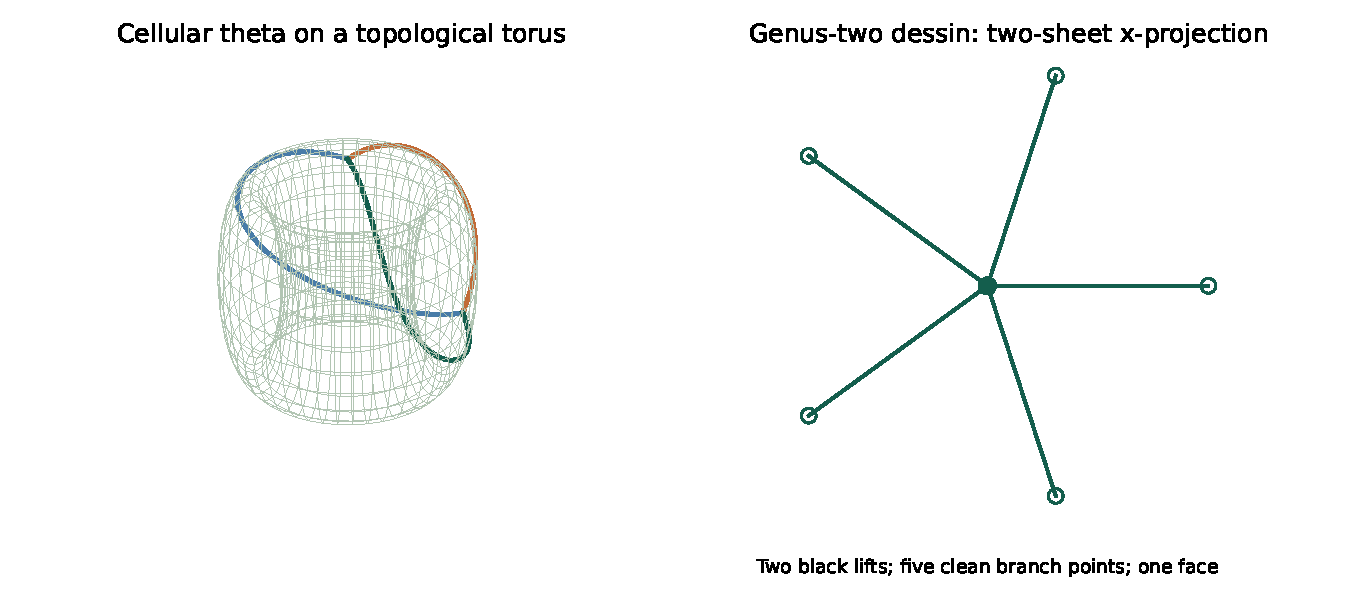
\includegraphics[width=\textwidth]{figures/dessin-carriers.pdf}
\caption{Two distinct kinds of faithful data display. Left: a topological torus embedding with the three periodic lifts of the theta graph. Right: the genus-two dessin's $x$-projection; every radial segment has two lifts. The right-hand disk is not the genus-two surface itself.}\end{figure}

\section{Larger genera and infinite hyperbolic windows}
The same exact family gives genus five ($m=11$, rank242), genus nine ($m=19$, rank722) and genus sixteen ($m=33$, rank2178). These ranks refer to the infinite completed orders over $k[[u]]$, not finite vector-space dimensions. The browser includes these examples and a four-dimensional rotation control: write $(x,y)\in\C^2$ in real coordinates $(x_1,x_2,y_1,y_2)$, rotate the $(x_1,y_1)$ plane, then project to three coordinates. The omitted coordinate and projected intersections are explicitly identified. This is a view of the affine double-cover sheets, not a claimed injective embedding of a compact higher-genus surface.

A separate example is the infinite regular hyperbolic $\{7,3\}$ tiling. Its heptagons have angles $2\pi/3$, so the defect formula gives area $5\pi-7(2\pi/3)=\pi/3$ at curvature $-1$. For a regular $\{p,q\}$ tiling, its central polygon's Poincar\'e circumradius is
\[
 r=\sqrt{\frac{\cos(\pi/p+\pi/q)}{\cos(\pi/p-\pi/q)}}.
\]
To derive this, bisect the polygon into right triangles with acute angles $\pi/p$ and $\pi/q$. The hyperbolic right-triangle identity is $\cosh R=\cot(\pi/p)\cot(\pi/q)$, while the disk radius is $r=\tanh(R/2)$. Substituting and applying elementary sum-to-product identities gives the formula. The condition $1/p+1/q<1/2$ ensures positive real radius.

A side is an arc of a circle with center $c$ and squared radius $|c|^2-1$, orthogonal to the unit disk. Its endpoints $a,b$ determine $\operatorname{Re}(a\bar c)=(|a|^2+1)/2$ and the analogous equation for $b$. Circle inversion gives its hyperbolic reflection
\[
 z\longmapsto c+\frac{|c|^2-1}{\bar z-\bar c}.
\]
If a side is a diameter, the circle formula is replaced by reflection in the line through the origin; the implementation handles that case separately. Reflecting adjacent polygons constructs finite windows of the infinite tiling. The implementation caps both depth and tile count and reports those bounds. It never calls a truncated window the whole infinite lattice. An optional Lorentz-hyperboloid view maps $z$ to $(2\operatorname{Re}z,2\operatorname{Im}z,1+|z|^2)/(1-|z|^2)$, satisfying $T^2-X^2-Y^2=1$. Its metric is Lorentzian ambient data, not the Euclidean metric of the rendered mesh. A finite compact surface quotient, its side pairings and an arithmetic correspondence would require separate certificates. The current lattice patch supplies none of them.

\section{What a three-dimensional view can claim}
The genus-one examples use a standard torus parameterization
\[
 ((R+r\cos v)\cos u,(R+r\cos v)\sin u,r\sin v),\quad R>r>0.
\]
The theta paths lift from $(0,0)$ to $(1/3,1/3)$ with translation vectors $(0,0),(-1,0),(0,-1)$ in the universal covering plane. Their interiors are disjoint on the quotient, and their complement is a disk; the induced rotations at the two black vertices give the one-face theta dessin. The elliptic square uses the two fundamental loops. These are topological realizations; the induced Euclidean torus metric is not asserted to be the constant-curvature or uniformizing metric of the algebraic curve.

For $m\ge5$, the companion instead plots a three-real-coordinate projection of the two sheets of $y^2=x^m-1$. Branch cuts, changes of sheet and the compact point at infinity remain part of the mathematical construction. Projected sheets can meet. No injective embedding or numerical uniformization follows from a screen image. The Sage source gives exact passports, quivers, forbidden pairs and determinant calculations. The installed \texttt{sage} launcher on this machine points to a missing application, so those Sage scripts are supplied but have not been executed in Sage in this milestone. Exact stdlib Python checks independently verify the displayed permutations, genus and ramification counts.

\section{Finite clocks and cross-backend agreement}
For $d\ge2$, let $Ue_j=\zeta^j e_j$, $Ve_j=e_{j+1}$, with $\zeta=e^{2\pi i/d}$. Then
\[
 UV=\zeta VU,\quad U^d=V^d=I.
\]
Applying the two sides to $e_j$ proves the first identity, including the wraparound because $\zeta^d=1$. The discrete Fourier matrix prepares the uniform superposition. The executable comparison applies $F$, then $U$, then $V$, on a four-level carrier; its relative phases are nonconstant. Cirq, Qiskit and PennyLane statevectors are compared to the reference vector. Strawberry Fields realizes the same $U(4)$ matrices on the single-photon subspace of four optical modes and compares the entire density block, including its off-diagonal phases. Preparing a Fock state need not leave the simulator's internal representation marked pure, so reading only a ket would be incorrect.

The photonic cutoff two is exact for this passive, single-photon computation: photon number is preserved and no mode ever contains more than one photon. This justification does not extend to arbitrary squeezing or multiphoton simulations. Separate NVIDIA cuQuantum and CUDA-Q adapters and pinned upstream forks are provided. GPU execution is not performed on this Mac; source availability is distinct from a successful accelerator run.

\chapter{Quantum feature models and auxiliary compression}
\label{book:learning}
These preserved experiments have distinct objectives. Local Ising regressors approximate selected coarse couplings but omit normalization and a full iterated action. QCNN compression, photonic principal-axis alignment and the Harper surrogate are auxiliary benchmarks. Actual partition-preserving RG and a trained full-action approximation are developed in Chapter~\ref{rg:chapter}. Here the exact targets, held-out samples, recorded seeds, classical optimizer and feature readouts are retained without calling these different objectives a complete RG flow.

\section{Exact teacher data from Ising decimation}
For spins $s_1,s_2,s_3\in\{-1,1\}$, summing the middle spin gives
\[
 \sum_{s_2}e^{K_1s_1s_2+K_2s_2s_3}
 =2\cosh(K_1s_1+K_2s_3)
 =A e^{K' s_1s_3},
\]
where
\[
 K'=\tfrac12\log\frac{\cosh(K_1+K_2)}{\cosh(K_1-K_2)}
 =\operatorname{arctanh}(\tanh K_1\tanh K_2),\quad
 A=2\sqrt{\cosh(K_1+K_2)\cosh(K_1-K_2)}.
\]
Checking $s_1s_3=\pm1$ proves the identities. Thus the normalization and coupling have separate roles. The network below learns $K'$, not the full partition-function normalization $A$.

For a three-valent star, let $s=(s_1,s_2,s_3)$ be boundary spins and sum its center. The exact boundary logarithmic weight is
\[
 f_K(s)=\log\bigl(2\cosh(K_1s_1+K_2s_2+K_3s_3)\bigr).
\]
Fourier expansion on the Boolean cube is orthogonal for $2^{-3}\sum_s$. The symmetry $f_K(-s)=f_K(s)$ removes every odd monomial. Consequently
\[
 f_K(s)=c(K)+\sum_{i<j}J_{ij}(K)s_is_j,\quad
 J_{ij}=2^{-3}\sum_s f_K(s)s_is_j.
\]
This proves the zero-field star-to-triangle reduction and supplies exact labels. Such trivalent patches occur at the black vertices of the theta dessin. The associated Ising Hamiltonian is a finite model on that graph, not a faithful representation of its completed surface order.

\section{Shared quantum graph convolution}
The input patch $(K_1,K_2)$ is encoded by
$R_y(K_1)\otimes R_y(K_2)|00\rangle$. Two layers of local $R_y,R_z$ rotations, a CZ entangler after each layer, and a final CNOT define an eight-parameter circuit $Q_\theta$. The three features are
\[
 z_\theta(K)=\bigl(\langle Z_0\rangle,\langle Z_1\rangle,\langle Z_0Z_1\rangle\bigr).
\]
A shared affine head predicts $\widehat K'=w\cdot z_\theta+b$. Twelve trainable parameters include the four readout coefficients. Independent samples are drawn uniformly from $[0.05,1.7]^2$: ninety are used for training and thirty are held out. The loss is the mean-square error against exact decimation. The independent constant predictor is fitted only on training targets.

For a gate $e^{-itP/2}$, $P^2=I$, and a fixed state and observable, the expectation has the form $a+b\cos t+c\sin t$. Hence
\[
 \partial_t z=\tfrac12\bigl(z(t+\pi/2)-z(t-\pi/2)\bigr).
\]
Each gate parameter occurs once. The code differentiates the expectation features with this formula and then applies the classical chain rule to the squared loss and affine head. Applying parameter shift to the squared loss itself would generally give a wrong gradient. A central finite-difference check of the implemented full loss gradient is recorded.

\section{QCNN compression with a genuine pooling channel}
The four-site periodic transverse-field Ising Hamiltonian is
\[
 H(h)=-\sum_{(i,j)\in C_4}Z_iZ_j-h\sum_{i=0}^3X_i.
\]
We diagonalize its $16\times16$ Hermitian matrix at thirty-six fields in $[0.15,2.4]$, using the normalized lowest eigenvectors as input states. Every fourth field, starting at index zero, is held out. The circuit has two shared-layout local rotation layers with CZ edges on $C_4$, followed by CNOTs $(0,2)$ and $(1,3)$. Its sixteen parameters are optimized to minimize
\[
 \mathcal L(\theta)=1-\frac1{N_{\rm train}}\sum_j
 \langle\psi_j|Q_\theta^*(I_{01}\otimes|00\rangle\langle00|_{23})Q_\theta|\psi_j\rangle.
\]
The output on retained qubits is
\[
 \mathcal E_\theta(\rho)=\operatorname{Tr}_{23}(Q_\theta\rho Q_\theta^*).
\]
Its Kraus maps are $K_b=(I\otimes\langle b|)Q_\theta$, so
$\sum_bK_b^*K_b=I$. Thus it is completely positive and trace preserving. For $\rho\ge0$ and any $v$, each summand $v^*K_b\rho K_b^*v$ is nonnegative; cyclicity of the finite trace proves trace preservation. The Lean interface verifies the finite-matrix positivity and trace statements with explicit completeness hypotheses. It does not formalize the optimizer or claim convergence of an infinite renormalization flow.

The compression loss is the weight discarded by the chosen vacuum projection. Its successful decrease measures improved concentration for this finite input family. It does not imply exact recovery of arbitrary four-qubit states, an isometry from dimension sixteen to four, or a critical fixed-point construction. The held-out loss remains appreciable, and is reported without calling the model lossless.

\section{A larger genus-four nine-qubit example}
The $m=9$ hyperelliptic dessin has genus four and completed-order rank162. Its nine edge labels index a permitted quiver cycle. A separate finite transverse-field Ising model is placed on this nine-cycle, with Hilbert-space dimension512. This uses the dessin's combinatorics, without claiming a faithful representation of its infinite order.

The larger experiment uses twelve ground states over fields $h\in[0.2,1.9]$, with nine training and three held-out states. These are numerical lowest-eigenstate approximations. The residual alone is not a rigorous lowest-energy certificate. A sparse Hermitian eigensolver has maximum recorded eigenpair residual $1.32\times10^{-13}$. The circuit has two layers of local $R_y,R_z$ gates and nearest-neighbor CZ around the cycle, with thirty-six parameters. Four CNOTs connect retained to discarded qubits, and tracing out four leaves a five-qubit output. Actual PennyLane gate simulation and parameter-shift gradients train for fifty updates. Final training and held-out discard losses are approximately $0.548$ and $0.409$. These substantial residuals are reported: this architecture is not an accurate lossless coarse graining. It is a reproducible larger testbed, with saved parameters, held-out examples and numerical ground-state residuals. The local page permits comparison with the smaller four-qubit model, while retaining their different data families and capacities.

\section{Quantum-feature graph attention}
Three two-qubit patch encoders use the same eight circuit parameters on the three pairs of the Ising star. Let their features be $z_e\in\R^3$. A learned query $q$ defines
\[
 \alpha_e=\frac{e^{q\cdot z_e}}{\sum_f e^{q\cdot z_f}},\quad
 c=\sum_e\alpha_e z_e,\qquad
 \widehat J_e=w_{\rm local}\cdot z_e+w_{\rm context}\cdot c+b.
\]
There are eighteen trainable parameters. One hundred star couplings are sampled from $[0.1,1.5]^3$, with seventy-five training and twenty-five held-out examples. The objective compares the three predictions with the exact Boolean-Fourier couplings above. The nonlinear attention head is differentiated by central differences of the complete training objective. This experiment is quantum-feature attention with a classical softmax head; it is not a fully coherent attention algorithm. The scalar labels do not assert permutation equivariance under conventions the implementation has not checked.

\begin{center}
\begin{tikzpicture}[node distance=5mm, every node/.style={font=\small}, b/.style={draw,rounded corners,align=center,text width=32mm,minimum height=13mm}]
\node[b] (a) {Exact finite\\physics data};
\node[b,right=of a] (b) {Shared quantum\\patch circuits};
\node[b,right=of b] (c) {Classical head\\or attention};
\node[b,right=of c] (d) {Held-out loss\\and exact checks};
\draw[-{Latex}] (a)--(b);\draw[-{Latex}] (b)--(c);\draw[-{Latex}] (c)--(d);
\end{tikzpicture}
\end{center}

\section{Photonic Gaussian pooling}
The Strawberry Fields experiment prepares two modes with opposite real squeezing $r$ and $-r$, then applies a fixed unknown-to-the-optimizer beam splitter angle $\alpha=0.47$. A learned shared beam splitter $\theta$ is optimized on twelve of sixteen squeezing values in $[0.1,0.9]$, holding out every fourth value. With $\hbar=2$, the covariance convention is $(x_0,x_1,p_0,p_1)$. The objective is
\[
 \operatorname{Var}(x_0)+\operatorname{Var}(p_1)
 =2\left[e^{-2r}\cos^2(\alpha+\theta)+e^{2r}\sin^2(\alpha+\theta)\right].
\]
This follows by applying the real beam-splitter rotation to the diagonal covariance of the two squeezed modes. Since $r>0$, its minimum occurs at $\theta=-\alpha$ modulo $\pi$, with value $2e^{-2r}$. The code trains the angle with central-difference gradients and compares its result with this known optimum. Pooling subsequently discards a mode; the experiment itself optimizes principal axes before that discard. It is a Gaussian finite-mode surrogate, not a demonstration of an interacting field-theory RG flow.

\begin{figure}[ht]\centering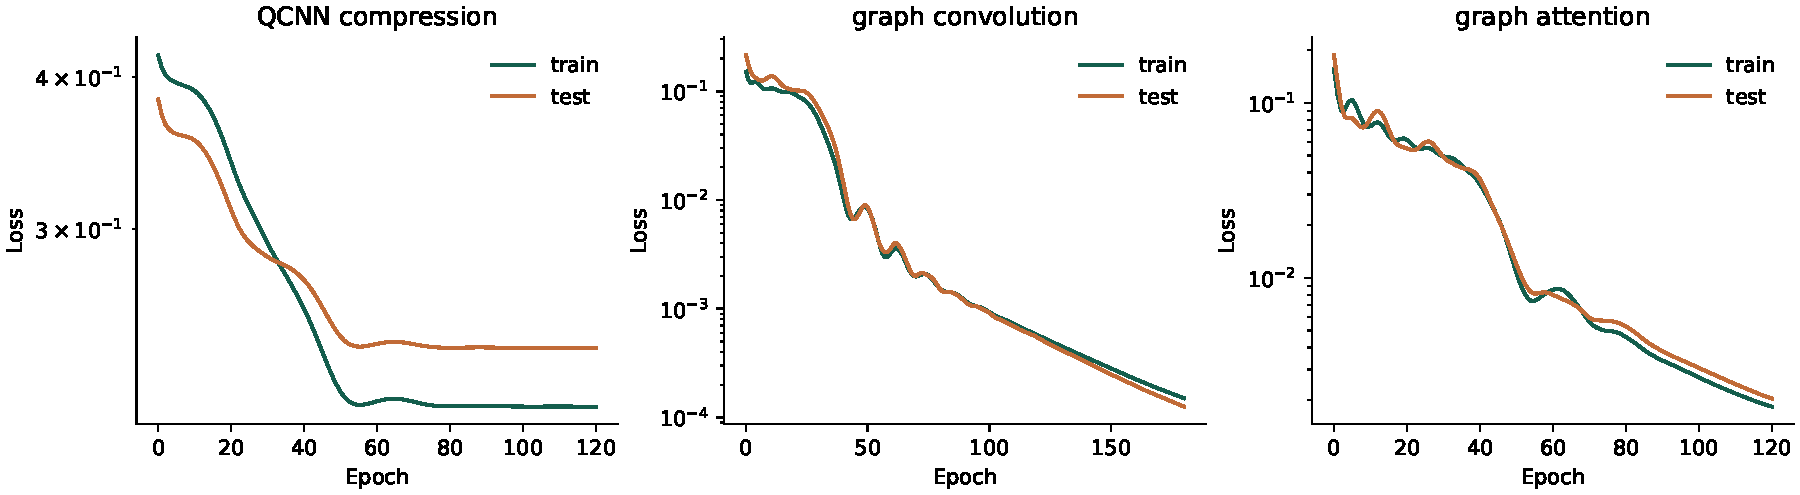
\includegraphics[width=\textwidth]{figures/training-curves.pdf}
\caption{Actual PennyLane CPU training runs, seed 20261103. Green is training loss; orange is held-out loss. Architectures have different objectives, so their vertical scales are not cross-model performance rankings.}\end{figure}
\begin{figure}[ht]\centering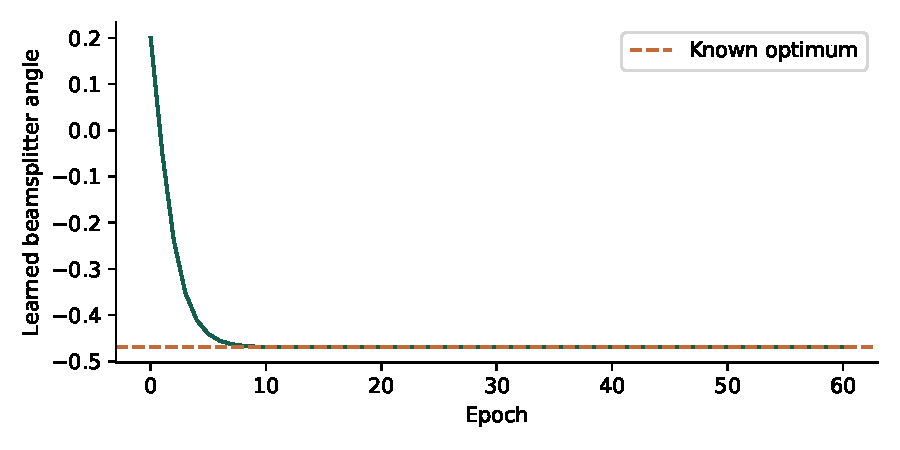
\includegraphics[width=.7\textwidth]{figures/photonic-angle.pdf}
\caption{Actual Strawberry Fields Gaussian simulation: the learned principal-axis angle approaches its independently known optimum.}\end{figure}
\begin{center}\small
\begin{tabular}{lrr}\toprule
Model & Initial held-out loss & Final held-out loss\\\midrule
Four-qubit QCNN compression & 0.38332 & 0.239725\\
Shared quantum graph convolution & 0.213652 & 0.000125897\\
Quantum-feature graph attention & 0.187065 & 0.00204477\\
\bottomrule\end{tabular}\end{center}


\section{Reproduction and limits of the evidence}
The scripts in \texttt{examples/quantum} specify each circuit, data generator, random seed and optimizer. The approved isolated environment is recorded in \texttt{requirements-cpu.lock}; existing environments and all pinned Lean toolchains remain unchanged. NumPy reference and actual PennyLane runs are saved separately. Cross-framework tests exercise a nontrivial Fourier/clock/shift state, not just a vacuum on which every diagonal clock is invisible. The Strawberry Fields run uses its Gaussian backend for training and its Fock backend for the separate one-photon comparison.

The companion's checkpoint slider selects a saved loss checkpoint. Its held-out examples use final weights; no intermediate predictions are implied. There are no hardware shots, cloud jobs or accelerator benchmarks. The training/test splits are deterministic interpolation tests on small synthetic families, not out-of-distribution or broad physical-validity tests. A model can help rank a proposed construction; it cannot discharge arithmetic holomorphy, determinant convergence, positivity or zero-location obligations merely by achieving low loss.

\chapter{Reading an architecture from its tensors}
\label{book:architecture}
The trained models of Chapter~\ref{book:computations} and the ToricGT
references have a common computational interface: a finite directed acyclic
graph whose vertices contain actual tensors and whose edges record the
inputs to each operation. The local inspector at
\url{http://127.0.0.1:8765/architecture.html} makes this graph navigable.
Its scene is a computation graph, not a hardware layout or a physical
embedding of the infinite surface order. The source code and numerical
records are part of the project.

\section{Three distinct kinds of evidence}
The twenty-two saved cases cover six trained CPU model families and six
fixed-weight reference variants. The QCNN4 and QCNN9 weights, shared
two-qubit convolution, quantum-feature attention, Gaussian photonic pooling
and finite Harper hybrid are replayed without further optimizer steps.
The classical TokenGT-style, tropical, block-ring, attention-hybrid and two
expert-routing variants use explicit seeded weights. They are executable
miniatures, not upstream trained language-model checkpoints. The adjustable
forward clock is a separately computed finite carrier. GPU and hardware
execution remain unavailable, and optional upstream heads remain proposals
unless their own numerical evidence is supplied.

The record contains the source/checkpoint hashes, seed, conventions,
formulas, shapes, axes, parameter values and checked errors. Each saved
record is immutable and content addressed; its SHA-256 is verified before
the interface accepts it. The inspector never changes the trained weights.
Selecting a forward-operation step is not selecting a training epoch.

\section{Shapes explain the operation}
Two different attention mechanisms illustrate why the axes matter.
The trained quantum-feature model produces three feature vectors,
\[
 F\in\R^{3\times3},\quad \ell=Fq\in\R^3,\quad
 \alpha=\operatorname{softmax}(\ell),\quad c=\alpha^{\mathsf{T}}F\in\R^3.
\]
Softmax here runs over three patches. The classical reference has seven
token positions, including one padded node, model width six and two heads.
After projection and splitting, its $Q,K,V$ have shape
$[1,2,7,3]$. These heads are different from the three observables of the
quantum circuit. Its $Q,K$ also undergo the source's maximum shift and
Euclidean normalization before dot scores.

\begin{center}
\begin{tikzpicture}[>=Stealth,every node/.style={font=\small},
 box/.style={draw,rounded corners,align=center,text width=4.5cm,minimum height=.8cm}]
\node[box] (q) at (0,0) {Trained quantum patches\\$F:[3,3]$};
\node[box] (a) at (0,-1.4) {Patch softmax\\$\alpha:[3]$, $c:[3]$};
\node[box] (h) at (0,-2.8) {Local/context affine heads\\prediction $[3]$};
\node[box] (t) at (6,0) {Fixed graph tokens\\$X:[1,7,6]$};
\node[box] (s) at (6,-1.4) {Projected/normalized heads\\$Q,K,V:[1,2,7,3]$};
\node[box] (v) at (6,-2.8) {Softmax or max-plus context\\$[1,2,7,3]$};
\draw[->] (q)--(a);\draw[->] (a)--(h);
\draw[->] (t)--(s);\draw[->] (s)--(v);
\end{tikzpicture}
\end{center}
The shape labels are literal exported dimensions. The two columns are
different finite models; no equivalence of their learned functions is
asserted.

For tropical aggregation, a scalar output is
\[
 C_{bhic}=\max_{j\text{ legal}}
       \bigl(S_{bhij}+V_{bhjc}\bigr),\qquad
 S=QK^{\mathsf{T}}/\sqrt{d_{\rm head}}.
\]
The inspector shows every maximizing key and the gap between the largest
two legal values. A tie means equality of computed floating-point values,
not a symbolic equality certificate. A query with no legal key has zero
context by an explicit guard. Invalid block entries are stored as zero
\emph{with a validity mask}; including these zeros in a maximum would be
incorrect. Softmax weights displayed in tropical records are comparison
diagnostics rather than the tropical aggregation rule.

Soft-MoE dispatch normalizes across valid tokens for each expert-slot;
combination normalizes across expert-slots for each valid token. These are
different axes. Strict-prefix slots exclude the current and later token
indices, while equal-rank attention can permit different tokens with the
same reveal rank. The two rules must not be conflated into a stronger
causality assertion. Likewise padding can acquire projection bias in a
residual, so its mask must remain in later routing and pooling.

\section{Quantum and Gaussian inspection}
The stored StatePrep input precedes the displayed circuit. The variational
gates have their exact wire order and angle metadata. Qubit zero is most
significant. For QCNN9, the final CNOT targets start at wire five; the
retained density matrix has shape $[32,32]$, not a five-qubit pure state
obtained by discarding amplitudes. The partial trace follows the unitary
gates and is distinct from their dimension-preserving action.

The photonic model uses covariance order $(x_0,x_1,p_0,p_1)$ and
$\hbar=2$. Its ellipse is a one-standard-deviation contour of a selected
two-coordinate Gaussian marginal, with the marginal covariance taken from
the actual intermediate record. It is not a plot of a trained interacting
field theory. The Harper page separately displays the learned proposal and
the fifteen exact rational principal-minor certificates. Rejected proposals
are labelled as repaired. The carrier uses backward $V$, so $VU=iUV$;
the live forward-clock example instead has $UV=\omega VU$.

\section{Spatial calculations and guided navigation}
The interaction reference is Brendan Bycroft's \emph{LLM Visualization},
reviewed at the pinned source revision recorded in
\path{planning/reference-inspector/source-manifest.json}.
Its model overview and self-attention walkthrough place the narrative
beside dimensioned tensor planes, parallel query/key/value projections,
attention heads and residual paths. The source's picking code maps a
selected output cell to input rows or columns and dot-product terms;
its camera code interpolates toward walkthrough targets. These specific
mechanisms motivate the local redesign. Reference hover inspection was
limited by a renderer crash; source inspection is distinguished from
successful live observation.

The local implementation uses original browser code and the project's
own immutable records. Its spatial scene follows dependency ranks and
semantic lanes, rather than putting every operation in an identical card.
A tensor's dimensions determine its grid; head planes, selected literal
coordinates and level-of-detail windows remain labelled. Overview retains
the whole recorded computation, while a focused step moves toward its
neighbourhood. The narrative gives the actual operation and evidence type.
Supported cell expansions show numerical input terms and their computed
result; other operations retain graph dependencies without inventing a
scalar derivation. Surface and circuit views explain a separate geometric
or physical interpretation of the finite carrier.

The rendering is a lightweight axonometric projection rather than a copy
of the reference's WebGL engine. Neither perspective effects nor a
quantum-state array make an attention model a coherent quantum transformer.
Checkpoint replay, fixed-weight reference calculations and separately
proposed extensions keep their different status throughout the interface.

\section{A reproducible way to explore}
Choose an evidence category and example, then a step. Clicking an input
follows its recorded dependency. Head/token/coordinate controls select
literal array slices; paging exposes large states without pretending that a
small viewport is the entire tensor. Color is a display convention and the
selected coordinate gives its numerical real and imaginary parts. A zero
amplitude has undefined phase and is labelled accordingly. Playback visits
the forward pass, and stops when cases change or the tab becomes hidden.
Orbit and zoom change the view, not the state or physical model.

The shared numerical records have independent quantum-backend and scalar
reference checks. Browser checks exercise all saved cases, coordinate
selection, masks, playback, view controls, circuits, covariance and certificate
panels. These computational checks do not imply complete Lean formalization,
generalization beyond the samples, quantum advantage or the arithmetic
positive-determinant comparison. The general path/category and arithmetic
interfaces remain the research obligations described in the final chapters.

% Generated shared reviewed material.
\section{ConvexTok: certified path vocabularies}
\label{convextok:section}
The words ``token'' and ``graph'' have two different roles here. A TokenGT
position represents a node or edge with features and incidence metadata.
A tokenisation position instead represents a boundary in a word; an edge
jumps across a contiguous substring. ConvexTok, introduced by Tempus,
Whittington, Schmidt, Komm and Pimentel,
\emph{Tokenisation via Convex Relaxations},
\href{https://arxiv.org/html/2605.22821v1}{arXiv:2605.22821v1},
optimises the second representation. We derive its small finite
formulation, reproduce its six-word example, and give new certified
examples for finite arrow-word corpora of our infinite surface algebras.
This supplies an auditable compression layer; it does not identify the two
kinds of token or change a trained graph model.

\subsection{A vocabulary controls many occurrences}
Let $\mathcal D=(w_1,\ldots,w_N)$ be a finite multiset of nonempty words over
a mandatory alphabet $\Sigma$. For each word introduce boundary vertices
$0,\ldots,|w_n|$. Include an edge $(i,j)$ for each allowed contiguous token
$w_n[i:j]$. All single-symbol edges are free in the vocabulary budget,
but cost one each in the segmentation objective. Longer candidates form
a finite set $C$. Equal strings have the same colour even when they occur
in different words or positions. Candidates never cross word boundaries.

Write $x_e$ for occurrence flow and $c_t$ for selection of token type $t$.
Use incidence entries $-1$ at an edge's source and $+1$ at its target.
For each word let $d$ be $-1$ at its initial boundary and $+1$ at its final
boundary. Separate unit-flow equations are equivalent to joining adjacent
word terminals as in the paper: each word boundary must carry one unit,
and there are no edges across words. The finite programme is
\begin{equation}\label{convextok:lp}
 \begin{aligned}
 L_K=\min\quad &\sum_e x_e\\
 \text{subject to}\quad &Bx=d,\qquad 0\le x_e,c_t\le1,\\
 &x_e\le c_t\quad(e\text{ an occurrence of }t\in C),\qquad
 \sum_{t\in C}c_t\le K.
 \end{aligned}
\end{equation}
Requiring $x_e,c_t\in\{0,1\}$ gives the integer problem. On the acyclic
position graph its flow is one path per word, hence one segmentation.
Conversely any segmentation with at most $K$ extra token types gives such
an integer point. Consequently the LP optimum is a lower bound for the
integer optimum $I_K$. The constraint is per occurrence: selecting
$\mathtt{ab}$ once permits both occurrences in $\mathtt{abab}$, whose
cost is two. Replacing these constraints by
$\sum_{e:\,t(e)=t}x_e\le c_t$ would incorrectly prohibit that reuse.

For a fixed discrete vocabulary $V\supseteq\Sigma$, the exact segmenter is
the backward recurrence
\[
 D(n)=0,\qquad
 D(i)=1+\min_{t\in V:\,w[i:i+|t|]=t}D(i+|t|).
\]
It returns a shortest path and a decoding by concatenation. Longest-first
greedy need not do so: for $w=\mathtt{abcd}$ and extra vocabulary
$\{\mathtt{ab},\mathtt{bcd}\}$ it returns
$\mathtt{ab}|\mathtt c|\mathtt d$, whereas the optimum is
$\mathtt a|\mathtt{bcd}$. This segmentation issue is separate from BPE's
greedy construction of the vocabulary itself.

\subsection{An exact lower bound needs a feasible certificate}
A floating solver's proposed objective alone is insufficient for an
exact lower-bound claim. Our original CPU checker writes the LP in the
form
\[
 \min q^{\mathsf T}v,\qquad Av=b,\quad Gv\le h,\quad v\ge0,
\]
where $v=(x,c)$ and $G$ includes every upper-bound row $v_i\le1$.
It uses SciPy/HiGHS from the already approved environment to propose
primal and dual solutions, reconstructs rational entries, and then checks
\emph{every} condition with exact rational arithmetic:
\[
 Av=b,\quad Gv\le h,\quad v\ge0,\qquad
 z\le0,\quad A^{\mathsf T}y+G^{\mathsf T}z\le q,
 \qquad q^{\mathsf T}v=b^{\mathsf T}y+h^{\mathsf T}z.
\]
These are executable rational witnesses, not a claim that floating-point
optimisation itself is a proof assistant.
\begin{proposition}[Finite rational certificate]
Every feasible primal $v'$ obeys
$q^{\mathsf T}v'\ge b^{\mathsf T}y+h^{\mathsf T}z$ for any dual pair
satisfying the displayed inequalities. Equality with one feasible $v$
certifies the exact LP optimum.
\end{proposition}
\begin{proof}
Since $v'\ge0$, the componentwise dual inequality gives
\[
 q^{\mathsf T}v'\ge y^{\mathsf T}Av'+z^{\mathsf T}Gv'
 \ge y^{\mathsf T}b+z^{\mathsf T}h.
\]
The second inequality uses $z\le0$ and $Gv'\le h$. Equality therefore
matches a lower and an upper bound.
\end{proof}
Independently, our checker exhausts every size-$K$ subset of $C$ and runs
the shortest-path segmenter on each. This covers the at-most-$K$ problem,
because adding candidate tokens cannot increase a shortest-path cost.
For $K>|C|$, all candidates suffice. Every stored witness is checked;
deliberately perturbed primal and dual witnesses are rejected.

\subsection{Three rounding rules and worked numerical gaps}
The paper's Det rule chooses the $K$ largest $c_t$; Bias chooses the
$K$ largest $c_t/|t|$; Int retains only values essentially equal to one.
Our certificates are rational, so Int uses exact equality to one and
Det/Bias use lexicographic tie-breaking. After choosing tokens we
recompute a discrete shortest path; a fractional flow is not itself a
tokenisation. An integral colour in one LP solution need not be present
in every optimum. For example, with word $\mathtt{abc}$ and candidates
$\mathtt{ab},\mathtt{bc}$, either single-token choice is optimal.

The paper's example is
\[
 \mathcal D_0=(\mathtt{abc},\mathtt{abd},\mathtt{abe},
              \mathtt{bc},\mathtt{bd},\mathtt{be}),\qquad K=3.
\]
The mandatory-symbol count is fifteen. BPE first creates $\mathtt{ab}$,
saving three positions, then two merges save only one each: its cost is
ten. Choosing $\mathtt{bc},\mathtt{bd},\mathtt{be}$ instead gives nine.
Our exact primal/dual pair has value nine, and all $\binom73=35$
candidate vocabularies confirm $L_3=I_3=9$. All three rounding rules give
nine on the saved LP solution.

Our first new example is
\[
 \mathcal D_1=(\mathtt{cbcbc},\mathtt{cbca},
              \mathtt{cbabac},\mathtt{caaab}),\qquad K=2.
\]
One optimal fractional vocabulary has
\[
 c_{\mathtt{cbc}}=\tfrac12,\qquad
 c_{\mathtt{caaab}}=\tfrac12,\qquad
 c_{\mathtt{cbabac}}=1,
\]
with all other values zero. Its per-word costs are $3,3,1,3$, totalling
ten; the rational dual certifies optimality. The integer optimum is
eleven, witnessed by vocabulary
$\{\mathtt{caaab},\mathtt{cbabac}\}$ with costs $5,4,1,1$ and confirmed
by all $\binom{30}{2}=435$ vocabularies. Det and Bias also yield eleven,
while Int yields fifteen. The LP is therefore genuinely fractional even
though its objective is an integer.

A second original corpus,
\[
 (\mathtt{aaaab},\mathtt{baaccb},\mathtt{aac},
   \mathtt{babaab},\mathtt{cbbbca}),\qquad K=2,
\]
has $L_2=31/2<I_2=16$. Its nonzero colour weights are
$c_{\mathtt{aa}}=c_{\mathtt{babaab}}=1/2$ and
$c_{\mathtt{cbbbca}}=1$. The per-word fractional costs are
$7/2,11/2,5/2,3,1$. Exhausting $\binom{42}{2}=861$ vocabularies certifies
the integer value. These examples demonstrate a relaxation gap; they do
not supply a universal approximation ratio for rounding.

\subsection{Application to permitted paths on actual higher-genus dessins}
Set $m=2g+1$ for $g=2,4$, and retain the existing clean dessin of
$y^2=x^m-1$, $\beta=x^m$. On $H=\{0,\ldots,2m-1\}$ put
\[
 \sigma=(0\ \cdots\ m-1)(m\ \cdots\ 2m-1),\qquad
 \alpha(h)=h+m\pmod{2m},\qquad \tau=\sigma^{-1},\quad\phi=\alpha\tau.
\]
There are two vertex cycles, $m$ edges and one face, so
$2-2g=2-m+1$. Its polynomial algebra is the infinite locally gentle
algebra
\[
 A_g=kQ/(a_h a_{\phi h}:h\in H),\qquad
 a_h:[h]\longrightarrow[\tau h].
\]
Here products are written in travel order: $ab$ traverses $a$ first and
then $b$. A left-operator matrix convention reverses these products.
Define the nonzero permitted word
$P(h,r)=a_h a_{\tau h}\cdots a_{\tau^{r-1}h}$. Our finite multiset is
\[
 \big(P(0,m+2),P(0,m+2),P(m-1,4),
      P(m,m+2),P(2m-1,4)\big).
\]
Each arrow label is one alphabet symbol, even when its printed label has
several characters. The duplicate first word retains its multiplicity.
We allow every occurring subpath of length two or three as an extra
candidate. The LP bound consequently concerns this explicitly restricted
candidate set, not arbitrary-length vocabularies.
\begin{center}\small
\begin{tabular}{rrrrrr}
\toprule
$g$ & $m$ & $|C|$ & symbol count & $L_2=I_2$ & subsets checked\\
\midrule
2&5&20&29&19&190\\
4&9&36&41&31&630\\
\bottomrule
\end{tabular}
\end{center}
The exact witnesses attain these values, and Det/Bias/Int all attain
them on the saved LP solutions. A token names a finite permitted subpath;
concatenation recovers every original arrow, hence its quiver endpoints
and original path length. This is finite corpus compression, not a
finite-dimensional quotient of $A_g$. Arbitrary token concatenations may
fail composability and need their own endpoint checks. Neither an algebra
homomorphism on a freely generated token algebra nor a representation of
arbitrary completed formal sums is asserted. The completed order still
has rank $2m^2$ over $k[[u]]$; its rank, coefficients, multiplication,
relations and modules are not reduced by counting tokens.

The companion laboratory at
\url{http://127.0.0.1:8765/convextok.html} exposes the position DAG,
literal fractional flows, vocabularies and discrete segmentations.
Its five corpora and sixteen budget cases have sixteen exact
primal/dual certificates and 2,312 exhausted integer vocabularies in
total. The browser independently recomputes segmentation costs from
local arrays; it does not solve a new LP when a user changes a vocabulary.
The primary paper's NLP training and large GPU experiments are not
reproduced. Compression of a finite path corpus proves no module or
Fukaya equivalence, arithmetic determinant comparison, or GRH statement.


\chapter{Quantum TokenGT, concept navigation and error correction}
\label{qtoken:chapter}
This chapter connects executed finite methods through the same physical RG
teacher. The completed order, ribbon dessin, physical Hamiltonian, token
sequence and auxiliary quantum circuit retain their different dimensions.
The surface is not reconstructed from a neural embedding, and the network
is not silently declared a module over its completed order.

\section{Node and edge tokens with a quantum feature map}
The genus-two clean dessin of Chapter~\ref{rg:chapter} has five quiver
vertices and DVR-rank 50. Its physical $ K_{2,5}$ incidence model has seven
spin nodes and ten incidence edges. Our TokenGT-style input has these 17
valid node/edge tokens and one masked padding position. Each token carries
its type and endpoint metadata through an explicit three-angle encoding.
The normalized auxiliary state uses $ R_y $ data gates, fixed $ R_z $ rotations,
CNOT $_{01}$, CNOT $_{12}$ and fixed $ R_x $ rotations. The measured features are
\[
 (\langle Z_0\rangle,\langle Z_1\rangle,\langle Z_2\rangle,
   \langle Z_0 Z_1\rangle,\langle Z_1 Z_2\rangle,\langle Z_0 Z_2\rangle).
\]
These are three feature qubits per token, not the seven physical spin sites
or a faithful representation of the infinite order. The quantum feature map
is frozen; the Q/K/V matrices and nonlinear readout are trained. A separate
literal replay of the pinned elliptic-theta fixture is retained with its
own input hash and category boundary. The physical RG training input is the
genus-two incidence graph, not that different theta fixture.

With $ Q=XW_Q $, $ K=XW_K $, $ V=XW_V $ and $ S=QK^{\mathsf{T}}/\sqrt{6}$, define,
on valid query/key indices,
\[
 C^{\rm soft}=\operatorname{softmax}(S)V,
 \qquad C^{\rm trop}_{ir}=\max_j(S_{ij}+V_{jr}),
 \qquad C^{\rm hybrid}=\tfrac 12(C^{\rm soft}+C^{\rm trop}).
\]
Padding is masked in both softmax and max-plus operations and in pooling.
The tropical output is a componentwise max-plus aggregation, with actual
maximizing-key witnesses. It is not merely an argmax-key copy. A tanh
context/residual pool and classical head predict all 32 coarse logweights,
including the constant. These are quantum--classical transformers on measured
features, not a coherent softmax unitary. TokenGT \cite{QTokenGT} motivates
the node/edge organization; no general upstream expressivity or benchmark
theorem is asserted for this compressed feature map. Numerical token-row
permutation transport is checked, separately from arbitrary graph-relabel
invariance and information lost by the encoding.

\section{Matched training on an actual effective action}
Four models use the same 120/40 split,40 OOD cases, seed 20261103, shared
initialization/batches,900 Adam updates and 1,076 trained parameters each.
The fourth uses six classical trigonometric features and the same hybrid
head. The teacher is exactly $\mathcal RV $ from the seven-spin physical
model, so partition, constant and retained-observable errors have physical
meanings. The controlled input has three tied parameters, not 31 freely
varied output couplings.
\begin{center}\small
\begin{tabular}{lrrrr}
Features/context&action RMSE&log $ Z $ RMSE&magnetization RMSE&mean TV\\\hline
Quantum/softmax&.10261&.09247&.01773&.03420\\
Quantum/tropical&.06530&.05923&.01846&.02167\\
Quantum/hybrid&.10125&.09653&.02709&.03212\\
Classical/hybrid&.04878&.04712&.01565&.01663
\end{tabular}
\end{center}
The classical baseline has lower held-out full-action error. Quantum OOD
RMSE ranges from.555 to.763, versus.591 for the classical hybrid. One seeded
experiment establishes neither quantum advantage nor general OOD robustness.
The raw cases, every optimizer step and saved parameters are preserved.
The tensor inspector replays actual token states, gates, Q/K/V, masks, scores,
contexts and readout, and separately exposes the trained concept critic and
continuous-GFlowNet MLP/density computations, with synchronized physical and algebraic support labels.

\section{A defined mutual-information objective for concept directions}
Let $ z\in\R^6$ be a pooled embedding. We learn three normalized directions
$ B_1,B_2,B_3$ and a critic; their span need not be the whole embedding space.
Choose $ C $ uniformly among the six direction/sign codes and define
\[
 \Delta=\tanh(0.3 z+0.7\operatorname{sign}(C)B_{\operatorname{dir}(C)})
             -\tanh(0.3 z).
\]
A fixed vector is not a random variable: the random objects here are the
intervention code and its induced embedding change. The GraphCG-inspired
\cite{QGraphCG} objective is cross entropy for predicting $ C $ from $\Delta $,
plus $0.08\|BB^{\mathsf{T}}-I\|_F^2$. For any normalized critic $ q $,
\[
 I(C;\Delta)\ge\log 6-\mathbb E[-\log q(C\mid\Delta)].
\]
Indeed the conditional cross entropy is conditional entropy plus an
average nonnegative KL divergence. The held-out empirical functional is
approximately 1.78844 nats. Its sampling estimate is not a certified lower
confidence bound on an unknown population MI, nor proof of semantic
identification: deliberately injected codes can already be distinguishable.
The orthogonality penalty concerns the learned directions; it does not
replace this probability model by ill-defined ``MI between basis vectors.''
A training-only ridge decoder maps steered embeddings back to physical
couplings, whose effects are evaluated with the exact RG teacher.

\section{Latent forests, analogy and persistent homology}
The latent forest branches along both signs of each learned direction,
keeps a width-three beam and searches depthfour. All 61 candidates are scored
by exact coarse log $ Z $ and the five retained magnetizations. Its best saved
reward changes from $-1.60383$ to $-0.70865$; the residual is substantial.
This is finite branching optimization in embedding space, without a claim
of human or general language-model reasoning.

A distinct analogy test estimates a mean displacement from transformed
training pairs for $(J_+,J_-,b)\mapsto(J_++0.07,J_--0.04,b+0.06)$, clipped
to the training domain, and transfers it to 40 held-out embeddings. Decoded
couplings go back through the exact physical teacher. Log $ Z $ RMSE is.09578
versus.15417 without transfer; magnetization RMSE is.02332 versus.04012.
These are measured transformation-transfer results, not unrestricted
``emergent analogical reasoning.''

For an explicit finite point cloud with chosen metric, the Rips filtration
contains each simplex at the maximum distance between its vertices. The
implementation reduces the full boundary matrices of vertices, edges and
triangles over $\mathbf F_2$, with faces ordered before cofaces at ties.
A zero reduced edge column creates a one-cycle; a later triangle pivot
kills its class. Triangles suffice to compute $ H_1$. The 12-point learned
embedding cloud has one positive-length interval approximately
$[2.50049,2.97133)$. The target and transferred physical-observable clouds,
scaled as $(\log Z/3,m_0/.25,\ldots,m_4/.25)$, both have empty positive-length
$ H_1$ barcodes and pair-distance RMSE.29095. Empty matching barcodes alone
are not faithful analogy. The 67-radius independent checks test this finite
calculation, not a physical topological-order invariant or a mirror theorem.

\section{Continuous embedding-chart GFlowNets}
The executed GFlowNet \cite{QContinuousGFN} has root measure $\delta_0$,
three time steps, Lebesgue measure on each later $\R^2$ chart and deterministic
termination at step 3. The forward MLP gives normalized Gaussian means and
learned diagonal variances. At $ t=2,3$ the backward kernel is
\[
 p_B(x_{t-1}\mid x_t)
 =\mathcal N\!\left(\frac{t-1}{t}x_t,\frac{t-1}{3 t}I\right);
\]
the final backward transition to the singleton root has unit probability.
The positive terminal reward is
\[
 R(x)=\exp\!\left[-\frac{\|x\|^2}{2}
 +.35\{\log Z_{K_{2,5}}(.62+.35\tanh x_0,
                 .58+.34\tanh x_1,.12)-7\}\right].
\]
The physical controls lie in a compact box, so the log-partition factor is
bounded and the Gaussian confinement makes $ R $ integrable.

For a path, the trajectory-balance residual is
\[
 \delta=\log Z_\theta+\sum_{t=1}^3\log p_F(x_t\mid x_{t-1})
             -\sum_{t=1}^3\log p_B(x_{t-1}\mid x_t)-\log R(x_3).
\]
If this identity vanished almost everywhere for every path, exponentiating
and integrating the normalized backward kernels would give
$ Z_\theta p_F^{\rm terminal}(x)=R(x)$. This proves the desired terminal
law under the exact density identity. A small empirical squared residual
is not that identity and supplies no automatic global sampling guarantee.

Training uses 10,000 fixed continuous off-policy trajectories and 1,800
updates. Fresh held-out TB MSE is.002579 and on-policy MSE.002782.
Learned log-normalization 1.70832 compares with finite-box quadrature 1.70734.
Ten thousand new terminal samples give approximate histogram TV.04859
against a 20-by 20 midpoint histogram comparator on $[-5,5]^2$, with cell
width.5. The separate log-normalizer quadrature uses a 201-by 201 grid
with spacing.05. Both grids are verification, not the state space or policy. Tail/quadrature/sampling errors
are not interval certified. The two-dimensional physical latent chart is
not a full-support flow on all six pooled embedding coordinates.

\section{A genuine error-correction layer and a surface-code obstruction}
For a logical qubit, use the repetition isometry
$|0\rangle\mapsto|000\rangle $, $|1\rangle\mapsto|111\rangle $.
Measure $ Z_0 Z_1$ and $ Z_1 Z_2$, and apply the X correction specified by the
two syndrome bits. Under independent X noise of probability $ p $ on each
physical qubit and ideal encoding/recovery, the weight-zero/one errors
recover the state. Weight-two/three errors leave a logical X. Hence
\[
 p_L=3 p^2(1-p)+p^3=3 p^2-2 p^3,
 \qquad\mathcal N_L(\rho)=(1-p_L)\rho+p_LX\rho X.
\]
The same channel identity holds with an entangled reference. The executed
four-qubit Bell-reference density calculation compares actual BitFlip noise,
syndrome projection and corrections with an independent eight-pattern sum.
At $ p=.1$ its entanglement fidelity is.972, versus.9 without coding.
It corrects one X error under the stated ideal assumptions, with no phase
protection or universal fault-tolerance claim.

Applied independently to each auxiliary token-feature qubit, this is an
explicit physical feature-memory layer. For a measured Z product of weight
$ r $, the unencoded X channel multiplies its expectation by $(1-2 p)^r $;
the recovered channel replaces $ p $ by $ p_L $. This follows by conjugating Z
by X and tensoring the single-qubit channel identity, even for entangled
feature states. It distinguishes actual syndrome recovery from embedding
regularization or persistence diagnostics. The resulting attention/readout
is evaluated on all 40 held-out physical RG actions. At $ p=.1$, hybrid
full-action RMSE is.89766 without coding,.31589 after one ideal recovery
level and.10608 after two, compared with clean.10125. Tropical RMSE changes
from.32676 to.11810 and.06733, compared with clean.06530. Seventy-five
explicit logical-X density-mixture comparisons on actual entangled token
states agree with the attenuation rule within $4.45\times 10^{-16}$. The
separately checksummed evaluation preserves every trained checkpoint.
The three auxiliary feature qubits require 3,9 and 27 total physical qubits
at zero, one and two recovery levels. The reported evaluations use the
proved logical-channel identity, not a full noisy 9/27-qubit gate simulation;
encoding and recovery gates are ideal throughout.
Concatenating ideal
blocks gives the noise recursion $ p\mapsto 3 p^2-2 p^3$, improving $ p<1/2$;
it is not an RG theorem about the physical Hamiltonian.

\begin{proposition}[The one-face dessin is not a useful quantum memory]
The CSS construction with qubits on the 10 clean edges of the genus-two
$ K_{2,5}$ dessin, vertex X checks and its single face Z check has parameters
$[[10,4,1]]$, with X-distance 1 and Z-distance 4.
\end{proposition}
\begin{proof}
The connected graph incidence matrix over $\mathbf F_2$ has rank $7-1=6$.
Every edge occurs twice in its single face boundary, so the face boundary
is zero. The chain relation holds. For independent commuting Pauli checks that do
not generate $-I $, the projector is $\prod_j(I+S_j)/2$. Only its identity
term has nonzero trace, so its rank is $2^{n-r_X-r_Z}$. Thus the CSS logical
dimension is $10-6-0=4=2 g $.
All single-edge X operators commute with the zero face check. No singleton
edge set is a cut/coboundary, since each edge lies on a four-cycle; thus it is not
an X stabilizer, and the X-distance is 1. A Z logical operator is a nonzero
cycle because the face-boundary subspace is zero. The simple bipartite graph
has girth 4, proving Z-distance 4. Exact enumeration independently checks the
ranks, commuting checks and shortest logical witnesses.
\end{proof}
Genus and logical dimension therefore do not imply noise protection.
Useful surface-code families require controlled cellulations, local checks,
growing primal and dual systoles, a stated noise model and verified decoders.

\section{Tropical, categorical and physical applications}
For real numbers $ a_j $ and $\tau>0$,
\[
 \max_j a_j\le\tau\log\sum_j e^{a_j/\tau}
       \le\max_j a_j+\tau\log N.
\]
Factor out the maximum; the remaining sum lies between 1 and $ N $. This is a
precise zero-temperature max-plus limit. Replacing the finite-temperature
RG sum by a maximum discards entropy, including its normalization. An
attention semiring alone supplies neither the physical energy calibration
nor the valuations and curve/disk counts needed for tropical geometry and
mirror symmetry \cite{QGrossSiebert}.

For a categorical connection, Section~\ref{rg:cut} gives an actual
25-dimensional finite gentle cut with global dimension 4, kills $ u $, and
proves that restriction to the original completed order is not derived fully
faithful. It is a constructive starting point, with a proved obstruction to
transporting comparisons indiscriminately. Choose its grading and verify the
relevant homological smoothness before invoking a geometric model.
The partially wrapped Fukaya comparison for smooth graded gentle algebras
requires boundary, stops and a line field \cite{LekiliPolishchuk}; it is not
a blanket statement for the complete order on the original closed surface.
One could then compute specified Hom/Ext or arc-intersection data and use
them in a categorical learning objective. No such equivalence or learned
categorical functor is produced by the three-qubit feature circuit. Physical
RG marginalization is not automatically a derived equivalence either.

For materials models, one must supply a physical Hamiltonian/data family,
symmetries, locality constraints and validated observables. The executed
finite spin problem is a reproducible statistical-mechanics testbed, not a
materials-discovery result. An executed five-qubit generative example uses a saved learned coarse
action to compute $ p(s)=e^{\widehat V(s)}/Z $ and prepares
$|\psi\rangle=\sum_s\sqrt{p(s)}|s\rangle $. Born probabilities reproduce
$ p $ to $2.78\times 10^{-17}$. This coherent pure state is not the mixed Gibbs
state. Applying the explicit local projector-Kraus dephasing channel gives
$\operatorname{diag}(p)$ with the same residual. From 4096 seeded quantum
Born samples, the maximum five-magnetization sampling error is.04377; the
simultaneous 95\% Hoeffding radius is.05086. The union bound uses
$10\exp(-N\epsilon^2/2)$ for five observables in $[-1,1]$. This bound controls
shot error relative to the learned distribution, separately from its physical
teacher bias. All 32 amplitudes are computed classically, with no efficient
many-body preparation or quantum advantage claim. Sampling latent coupling
controls, predicting a full action and generating physical configurations is
therefore a concrete finite hybrid route, with its costs and errors exposed. Quantum-information uses of the physical feature-memory
code require the stated noise/recovery model. None of these numerical,
categorical or physical interfaces establishes the missing arithmetic
Frobenius/determinant comparison for GRH.

\section{Verification boundary}
All optimizer histories, source hashes, parameters, held-out/OOD data,
barcodes, candidate rewards and density checks are preserved. The six-panel
laboratory and four trained architecture passes display literal arrays and
gate states; the original 22 architecture records remain unchanged. Exact
finite CSS enumeration and the bit-flip channel proof are distinguished
from floating-point learned diagnostics. The finite classical RG identities
are kernel checked in \texttt{FiniteRG.lean}; general neural optimization,
continuous GFlowNet sampling, quantum recovery and categorical interfaces
are not thereby wholly Lean formalized.

\chapter{Learned generative fields, width limits and quantum geometry}
\label{book:learned-frontier}
This chapter connects explicit learned functions to physical RG targets, categorical path calculations and checked quantum circuits. Each width, coefficient field and category is specified before comparisons are made.
% Generated shared reviewed material.
\section{Learned fields, width limits and quantum geometry}\label{lf:core}
Learned functions enter this program as candidate generators, physical
surrogates and control laws. A network may suggest an arithmetic metric,
operator or gluing datum; a successful fit does not establish its positivity,
analytic domain or identification with a completed $L$-function. Those are
independent mathematical obligations. This section gives explicit interfaces
and executed examples rather than treating ``quantum'', ``tropical'' or
``infinite width'' as a substitute for that comparison.

\begin{proposition}[A specified quantum-feature width limit]\label{lf:kernel}
Let $x\in\mathbb R^d$, $w\sim N(0,I_d)$ and
$b\sim\mathrm{Unif}[0,2\pi]$ be independent, and set
$\phi_{w,b}(x)=\sqrt2\langle Z\rangle_{R_Y(w\cdot x+b)|0\rangle}
=\sqrt2\cos(w\cdot x+b)$. For independent features,
\[
 K_m(x,y)=m^{-1}\sum_{r=1}^m\phi_r(x)\phi_r(y)
 \longrightarrow K(x,y)=e^{-\|x-y\|^2/2}
\]
almost surely on every specified finite set of pairs. Every $K_m$ is a
positive semidefinite Gram kernel. For a readout
$f_a(x)=m^{-1/2}\sum_r a_r\phi_r(x)$ with only $a$ trained, its tangent
kernel is exactly $K_m$. These statements do not assert the same limit
for a jointly trained finite quantum transformer.
\end{proposition}
\begin{proof}
Uniform-phase integration gives
$\mathbb E_b[2\cos(u+b)\cos(v+b)]=\cos(u-v)$.
The Gaussian characteristic function then gives $K$. Products are bounded
by two, so the strong law applies to each pair and hence any finite union.
For any finite coefficient vector $c$, the Gram quadratic form is
$m^{-1}\sum_r|\sum_i c_i\phi_r(x_i)|^2\geq0$.
Differentiating with respect to $a_r$ gives the final assertion.
\end{proof}
The frozen-kernel squared-loss flow has residual
$r(t)=\exp(-K_m t)r(0)$ when the loss normalization is absorbed into time.
Null directions do not decay. A complex feature space instead uses the
Hermitian kernel $\mathbb E[\phi(x)\overline{\phi(y)}]$.
A finite coefficient field has neither this Gaussian law nor an ordered
positive Hilbert metric; changing algebraic coefficients is a separate operation.

\begin{proposition}[Tropical limit and a cancellation boundary]\label{lf:tropical}
For real $s_1,\ldots,s_n$ and $\tau>0$,
\[
 0\leq\tau\log\sum_j e^{s_j/\tau}-\max_j s_j\leq\tau\log n.
\]
An attention maximum therefore has a controlled log-sum-exp approximation.
It does not by itself define a tropicalization of a variety or an HMS functor.
In a valued coefficient field, valuation of a sum can increase by cancellation.
\end{proposition}
\begin{proof}
After subtracting $M=\max s_j$, the exponential sum lies between one and $n$.
For the second statement, both $1+T$ and $-1+T$ have valuation zero in
$\mathbb Q((T))$, whereas their sum $2T$ has valuation one. In characteristic
two that sum is zero. Thus replacing every addition by its tropical minimum
without tracking leading coefficients loses information.
\end{proof}
Kontsevich--Soibelman constructions require valued analytic and
integral-affine gluing data; appropriate gentle/Fukaya comparisons require
specified categories, gradings, stops and smoothness hypotheses
\cite{LFAffine,LFQNTK,LFFukaya}. Learned coefficients can propose such data,
but the compatibility equations and arithmetic comparison still need proofs.

\paragraph{Executed physical examples.}
On the actual clean genus-two dessin, put seven quantum spins on its
$K_{2,5}$ incidence graph and compute a normalized Gibbs state. Exact white-spin
partial trace gives a two-spin quantum RG marginal. Twelve RTX4090 runs train
four-qubit-feature diffusion and flow-matching models for its smoothed
$Z$-measurement law: two objectives, entangled/product circuit controls, and
three seeds. They have 5,810 nominal parameters and 2,000 steps each.
A separate four-qubit variational purification flow learns the full known
density interpolation, with 48 controls. Its minimum fidelity on a 33-point
grid is $0.999903$; this is not a uniform theorem or universal noise inverse.
The matched controls show no consistent entanglement advantage.

Actual cuStateVec/cuTensorNet execution also covers 7-, 11- and 23-qubit
finite circuits on genus-two, genus-four and genus-ten dessin incidence
graphs. The 23-qubit case has 8,388,608 amplitudes and 447 gates. These larger
circuits are untrained; the small cases have independent NumPy comparisons,
while the largest has normalization and inverse-circuit checks.
The exact environment and all failed/preliminary records are preserved.

\paragraph{Geometric and hardware interfaces.}
For the contracted $m$-edge dessin, the graph fundamental group is
$F_{m-1}$, and its universal graph cover is the $m$-regular tree.
The theta case $m=3$ has a three-regular cover, distinct from the four-regular
Cayley graph of $F_2$. Neither is the coefficient field $\mathbb F_2$ or the
universal cover of the filled compact surface. Explicit path modules over the
infinite genus-two algebra give Hom, Ext and Tor computations; Frobenius
pants tensors give exact TQFT gluing, with a heralded physical implementation.
CHSH gives a finite game benchmark, distinct from the unrestricted
correlation separation in MIP*$=$RE \cite{LFMIP}. Three executable tropical
hardware references and a source-pinned chip-design survey complement the
circuits. They are arithmetic/control designs, not synthesized chips,
validated CFT/string dualities or a proof of GRH.

% Generated shared reviewed material.
\section{Physical generative models and their verification}\label{lf:details}
\subsection{From a dessin to an actual quantum RG target}
Take $y^2=x^5-1$, $\beta=x^5$. Its clean incidence graph has two black
vertices and five white vertices, hence seven physical spin sites and ten
incidence edges. These differ from the five quiver vertices and the
infinite-dimensional polynomial algebra. The physical Hilbert space below
is finite; no faithful action of that whole algebra on it is assumed.

Let $X_q,Z_q$ be Pauli matrices on physical site $q$, with the black sites
numbered zero and one and the white sites $2+j$. Our executed Hamiltonian is
\[
\begin{aligned}
 H={}&-.50\sum_{j=0}^4 Z_0Z_{2+j}
   -.35\sum_{j=0}^4(-1)^jZ_1Z_{2+j}\\
 &-.55\sum_{q=0}^6 X_q-.12Z_0+.072Z_1
   -\sum_{j=0}^4 h_jZ_{2+j}.
\end{aligned}
\]
Here $h_j=.045\cos(1.7j)+.02j/5$.
All coefficients are dimensionless and inverse temperature is one.
Diagonalizing the actual $128\times128$ Hermitian matrix gives
$\rho=e^{-H}/\operatorname{tr}(e^{-H})$. We retain the two black spins:
\[
 \rho_R=\operatorname{Tr}_{\rm white}\rho,\qquad
 (\rho_R)_{ab}=\sum_{j=0}^{31}\rho_{aj,bj}.
\]
This is an actual coarse quantum state, with trace one and positive spectrum.
An independent Pauli--Kronecker NumPy reconstruction agrees with the saved
matrix to $2.04\cdot10^{-10}$. Its minimum eigenvalue is approximately
$0.0806414$, and its off-diagonal Frobenius norm is $0.300551$.
There is therefore quantum coherence that a probability histogram alone
cannot describe. No chemical or experimental material dataset is involved:
this is an exactly specified finite quantum-matter benchmark.

Let $p_s=(\rho_R)_{ss}$ for $s\in\{\pm1\}^2$. The hybrid samplers learn
\[
 p_\sigma(x)=\sum_s p_s\,\mathcal N(x;s,\sigma^2I_2),\qquad\sigma=.2.
\]
This is a continuous dequantization of the measured spin law. A sign
measurement of these samples differs from $p$ by at most
$2\Phi(-1/\sigma)$ in total variation, by a coordinatewise sign-flip
coupling and the union bound. This is below $6\cdot10^{-7}$ here.
It is small compared with finite-sampling error, but it is not zero.
The samplers do not recover phases or the entire $\rho_R$. For example,
$\rho_R$ and $(Z\otimes I)\rho_R(Z\otimes I)$ have the same diagonal
but different density matrices.

\subsection{Diffusion and exact versus approximate reverse controls}
For $T=64$ use the cosine cumulative noise schedule, with endpoint offset
$.008$, clipped step variances between $.0001$ and $.999$.
Write $\alpha_k=1-\beta_k$ and $\bar\alpha_k=\prod_{j\leq k}\alpha_j$.
The forward noising law is
\[
 x_k=\sqrt{\bar\alpha_k}\,x_0+
       \sqrt{1-\bar\alpha_k}\,\epsilon,\qquad\epsilon\sim N(0,I_2).
\]
A network $\epsilon_\theta(x_k,k/T)$ minimizes the ordinary mean squared
noise-prediction error. It is a classical stochastic sampler containing
quantum-circuit features, not an implemented coherent quantum channel.
The executed reverse update uses
\[
 \mu_\theta={x_k-\beta_k\epsilon_\theta/
       \sqrt{1-\bar\alpha_k}\over\sqrt{\alpha_k}},\qquad
 \widetilde\beta_k=\beta_k{1-\bar\alpha_{k-1}\over1-\bar\alpha_k},
 \qquad x_{k-1}=\mu_\theta+\sqrt{\widetilde\beta_k}\,z.
\]
The last step is deterministic. Even an exact conditional noise predictor
does not make this Gaussian reverse kernel the exact reverse mixture at
finite $T$: posterior uncertainty of the mixture component remains.
The oracle-noise control therefore retains a reverse-kernel approximation,
finite schedule and Monte Carlo error, not just a numerical integration error.

There is also an exact, known-teacher reverse-mixture control. Conditional
on center $s$, put
$v_k=\bar\alpha_k\sigma^2+1-\bar\alpha_k$ and
$m_{k,s}=\sqrt{\bar\alpha_k}s$. At a supplied $x_k$, draw the center with
posterior weights proportional to
$p_s\exp(-\|x_k-m_{k,s}\|^2/(2v_k))$. Then draw
\[
 x_{k-1}\mid x_k,s\sim N\left(
 m_{k-1,s}+{\sqrt{\alpha_k}v_{k-1}\over v_k}
                   (x_k-\sqrt{\alpha_k}m_{k-1,s}),
 {v_{k-1}\beta_k\over v_k}I_2\right).
\]
These formulas follow by conditioning a jointly Gaussian pair with
covariance $\sqrt{\alpha_k}v_{k-1}I_2$. Starting from the exact forward
terminal mixture and composing these reverse conditionals recovers
$p_\sigma$ exactly in distribution, up to numerical and sampling error.
It uses the full teacher, so it is a diagnostic rather than a learned solution.

\subsection{Flow matching with a measurable target velocity}
Independently sample $z\sim N(0,I_2)$ and $x_1\sim p_\sigma$, set
$x_t=(1-t)z+tx_1$, and train $v_\theta(x_t,t)$ toward $x_1-z$.
This is the conditional flow-matching regression objective. Conditional on
center $s$, its time-$t$ mean and variance are
\[
 ts,\qquad v_t=(1-t)^2+t^2\sigma^2.
\]
Let $\pi_s(x,t)$ be the corresponding mixture posterior. The exact conditional
velocity is
\[
 v_*(x,t)=\sum_s\pi_s(x,t)\left[
 s+{t\sigma^2-(1-t)\over v_t}(x-ts)\right].
\]
Indeed $\operatorname{Cov}(x_1-z,x_t\mid s)=
(t\sigma^2-(1-t))I_2$; Gaussian conditioning gives the displayed formula.
The positive variance $v_t$ includes both endpoints. The code verifies this
formula and the diffusion-score formula by independent finite differences
of a separately written mixture log density. Learned sampling uses 128 Heun
steps. Oracle-velocity sampling isolates finite integration and sampling
error for this known smooth density; it is not an upstream QFM reproduction
\cite{LFQFM}.

\subsection{Architecture, matched controls and actual GPU results}
The neural input is
$[x_0,x_1,t,\sin2\pi t,\cos2\pi t,\sin4\pi t,\cos4\pi t]$.
An affine encoder maps its seven channels to four angles through $\pi\tanh$.
A two-layer four-qubit circuit uses angle-reuploading $R_Y,R_Z$ gates and,
for the entangled architecture, a CNOT ring. Fifteen commuting $Z$-string
expectations are concatenated with the seven input channels. A
$22\to64\to64\to2$ SiLU head predicts noise or velocity. The product control
uses the same nominal parameters and removes the entanglers. Final diagonal
phase rotations are invisible to the all-$Z$ readout; equality of nominal
parameter counts does not establish equality of effective Fisher capacity.

Every run has 5,810 nominal parameters, batch size 512 and 2,000 Adam steps.
There are 16,384 training draws and 4,096 disjoint held-out draws, with seeds
20261104, 20261105 and 20261106. The four architectures/objectives were rerun
at every seed. The following figures are mean and sample standard deviation
across those three runs, not confidence intervals or asymptotic theorems.
\begin{center}\begin{tabular}{llcc}
Objective & circuit & sign-law TV & sliced $W_1$ \\\hline
Diffusion & product & $.0380\pm.0113$ & $.0768\pm.0306$ \\
Diffusion & entangled & $.0451\pm.0133$ & $.0939\pm.0183$ \\
Flow & product & $.0217\pm.0079$ & $.0460\pm.0077$ \\
Flow & entangled & $.0293\pm.0130$ & $.0522\pm.0159$
\end{tabular}\end{center}
The second metric uses sixteen fixed projection directions and an independent
teacher draw. The experiment demonstrates learning but no consistent quantum
or entanglement advantage; the product control has lower mean error on both
reported metrics. No physical quantum processor, shot noise, industrial
chemical prediction, OOD material transfer or complexity speedup was tested.
All checkpoints, seeds, histories, runtimes and teacher controls are retained.

\begin{figure}[htbp]\centering
\IfFileExists{figures/learned-generative.pdf}{\includegraphics[width=.94\linewidth]{figures/learned-generative.pdf}}{\includegraphics[width=.94\linewidth]{../book/figures/learned-generative.pdf}}
\caption{Actual final samples from seed20261104, with exact mixture centers and two-standard-deviation circles. Titles report mean sign-law TV over three seeds. The product control is competitive; no entanglement advantage is inferred.}
\end{figure}

\subsection{A coherent learned purification flow}
We separately implement quantum evolution, without identifying it with the
classical samplers. Exact depolarizing diffusion is
\[
 D_t(\rho_R)=e^{-t}\rho_R+(1-e^{-t})I_4/4.
\]
It preserves trace and positivity and satisfies $D_sD_t=D_{s+t}$ by direct
substitution. Its linear inverse on all matrices is not positive:
$D_t^{-1}(P)=e^tP-(e^t-1)I_4/4$ has a negative eigenvalue on the orthogonal
complement of any rank-one projection $P$ when $t>0$.
Thus a learned inverse cannot be a universal deterministic physical channel.

For a constructive state-preparation benchmark, take the family
$R_t=(1-t)I_4/4+t\rho_R$, $0\leq t\leq1$, and its canonical purification
$|\Psi_t\rangle=\operatorname{vec}\sqrt{R_t}$ in
$\mathbb C^4\otimes\mathbb C^4$. It is normalized because
$\|\sqrt{R_t}\|_F^2=\operatorname{tr}R_t=1$.
The initial purification is two Bell pairs. We train a six-block four-qubit
circuit: each block conjugates local $R_Y$ rotations by a fixed CNOT network
and its inverse; angles are $t\theta+t^2\omega$. All blocks are identity at
the control time zero. The 48 learned controls are trained against full
known purification states, using the fidelity loss. This ideal supervision
is stronger than access to measured samples and is accounted for explicitly.

An RTX4090 run of 2,000 steps, batch 64, gives minimum fidelity $0.999903$
on a 33-point grid and maximum reduced-density Frobenius error $0.009642$.
The reduced state is obtained by an actual ancilla partial trace and passes
trace/positivity checks. These are grid diagnostics, not a uniform or
out-of-family guarantee. The construction is a learned coherent control
path for known targets, not a universally learned inverse to depolarization.
Its full 76-gate replay and intermediate complex states are exported to the
same numerical architecture inspector as the other models.

\subsection{Width, fields, RG and arithmetic obligations}
Proposition~\ref{lf:kernel} fixes which width is being increased: the number
of independent one-qubit features, with only their readout trained.
At initialization let $a_r\sim N(0,1)$ be independent standard centered
readout coefficients, independent of the frozen features. Conditional
finite-dimensional outputs are then exactly centered Gaussian with
covariance $K_m$. The almost-sure kernel
convergence implies convergence of these finite-dimensional characteristic
functions to the Gaussian law with covariance $K$. This proves the specified
finite-dimensional GP limit. It does not prove tightness in a function-space
norm, parameter-feature learning, a many-qubit limit or a continuum QFT.
For frozen $K_m$, squared-loss gradient flow gives
$\dot r=-K_mr$, whose eigencomponents decay at their kernel eigenvalues.
A zero eigenvalue leaves a nonzero residual unchanged.

The executable width experiment fits the existing exact 32-configuration
\emph{classical} black-spin-decimated action on genus two, including its
constant. This is a second true RG teacher, distinct from the quantum
white-spin partial trace above. With 96 parameter triples for training,
32 for testing, eight feature seeds and ridge $10^{-5}$, widths 16 and
4,096 give mean relative kernel errors $0.2990$ and $0.01726$ and mean
full-action test MSE $0.02005$ and $0.000743$. The limiting RBF readout is
also evaluated. Finite numerical convergence supports the implementation;
the proposition supplies the limit proof. Quantum NTK literature requires
its own parameterization, ensemble and lazy/large-width hypotheses
\cite{LFQNTK,LFNTK}.

\begin{figure}[htbp]\centering
\IfFileExists{figures/learned-width-flow.pdf}{\includegraphics[width=.94\linewidth]{figures/learned-width-flow.pdf}}{\includegraphics[width=.94\linewidth]{../book/figures/learned-width-flow.pdf}}
\caption{Left: eight-seed frozen-feature kernel errors, with sample standard deviations. Right: the separate learned coherent purification flow, evaluated on33time points. These are distinct width and quantum-control experiments.}
\end{figure}

For complex embeddings the Hermitian Gram form, realification
$A+iB\mapsto\left(\begin{smallmatrix}A&-B\\B&A\end{smallmatrix}\right)$,
and conjugation must be respected. An arbitrary real network on twice as
many channels need not be complex linear. In characteristic two,
$1+1=0$; an embedding into real vectors cannot be a unital field
homomorphism preserving that addition. Finite-field path algebras and
cellular/CSS computations are still meaningful, but Gaussian integration,
ordered Gibbs weights and real backpropagation do not transfer by renaming
the field. An explicit discrete learner over $\mathbb F_p$, $p=2,3,5$, uses
features $1,x,y,xy$ and coefficients searched in the finite field to learn
$f(x,y)=xy$. All $p^2$ inputs are verified; an affine-only learner has
nonzero minimum error. The trained map compiles to the permutation unitary
$U_f|x,y,z\rangle=|x,y,z+f(x,y)\bmod p\rangle$ on a complex Hilbert
space of dimension $p^3$. Retaining $x,y$ makes its inverse subtraction
explicit. This is reversible encoding of a field-valued polynomial learner,
not a field embedding into complex amplitudes or backpropagation in
$\mathbb F_p$. Its training is exact finite coefficient search.
A tropical semiring is not a field; coefficient cancellation,
valuation signs and the underlying valued algebra must be specified.

For GRH, each architecture offers an experimentally testable role:
quantum features can parameterize candidate metrics or probe observables;
graph tokens can encode actual local incidence, masks and monodromy;
tropical attention can search extremal valuations or active constraints;
flow/diffusion can propose continuous operator/control parameters;
RG can organize a genuine hierarchy of coarse actions. None of these
roles proves that its Gram matrix is the arithmetic positive metric.
One must still construct the arithmetic object with correct conductor,
gamma factors, zero divisor and domain, prove compact-uniform control and
zero location, and keep Dirichlet, Hecke, Dedekind and Artin hypotheses
separate. A learned candidate is accepted only after its exact defining
equations and analytic estimates are supplied.

\section{Covers, paths, pants and quantum games}\label{lf:geometry}
\subsection{Which free group and which universal cover?}
Write $F_2=\langle x,y\rangle$, $\mathbb F_2$ and $\widehat F_2$ for the
free group, coefficient field and profinite completion, respectively.
For a theta graph with vertices $A,B$ and edges $a,b,c$, an explicit cover
has vertices $(g,A),(g,B)$, $g\in F_2$, and edges
\[
 a:(g,A)-(g,B),\qquad b:(g,A)-(gx,B),\qquad c:(g,A)-(gy,B).
\]
Left multiplication is the deck action. Contracting all $a$-edges produces
the usual four-regular Cayley tree of $F_2$; before contraction the graph is
three-regular. Equivalently, vertices are reduced nonbacktracking edge paths
from $A$, with an immediately reversed edge cancelled. This gives a tree
and unique path lifting in every length. Its radius-$r$ patch has
$1+3\sum_{k=0}^{r-1}2^k$ vertices, hence 766 at radius eight.
With a planar ribbon structure the abstract graph is a spine of a
topological pair of pants. The actual $m=3$ dessin instead has the ribbon
structure of a once-punctured torus. Forgetting the cyclic orders identifies
the abstract graphs, not these thickenings. Graph distance is not
automatically hyperbolic geodesic length.

For the contracted clean $m$-edge dessin there are two vertices and $m$
parallel edges, so $\pi_1$ is $F_{m-1}$ and the analogous universal tree is
$m$-regular. The new examples include $m=5,9$, of genus two and four.
Reinserting clean white bivalent vertices subdivides its edges.
Attaching the face to recover the compact surface introduces a relation;
the closed genus-two surface has its surface group and a disk universal
cover, not one of these graph trees. Separately,
$\mathbb P^1\setminus\{0,1,\infty\}$ has fundamental group $F_2$.
The unbranched cover induced by a clean dessin removes all preimages of
those three values. For our degree-$2m$ map there are $m+3$ punctures;
its Euler characteristic is $-2m$, not that of the dessin's one-skeleton.
Thus the occurrences of $F_2$ in monodromy, graph covers and arithmetic
profinite theory must not be silently identified.

\begin{figure}[htbp]\centering
\IfFileExists{figures/learned-covers.pdf}{\includegraphics[width=.94\linewidth]{figures/learned-covers.pdf}}{\includegraphics[width=.94\linewidth]{../book/figures/learned-covers.pdf}}
\caption{Finite windows of universal covers of contracted actual clean dessins. These are schematic graph trees, not uniformizing embeddings of the compact surfaces. Clean white bivalent vertices are suppressed.}
\end{figure}

For finite-supported representations of a suitably graded bound quiver,
pushdown maps split into deck-homogeneous blocks. The arrow equations
preserve the degree, and monomial zero relations are homogeneous. The
resulting Hom direct sum controls all deck pieces, not just degree one.
For an explicit graph-only diagnostic two lifted edge intervals have
upstairs endomorphism dimension two, but downstairs endomorphism dimension
four: the deck pieces have dimensions $2+1+1$. This graph-quiver calculation
is \emph{not} substituted for a dessin-algebra module example.
The actual infinite polynomial module examples below supply that part.
A Hom-controlled functor needs its specified exceptional/source/target
subcategory and control statement; exactness, a deck-sum formula or equal
dimensions alone is not an equivalence or an AR universality theorem.
A derived comparison must control all $\operatorname{Hom}(X,Y[n])$ and
composition, together with an actual derived/enhanced functor.

\subsection{Actual infinite-algebra path modules and unbounded resolutions}
To fix conventions, let $A_{\rm col}$ be the earlier rightmost-arrow-first
polynomial matrix algebra acting on left columns. Here we use travel-order
path multiplication and write $A_{\rm trav}=A_{\rm col}^{\rm op}$ for the
prose-identified bound-quiver algebra. Right $A_{\rm trav}$ representations
therefore encode the earlier covariant left-column representations.
There are vertices $i\in\mathbb Z/5$ and arrows $a_i,b_i:i\to i-1$, with
\[
 a_ib_{i-1}=b_ia_{i-1}=0.
\]
Both pure branch paths survive at every length. No arrow-truncated finite
algebra is being used. We work with ordinary polynomial modules, not with
all completed lattices or all infinite strings.

Put $P_i=e_iA_{\rm trav}$ and let $S_i$ be its residue simple.
The augmentation kernel is $a_iA\oplus b_iA$. Multiplication by an arrow
kills exactly the opposite-branch positive paths at its target, while each
surviving path has a distinct normal image. Its kernel is therefore the
right ideal generated by its unique forbidden successor, without cancellation.
Iteration yields a projective resolution with
\[
 P_0=P_i,\qquad P_n=P_{i-n}\oplus P_{i-n}\quad(n\geq1).
\]
The two arms are indexed by alternating-branch relation words. The
\emph{differential entry is the last arrow}, not the product of the zero
relation word. This kernel description proves exactness in every degree.
Applying Hom to a simple kills every arrow entry, hence
\[
 \dim\operatorname{Hom}(S_i,S_j)=\mathbf1_{i=j},\qquad
 \dim\operatorname{Ext}^n(S_i,S_j)=2\mathbf1_{j=i-n}\quad(n\geq1).
\]
Tensoring with the left residue simple gives the same Tor dimensions.
A graded version needs its internal degree shifts. In particular the
residue simples have infinite projective dimension in this ambient algebra.

Let $B$ be the one-arrow string supported at vertices zero and four, with
$a_0=1$ and every other arrow zero. Its presentation is
\[
 P_4\oplus P_3\xrightarrow{(b_0,\ a_0a_4)}P_0\longrightarrow B\longrightarrow0.
\]
The two images have disjoint normal-path support and span the kernel,
because $B$ retains exactly $e_0,a_0$. The next entries are $a_4$ on the
first arm and $b_3$ on the second; continue by their unique forbidden successors.
This gives an unbounded exact resolution by the same normal-path argument.
Full arrow-commuting equations give
\[
 \dim\operatorname{Hom}(B,B)=1,\quad
 \dim\operatorname{Hom}(S_0,B)=0,\quad
 \dim\operatorname{Hom}(B,S_0)=1,\quad
 \dim\operatorname{Hom}(S_4,B)=1.
\]
In the Hom complex for $\operatorname{Ext}^1(B,B)$ both adjacent
differentials vanish, so $\operatorname{Ext}^1(B,B)\simeq\mathbb Q$.
A concrete nonsplit self-extension has $\mathbb Q^2$ at zero and four,
$a_0=I_2$, $b_0=\left(\begin{smallmatrix}0&1\\0&0\end{smallmatrix}\right)$,
all other arrows zero. The first-coordinate submodule and quotient are $B$.
A section at vertex zero would lift the quotient basis to a vector with
second coordinate one; $b_0$ sends it to a nonzero first-coordinate vector,
contradicting commutation with the zero $b_0$ action on $B$. Thus $B$ is
not rigid in this actual ambient category. No almost-split universality
is inferred from this nonsplitting.

For finite-dimensional $N$ let $DN=\operatorname{Hom}_{\mathbb Q}(N,\mathbb Q)$.
On each finite idempotent projective the evaluation pairing identifies
$P\otimes_A DN$ with $D\operatorname{Hom}_A(P,N)$.
Dualization is exact on these finite-dimensional terms, so the resulting
complexes give
$\operatorname{Tor}^A_n(M,DN)\simeq D\operatorname{Ext}^n_A(M,N)$
for the stated finitely generated resolutions. In particular
$\operatorname{Tor}_1^A(B,DB)\simeq\mathbb Q$.
The exact program checks six source/target pairs through degree twelve,
all five simple-target formulas and 250 normal-kernel samples. The
unbounded resolution assertions rest on the normal-form proof, not on the
finite cutoff. These new homological proofs are prose/exact calculations;
full corresponding resolution objects are not yet Lean packaged.

A geometric path may label a string after specifying the ribbon structure,
relations and category. Turning it into a geodesic needs a metric and
appropriate boundary/stop data. Intersections compute morphisms only under
the hypotheses of an actual graded/Fukaya comparison. The homologically
smooth graded-gentle perfect-category theorems do not identify our entire
ordinary or completed module category with the Fukaya category by inspection
\cite{LFFukaya}. In particular the residue resolutions warn against
silently imposing smoothness or finite projective dimension.

\subsection{Pants tensors, physical dilation and sewing boundaries}
For $C=\mathbb Q[\epsilon]/\epsilon^2$, take
$\varepsilon(1)=0$, $\varepsilon(\epsilon)=1$. In the ordered bases
$(1,\epsilon)$ and $(1\otimes1,1\otimes\epsilon,
\epsilon\otimes1,\epsilon\otimes\epsilon)$, multiplication and
comultiplication are
\[
 \mu=\begin{pmatrix}1&0&0&0\\0&1&1&0\end{pmatrix},\qquad
 \Delta=\begin{pmatrix}0&0\\1&0\\1&0\\0&1\end{pmatrix}.
\]
The pairing is
$\left(\begin{smallmatrix}0&1\\1&0\end{smallmatrix}\right)$,
with determinant $-1$. Associativity follows from $\epsilon^2=0$;
coassociativity sends one to the three placements of a single one among
two $\epsilon$'s and sends $\epsilon$ to $\epsilon^{\otimes3}$.
On the four tensor basis vectors, all three maps in
\[
 \Delta\mu=(\mu\otimes I)(I\otimes\Delta)
          =(I\otimes\mu)(\Delta\otimes I)
\]
give, respectively, $1\otimes\epsilon+\epsilon\otimes1$,
$\epsilon\otimes\epsilon$, $\epsilon\otimes\epsilon$, and zero.
This proves the Frobenius identity. The unit and counit identities follow
directly on the same basis. These are exact oriented 2D TQFT gluing data
\cite{LFAbrams}, not a presumed positive Hilbert structure.

The handle map $H=\mu\Delta$ sends $1\mapsto2\epsilon$ and
$\epsilon\mapsto0$. Closed genus-$g$ contractions
$\varepsilon H^g\eta$ are $0,2,0,0,\ldots$.
The genus-two value really vanishes in this example. In characteristic
two the torus value also vanishes, illustrating a meaningful coefficient
change rather than an embedding-space relabelling.
After extending to $\mathbb C$ with the Euclidean metric,
$\Delta^*\Delta=\operatorname{diag}(2,1)$ and $\Delta\ne\mu^*$;
$\mu:\mathbb C^4\to\mathbb C^2$ is not an isometry.
The exact code constructs $K=\mu/\sqrt2$ and a $4\times4$ failure block
$L$ with $K^*K+L^*L=I_4$. Stacking them gives an isometry into
$\mathbb C^2\oplus\mathbb C^4$, extendable to a unitary with ancillas.
Its success probabilities on the four basis states are
$1/2,1/2,1/2,0$. Postselection implements $K$ with state-dependent success;
normalizing the selected outcome is not the original linear map $\mu$.

For a closed genus-$g\geq2$ surface a pants decomposition has $2g-2$
pieces and $3g-3$ sewn curves. Conformal sewing adds moduli-dependent
propagators and analytic consistency \cite{LFSegal}; string amplitudes
need worldsheet, ghost and integration data beyond this finite tensor.
A pants network or a hyperbolic graph is likewise not an AdS/CFT duality
or a Ryu--Takayanagi derivation \cite{LFRyu}. Such interpretations remain
specified research targets until their extra structure is constructed.
Arithmetic/anabelian reconstruction additionally requires arithmetic
profinite fundamental-group data and its Galois structure under the proper
field/curve hypotheses. Neither a discrete $F_2$ graph nor a coefficient
$\mathbb F_2$ module supplies that arithmetic extension \cite{LFAnabelian}.

\subsection{Quantum games and the Connes-embedding distinction}
For uniform input bits $x,y$, CHSH accepts outputs $u,v$ when
$u\oplus v=xy$. With $\pm1$ observables its success probability is
$1/2+\langle T\rangle/8$, where
\[
 T=A_0\otimes(B_0+B_1)+A_1\otimes(B_0-B_1).
\]
For a deterministic classical assignment one bracket vanishes and the
other is $\pm2$, giving success at most $3/4$; all sixteen assignments
are checked. On $|\Phi^+\rangle$, take $A_0=Z,A_1=X$,
$B_0=(Z+X)/\sqrt2,B_1=(Z-X)/\sqrt2$. Then
$T=\sqrt2(Z\otimes Z+X\otimes X)$ gives success
$(2+\sqrt2)/4$. For arbitrary self-adjoint involutions,
$T^2=4I-[A_0,A_1]\otimes[B_0,B_1]$ and each commutator has norm at most
two. Hence $\|T\|\leq2\sqrt2$, proving optimality.
The exact matrix checker verifies the entire spectrum
$\{-2\sqrt2,0,0,2\sqrt2\}$, not just a numerical sample.

MIP*$=$RE, in its pinned v4, gives an external unrestricted correlation
separation and a negative answer to Connes embedding \cite{LFMIP}.
We do not rerun its external formalization or claim a new proof of it.
CHSH has its optimum on two qubits and the same commuting optimum by
the preceding bound; it does not exhibit the general separation.
A learned game strategy is useful for finite witness search and checked
bounds, but unrestricted computability and dimension quantifiers cannot
be settled by a finite game simulation.

\subsection{Tropical accelerator reference designs and reproducibility}
The chip-design campaign pins twenty public repositories, twenty-four
focused document ranges and thirteen primary papers. It covers
AlphaChip/Circuit Training, independent macro-placement benchmarks,
OpenROAD-family flows, quantum layout and low-level control.
The source ledger records what was actually read, not a full audit or
reproduction of every model. An exact public identity for the phrase
``bare-metal Qiskit'' was not established; no repository was invented.

Three original executable references implement a masked signed max-plus
tile, an ordered mixed MAC/max-plus scheduler and a fail-closed synthetic
IQ steering controller. Wide addition precedes winner selection and final
saturation; earliest-index tie handling is explicit. Empty masks remain
invalid, not an extra candidate of value zero. The controller requires a
current calibration epoch, enough samples and a valid margin/deadline before
allowlisting a steering action. Checks include all 65,536 signed eight-bit
additions, 262,144 masked two-lane cases, reordered completions and twelve
negative controls. These are digital reference models, not synthesized
RTL, routed chips, measured RF feedback, power/area estimates or universal
hardware speedups. A tropical context block can avoid multiplications
inside that primitive while its projections, scores and other layers still
require their own arithmetic.

The Linux snapshot preserves the Mac project, source clones, histories,
checkpoints and environment archives. Linux GPU execution uses the existing
Torch CUDA environment and a separately approved isolated cuQuantum prefix;
macOS binaries are not treated as a Linux installation. The conda lock,
setup instructions, gate/head replay records and all failures are retained.
The on-page book contains one canonical laboratory for this chapter and
links all five new checkpoint architectures into the existing tensor
inspector. New physics, width and homological results have their explicit
prose/numerical/external status; selected earlier Lean components do not
constitute a full formalization of this extension or a proof of GRH.


% Generated shared reviewed material.
\section{Learning objectives with explicit analytic guarantees}
A useful learned contribution must distinguish approximation of known
$L$-functions from proof of their zero locations. We propose holomorphic
coefficient/readout learning, certified contour losses, arithmetic trace and
functional-equation residuals, Schatten-controlled operator refinement,
certificate search for the original signed moment, and exact-algebra
representation constraints. Each has a different acceptance test.

For an analytic target on $|s-c|\le r$, let $|F|\le M_r$ there and choose
$R<\rho<r$. A degree-$N$ holomorphic readout trained on $m>N$ equally spaced
points of the radius-$\rho$ circle has the explicit uniform error budget
\[
 \|p_k-F\|_{|s-c|\le R}
 \le E_{\rm opt}(k)+E_{\rm oracle}+E_{\rm alias}+E_{\rm Taylor}.
\]
The following proofs give all four terms, a primitive-Dirichlet arithmetic
bound for $M_r$, and an infinite-feature kernel limit with its actual rates.
Thus known analytic families can be approximated to arbitrary requested
accuracy with independently certified evaluation error. This does not prove
GRH. Uniform approximation by an already-real-zero determinant class is a
different, potentially GRH-equivalent requirement; it must not be assumed
through an alleged universal-approximation theorem.

% Generated shared reviewed material.
\section{A certifiable analytic learning lane}
\subsection{Targets, fields and arithmetic scope}
The output is a complex holomorphic function, not an unconstrained real MLP
on $\mathbb R^2$. Fix a center $c$ and a finite family of targets $F_\chi$
analytic on a neighborhood of the closed radius-$r$ disk. Certified values
of $M_{r,\chi}\ge\sup|F_\chi|$ and of an evaluation error $\eta$ are inputs
to the quantitative theorem. They must be obtained without GRH or the desired
arithmetic positivity. A finite conductor family uses the maximum of its
independently bounded constants; this is not a uniform theorem over all
conductors. Arithmetic character data are exact discrete inputs, not rounded
embedding labels.

For primitive nonprincipal Dirichlet characters, the completed function is
entire and a direct bound is given below. Pole-cleared zeta/Dedekind targets
and known holomorphic Hecke or elliptic targets require their own explicit
normalization and growth bounds. General Artin holomorphy is not assumed.
Approximating on a compact domain avoiding possible poles does not prove that
those poles are absent. Real/complex analytic norms, finite-field algebra and
tropical semirings must likewise retain their distinct meanings.

\subsection{A finite holomorphic readout theorem}
Write $F(c+z)=\sum_{n\ge0}a_nz^n$ and choose
$0<R<\rho<r$, integers $m>N\ge0$ and sample angles $\theta_j=2\pi j/m$.
Let $|y_j-F(c+\rho e^{i\theta_j})|\le\eta$, including all quadrature and
rounding errors. The model and empirical objective are
\[
 p_b(c+z)=\sum_{n=0}^N b_n(z/\rho)^n,\qquad
 \mathcal L(b)=\frac1{2m}\sum_{j=0}^{m-1}
 \left|\sum_{n=0}^Nb_ne^{in\theta_j}-y_j\right|^2.
\]
This is a fixed holomorphic feature layer and a learned complex linear
readout. It is a genuine convex learning problem; no nonlinear feature-learning
claim is attached to its guarantee.

\begin{proposition}[Four-part uniform error bound]\label{hl:finite}
Put $u=R/\rho$, $v=R/r$ and $w=(\rho/r)^m$. Let
$b_n^*=m^{-1}\sum_jy_je^{-in\theta_j}$, and take gradient descent with
$0<\gamma<2$. After $k$ steps from $b^0$, on $|s-c|\le R$,
\[
 \begin{split}
 |p_{b^k}(s)-F(s)|\le{}&
 \frac{|1-\gamma|^k\|b^0-b^*\|_2}{\sqrt{1-u^2}}
 +\eta\frac{1-u^{N+1}}{1-u}\\
 &+M_r\frac{w}{1-w}\frac{1-v^{N+1}}{1-v}
 +M_r\frac{v^{N+1}}{1-v}.
 \end{split}
\]
The terms are optimization, certified sample error, Cauchy aliasing and
analytic truncation, respectively.
\end{proposition}
\begin{proof}
Discrete Fourier orthogonality gives $A^*A/m=I$ for
$A_{jn}=e^{in\theta_j}$, since $m>N$. In real and imaginary coordinates the
gradient is $b-b^*$; hence
$b^k-b^*=(1-\gamma)^k(b^0-b^*)$. Cauchy--Schwarz bounds its evaluation by
$\|b^k-b^*\|_2(\sum_{n=0}^Nu^{2n})^{1/2}$, giving the first term.
The displayed iteration is in exact arithmetic. A numerical FFT/GD implementation
must also bound coefficient-rounding error; a coefficient error of norm $d_k$
adds at most $d_k/\sqrt{1-u^2}$ to the evaluation budget.
This is convergence to the projected least-squares optimum; the empirical
residual need not vanish when the labels have components outside the model.

For exact samples, the Fourier coefficient divided by $\rho^n$ is
$a_n+\sum_{\ell\ge1}a_{n+\ell m}\rho^{\ell m}$.
Uniform convergence on the sampling circle permits interchanging sums.
Cauchy's estimate $|a_j|\le M_rr^{-j}$ bounds the alias by
$M_rr^{-n}w/(1-w)$. Sample errors contribute at most $\eta\rho^{-n}$.
Multiply by $R^n$, sum the two finite geometric series and add
$\sum_{n>N}M_r(R/r)^n$. These are exactly the last three terms.
\end{proof}

Choose $N$, then $m>N$, then $\eta$ and the optimization tolerance so that
each displayed term is at most $\varepsilon/4$. All four can tend to zero;
thus any fixed compact subdisk and finite independently bounded target family
have arbitrary-accuracy approximation. This claim needs a certified oracle
bound, not an empirical test-set MSE. The present high-precision demonstrator
is explicitly numerical and does not relabel its floating evaluations as
interval certificates.

\subsection{The infinite-width limit and its actual rate}
Choose $R<\rho<r_0<r$ and use features $\phi_n(z)=(z/r_0)^n$.
Their kernel has the compact-uniform limit
\[
 K_N(z,w)=\sum_{n=0}^N\phi_n(z)\overline{\phi_n(w)}
 \longrightarrow K(z,w)=\frac1{1-z\bar w/r_0^2}.
\]
The geometric tail proves this limit directly; positivity follows because
each quadratic form is a sum of squared feature combinations. The readout
space is the sequence space $\ell^2$ with bounded evaluation on $|z|<r_0$.
On the radius-$\rho$ circle its population coefficient Gram operator is
diagonal with eigenvalues $\lambda_n=(\rho/r_0)^{2n}$.

\begin{proposition}[Infinite-feature readout convergence]\label{hl:infinite}
Suppose the initial coefficient error $e(0)$ is in $\ell^2$, as for zero
initialization and the analytic target above. Population gradient flow has
$e_n(t)=e^{-\lambda_nt}e_n(0)$ and converges in $\ell^2$, hence uniformly on
every $|z|\le R<r_0$. If $\beta>0$ and
$\sum_n\lambda_n^{-2\beta}|e_n(0)|^2\le B_\beta^2$, then
\[
 \|p_t-F\|_{|z|\le R}
 \le\frac{B_\beta}{\sqrt{1-(R/r_0)^2}}
       \left(\frac{\beta}{et}\right)^\beta,\qquad t>0.
\]
For zero initialization this source condition holds whenever
$(r_0/r)(r_0/\rho)^{2\beta}<1$, with
$B_\beta\le M_r[1-((r_0/r)(r_0/\rho)^{2\beta})^2]^{-1/2}$.
\end{proposition}
\begin{proof}
The diagonal loss gives the scalar ODE in each coordinate. Dominated
convergence, with majorant $|e_n(0)|^2$, proves norm convergence. Evaluation
is bounded by the geometric-series factor. Under the source condition,
$\|e(t)\|_2\le B_\beta\sup_{\lambda>0}\lambda^\beta e^{-t\lambda}$;
the maximum occurs at $\lambda=\beta/t$. Cauchy's coefficient estimate gives
$|a_n r_0^n|\le M_r(r_0/r)^n$, and summing the resulting geometric series
proves the explicit source bound.
\end{proof}

There is no width-uniform exponential rate: $\lambda_n\to0$. At finite
degree the slowest mode has rate $(\rho/r_0)^{2N}$. Fourier whitening recovers
the identity Gram matrix in Proposition~\ref{hl:finite}, but its unbounded
infinite-dimensional preconditioner must not be called a free uniform rate.
Ridge adds a positive rate floor and a calculable bias; its coefficient bias
factor is $\alpha/(\lambda_n+\alpha)$, and $\alpha$ must tend to zero for
unbiased convergence. A standard Gaussian-process initialization need not
lie in the kernel's RKHS; the stated $\ell^2$ hypothesis cannot be silently
applied to it. These exact fixed-feature statements are distinct from the
nonlinear NTK limits of deep networks \cite{HLNTK} and from the trained
few-qubit feature-learning circuits.

\subsection{An unconditional primitive-Dirichlet size oracle}
For a primitive nonprincipal character of conductor $q$, parity $a\in\{0,1\}$
and root number $|\epsilon_\chi|=1$, put $d=\pi/q$ and
$\theta_\chi(t)=\sum_{n\ge1}\chi(n)n^a e^{-dn^2t}$.
The standard primitive theta transformation and Mellin identity give
\[
 \Lambda(s,\chi)=\int_1^\infty\theta_\chi(t)t^{(s+a)/2-1}\,dt
 +\epsilon_\chi\int_1^\infty\theta_{\bar\chi}(t)t^{(1-s+a)/2-1}\,dt.
\]
The character conjugation and root number are retained. These standard
functional/analytic inputs are unconditional in the stated Dirichlet scope
\cite{HLDirichlet}; this text does not claim a new Lean proof of Poisson
summation. Exponential decay makes both integrals entire in $s$.

For $|s-c|\le r$, choose an integer
$k\ge\max(0,(1+|\operatorname{Re}c|+r+a)/2-1)$ and define
\[
 Q_k(x)=\sum_{j=0}^k\frac{k!}{(k-j)!x^{j+1}}.
\]
Integration by parts gives
$\int_1^\infty t^ke^{-xt}\,dt=e^{-x}Q_k(x)$.
Consequently $M_r=2\sum_{n\ge1}n^ae^{-dn^2}Q_k(dn^2)$ is a valid
finite upper bound. For a computable finite version, choose $n_0\ge1$ and sum through $n_0-1$;
the remaining one-integral sum is at most
\[
 C_a Q_k(dn_0^2)
 \frac{e^{-dn_0^2/2}}{1-e^{-dn_0}},\qquad
 C_0=1,\quad C_1=(de)^{-1/2}.
\]
Indeed $n^ae^{-dn^2/2}\le C_a$, $Q_k$ decreases, and
$(n_0+j)^2\ge n_0^2+2n_0j$. Twice this tail covers both Mellin terms.
The same bound controls theta truncation, with no assumption about zeros.

After truncating the $n$ sum and the $t$ integral, elementary interval
exponential, logarithm, sine and cosine evaluation on a compact interval,
with a bounded-derivative quadrature remainder, gives an arbitrary requested
certified $\eta$. The explicit exponential tails control both truncations.
This proves computability of the oracle; it does not assert that an ordinary
high-precision special-function call is already a validated implementation.
For a finite conductor cutoff, take the maximum of the computed bounds.

\subsection{Additional objectives and what they can certify}
\subsubsection{Contour-aware approximation and active learning.}
Augment the coefficient objective with independent interval enclosures of
$|p-F|$ on contours, derivative-weighted losses and adaptive samples near
small $|p|$. If $\sup_C|p-F|<\inf_C|p|$ on a Jordan contour, Rouch\'e's
theorem transfers the exact interior zero count of $p$ to $F$. An interval
root count and a strict margin are acceptance conditions. Sampling finitely
many heights alone proves no exhaustion of the off-critical domain.

\subsubsection{Arithmetic and functional-equation residuals.}
Use exact character masks, conductor dependence, primitive Euler factors,
gamma normalization and the conjugate functional equation as structural
features or independently verified residuals. On $\operatorname{Re}s\ge1+\delta$,
with $\delta>0$, for $N\ge3$ the logarithmic-derivative Dirichlet tail has the elementary bound
$N^{-\delta}(\log N/\delta+1/\delta^2)$, from
$\Lambda(n)\le\log n$ and integral comparison. This is a useful certified
training region; it does not extend absolute convergence into the critical
strip. A functional equation alone also does not locate zeros.

\subsubsection{Operator and determinant refinement.}
Learn compatible finite compressions, graph-norm/domain residuals,
self-adjoint boundary conditions and uniform Schatten-tail bounds from the
actual infinite dessin/order construction. Trace-norm convergence transfers
ordinary Fredholm determinants, with the standard bound
\[
 |\det(I+A)-\det(I+B)|
 \le\|A-B\|_1e^{1+\|A\|_1+\|B\|_1}
\]
\cite{HLFredholm}. Strong resolvent convergence alone does not supply this
bound. A reciprocal critical-spectrum model typically needs a genus-one
regularized determinant and Hilbert--Schmidt control; it must not silently
be treated as trace class. The arithmetic determinant identification remains
an independent obligation even when the learned operators are Hermitian.

\subsubsection{Certificate-guided moment and algebra learning.}
For the actual original-family low-gcd moment, use adversarial legal masks,
conductors, short rows and retained II--I covariance to search for a sharp
envelope or counterexample. Rational/interval or exact symbolic checking must
certify a proposed inequality uniformly. A sum-of-squares or dual certificate
can prove its stated parameter box; extrapolating it to all conductors needs
a separate analytic argument. Preserve exact locally gentle relations,
surface-order completions, determinant semi-invariant weights and module
category labels in the representation architecture. Small relation loss is
not an exact functor or an arithmetic comparison.

\subsubsection{Quantum kernels, width and proof search.}
Quantum feature Gram positivity is not Weil/arithmetic positivity. A proved
finite Gram lower bound gives a readout rate, while growing width requires
the actual limiting kernel and initialization hypotheses. Proof-guided
co-training can learn proposed identities or compression maps, then export
rational/algebraic candidates for independent Lean/interval validation.
Validation, rather than a confidence score, decides which claims survive.

\subsection{A decisive obstruction to a false universal guarantee}
\begin{proposition}\label{hl:real-root-floor}
No sequence of real-rooted polynomials converges locally uniformly on
$\mathbb C$ to $1+z^2$. Every such polynomial has error at least $7/16$
somewhere on $|z-i|=1/4$.
\end{proposition}
\begin{proof}
On that circle, $|1+z^2|=|z-i||z+i|\ge(1/4)(2-1/4)=7/16$.
A smaller uniform error would, by Rouch\'e, force a zero of the polynomial
inside the disk, whereas all of its zeros are real and the disk misses the
real axis. The same argument excludes local-uniform convergence.
\end{proof}
Thus a claim that an everywhere-real-zero/self-adjoint determinant family
universally approximates the completed arithmetic target may already contain
the missing GRH bridge. Hurwitz transfers zero-freeness only after independent
local-uniform convergence and a nonzero limit have been proved. The analytic
learner above deliberately proves approximation without asserting that
spectral restriction. Its learned functions are evidence-bearing candidates,
not a completed GRH proof. All new analytic/probabilistic statements here are
prose proofs and scoped computations; no complete new Lean layer is claimed.

% Generated shared reviewed material.
\section{Learning nonlocal strategies and checking their certificates}
\label{qg:section}
A two-player nonlocal game samples questions $x,y$ and scores outputs $a,b$.
The players may share a state, but communicate neither questions nor outcomes
during play. Our finite tensor strategies have
$p(a,b|x,y)=\operatorname{Tr}[\rho(P_a^x\otimes Q_b^y)]$.
Offline joint optimization is allowed and is distinct from communication
during the game. We train local measurement frames and a Schmidt angle using
the exact Born objective, and replay actual checkpoints, probabilities,
correlations, word moments and simulated shots in the interactive laboratory.

For $0\le\alpha\le2$ use the tilted score
\[
 S_\alpha=\alpha\langle A_0\rangle+
 \langle A_0B_0+A_0B_1+A_1B_0-A_1B_1\rangle.
\]
Its classical maximum is $2+\alpha$; its quantum maximum is
$\sqrt{8+2\alpha^2}$ \cite{GameTilted}. At $\alpha=0$ the uniform CHSH winning
probability is $1/2+S_0/8$. This conversion does not apply unchanged to the
tilted objective. The three seeds for each of $\alpha=0,1,3/2$ give nine
trained runs. One $\alpha=3/2$ run remains at the classical value $3.5$;
the other runs reach the stated quantum maxima numerically. This retained
failure rules out a claim of universal convergence of the optimizer.

The magic-square task uses two Bell pairs, local four-dimensional joint
measurements, row parity $+1$ and column parities $(+1,+1,-1)$. Its classical
value is $8/9$ and its quantum value is $1$, as proved below. Three further
trained local-frame runs reach values within $3\cdot10^{-13}$ of one.
All twelve runs are small CPU simulations with saved seeds and parameters,
not hardware Bell experiments or evidence for quantum training advantage.

These examples belong to both the closure of finite tensor correlations
$C_{qa}$ and the commuting-operator set $C_{qc}$. The external theorem
$\mathrm{MIP}^*=\mathrm{RE}$ separates these sets and implies the negative
answer to Connes embedding \cite{GameMIP}. We do not reproduce that theorem.
Finite learned strategies, positive state Gram matrices and finite NPA
constraints do not witness its separation.

% Generated shared reviewed material.
\section{Exact game calculations and the embedding boundary}
\subsection{CHSH bounds and a constructive tilted strategy}
For deterministic signs, either $B_0=B_1$ or $B_0=-B_1$, so the CHSH term is
at most $2$; choosing $A_0=1$ gives the tilted classical maximum $2+\alpha$.
Convex mixtures cannot improve a linear objective. For self-adjoint
involutions, with operators of different parties commuting, write
$\mathcal B=A_0(B_0+B_1)+A_1(B_0-B_1)$. The exact identity
\[
 2\sqrt2I-\mathcal B=\frac1{\sqrt2}
 \left[\left(A_0-\frac{B_0+B_1}{\sqrt2}\right)^2+
       \left(A_1-\frac{B_0-B_1}{\sqrt2}\right)^2\right]
\]
proves the CHSH quantum bound by positivity. Expanding the squares uses only
the involution and cross-party commutation relations.

For the tilted case take
$|\psi_\theta\rangle=\cos\theta|00\rangle+\sin\theta|11\rangle$,
$A_0=Z$, $A_1=X$ and $B_{0,1}=\cos\mu Z\mathbin{\pm}\sin\mu X$.
Then $S_\alpha=\alpha\cos2\theta+2\cos\mu+
2\sin\mu\sin2\theta$. Choosing
\[
 \sin2\theta=\sqrt{\frac{4-\alpha^2}{4+\alpha^2}},\qquad
 \tan\mu=\sin2\theta
\]
with $0\le\theta\le\pi/4$ and $0\le\mu\le\pi/4$,
gives $\sqrt{8+2\alpha^2}$ by direct substitution (including the endpoints).
This verifies attainment; the universal tilted upper bound uses the
sum-of-squares theorem in \cite{GameTilted} for $\alpha<2$; the endpoint
follows by continuity since $\|\mathcal B_2-\mathcal B_\alpha\|\le2-\alpha$.
This is not an unproved inference from
our restricted two-qubit parametrization.

\subsection{A full magic-square strategy}
On two local qubits arrange the observables
\[
 \begin{pmatrix}
 Z\otimes I&I\otimes Z&Z\otimes Z\\
 I\otimes X&X\otimes I&X\otimes X\\
 Z\otimes X&X\otimes Z&Y\otimes Y
 \end{pmatrix}=(O_{ij}).
\]
Entries commute within each row and column. Pauli multiplication gives row
products $+I$ and column products $+I,+I,-I$. Alice measures a row, Bob the
transpose of a column, and they share
$|\Phi_4\rangle=\frac12\sum_{k=0}^3|k,k\rangle$.
The identity $\langle\Phi_4|A\otimes B|\Phi_4\rangle=
\operatorname{Tr}(A^TB)/4$ gives correlation one at every intersection.
The product identities force the required parities. Thus they win every
question pair and the quantum value is one.

A classical perfect table would have total product $+1$ by multiplying the
rows and $-1$ by multiplying the columns, a contradiction. At least one of
the nine question pairs fails for any deterministic assignment. Conversely,
Alice can output all $+1$; Bob outputs all $+1$ in the first two columns and
$(-1,+1,+1)$ in the last, failing only one cell. The uniform classical value
is exactly $8/9$; shared randomness cannot improve it.
Our learner conjugates Alice's observables by one local unitary $U_A$ and
Bob's transposed observables by $U_B$, preserving each party's parity and
commutation constraints at every optimization step. The exact score is
$1/2+\sum_{ij}\operatorname{Tr}(A_{ij}^TB_{ij})/72$.

\subsection{Which learning objectives carry proofs?}
\paragraph{Finite strategies and noisy experimental laws.}
Unitary parametrization preserves valid projective measurements, so negative
Born loss searches inside the chosen finite strategy class. Mixing the state
with $I/d$ with visibility $v\in[0,1]$ preserves positivity, normalization and
no-signalling. For $K$ joint outcomes, $N$ ideal independent samples and
$\delta\in(0,1)$, Hoeffding plus a union bound gives maximum frequency error
at most $\sqrt{\log(2K/\delta)/(2N)}$ with probability at least $1-\delta$.
Browser sampling is an illustration of this conditional IID statement.
With dimension fixed, compactness and explicit matrix-product Lipschitz
bounds permit exhaustive finite nets for arbitrary-accuracy global value
approximation. Local gradient descent alone has no such guarantee.

\paragraph{Moment and dual-certificate learning.}
For words $u,v$ in measurement generators, define
$\Gamma_{u,v}=\langle\psi|u^*v|\psi\rangle$ (or its mixed-state trace).
For every $c$, $c^*\Gamma c=\|\sum_v c_vv\psi\|^2\ge0$; the mixed case
follows by convexity. We compute these actual finite word Gram matrices,
not an optimized outer relaxation. NPA learning may propose PSD moment
matrices obeying word relations, while an independently checked identity
$\beta I-\mathcal B=\sum_jP_j^*P_j$ proves an upper bound. A small residual
is not an exact certificate. Successive NPA levels converge to the
commuting-operator value under the hierarchy's hypotheses \cite{GameNPA}.
Each level defines an outer relaxation; a validated optimized value or a
dual-feasible certificate yields an upper bound. One feasible primal moment
matrix alone does not bound the optimum and is not a realization theorem.

\paragraph{Tracial moments and Connes embedding.}
General vector-state moments need not be cyclic. A microstate learner for a
tracial algebra must additionally preserve cyclic identities, positivity,
norm bounds and compatibility across increasing word lengths, and compare
with normalized matrix traces. Our displayed state moments do not fulfill
that separate task merely because they are PSD. The external undecidability
result \cite{GameMIP} also precludes a single computable dimension/error
schedule deciding all promised nonlocal games. It neither forbids certified
solutions of specified finite games nor establishes any impossibility result
for GRH. The valid connection to our program is certificate search with
exact relation checks; neither Bell violation nor kernel positivity gives
the missing arithmetic determinant/zero-location bridge. These new game
proofs and computations are not claimed as complete Lean4 formalization.

% Generated shared reviewed material.
\section{Hubs, spokes and the topology retained by a dessin}
\label{hs:section}
The hubs-and-spokes construction in the HoTT book, Sections~6.6--6.8
\cite{HubsSpokes}, gives a useful language for attaching cells. For a loop
$f:S^1\to X$, form the homotopy pushout
$X\cup_f CS^1$: add a fresh hub and paths from every $f(u)$ to that hub,
continuously indexed by $u:S^1$. This attaches a disk, rather than merely a
finite graph of radial edges. The book's Remark~6.7.1 explains why identifying
the hub with an existing boundary point requires extra coherence;
Remark~6.7.2 distinguishes propositional from judgmental computation.

For our dessins the useful distinction is geometric. A vertex star has a
disk neighborhood with a specified cyclic ordering of its incident bands.
Removing the disk center gives a punctured disk, which retains its peripheral
loop. Removing only the vertex of a finite star instead leaves disconnected
open rays. These operations cannot be interchanged. In a cellular dessin,
filling a face imposes its attaching-word relation; leaving its center
punctured retains a boundary component of the ribbon neighborhood.

\begin{center}
\begin{tikzpicture}[scale=.9]
 \fill[cyan!9] (0,0) circle (1.4);
 \draw[thick] (0,0) circle (1.4);
 \foreach \a in {0,30,...,330}{\draw[cyan!65!black] (0,0)--(\a:1.4);}
 \fill (0,0) circle (.06);
 \node[align=center,text width=4cm,font=\small] at (0,-1.95) {disk\\coherent circle of spokes};
 \begin{scope}[xshift=6cm]
  \fill[cyan!9,even odd rule] (0,0) circle (1.4) (0,0) circle (.48);
  \draw[thick] (0,0) circle (1.4);
  \draw[dashed,thick] (0,0) circle (.48);
  \foreach \a in {0,30,...,330}{\draw[cyan!65!black] (\a:.48)--(\a:1.4);}
  \draw[->,thick] (20:.75) arc (20:315:.75);
  \node[align=center,text width=4cm,font=\small] at (0,-1.95) {punctured disk\\peripheral loop};
 \end{scope}
\end{tikzpicture}
\end{center}
The shaded regions are two-dimensional; the displayed finite spokes sample
them. The annulus shown on the right is a deformation retract of the punctured
disk, not a missing vertex in a one-dimensional graph.

\begin{proposition}[Face filling changes the covering problem]
Let a connected cellular dessin be a spine of an oriented genus-$g$ ribbon
surface with $n>0$ boundary components. Its graph fundamental group is free
of rank $2g+n-1$. Capping all boundary components gives the presentation
\[
 \left\langle a_1,b_1,\ldots,a_g,b_g\ \middle|\
       \prod_{i=1}^g[a_i,b_i]=1\right\rangle.
\]
For the one-face clean dessins $K_{2,3}$ and $K_{2,5}$ used here, these free
ranks are respectively $2$ and $4$, before capping.
\end{proposition}
\begin{proof}
A spanning-tree collapse of the connected spine leaves $E-V+1$ circles.
The ribbon surface retracts onto that spine and has Euler characteristic
$2-2g-n=V-E$, proving the rank formula. Cutting a surface along a standard
system of handle arcs gives the boundary word
$\prod_i[a_i,b_i]\prod_jc_j$. Van Kampen therefore presents its group by
these generators and this one relation. With a boundary present, eliminate
$c_n$, leaving the stated free group. Capping attaches disks along the $c_j$,
so van Kampen sets each $c_j=1$, giving the closed-surface presentation.
For our rotations on $K_{2,m}$, both black vertices have the same cyclic
order on the $m$ incident edges. Suppressing the bivalent white vertices
gives dart rotations $(0\,\cdots\,m-1)(m\,\cdots\,2m-1)$ and involution
$i\leftrightarrow i+m$. The face permutation is one $2m$-cycle for odd $m$.
Thus $V=m+2$, $E=2m$, $F=1$, and $g=(m-1)/2$, giving both examples.
\end{proof}

The once-punctured torus and closed torus both have $H_1\cong\mathbb Z^2$,
but their groups are $F_2$ and $\mathbb Z^2$; only the closed torus has
$H_2\cong\mathbb Z$. The analogous genus-two groups are $F_4$ and the
four-generator surface group, with $H_1\cong\mathbb Z^4$ in both cases.
Indeed the standard closed-surface cellular complex has one vertex,
$2g$ edges and one face. The face word is a product of commutators, so its
abelianized boundary is zero. Removing the face leaves the wedge of circles.
This computes the stated homology and also explains why $H_1$ alone misses
the face relation. The torus group is abelian while $F_2$ is not; in higher
genus the closed surface has nonzero $H_2$ while the graph does not.

Consequently the graph's universal cover is a tree, whereas the universal
cover of the filled genus-two surface includes lifted faces and is a disk.
Collapsing a spanning tree changes the combinatorial cover graph; the Cayley
tree of a free basis is not literally the original biregular dessin cover.
This distinction matters when lifting strings, periodic paths and boundary
conditions in the infinite locally gentle algebra.

The gluing language organizes local patches and their compatibility maps.
It does not reconstruct the ribbon cyclic order, complex structure, Belyi
map, quadratic zero relations, coefficient ring or polynomial/formal/operator
completion from the homotopy type alone. These data are retained explicitly
in the existing dessin and order constructions. Descent of modules, derived
categories, Hom-control, AR meshes or Fukaya categories needs a separately
defined functor and hypotheses; a homotopy pushout of underlying spaces is
not such a theorem. Nor does it imply an arithmetic determinant identity.

The accompanying tool computes the same one-face genus-one/two/four dart
families and draws local disk/annulus patches and their surface polygon
presentations, peripheral loops and face words. These
are exact finite combinatorial checks plus the topological proof above.
HoTT is referenced as a conceptual foundation; no univalence or higher
inductive-type axiom is added to the pinned Lean4 development. Its complete
cell-attachment and categorical formalization remains an explicit task.


\chapter{Complementary physical datasets, dynamics and geometric inspection}
% Generated shared reviewed material.
\section{Complementary physical datasets and checked dynamics}
The learned program now has two additional, separately constructed corpora:
16,384 effective-material response records and22,951 molecular conformer/force
records in their default configurations. Time samples are not counted as
independent systems. Source-linked and dynamical configurations are additional.
The active HolonForge/Aster and Mora-3 repositories were read only; no data,
vocabulary, checkpoint, source enrollment or training process was changed.

The material corpus covers SSH, Kitaev, QWZ, Rice--Mele, Harper and actual
clean-dessin classical RG models. The molecular corpus includes designed
amides and peptides, with explicit-H MMFF94 calculations, geometric persistence,
and method-labelled conformations. Forty-eight existing Aster MP20 structures,
32 existing Mora PubChem identities and eight public PDB structures supply
separately labelled anchors. Their new computed responses are not new
experimental observations, DFT labels, binding affinities or CISS measurements.

All conformer, gauge, intervention and task descendants share a partition.
Specified physical/chemical similarity edges are closed transitively before
component-level stratification. Large components are kept intact even when
80/10/10 proportions or rare-class coverage become impossible. This gives a
finite, threshold-relative separation statement; it cannot guarantee every
kind of statistical independence or prevent overfitting. Source anchors are
train only. Molecular anchors are also checked against every default heldout
using the same chemical and applicable geometric thresholds; conflicting parent
groups are excluded. Global exposure to the models' previous corpora is a separate
evaluation gate.

For a number-conserving one-particle Hamiltonian $H$, write
$P_{ij}=\langle c_j^\dagger c_i\rangle$ and $U(t)=e^{-itH}$.
The data use $P(t)=U(t)P(0)U(t)^*$, occupations $n_i=P_{ii}$ and
outgoing currents $J_{ij}=-2\operatorname{Im}(H_{ij}P_{ji})$.
Then $\dot n_i=-\sum_jJ_{ij}$, directly from $i\dot P=[H,P]$.
Paired BdG evolution includes its independently computed condensate source;
it is not falsely treated as electron-number-conserving normal transport.
An exact interacting Hubbard dimer supplements Gaussian exchange correlations.
Molecular nuclear dynamics uses MMFF94, with a separately labelled,
uncalibrated effective $\pi$-orbital model for charge modulation.

Parquet configurations retain condition, target and evaluation roles, source
versions/hashes, units, failures and audit evidence. The local
\href{http://127.0.0.1:8765/datasets.html}{dataset explorer} shows actual
structures, currents, time evolution, graph wavelets and checked circuit
compilations. These computations support candidate discovery and model
validation; the independent arithmetic determinant/zero-location bridge remains
open. No new whole-chapter Lean formalization is asserted.

% Generated shared reviewed material.
\section{Construction, curation and interpretation}
\subsection{A record is an evidence-bearing physical task}
Each default Parquet row has a persistent record identity, parent/similarity
group, partition, evidence class, lossless scientific payload and typed numeric
columns. Forward inputs have the prefix \texttt{condition\_}; supervision uses
\texttt{target\_}; \texttt{evaluation\_} fields are excluded from inputs.
The full payload, source hash, record identifier and audit text are not
automatically fed into a model. Otherwise an apparent condition/target mask
could still leak the target through metadata or a duplicated representation.
An inverse task needs an explicit desired-condition contract and role change.

The origin fields distinguish a new simulation from a reused planned-source
identity or geometry with new labels. The source-anchor configuration preserves
existing train assignments. New public PDB coordinates retain their own source
identity rather than being called members of PDBbind or newly acquired
experimental quantum measurements. All anchors are train only: they do not
establish blind performance on a model that may have encountered the parent.

The actual native interfaces are tested without changing either model.
Aster accepts condition-only Hamiltonian records through its existing tokenizer.
Changing a hidden target leaves those input tokens unchanged. Mora-3's scalar
graphs preserve computed/predicted evidence. Its existing scalar/array
supervision interfaces reject those targets under their observed-only policy.
That rejection is recorded, not bypassed by changing the evidence label.
Source construction is therefore distinct from the owning model's future
admission, scaling, objective and evaluation decisions.

\subsection{Effective material families and gap guards}
The two-band QWZ model uses
\[
 H(k_x,k_y)=\sin k_x\,\sigma_x+\sin k_y\,\sigma_y
 +(m+\cos k_x+\cos k_y)\sigma_z.
\]
Its continuum band gap is
$2\min\{|m+2|,|m|,|m-2|\}$. To see this, put
$u=\cos k_x$, $v=\cos k_y$. The squared positive energy is
$2+m^2+2m(u+v)+2uv$, a bilinear function on $[-1,1]^2$;
its minimum occurs at a corner. Thus an odd mesh that misses $\pi$ cannot
certify a gap near $m=0$ or2. The corrected release uses this analytic guard,
even32/64 meshes, random gauge checks and an unavailable label near closure.
The occupied-band integer uses the oriented link-product convention of
Fukui--Hatsugai--Suzuki \cite{DSFHS}; the sign convention is retained in the row.

For the Rice--Mele pump, take
$t_1=1+\delta\cos\theta$, $t_2=1-\delta\cos\theta$ and
$\Delta=r\sin\theta$. With positive $t_1,t_2$, minimization over $k$ first
gives $(t_1-t_2)^2+\Delta^2$ at $k=\pi$; minimization over $\theta$ gives
the exact gap $2\min(2\delta,r)$. Harper's direct gap has a conservative
mesh/Lipschitz guard, explicitly distinguished from interval certification.
The displayed bulk slice has $k_y=0$; an open strip is evaluated separately at
$k_y=.37$. A single strip is not a proof of its entire edge dispersion.

The SSH winding, Kitaev sign invariant and classical dessin RG retain their
own hypotheses. Surface genus is not an electronic phase index. In the
Kitaev row, a physical onsite defect changes particle and hole diagonals with
opposite signs. Its gauge change has the form $\operatorname{diag}(G,\bar G)$.
These preserve the recorded particle--hole symmetry; arbitrary independent
diagonal perturbations would not. A quarantined draft revealed this error
before release. No failed draft replaces a verified artifact.

\subsection{Molecular geometry and forces}
The molecular set contains explicit chemical graphs, atom order, hydrogens,
stereochemistry, method-labelled optimized references and bounded coordinate
perturbations. MMFF94 supplies empirical molecular-mechanics energies, analytic
forces and partial charges \cite{DSRDKit}. It supplies neither ab-initio
electron density nor experimental affinity, ADMET, redox or biological efficacy.
An optimization convergence code is not a theorem of a unique global minimum.
Absolute MMFF energies are not cross-molecule atomization energies.

The checker reconstructs the stored bond graph in its \emph{actual atom order}.
A canonical SMILES string determines chemical identity but need not give the
coordinate-array order. Geometry-assigned stereochemistry is checked against
that identity; mirror controls fail. Energies and forces are recalculated on
every accepted record. Central energy differences check force signs/units,
and proper rotations/translations check the expected scalar/vector behavior.
Missing or unsupported labels are not imputed.

For the heavy-atom point cloud, the complete finite Vietoris--Rips2-skeleton
gives $H_0,H_1$ over $\mathbb F_2$. All edges and triangles, including ties,
are ordered explicitly. Independent boundary-rank calculations verify selected
Betti numbers against the barcodes. These are geometric distance-filtration
features; a molecular loop or persistence bar is not an electronic topological
phase. MMFF and the idealized $\pi$-orbital Hamiltonian retain separate labels.

\subsection{What the split certificate proves}
Let $V$ be the finite parent set and connect two parents whenever a declared
similarity test passes. Add edges for all shared source/variant lineages.
Assign a partition to each connected component and inherit it for every row.
If an accepted similarity edge joined two partitions, its endpoints would lie
in one component with two assignments, a contradiction. This proves the exact
finite no-crossing property for the declared relation.

For materials, normalized parameter and relative finite-spectrum thresholds
are family/size-specific. SSH hopping swaps, Kitaev chemical-potential sign
and the classical RG global-sign symmetry are folded conservatively. For
molecules, stereo-agnostic constitution, nonempty Murcko scaffold and
radius-two Morgan Tanimoto threshold $.65$ form chemical components. A second
all-conformer pass adds edges for equal heavy-element multisets with sorted
pair-distance RMS at most $.10$\AA. This descriptor is rotation/permutation
invariant but is not a complete congruence invariant or a certified RMSD
optimizer; conservative false-positive grouping is possible.

Whole-component allocation balances row counts and declared family/topology
or molecular-size/persistence strata. It never breaks a component to manufacture
an80/10/10 result. The large peptide component makes the molecular training
partition much larger than80\%; rare/held-out peptide coverage can consequently
be absent. Exact distributions and cross-partition nearest witnesses accompany
the release. Protein TM-score, homology separation and global overlap with the
models' complete historical corpora are not certified by small-molecule
fingerprints. Threshold separation cannot itself guarantee freedom from all
leakage or overfitting.

\subsection{Motion, charge modulation and exchange}
For normal free fermions, $P(t)=UP(0)U^*$ preserves Hermiticity, trace and the
spectrum: $P^*=P$ follows by adjoints, trace follows by cyclicity, and
$P(t)=U P(0)U^{-1}$ is a similarity. Thus $0\leq P\leq I$ and projector
occupancy remain valid. Computing the diagonal of $-i[H,P]$ gives
\[
 \dot n_i=2\operatorname{Im}\sum_jH_{ij}P_{ji},\qquad
 J_{ij}=-2\operatorname{Im}(H_{ij}P_{ji})=-J_{ji}.
\]
The currents therefore obey site continuity and conserve total particle number.
Their arrows represent probability/particle flux, not measured trajectories of
individual electrons. Charge modulation is $-[n_i(t)-n_i(0)]$ in the declared
electron-charge convention.

For a paired model, put $\Psi=(c,c^\dagger)$ and
$R=\langle\Psi\Psi^\dagger\rangle$. From an initial Slater projector use
$R_0=\operatorname{diag}(I-P_0,P_0^{\mathsf T})$. Evolve with the full BdG
Hamiltonian and recover $P=I-R_{11}$, $F=R_{12}$.
The independently computed pairing source is
\[
 S_i=-2\operatorname{Im}(\Delta F^*)_{ii},\qquad
 \dot n_i=-\sum_jJ_{ij}+S_i.
\]
The commutator derivative and this separate source formula agree in the
checks; the source is not defined as the residual of the desired equation.
For a Gaussian state, Wick's rule gives, for $i\ne j$,
$\operatorname{Cov}(n_i,n_j)=|F_{ij}|^2-|P_{ij}|^2$; on the diagonal it is
$n_i(1-n_i)$. The negative term is an exchange hole, not a computed Coulomb
exchange-energy functional. Explicit small Fock-space evolution independently
checks the covariance, current and pairing conventions.

The interacting control is the two-site Hubbard model at two electrons:
\[
 H=-t\sum_\sigma(c_{0\sigma}^\dagger c_{1\sigma}+\mathrm{h.c.})
   +U\sum_{a=0}^1n_{a\uparrow}n_{a\downarrow}.
\]
In its singlet/doubly-occupied symmetric sector the matrix is
$\left(\begin{smallmatrix}0&-2t\\-2t&U\end{smallmatrix}\right)$;
the triplet energy is zero. Diagonalizing gives the exact exchange gap
$J=(\sqrt{U^2+16t^2}-U)/2$, approaching $4t^2/U$ for large positive $U$.
The full six-state two-electron sector supplies density, spin-swap and current
trajectories; a separate16-state Jordan--Wigner calculation checks them.
This finite dimer is not a thermodynamic phase classification.

For nuclei, velocity Verlet uses actual MMFF forces and masses, with explicit
time/energy units, finite energy drift and momentum checks. A Grad-only RDKit
loop initially reused stale distance information. Refreshing energy at the same
coordinates before the gradient restored the expected second-order step-size
behavior in independent refinement tests. Failed trajectories are retained and
excluded. The finite isolated trajectories are not equilibrium sampling.
MMFF charges remain fixed. The separate uncalibrated $\pi$ graph has its own
dimensionless electronic time; it is not self-consistent TDDFT coupled to the
nuclear femtosecond trajectory.

\subsection{Source-backed peptides and genuine boundaries}
Public wwPDB coordinates are supplied under CC0 \cite{DSPDB}. The source packet
includes Trp-cage1L2Y, villin1VII, historical Trp-zipper1HRW (superseded by
1LE0, with the actual file HEADER identity retained), pancreatic polypeptide1PPT,
azurin1AZU, crambin1CRN, ubiquitin1UBQ and engrailed homeodomain1ENH.
The full source file, checksum, DOI, first-model/chain selection and bounded
residue-subsystem mapping remain explicit. An NMR ensemble's model order is
not physical time. Azurin's electron-transport classification does not calibrate
our coarse contact Hamiltonian or turn it into an electronic-structure result.

The CISS review and peptide-bridge charge-transfer preprint motivate future
spin, environment and lead benchmarks \cite{DSCISS,DSBridge}; the source review is
focused, not an independent reproduction of their experiments. A spinless
contact graph cannot supply their spin polarization, electron-transfer rates
or measured quantum-biological mechanism. Synthetic strain, vacancy, mirror,
coupling and conformer variants have their own provenance and share the parent
group. They are additional training candidates, not newly observed systems.

\subsection{Circuits and geometric visualization}
For a normal one-particle unitary $U$, adjacent row elimination gives Givens
matrices $G_k$ and diagonal phases $D$ with
$U=G_1^*\cdots G_m^*D$. For $a,b$ in one column, the eliminating block is
\[
 G=\frac1{\sqrt{|a|^2+|b|^2}}
 \begin{pmatrix}\bar a&\bar b\\-b&a\end{pmatrix}.
\]
Direct multiplication gives $G(a,b)^{\mathsf T}=(r,0)^{\mathsf T}$ and
$G^*G=I$. A two-mode second-quantized gate acts as $1$ on the vacuum, as its
one-particle block on the single-occupation sector and as the determinant on
double occupation. The exported circuit verifies these matchgates and numerical
recomposition. Browser replay applies the actual gates to the saved initial
correlation matrix. BdG pairing needs a different Bogoliubov compiler; it is
not passed by a number-conserving Givens circuit. The Hubbard example instead
includes Jordan--Wigner parity and measured product-formula convergence.

Actual molecular structures use CPK colors and explicit atom/bond order, with
SDF/XYZ views, ball-and-stick, sticks and space-filling representations.
Effective material-site layouts are labelled schematic. Electron-colored
Gaussian splats are declared kernels on discrete site values, not ab-initio
volumetric density. For the symmetric graph Laplacian $L$, localized wavelets
are $sLe^{-sL}\delta_i$; since $\mathbf1^{\mathsf T}L=0$, they have zero sum.
Their signed colors are not probabilities. Time as a fourth projection
coordinate is a visualization operation, not a new spatial dimension.

The dataset page links the checked public releases and source code. The full
new probabilistic/homological/physical interfaces are not yet packaged in Lean;
the existing $360$ printed reports retain their earlier scope. Neither a simulated
transport law, dataset split certificate nor a compiled finite circuit closes
the arithmetic comparison required for GRH.

\begin{figure}[htbp]
\centering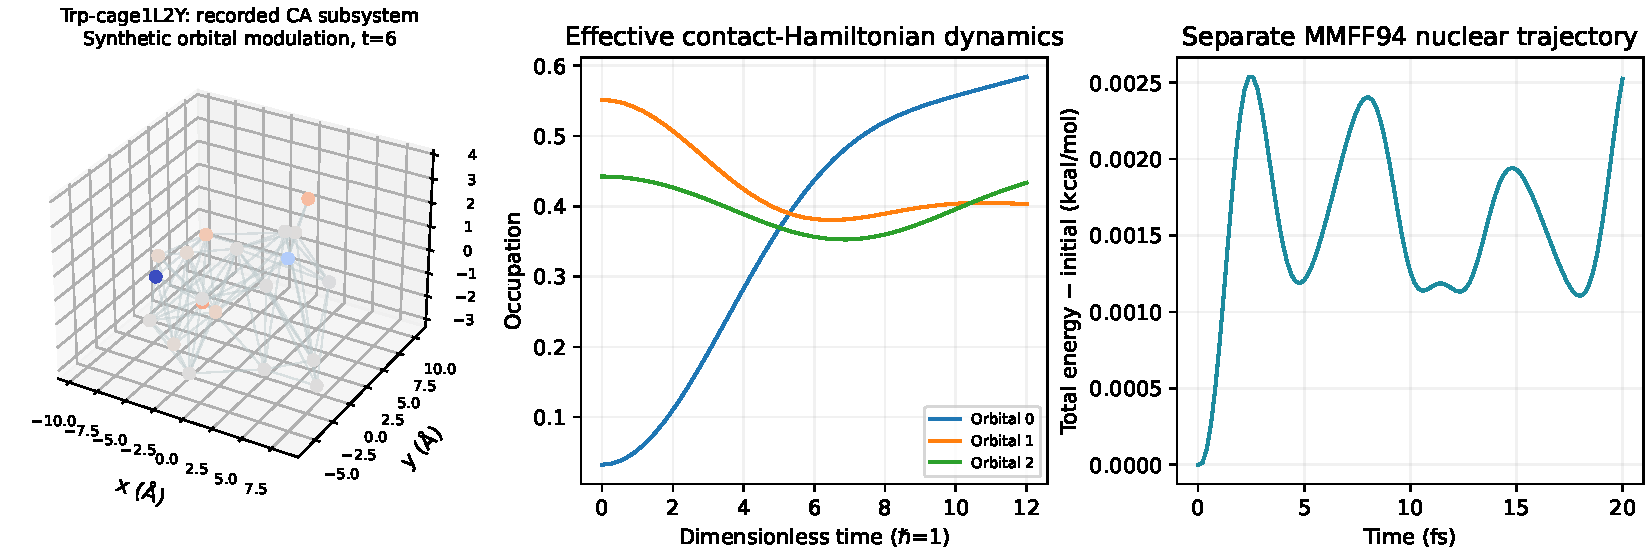
\includegraphics[width=\textwidth]{figures/complementary-datasets.pdf}
\caption{Actual source-backed and computed examples. Left: the recorded Trp-cage
CA subsystem, colored by an uncalibrated contact-model orbital modulation.
Middle: three of its finite orbital occupations. Right: total-energy drift of a
separate explicit-H MMFF94 trajectory. Electronic time and nuclear femtoseconds
are distinct; the contact model is neither an experimental transfer rate nor
an ab-initio density. The interactive tool supplies the actual records and code.}
\end{figure}
\begin{figure}[htbp]
\centering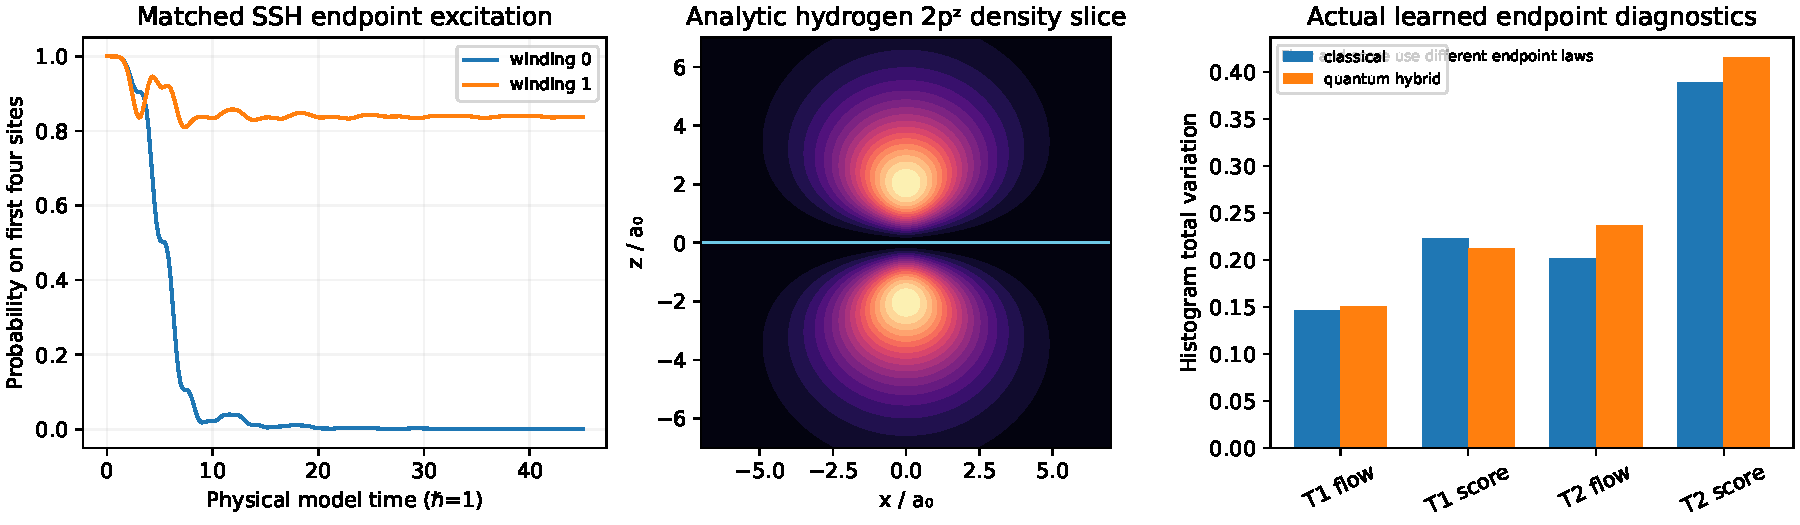
\includegraphics[width=\textwidth]{figures/orbital-flow.pdf}
\caption{Computed matched SSH transport, an analytic hydrogen orbital slice and actual trained chemistry endpoint diagnostics. The diffusion endpoint retains positive heat time; its reference differs from the flow target. These finite results do not establish quantum advantage.}
\end{figure}
\begin{figure}[htbp]
\centering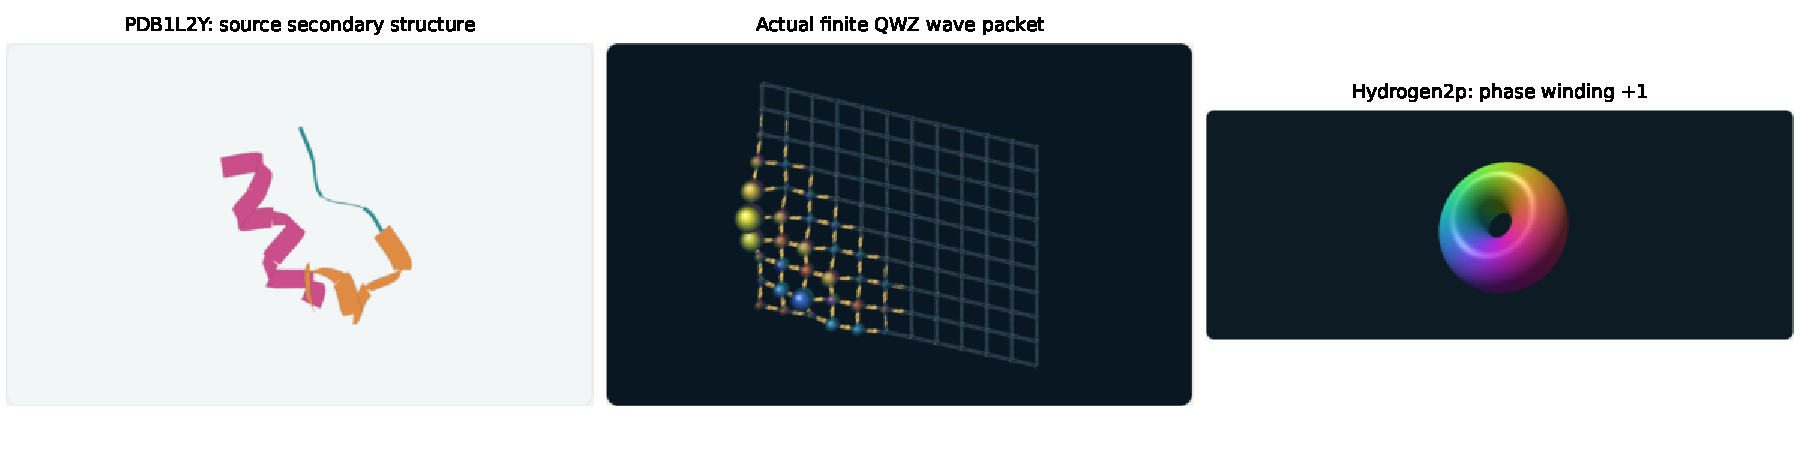
\includegraphics[width=\textwidth]{figures/orbital-atlas.pdf}
\caption{Native interactive renderings: deposited Trp-cage secondary structure, an actual finite QWZ wave packet and an analytic hydrogen phase vortex. Ribbon, probability-height and density-isosurface encodings have different source and physical meanings.}
\end{figure}
% Generated shared reviewed material.
\section{Molecular structure, complex transport and learned chemistry}
The complementary-data laboratory now separates deposited protein structure,
actual finite quantum transport and learned conformation generation. Covalent
bonds use explicit molecular graphs or qualified PDB templates, with depth
ordering and visible atom/bond scales. The ribbon view reads deposited
\texttt{HELIX}/\texttt{SHEET} records; short synthetic peptide backbones remain
unassigned rather than acquiring invented secondary structure.

Five additional finite propagation examples compare matched SSH/QWZ
topological and trivial controls and an SSH domain wall. Complex phase,
probability, current, coherence and selected eigenstates are distinct views.
Analytic hydrogen volumes illustrate nodes, quantum beats and a phase vortex;
they are not molecular electronic-structure calculations. Eight further CPU
runs train classical and two-qubit hybrid score/flow models on periodic MMFF
butane/pentane torsion spaces. All checkpoints, losses, controls and positive
noise endpoints are explicit. These examples neither establish quantum
advantage nor close the independent arithmetic bridge for GRH.

% Generated shared reviewed material.
\section{Geometry, orbitals and generative time}
\subsection{Chemical connectivity and source secondary structure}
An atomic coordinate cloud does not determine chemical bonds merely by
looking connected. SDF graphs retain their explicit bond indices. For the PDB
source view we select the first model, blank/A alternate locations and positive
occupancy; solvent is omitted from the display. Standard amino-acid templates,
explicit \texttt{CONECT}, qualified ligand/hydrogen proximity and geometrically
valid peptide C--N links have separate provenance. The complete original file
remains available. Display connectivity is not a newly measured bond label.

The parser follows the wwPDB3.3 record definitions \cite{VisPDB}. A class-one
\texttt{HELIX} is an alpha helix; class five is a $3_{10}$ helix, not another
alpha helix. \texttt{SHEET} retains strand identity, sheet membership and
parallel/antiparallel sense. Ribbon patches follow the actual CA trace and
carbonyl orientation, with strand arrows and narrower coils. A peptide bond
must connect neighboring residues before a patch or spline-control neighbor
is allowed: spatially nearby disconnected fragments and TER-separated chains
must not acquire a phantom ribbon. Regression tests include these controls.
Backbone recognition in a short synthetic SDF peptide supplies a trace, not a
DSSP assignment or evidence of a stable secondary structure.

The full-source geometry is distinct from the capped effective contact graph.
In the full-source view, only mapped modeled CA sites carry its electronic
field. Nuclear display interpolation adds no new integration steps. An NMR
model index, a ribbon parameter and a generative time are not physical time.

\subsection{What the complex transport animation computes}
For a finite Hermitian matrix $H=V\operatorname{diag}(E_k)V^*$ and a normalized
initial vector $\psi_0$, the continuously evaluated browser state is
\[
 \psi_j(t)=\sum_k V_{jk}e^{-itE_k}(V^*\psi_0)_k.
\]
Unitarity gives $\sum_j|\psi_j(t)|^2=1$. Differentiating gives
$\dot n_i=2\operatorname{Im}\sum_jH_{ij}\psi_j\bar\psi_i$ and hence
$\dot n_i+\sum_jJ_{ij}=0$ for
$J_{ij}=-2\operatorname{Im}(H_{ij}\psi_j\bar\psi_i)$.
The actual complex one-particle coherence is
$\rho_{ij}=\psi_i\bar\psi_j$. A common phase cancels from both current and
coherence; node colors therefore use a stated phase reference. The probability
height is a display encoding, not another physical coordinate. Current arrows
are fluxes, not classical electron paths.

Two48-site SSH controls use the same initial endpoint orbital and exchanged
strong/weak hoppings. Their periodic bulk winding is respectively zero and
one for $q(k)=t_1+t_2e^{ik}$, with gap $2|t_1-t_2|$. A separate61-site domain-wall chain starts and ends
with strong bonds and has two weak bonds adjacent to its central even site.
Its sublattices have sizes31 and30. At zero energy, set the odd-site amplitudes
to zero and solve the tridiagonal recurrence on even sites. The amplitudes
decay away from the wall by the weak/strong ratio. The nonzero off-diagonal
entries determine this vector up to scale, so the nullspace is one-dimensional.
This proves a finite interface zero mode; it does not identify an arithmetic
Hilbert--P\'olya spectrum.

The QWZ examples have a $12\times10$ rectangle and two orbitals per site.
They use the same unfiltered corner spinor for masses $-1$ and $-3$.
Their bulk Chern numbers are $-1$ and0 in the existing link-product convention;
32/64 meshes and gauge controls agree. Finite boundary probability, spectral
weights and coherence remain measurements of the particular finite state,
not definitions or proofs of that bulk invariant. Independent matrix-exponential
checks reproduce the five propagated states. The hydrogen phase winding below,
chemical torsion torus, dessin genus and persistent-homology classes are also
different invariants.

\subsection{An analytic orbital benchmark with actual nodes}
In atomic units, take $h=-\frac12\Delta-r^{-1}$ on the usual hydrogen domain.
The displayed normalized eigenfunctions are
\[
 \phi_{1s}=\pi^{-1/2}e^{-r},\qquad
 \phi_{2s}=\frac{(2-r)e^{-r/2}}{4\sqrt{2\pi}},\qquad
 \phi_{2p_j}=\frac{x_j e^{-r/2}}{4\sqrt{2\pi}}.
\]
Their energies are $E_1=-1/2$, $E_2=-1/8$. The angular integrals and
$\int_0^\infty r^n e^{-ar}\,dr=n!a^{-n-1}$ give their unit norms;
opposite angular parity gives orthogonality of $1s$ and $2p_z$.
Consequently
\[
 \psi(t)=\sqrt{1-a}\,\phi_{1s}
       +\sqrt a\,e^{-3it/8}\phi_{2p_z},\qquad 0\le a\le1,
\]
has unit norm after removing its unobservable common ground-state phase.
Its density has the interference term
$2\sqrt{a(1-a)}\phi_{1s}\phi_{2p_z}\cos(3t/8)$: this is the actual quantum
beat shown in the volume. The $2s$ radial node is $r=2$; the $2p_z$ nodal
plane is $z=0$.

The state $(\phi_{2p_x}+i\phi_{2p_y})/\sqrt2$ is proportional to
$(x+iy)e^{-r/2}$. On a circle avoiding the nodal axis its phase winds once,
and $L_z\psi=\psi$. Its current is
$\operatorname{Im}(\bar\psi\nabla\psi)$ and has an azimuthal component.
This stationary density with nonzero current need not show a moving classical
particle. A finite-radius ray-marched volume and its opacity/exposure curve
are rendering choices, distinct from the analytic density and normalization.
These are nonrelativistic isolated-hydrogen benchmarks, not many-electron
molecular orbitals or ab-initio peptide density.

\subsection{A useful periodic chemical target}
Butane has one selected torsion; pentane has two. All other internal coordinates
are held at the recorded MMFF reference geometry. The finite grids have72 and
$24^2$ points, respectively. At300K define
\[
 p_k=Z^{-1}\exp[-(E_k-E_{\min})/(k_BT)],\qquad
 q_0(\theta)=\sum_k p_k\,K_{\sigma^2/2}(\theta-\theta_k),\quad \sigma=.05,
\]
where the product wrapped heat kernel is used on $\mathbb T^d$ and $d=1,2$.
Thus $q_0$ is an explicitly softened finite-grid Gibbs target. It is positive,
smooth and normalized; it is not a full solvent or molecular-equilibrium
distribution. No affinity, redox, efficacy or electronic-density label is inferred.
The molecular animation rotates downstream atoms about each actual bond axis;
its poses agree with independent RDKit dihedral assignments to numerical
precision and preserve the bond graph and fixed bond lengths.

\subsection{Score diffusion on the torus}
For the unit circle,
\[
 K_\tau(x)=\sum_{m\in\mathbb Z}\frac{e^{-(x+2\pi m)^2/(4\tau)}}{\sqrt{4\pi\tau}},
 \qquad \partial_\tau K_\tau=\partial_x^2K_\tau.
\]
The product kernel gives $q_\tau=q_0*K_\tau$ and
$\partial_\tau q_\tau=\Delta q_\tau$. A forward sample is
$X_\tau=\operatorname{wrap}(X_0+\sqrt{2\tau}\,\xi)$.
Conditioning the wrapped Gaussian mixture shows
\[
 \nabla\log q_\tau(x)
 =\mathbb E[-\xi/\sqrt{2\tau}\mid X_\tau=x].
\]
Indeed, differentiate each image term and divide by the mixture density;
the Gaussian score is the stated latent-noise target. Conditional least
squares therefore identifies the marginal score. The implemented weighted
DSM loss uses weight $2\tau$, not an unlabelled Euclidean proxy on cut angles.
The periodic-input network is trained over the full normalized time interval.

With reverse clock $u$, the ideal SDE is
$dY_u=2\nabla\log q_{T-u}(Y_u)\,du+\sqrt2\,dW_u$.
Its Fokker--Planck equation at density $q_{T-u}$ is
$-2\Delta q+\Delta q=-\Delta q$, as required. This connection to score SDEs
is the standard method \cite{VisScore}; the periodic mixture here supplies an
explicit control. Initialization is sampled from the actual $q_T$, with $T=2$,
rather than silently assuming it is uniform. Sampling stops at $\tau=.03$,
so the ideal endpoint is $q_{.03}$, whose Gaussian component variance is
$\sigma^2+.06$. It is not $q_0$. The initial run exposed this distinction;
its source and outputs are preserved. The corrected run uses the proper endpoint
reference and no excluded small-time training interval.

Exact wrapped-mixture scores, finite-difference checks, nested64/128-step
Brownian controls and stored learned trajectories accompany the experiment.
A finite Euler diagnostic is neither a convergence theorem nor a guarantee
that a learned score recovers equilibrium. Remaining noise and learned-field
error are shown separately from the MMFF target.

\subsection{Wrapped-geodesic flow matching}
Let $X_0$ be uniform on $\mathbb T^d$, independently let $X_1\sim q_0$, put
$D=\operatorname{wrap}(X_1-X_0)$ and
$X_t=\operatorname{wrap}(X_0+tD)$. The cut locus has probability zero under
these continuous laws. For every smooth periodic test function $f$,
\[
 \frac d{dt}\mathbb Ef(X_t)
 =\mathbb E\langle\nabla f(X_t),D\rangle
 =\int\langle\nabla f(x),v_t(x)\rangle\rho_t(x)\,dx,
 \quad v_t(x)=\mathbb E[D\mid X_t=x].
\]
This is the weak continuity equation with the correct uniform and $q_0$
endpoints. Writing $B=[-\pi,\pi]^d$, the conditional formulas are explicitly
\[
 \begin{aligned}
 \rho_t(x)&=(2\pi)^{-d}\int_Bq_0(x+(1-t)D)\,dD,\\
 \rho_t(x)v_t(x)&=(2\pi)^{-d}\int_BD\,q_0(x+(1-t)D)\,dD.
 \end{aligned}
\]
Because $q_0$ is smooth and strictly positive on the compact torus,
these integrals are jointly smooth through both endpoints and
$\rho_t\ge\min q_0>0$. Division gives a smooth bounded periodic $v_t$
with a uniform spatial Lipschitz bound. In particular $v_1=0$ by symmetry. The usual unique flow of this globally Lipschitz
time-dependent field transports the stated marginals. Conditional regression
targets $D$ and learns an approximation to $v_t$, following the flow-matching
and manifold formulation \cite{VisFlow,VisRFM}. Neither the regression loss
nor a visualization replaces endpoint-error measurement.

\subsection{Physical state preparation, RG and phase-conditioned design}
The earlier seven-spin dessin experiment supplies an actual quantum Gibbs
state and its partial trace; its learned circuits approximate specified
state/field targets. The exact coarse action in the RG chapter is produced
by integrating out physical spins. Here the chemical learner transports a
classical probability law on internal coordinates. A quantum channel, an RG
partial trace and a score/noise schedule are three different constructions,
with different states, clocks and acceptance tests.

A concrete materials-design constraint already appears in the QWZ controls.
Any continuous mass path from $m=-3$ to $m=-1$ passes through $m=-2$.
The explicit bulk gap formula then gives zero gap. Thus such a generator
cannot both change between these two Chern sectors and preserve the gap
throughout that path. Sector-conditioned sampling, explicit transition
states and gap/invariant checks are meaningful design tasks. Merely drawing
a continuous latent interpolation does not meet them. The finite transport
controls and the earlier learned thermal-state experiments provide distinct
physics benchmarks for these requirements, rather than unverified
predictions of a synthesized topological material.

\subsection{What the quantum hybrid actually contributes}
Each hybrid has two re-uploading two-qubit layers: periodic $R_z$ angle/time
encoding, trainable $R_y$ rotations and CZ, followed by eight actual Pauli
expectations and a two-layer64-unit tanh classical readout. The angles and
readout are trained together. Integer coordinate frequencies preserve
$2\pi$ periodicity of the measured features, and composition preserves it in
the vector field. These are classically simulated quantum-feature hybrids,
not coherent quantum chemical evolution or quantum-assisted measurements.
The matched classical controls use periodic first/second harmonics and the
same readout width. Parameter counts and individual seeds remain explicit.

Eight2400-update CPU runs retain heldout objectives, checkpoint weights,
periodicity errors, independent Kronecker/Pauli calculations, parameter
finite differences, exact-score comparisons and actual endpoint histograms.
The limited runs do not establish quantum advantage. Flow and diffusion have
different positive-noise endpoint laws and must not be ranked as though their
targets were identical. Generative interpolation time is not molecular time.

The chemical torus is a concrete internal-coordinate space. Drawing it next
to a dessin, a noncommutative torus or a Fukaya construction does not construct
a functor or prove homological mirror symmetry. Likewise none of these finite
learners constructs the missing arithmetic self-adjoint determinant bridge.
Adding heat/noise is also distinct from integrating out physical degrees of
freedom in the earlier actual RG chapter; a noise schedule alone is not an RG
construction. New source, operator-domain, arithmetic and Lean obligations remain explicit.

\IfFileExists{chapters/dataset-release-links.tex}{\section{Public release access}
Both datasets are additional public Parquet releases, with dataset cards,
origin columns, source records, audit evidence and exact remote hashes.
\paragraph{Aster complementary topological response}\href{https://huggingface.co/datasets/AmelieSchreiber/GRH-Aster-TopoResponse-20261104}{Public Hugging Face dataset}.\\
Default static rows: 16,384; separately labelled source-anchor rows: 576.\\
Verified dataset commit: \texttt{2b8ce36571298a3517b8c88bb23269341d9b8908}.\\
\paragraph{Mora complementary conformer response}\href{https://huggingface.co/datasets/AmelieSchreiber/GRH-Mora-ConformerResponse-20261104}{Public Hugging Face dataset}.\\
Default static rows: 22,951; separately labelled source-anchor rows: 266.\\
Verified dataset commit: \texttt{53a6b66acaa69ef79584648f3f6dc068363c4837}.\\
Use the pinned commit and configuration names from the dataset card; time
frames do not count as independent systems. The interactive explorer retains
the full release receipts and actual source-file downloads. No dataset was
enrolled into either active model during this work.

The data commits above remain immutable. Public visibility was enabled at the
owner's request on 4 November 2026, with new card-only commits recorded in
\texttt{outputs/publication/2026-11-04}. No data file changed.
}{}

% Generated shared reviewed material.
\section{Coherent electron-density clouds in an explicit spatial basis}
The density viewer now evolves spatial functions, including interference
terms, instead of drawing independent spheres around occupied sites. Let
$g_i(\mathbf r)$ be normalized real Gaussian basis functions, let
$S_{ij}=\int g_i g_j$ be their positive-definite overlap, and set
$L=S^{-1/2}$. For a Hermitian orthonormal-basis Hamiltonian $h$ and a matrix
$C_0$ of $p$ orthonormal occupied columns, put
\[
 C(t)=e^{-ith}C_0,\qquad
 \rho(\mathbf r,t)=\sum_{a=1}^p
       \left|\sum_i g_i(\mathbf r)(LC(t))_{ia}\right|^2.
\]
This density is nonnegative and has integral $p$: unitarity preserves
$C(t)^*C(t)=I$, and integration yields
$\operatorname{Tr}(C(t)^*L^*SL C(t))=p$. The cross terms carry coherence.
Replacing them by a sum of atomic densities generally changes the model.
The displayed gain/loss field is $\rho(t)-\rho(0)$, whose full-space integral
is zero; positive and negative colors indicate redistribution, not particles
with negative probability. Time interpolation of saved density frames is a
display operation and is not an extra time-integration step.

For fixed-nuclei $\mathrm H_2^+$ at separation $2a_0$, six normalized $s$
Gaussians (exponents $0.3,1.2,4.8$ at each nucleus) give an explicitly
integrated one-electron Coulomb Galerkin model. We start in one normalized
left-center Gaussian, then evolve with its time-independent Hamiltonian.
The electronic ground energy is approximately $-1.08675615$ Hartree;
adding nuclear repulsion gives $-0.58675615$ Hartree. This small basis is not
a chemical-accuracy or basis-convergence result. Independent Coulomb
quadrature, kinetic-integral and matrix-exponential checks pass.

The second example uses the deposited Trp-cage CA geometry, a specified
twenty-orbital contact Hamiltonian and ten occupied model orbitals. Its
spatial Gaussians have exponent $0.25\,\text{\AA}^{-2}$. The resulting field
is the exact density of this finite effective basis model, not a calibrated
protein electron density, valence count or transfer-time prediction.
The first example uses atomic units; the second retains its effective model
time and length convention. These examples are separate from the fixed
private dataset release and do not change its labels.

The viewer offers orbit/zoom, volume and isosurface rendering, time scrubbing,
exposure and density/gain-loss palettes. The $64^3$ grid and 41 saved frames
are encoded as 8-bit square-root-density atlases. The maximum decoded
integrated-charge errors are $0.00158$ electron for $\mathrm H_2^+$ and
$0.00141$ model particle for Trp-cage; analytical full-space charge
conservation is exact. Rendering thresholds, finite boxes and quantization
are explicit display limitations. The separate hydrogen viewer retains exact
analytic hydrogen orbitals and their coherent time-dependent superpositions.


\chapter[ToricGT and mirror interfaces]{ToricGT: quantum features, tropical certificates and mirror interfaces}
\label{tg:chapter}

ToricGT organizes graph tokens, trajectories and auxiliary algebraic data; its
companion research program separates architecture, dynamics, memory, oracle
labels and toric training objectives \cite{TGTCode,TGTProgram}. This chapter
extends that organization to the present surface-order problem. A quantum
feature map can replace a specified finite feature block, and exact algebra
can check a proposed relation or parameter. Neither operation supplies the
arithmetic identification needed by Hilbert--P\'olya.

The inspected ToricGT revision is
\texttt{a5199bc989a6fb170e21220e5e87bf95bc2fc0b4}; the program revision is
\texttt{f91ba1811b5a4f70d53c7120acf8ca2a0049f85b}.
The files \texttt{toric\_algebra.py},
\texttt{tropical\_toric\_certificates.py},
\texttt{cas\_certificates.py} and the graph-token schemas are the concrete
interfaces used here. Their mathematical objects are not inferred from
repository names. In particular, we do not claim to have reproduced the
upstream language-model training campaigns or their compression scores.

\section{A toric chart inside an actual dessin representation stratum}
Let $A$ be the infinite polynomial elliptic-square dessin algebra of the
preceding chapters. It has two quiver vertices, two arrows in each direction,
and the specified locally gentle zero relations. Retain one arrow
$X:V_0\to V_1$, put the other arrows equal to zero, and frame
$V_0=V_1=k^2$. Every path of length two now acts by zero, so these are genuine
continuous finite-dimensional modules of the completed order as well.
Impose the additional closed condition $\operatorname{rank}X\leq1$.
In the chosen frames write
\[
 X=\begin{pmatrix}z_{00}&z_{01}\\z_{10}&z_{11}\end{pmatrix},\qquad
 f=z_{00}z_{11}-z_{10}z_{01}.
\]
The coordinate ring is $B=k[z_{00},z_{01},z_{10},z_{11}]/(f)$.
This is a representation \emph{stratum with a rank condition}; it is not an
assertion that the full order or its invariant ring is a toric variety.

\begin{proposition}[The Segre semigroup and its full relation]\label{tg:segre}
The homomorphism
\[
 \begin{split}
 \pi:k[z_{00},z_{10},z_{01},z_{11}]&\longrightarrow k[s,x,y],\\
 z_{ij}&\longmapsto sx^iy^j
 \end{split}
\]
has kernel $(f)$. Its image is the semigroup ring generated by
$(1,0,0),(1,1,0),(1,0,1),(1,1,1)$ in $\Z^3$.
With all $z$ of degree one,
\[
 H_B(t)=\frac{1-t^2}{(1-t)^4}
       =\frac{1+t}{(1-t)^3},\qquad \dim_kB_n=(n+1)^2.
\]
\end{proposition}
\begin{proof}
The displayed binomial maps to zero. Replace any factor $z_{00}z_{11}$
in a monomial by $z_{10}z_{01}$ until no such factor remains. The integer
kernel of the exponent matrix is generated by $(1,-1,-1,1)$ in the
order $(00,10,01,11)$. Two distinct reduced monomials cannot have the same
image: their exponent difference would be a nonzero multiple of this
vector, and the monomial at the positive end would contain both
$z_{00}$ and $z_{11}$. Distinct reduced monomials therefore have linearly
independent images. Reducing a polynomial proves $\ker\pi=(f)$.
Multiplication by $f$ is injective in the polynomial domain $P=k[z]$,
so the graded exact sequence
$0\to P(-2)\xrightarrow{f}P\to B\to0$ gives the Hilbert series.
In degree $n$, image monomials are exactly $s^nx^ay^b$ with
$0\leq a,b\leq n$: choose the overlap of the $a$ $x$-positions and
$b$ $y$-positions between $\max(0,a+b-n)$ and $\min(a,b)$.
This gives $(n+1)^2$ monomials.
\end{proof}

This supplies a small complete certificate rather than an unspecified
``syzygy loss.'' A learned output $\widehat z$ can be penalized by
$|f(\widehat z)|^2$. After rationalization, checking $f(z)=0$ exactly
certifies the rank-one relation. It does not certify the learned point's
interpretation as a module with other nonzero arrows, an arithmetic
endomorphism, or a positive spectral family. The multiplicative
parametrization $z_{ij}=a_i b_j$ enforces this one relation identically,
including degenerate rank-zero points.

The projectivization of this cone is the Segre surface
$\mathbb P^1\times\mathbb P^1$. The full framed representation space,
the rank-one cone, its projectivization and a quotient by the vertex group
are different objects. Under the full left-right action on $X$, its
individual entries are not all semi-invariants. The determinant has its
usual determinant character, but is identically zero on this stratum.
Framing is thus part of the example, not an invisible choice of gauge.

\section{Tropical charts and exactly what their certificates prove}
The same square of exponents defines the max-plus function
\[
 \psi(u,v)=\max\{0,u,v,u+v\}=\max\{0,u\}+\max\{0,v\}.
\]
Its corner locus is the union of the coordinate axes. There are four
one-dimensional rays of weight one, with primitive outgoing directions
$(1,0),(-1,0),(0,1),(0,-1)$. Their sum is zero. This is an exact local
balancing calculation. The Newton polygon is the unit square.

\begin{center}
\begin{tikzpicture}[scale=1.15,>=Stealth]
 \draw[->,gray] (-2,0)--(2.1,0) node[right]{$u$};
 \draw[->,gray] (0,-1.7)--(0,1.7) node[above]{$v$};
 \draw[very thick,teal!70!black] (-1.6,0)--(1.6,0);
 \draw[very thick,teal!70!black] (0,-1.3)--(0,1.3);
 \fill (0,0) circle (2pt);
 \node at (1,.8) {$u+v$};\node at (-1,.8) {$v$};
 \node at (1,-.8) {$u$};\node at (-1,-.8) {$0$};
 \node[align=center] at (0,-2.1) {Four rays, weight one\\local balance $=0$};
 \begin{scope}[xshift=5.4cm]
  \draw[thick] (0,0)--(1.5,0)--(1.5,1.5)--(0,1.5)--cycle;
  \foreach \x/\y/\lab in {0/0/00,1.5/0/10,0/1.5/01,1.5/1.5/11}
   {\fill (\x,\y) circle (2pt);\node[above right] at (\x,\y) {$a_{\lab}$};}
  \node[align=center] at (.75,-1.1) {Dual Newton square\\$a_{00}+a_{11}=a_{10}+a_{01}$};
 \end{scope}
\end{tikzpicture}
\end{center}

There are two associated tropical constructions, and they should not be
conflated. The hypersurface of a four-term polynomial with this support
lives in $\R^2$. The tropicalization of the two-term Segre ideal lives in
$\R^4$ and satisfies
\[
 w_{00}+w_{11}=w_{10}+w_{01}.
\]
The latter follows because the two terms of the binomial must have equal
valuation. Over a valued field, tropicalization records valuations and
initial degenerations; it is not a literal embedding of the tropical
set as an ordinary algebraic subvariety of the complex toric variety.
A fan specifies a toric compactification, while compatibility with that
fan and the valued-field data specifies the relevant tropical geometry.

The inspected helper in \texttt{tropical\_toric\_certificates.py} uses
integer supports, rational wall intersections and polygon edge normals.
At this revision its input conversion applies \texttt{int} to floats.
Consequently the exact claim here is restricted to inputs already
verified to be integral; a nonintegral learned exponent cannot be silently
rounded into an exact certificate. Pairwise ties also need their dimension
checked. In the square example the pair $(00,11)$ ties maximally only at
the origin, as does $(10,01)$. These zero-dimensional sets are not extra
facets. A balancing sum for one dual polygon is not by itself a certified
Chow class on an unspecified complete fan, nor an exact description of a
higher-dimensional tropical variety. The stronger boolean names in the
upstream record are not used as additional mathematical premises here.

A useful hybrid pipeline learns affine scores with real parameters,
exports integer/rational candidates with an explicit approximation rule,
and then recomputes active cells, dimensions, weights and balancing
exactly. The approximation error belongs to the learned model; the
certificate belongs to the exported data. Recording both prevents a
small floating residual from becoming an alleged exact identity.

\section{The quantum phase block and its cocycle}
The ToricGT shift convention differs from the forward shift used in some
other chapters. At $\theta=p/q$, with $\omega=e^{2\pi i\theta}$, its
untwisted matrices act by
\[
 Ue_j=\omega^je_j,\qquad Ve_j=e_{j-1\bmod q},\qquad
 VU=\omega UV.
\]
If $p,q$ are coprime they are a finite irreducible carrier of a central
quotient. They do not faithfully represent the full rational rotation
algebra. A boundary twist has to have modulus one if $V$ is to be
unitary. Rational approximants to an irrational $\theta$ produce a
sequence of finite models, but not an automatically nested sequence of
matrix-algebra inclusions.

\begin{proposition}[Ordered and symmetric Weyl multipliers]\label{tg:cocycle}
For integer pairs $x=(a,b)$ and $y=(c,d)$ set
$W(x)=U^aV^b$. Then
\[
 W(x)W(y)=\omega^{bc}W(x+y).
\]
Choose a real lift of $\theta$ and set
$D(a,b)=e^{\pi i\theta ab}U^aV^b$. Then
\[
 D(x)D(y)=e^{\pi i\theta(bc-ad)}D(x+y),\qquad
 D(x)D(y)=e^{2\pi i\theta(bc-ad)}D(y)D(x).
\]
These formulas are on $\Z^2$; descent to exponents modulo $q$ requires
retaining the resulting central phases.
\end{proposition}
\begin{proof}
Repeated use of $VU=\omega UV$, including inverses, gives
$V^bU^c=\omega^{bc}U^cV^b$ and proves the first identity.
The exponent introduced by the symmetric gauge is
\[
 \tfrac12ab+\tfrac12cd+bc-\tfrac12(a+c)(b+d)
 =\tfrac12(bc-ad).
\]
Reversing $x,y$ negates this last expression. Dividing the two multipliers
proves the commutator formula. Associativity also follows directly from
bilinearity: $bc+(b+d)e=de+b(c+e)$ for a third pair $(e,f)$.
\end{proof}

The generic routine \texttt{projective\_phase} instead evaluates
$\exp(2\pi i x^T\Theta y)$. For skew $\Theta$ its commutator phase
is $\exp(4\pi i x^T\Theta y)$. To match the preceding symmetric gauge,
use the explicit matrix
\[
 \Theta=\begin{pmatrix}0&-\theta/2\\\theta/2&0\end{pmatrix}.
\]
This factor of two and the orientation sign matter for learned phase
features, circuit comparisons and transport around a surface. A separate
numerical skew matrix is not automatically the ordered multiplier
$\omega^{bc}$. For even $q$, writing $1/2$ modulo $q$ would introduce
another error; the real-lift formula avoids that operation.

For a density matrix $\rho$, one physically measurable feature is
\[
 f_x(\rho)=\operatorname{Tr}(\rho D(x)).
\]
Its real and imaginary parts are expectations of the Hermitian operators
$(D(x)+D(x)^*)/2$ and $(D(x)-D(x)^*)/(2i)$. They lie in $[-1,1]$.
Thus a classical graph-token block can receive measured finite-dimensional
phase features; a variational circuit can learn the state preparation or
bounded observables; and a classical head can combine these with exact
combinatorial records. No claim of quantum speedup follows from replacing
an already inexpensive matrix calculation by a circuit.

\begin{proposition}[A genuine positive feature kernel]\label{tg:kernel}
For any finite list $x_i$ and any density matrix $\rho$, the matrix
$K_{ij}=\operatorname{Tr}(\rho D(x_i)^*D(x_j))$ is positive semidefinite.
\end{proposition}
\begin{proof}
For complex $c_i$ put $B=\sum_i c_iD(x_i)$. Then
$\sum_{ij}\overline c_iK_{ij}c_j=\operatorname{Tr}(\rho B^*B)
=\operatorname{Tr}((B\sqrt\rho)^*B\sqrt\rho)\geq0$.
\end{proof}
This proof applies to a physical Gram kernel. It does not identify that
kernel with a Jensen metric, the arithmetic explicit-formula pairing, or
the determinant family of a completed $L$-function. The latter comparison
is an additional theorem, not a consequence of positivity of $\rho$.

\section{A quantum--classical ToricGT extension with auditable interfaces}
A typed record for a surface example should contain dart permutations,
arrow endpoints, zero relations, central parameters, coefficient fields,
module dimensions and category labels. Neural embeddings can be added to
these records; they should not replace them. A candidate hybrid block is
\[
 h_v' = F_\eta\!\left(h_v,\sum_{w\sim v}\alpha_{vw}h_w,
      \{\Re f_x(\rho_v),\Im f_x(\rho_v)\}_x,\;c_v\right),
\]
where $\alpha$ is a normalized classical attention rule, $\rho_v$ is
prepared by a specified finite circuit, and $c_v$ is an exact certificate
summary. Its architecture is meaningful even if the quantum features are
first simulated classically, as in the finite training examples of the
preceding computational chapter.

\begin{center}
\begin{tikzpicture}[>=Stealth,node distance=7mm,
 box/.style={draw,rounded corners,align=center,font=\small,text width=38mm,minimum height=13mm}]
 \node[box] (data) {Dessin and\\ module records};
 \node[box,right=of data] (learn) {Graph tokens\\ quantum features};
 \node[box,right=of learn] (proposal) {Candidate maps\\ metrics and parameters};
 \node[box,below=of proposal] (check) {Exact algebra\\ and proof checker};
 \node[box,left=of check] (ledger) {Verified result\\ or failed step};
 \draw[->] (data)--(learn);\draw[->] (learn)--(proposal);
 \draw[->] (proposal)--(check);\draw[->] (check)--(ledger);
 \draw[->] (ledger.west)-| (data.south);
\end{tikzpicture}
\end{center}

There are three distinct uses. First, supervised regression can learn a
coarse-graining map against exact Ising or Gaussian targets, with a held-out
parameter set. Second, a proposal model can search for a small module map
or a polynomial identity, checked by exact substitution and stated
presentation relations. Third, a proof-search policy can select candidate
lemmas or tactics, whose accepted output must pass the proof assistant.
Only the last two have the potential to yield new exact mathematical
results, and only when the checker verifies the full exported statement.
A classifier predicting that a proof is valid is not such a checker.

The ToricGT program's certificate distinction is particularly useful here:
store exact CAS data, validated surrogates and unavailable backends as
different provenance classes. When comparing a quantum feature head with
a classical one, hold the data split, parameter budget and objective fixed;
report sample or simulation cost as well as error. A network with extra
features need not improve the objective. None of the finite experiments
in this book is an upstream full-transformer language-model ablation.

An exact candidate metric $G$ for a finite matrix $M$ illustrates the
proposal/check distinction. For rational real entries, symmetry and all
principal-minor nonnegativity can certify $G\succeq0$. Positive
definiteness and $GM=M^*G$ then imply similarity to a Hermitian matrix:
$G^{1/2}MG^{-1/2}$ is Hermitian. Checking a few sampled minors or a small
floating residual does not prove these assertions, and applying the result
to an arithmetic family still requires uniform positivity and the exact
arithmetic determinant comparison.

\section{Mirror symmetry supplies category comparisons, not a spectral shortcut}
Kontsevich--Soibelman develop torus-fibration and homological-perturbation
methods, including an $A_\infty$ comparison for specified subcategories of
abelian mirrors \cite[Sections 6--8, Theorem 4]{TGKontsevichSoibelman}.
A lattice of phase labels is useful computational data for such geometry,
but a finite Weyl pair alone does not construct either Fukaya objects or
an $A_\infty$ functor. The latter must carry complexes of morphisms and
all higher composition maps with their signs and convergence rules.

A concrete toric theorem provides a better model for the proposed link.
For a smooth projective toric $X$, Abouzaid constructs a full
$A_\infty$ sub-pre-category of the relative Fukaya category of its
Landau--Ginzburg mirror that is quasi-equivalent to the DG category of
line bundles on $X$ \cite[Theorem 1.2 and Corollary 1.4]{TGAbouzaid}.
The theorem gives an embedding after the indicated derived/split closure;
it does not assert an unrestricted equivalence for every non-Fano toric
variety or for our singular completed order.

For intuition, the customary toric mirror potential for the Segre surface
is
\[
 W(z,w)=z+z^{-1}+w+w^{-1},\qquad (z,w)\in(\C^*)^2.
\]
Solving $z\partial_zW=w\partial_wW=0$ gives
$(z,w)=(\pm1,\pm1)$, with critical values $4,0,0,-4$.
The logarithmic Hessian is diagonal with entries $z+z^{-1}$ and
$w+w^{-1}$ and is nonsingular at those four points. This is a direct
calculation of a mirror \emph{potential}. By contrast the two-level clock
matrix $2Z+2X$ has eigenvalues $\pm2\sqrt2$, since $XZ+ZX=0$.
The critical values and matrix eigenvalues are plainly different data.
A proposal to relate them must specify a functor or quantization and its
normalization; visual resemblance of their torus coordinates is not that
comparison.

For gentle surfaces, the precise positive input already used in this
book is the equivalence for a homologically smooth graded locally gentle
algebra with its prescribed stopped surface and line field
\cite[Theorem 3.2.2]{LekiliPolishchuk}. Our nonempty closed dessin algebras
have forbidden cycles and fail that smoothness hypothesis. A stopped
quotient or categorical resolution can be a meaningful intermediate
object, but it requires its own functor. Ordinary exact quotient
inflation does not automatically preserve derived Hom spaces, AR
triangles or determinants. In particular, the polynomial node branch
$k[x]$ has a valid stopped-annulus interpretation, whereas inflation into
$k[x,y]/(xy)$ is not derived fully faithful, as proved earlier.

A finite training loss for $m_1^2=0$ or a chain-map residual checks only
the displayed truncation. A genuine category construction additionally
needs the remaining $A_\infty$ equations, admissible geometric objects,
grading, compactness or convergence, and the claimed generation result.
Tropical gradient trees can guide computations of compositions under
appropriate geometric hypotheses; they do not remove those obligations.
This is a constructive research interface: learn a small candidate,
calculate its maps exactly, and then prove the specified comparison.

\section{What would make the learned component relevant to GRH?}
For the present Hilbert--P\'olya program the useful learned outputs are
candidates for arithmetic correspondences, controlled positive metrics,
coefficient kernels outside the classes already refuted, or estimates
with an exact symbolic witness. Every candidate must be checked against
local Frobenius factors, central and deck actions, determinant
multiplicities, conductor and gamma normalizations, and compact-uniform
convergence on the stated complex domain. A Dirichlet comparison is not
a proof for Hecke or general Artin $L$-functions.

An exact finite witness can disprove a proposed universal construction,
and that is valuable progress. A successful finite fit only proposes its
next theorem. Neither a toric binomial certificate nor a positive quantum
feature kernel proves that all arithmetic approximants have their zeros
on the critical line. The small-gcd analytic estimate and the independent
positive arithmetic determinant comparison therefore remain separate
load-bearing research tasks. The role of the hybrid architecture is to
make their search more explicit, testable and reproducible.

\section{An executed hybrid spectral experiment}
The executable example \texttt{examples/quantum/toricgt\_hybrid.py} imports the pinned ToricGT rotation-algebra module. For $\theta=1/4$ it obtains four-dimensional Weyl generators and forms the Hermitian Harper family
\[
 H_\lambda=U+U^*+\lambda(V+V^*),\qquad 0.1\le\lambda\le1.8.
\]
A two-qubit PennyLane feature circuit and affine head, with twelve parameters, learn the smallest eigenvalue divided by six. Seed 20261104 specifies one hundred sampled couplings, with seventy-five training and twenty-five held-out samples. After 160 Adam updates the held-out mean-square loss is $4.01905\times10^{-5}$, compared with $0.220518$ at initialization. These are finite simulated spectra, not $L$-function zeros.

For six rational test couplings, the program forms the exact rational matrix
\[
 H_\lambda=\operatorname{diag}(2,0,-2,0)+\lambda\operatorname{Adj}(C_4).
\]
It rounds a learned proposal to a rational number $E$ and checks all fifteen nonempty principal minors of $H_\lambda-EI$. A real symmetric matrix is positive semidefinite exactly when every principal minor is nonnegative, so an accepted proposal is an exact lower eigenvalue bound. A rejected proposal is repaired by rational bisection, starting from the independent Gershgorin lower bound $-2-2\lambda$ and the Rayleigh upper bound $-2$. The saved rational minors certify the resulting lower bounds. Thus learning proposes; an independent exact criterion accepts or repairs. The certificate does not depend on the neural prediction being accurate. No arithmetic operator or completed-order equivalence is claimed by this experiment.

This benchmark has an exact closed-form solution: $\det(tI-H_\lambda)=t^2(t^2-4(1+\lambda^2))$, so $E_0=-2\sqrt{1+\lambda^2}$. For $\lambda>0$, rows one and three of $H_\lambda$ agree, and the difference of rows zero and two is $2/\lambda$ times row one. Thus its rank is at most two. Its trace is zero and $\operatorname{tr}(H_\lambda^2)=8(1+\lambda^2)$, giving the stated eigenvalues (and hence characteristic polynomial). The experiment deliberately has an exact oracle: it tests learning, certificate acceptance and repair on a known problem rather than presenting a numerical fit as a new spectral theorem.

\chapter[Persistence and explicit resolutions]{Two-parameter persistence, Schur syzygies and surface-order coefficients}
\label{pers:chapter}
A persistence diagram records how objects and maps change under an ordered
family of inclusions. A projective resolution records the generators,
relations and relations among relations of one module. These descriptions
meet naturally over a polynomial parameter ring. They must still be
distinguished from the infinite locally gentle algebra attached to the
surface: the parameter ring describes the filtration, not a replacement
surface algebra.

The three supplied papers motivate these interfaces
\cite{PersSurfaceI,PersSurfaceII,PersSurvey}. We use their surface-order,
lattice and finite-presentation ideas with the corrections already proved
in this book. In particular, a matrix satisfying consecutive-product zero
is a complex, not automatically a resolution; Fitting base change is not
exact base change; and the existence of a generic resolution is not a
finite terminating algorithm. The worked example below proves its own
exactness and exhibits an actual topological realization.

\section{The polynomial ring encodes the two commuting directions}
Let $k$ be a field and give $\mathbb N^2$ its coordinatewise order. A
persistence module is a covariant functor $P:\mathbb N^2\to\operatorname{Vect}_k$.
Writing $P_{a,b}=P(a,b)$, put
\[
 R=k[x,y],\quad \deg x=(1,0),\quad\deg y=(0,1),\qquad
 \mathcal P=\bigoplus_{a,b\ge0}P_{a,b}.
\]
Multiplication by $x$ and $y$ is the map to the next coordinate in the
corresponding direction. Functoriality makes their square commute.
Conversely the graded pieces and multiplication maps of an
$\mathbb N^2$-graded $R$-module define such a functor. General transition
maps are multiplication by $x^{c-a}y^{d-b}$ when $(a,b)\le(c,d)$.
The exponents are nonnegative in this direction, a useful sign check.

This gives an equivalence for the stated discrete diagrams. Finite
generation is an additional condition, not a consequence of having
finite-dimensional pieces. A module can have infinitely many independent
births. Finite cellular input with finitely many birth grades gives the
finite presentations used here. A real-parameter filtration needs an
appropriate discretization or a different coefficient algebra before
being treated as a module over $k[x,y]$.

We write $R(-a,-b)$ for a free module whose generator has grade $(a,b)$.
Over a field, a finite graded module has a minimal graded free resolution
of length at most two. Minimality means that every differential entry
belongs to $(x,y)$; tensoring with $k=R/(x,y)$ then kills the differentials.
The numbers and grades of the surviving generators are the multigraded
Betti numbers. The field hypothesis matters: $\mathbb Z[x,y]$ has
homological dimension three, and the regular sequence $(2,x,y)$ supplies
a length-three example. The particular resolution below also works
integrally, but that does not make every integral resolution length two.

\section{A complete three-grade example}
Set
\[
 M=R/(x^2,xy,y^2).
\]
Its basis is $1,x,y$, in grades $(0,0),(1,0),(0,1)$. All other graded
pieces vanish. The two nonzero proper transition maps send $1$ to $x$
and $1$ to $y$. In particular, for comparable grades $\nu\le\mu$,
\[
 \rho_M(\nu,\mu)=\operatorname{rank}(M_\nu\to M_\mu)
 =\begin{cases}1&\nu,\mu\in\{(0,0),(1,0),(0,1)\},\\0&\text{otherwise.}\end{cases}
\]
This computes this module's rank invariant; rank invariants do not in
general classify all two-parameter modules.

\begin{figure}[htbp]\centering
\begin{tikzpicture}[>=Stealth,x=1.35cm,y=1.15cm]
\foreach \a in {0,1,2,3}{\foreach \b in {0,1,2,3}{
 \draw[gray!60] (\a,\b) circle (2pt);}}
\foreach \a/\b in {0/0,1/0,0/1}{\fill[teal!70!black] (\a,\b) circle (4pt);}
\draw[->,very thick,teal!70!black] (.09,0)--(.88,0);
\draw[->,very thick,teal!70!black] (0,.09)--(0,.88);
\draw[->,gray] (-.3,-.35)--(3.5,-.35) node[right]{$a$};
\draw[->,gray] (-.35,-.3)--(-.35,3.5) node[above]{$b$};
\node[below] at (0,-.35) {$0$};\node[below] at (1,-.35) {$1$};
\node[left] at (-.35,1) {$1$};
\node[above right] at (0,0) {$1$};\node[above] at (1,0) {$x$};
\node[right] at (0,1) {$y$};
\node[anchor=west,align=left] at (3.9,1.7) {Filled point: one copy of $k$\\Open point: zero\\Only the two thick arrows survive};
\end{tikzpicture}
\caption{The actual rank diagram of $R/(x,y)^2$. Moving right or up outside
its three-point support kills the class. Incomparable grades are not joined
by a persistence map.}\label{pers:rankfigure}
\end{figure}

\begin{theorem}[A minimal bigraded resolution]\label{pers:resolution}
The following complex is a minimal graded free resolution of $M$:
\[
 0\longrightarrow F_2\xrightarrow{d_2}F_1\xrightarrow{d_1}R
       \longrightarrow M\longrightarrow0,
\]
where
\[
 \begin{split}
 F_1&=R(-2,0)\oplus R(-1,-1)\oplus R(0,-2),\\
 F_2&=R(-2,-1)\oplus R(-1,-2),\qquad
 d_1=\begin{pmatrix}x^2&xy&y^2\end{pmatrix},\quad
 d_2=\begin{pmatrix}-y&0\\x&-y\\0&x\end{pmatrix}.
 \end{split}
\]
\end{theorem}
\begin{proof}
Each column of $d_2$ has the indicated source grade, and multiplication
gives $d_1d_2=0$. If $d_2(a,b)=0$, its first and last entries give
$ya=xb=0$. Since $R$ is a domain, $a=b=0$.

Suppose $x^2f+xyg+y^2h=0$. Reducing modulo $x$ shows $x\mid h$,
say $h=xb$. Dividing the relation by $x$ and reducing modulo $y$
shows $y\mid f$, so write $f=-ya$. Substitution now gives
$y(-xa+g+yb)=0$, hence $g=xa-yb$. Thus
$(f,g,h)=d_2(a,b)$. This proves exactness at $F_1$. The image of
$d_1$ is its displayed ideal, giving exactness at $R$ and the
augmentation. Every entry of both matrices has positive grade, so the
resolution is minimal. The divisibility argument also works in
$\mathbb Z[x,y]$, where $x,y$ remain prime and nonzerodivisors.
\end{proof}

The multigraded Betti numbers are consequently
\[
 \beta_{0,(0,0)}=1,\quad
 \beta_{1,(2,0)}=\beta_{1,(1,1)}=\beta_{1,(0,2)}=1,\quad
 \beta_{2,(2,1)}=\beta_{2,(1,2)}=1.
\]
They are dimensions of the corresponding graded $\operatorname{Tor}^R_i(M,k)$.
Taking degreewise Euler characteristics gives the same Hilbert series by
two independent descriptions:
\[
 H_M(s,t)=1+s+t
 =\frac{1-s^2-st-t^2+s^2t+st^2}{(1-s)(1-t)}.
\]
After forgetting the separate grading this becomes
$(1-3z^2+2z^3)/(1-z)^2=1+2z$. The numerator records the alternating
resolution shifts, not a characteristic polynomial whose zeros locate
arithmetic $L$-zeros.

One can also see the dual calculation directly. Ignoring shifts only to
write the matrices, the dual differential is
\[
 d_2^*=\begin{pmatrix}-y&x&0\\0&-y&x\end{pmatrix}.
\]
The equations $-yA+xB=-yB+xC=0$ imply
$(A,B,C)=(x^2q,xyq,y^2q)$, again using coprimality. Thus
$\operatorname{Ext}^0_R(M,R)=\operatorname{Ext}^1_R(M,R)=0$.
The second Ext is generated by $e_1,e_2$ with relations
$ye_1=0$, $xe_1=ye_2$ and $xe_2=0$; its $k$-basis is
$e_1,e_2,xe_1$. This keeps the syzygy calculation distinct from merely
counting the support points of $M$.

\section{A bifiltered CW realization and the syzygies it creates}
Start with one vertex and an oriented loop $e$, both born at grade $(0,0)$.
Attach three two-cells by degree-one maps to that loop, at grades
\[
 D_{20}:(2,0),\qquad D_{11}:(1,1),\qquad D_{02}:(0,2).
\]
At grade $(a,b)$ include precisely the cells whose birth grades are at
most $(a,b)$. Every boundary is already present, so these are actual
subcomplex inclusions and their squares commute. The persistence cellular
chain modules are
\[
 C_2=F_1,\qquad C_1=R e,\qquad C_0=R,\qquad
 \partial_2=(x^2\ \ xy\ \ y^2),\quad\partial_1=0.
\]
Therefore $H_1=M$ exactly. No assertion that every abstract persistence
module has this particular geometric form is needed.

The loop survives before any disk is present and dies when the first disk
appears. Two disks attached along their common boundary form a sphere.
The first two persistent $H_2$ generators are the compatible cell cycles
\[
 -yD_{20}+xD_{11}\quad\text{at }(2,1),\qquad
 -yD_{11}+xD_{02}\quad\text{at }(1,2).
\]
Theorem~\ref{pers:resolution} proves
$H_2\cong R(-2,-1)\oplus R(-1,-2)$; there are no three-cells to kill
them. At $(2,2)$ all three disks give two independent sphere classes.
Thus the same matrix $d_2$ is a relation among the killing cells and a
positive persistent homology class in the larger CW complex.
This auxiliary CW space need not be a Riemann surface: three disks along
one circle are not a manifold. It is a topological realization of the
filtration module, not another claimed cellular dessin.

\section{Schur modules organize the generators and the first syzygies}
Assume now $\operatorname{char}k=0$, put $V=kx\oplus ky$, and let
$\mathrm{GL}(V)$ act on $R=\operatorname{Sym}V$ by linear substitution.
The ideal $(x,y)^2$ is invariant. Its degree-two generators form
$\operatorname{Sym}^2V$, with basis $x^2,xy,y^2$.
The linear syzygies form the kernel of multiplication
\[
 V\otimes\operatorname{Sym}^2V\longrightarrow\operatorname{Sym}^3V.
\]
There is a natural equivariant map
\[
 \delta:\bigwedge^2V\otimes V\longrightarrow V\otimes\operatorname{Sym}^2V,
 \qquad (v\wedge w)\otimes z\longmapsto
       v\otimes wz-w\otimes vz.
\]
Multiplication kills its image. On the two basis vectors its values are
exactly the two columns of $d_2$:
\[
 (x\wedge y)\otimes x\mapsto x\otimes xy-y\otimes x^2,
 \qquad
 (x\wedge y)\otimes y\mapsto x\otimes y^2-y\otimes xy.
\]
They are independent, and the kernel has dimension $6-4=2$, so $\delta$
identifies it with $\det V\otimes V=S_{(2,1)}V$. The Littlewood--Richardson
rule gives
\[
 V\otimes\operatorname{Sym}^2V
 \cong\operatorname{Sym}^3V\oplus S_{(2,1)}V.
\]
Here the partition convention uses symmetric rows. The equivariant total-
graded resolution has multiplicity spaces
$k,\operatorname{Sym}^2V,S_{(2,1)}V$ in generator degrees $0,2,3$.
The diagonal torus recovers their bigraded weights
$(2,0),(1,1),(0,2)$ and $(2,1),(1,2)$.

The grading distinction is essential. General $\mathrm{GL}_2$ substitutions
mix $x$ and $y$, so they preserve total degree, not the two original
filtration coordinates. Only the diagonal torus preserves each bigrading.
In positive characteristic the displayed maps and our exact resolution
remain valid, but semisimple direct-sum representation theory must not
be assumed. Nor does applying a Schur functor termwise to an arbitrary
exact sequence preserve exactness, as the earlier counterexamples show.

\section{Fitting data, exactness and specialization}
For a finite presentation $R^p\xrightarrow D R^q\to N\to0$ define
\[
 \operatorname{Fitt}_j(N)=I_{q-j}(D),\qquad
 I_0(D)=R,
\]
where $I_r$ is the ideal of $r$-minors, $I_r=R$ for $r\le0$, and
$I_r=0$ for $r>\min(p,q)$. The ideal is independent of the chosen finite
presentation. Its formation commutes with arbitrary base change because
minors are polynomials in the presentation entries. For our cyclic module,
\[
 \operatorname{Fitt}_0(M)=(x,y)^2,\qquad
 \operatorname{Fitt}_j(M)=R\quad(j\ge1).
\]
The support is the origin, but its Fitting scheme retains a length-three
thickening. This is not the same datum as the rank invariant of the
ordered graded pieces.

The $2$-minors of $d_2$ are $y^2,-xy,x^2$, so their ideal is also
$(x,y)^2$. Expected ranks are $1,2$ and this ideal has grade two;
$x^2,y^2$ is a regular sequence. These facts agree with the finite-free
acyclicity criterion of Buchsbaum--Eisenbud \cite{PersBE}, independently
of our direct proof. Over a general Noetherian ring, a height count cannot
silently replace the criterion's grade/regular-sequence hypotheses.
The criterion concerns a finite complex over a commutative ring; it does
not certify every infinite path-algebra resolution.

Arbitrary specialization does not preserve that exactness. At $x=y=0$
both matrices vanish, leaving positive homology $k^3,k^2$ in degrees
one and two. More informatively, after setting only $y=0$, the complex
has
\[
 H_0=k[x]/(x^2),\qquad H_1=(k[x]/(x))^2,\qquad H_2=0.
\]
These follow immediately from $d_1=(x^2,0,0)$ and the two surviving
entries $x$ of $d_2$. They are the derived-base-change Tor groups.
Flat base change, suitable Tor vanishing, or a new exactness proof is
needed to obtain an ordinary specialized resolution. A generic parameter
space and a small differential residual do not remove those conditions.

\section{A correct finite space of complexes and its incidence model}
For variety language in this section take $k$ algebraically closed.
Let $V_i$ have dimensions $n_i$ for $i=0,1,2$. Fix feasible ranks
$a,b$ with
\[
 a\le\min(n_0,n_1),\qquad b\le\min(n_1,n_2),\qquad a+b\le n_1.
\]
The reduced variety
\[
 \mathcal C_{a,b}=\{(A,B):V_2\xrightarrow B V_1\xrightarrow A V_0,
       \ AB=0,\ \operatorname{rank}A\le a,\ \operatorname{rank}B\le b\}
\]
parametrizes based complexes with these upper bounds, not isomorphism
classes of resolutions. Consider flags
$L\subset K\subset V_1$ with $\dim L=b$, $\dim K=n_1-a$, and impose
\[
 \operatorname{im}B\subset L\subset K\subset\ker A.
\]
Over the flag variety the allowed maps form the vector bundle
\[
 \operatorname{Hom}(V_1/K,V_0)\oplus\operatorname{Hom}(V_2,L).
\]
Its total space is smooth and irreducible. Projection is proper onto
$\mathcal C_{a,b}$: for any complex with the rank bounds, first extend
$\operatorname{im}B$ to a $b$-plane inside $\ker A$, then extend it to an
$(n_1-a)$-plane there. On the full-rank locus the choices are uniquely
$L=\operatorname{im}B$, $K=\ker A$. Full ranks exist by feasibility,
so this projection is birational. This proves the asserted incidence
resolution of the reduced rank-bound variety.

For $(n_0,n_1,n_2)=(1,3,2)$ and $(a,b)=(1,2)$, the two flag spaces
coincide in a plane, and the base is $\mathbf{Gr}(2,k^3)$. The vector
bundle has fiber dimension $1+4$ and base dimension two, giving total
dimension seven. Full-rank points are exact in positive degrees because
$\operatorname{im}B=\ker A$ and $B$ is injective. The zero pair is also a
point of the complex variety and is not exact. Our polynomial matrices
map the punctured plane to the exact locus; the origin maps to that
nonexact boundary. A specialization of the universal matrices therefore
still needs its own homological check.

Bruns' generic-resolution construction uses a directed limit of rings
which kills positive homology in the limit \cite[Theorem 1, pp.35--36]{PersBruns}.
It does not assert that some finite stage always becomes exact, nor
that every specialization of the resulting matrices preserves exactness.
The finite example in this chapter makes its stronger local claims by
explicit calculation rather than by invoking an unspecified generic object.

\section{Coefficients in a genuine infinite dessin order}
Return to the actual nodal interval dessin and distinguish its variables:
\[
 A=k[\xi,\eta]/(\xi\eta),\qquad
 \Lambda=k[[\xi,\eta]]/(\xi\eta),\qquad u=\xi+\eta.
\]
Both $A$ and $\Lambda$ are infinite dimensional over $k$.
The completed order is free of rank two over $k[[u]]$, on $1,\xi$,
with $\xi^2=u\xi$ and $\eta=u-\xi$. Multiplication by $u$ is injective,
as is clear in its two normalization branches. Set $E=\Lambda/u^2\Lambda$.
It has basis $1,\xi,u,u\xi$ over $k$, nontrivial arrow actions, and
\[
 0\longrightarrow\Lambda\xrightarrow{u^2}\Lambda\longrightarrow E
       \longrightarrow0
\]
is a genuine free resolution. The module $E$ is finite length, not a
$k[[u]]$-free lattice. Its finite dimension does not turn its parent order
into a finite-dimensional substitute.

The family $E\otimes_k M$ is a persistence module valued in continuous
$\Lambda$-modules: each nonzero piece is $E$, and its structure maps are
the identity or zero as in Figure~\ref{pers:rankfigure}. The actions of
$x,y$ commute with the fixed action of $u,\xi,\eta$. There is no
identification of either persistence direction with the order uniformizer.

More precisely put $\mathcal B=\Lambda\otimes_k k[x,y]$. Tensor the
length-one $\Lambda$-resolution just displayed with
Theorem~\ref{pers:resolution} over $k$. Its finite total complex has
free $\mathcal B$-ranks
\[
 (\operatorname{rank}F_0,\operatorname{rank}F_1,
   \operatorname{rank}F_2,\operatorname{rank}F_3)=(1,4,5,2)
\]
and resolves $E\otimes_k M$. If $Q_i$ denotes the order resolution and
$P_j$ the persistence resolution, the total differential on $Q_i\otimes P_j$
is
\[
 D=\partial_Q\otimes1+(-1)^i1\otimes d_P.
\]
Order the degree-$n$ terms as $P_n\oplus(Q_1\otimes P_{n-1})$.
Suppressing only the tensor symbols, the three matrices are
\[
 D_1=(d_1\ \ u^2),\qquad
 D_2=\begin{pmatrix}d_2&u^2I_3\\0&-d_1\end{pmatrix},\qquad
 D_3=\begin{pmatrix}u^2I_2\\-d_2\end{pmatrix}.
\]
The cross terms cancel, so consecutive products are zero. For exactness,
write a positive-degree cycle as $(a,b)$, with
$d a+u^2b=0$ and $d b=0$. Modulo $u^2$ the first component is a cycle
in $E\otimes_k P_\bullet$. That complex is exact in positive degrees,
since tensoring vector spaces over $k$ is exact. Hence
$\bar a=d\bar c$. Lift $\bar c$ to $c$ in the free term and write
$a-dc=u^2e$. The original equation becomes $u^2(de+b)=0$.
Multiplication by $u^2$ is injective on every free term, so $b=-de$.
Consequently $(a,b)=D(c,e)$, as required. The same argument includes
the top degree by putting missing terms equal to zero. Degree-zero
homology is $\mathcal B/(u^2,x^2,xy,y^2)=E\otimes_k M$.
This proves exactness without assuming that an arbitrary tensor product
of resolutions stays exact. The ranks follow from
$(1+z)(1+3z+2z^2)=1+4z+5z^2+2z^3$.

This construction is compatible with the original center action. It does
not shorten the infinite resolution of the nodal residue simple, make
$E$ a lattice, or construct Frobenius. Restriction to the commutative
coefficient ring $k[[u]][x,y]$ doubles these free ranks. Determinant
functors apply to the specified finite perfect complex, with virtual
rank $1-4+5-2=0$, but determinant multiplicity and arithmetic comparison
remain additional questions.

\section{Quantum data, monotonicity and the next usable interface}
An arbitrary time-varying interaction graph is not a bifiltration: an
edge can disappear at a later time. One valid alternative fixes finite
birth pairs $(a_e,b_e)$ for edges and includes an edge exactly when both
coordinates are reached, then takes the flag complex. Another uses a
cumulative union over times up to the first coordinate and decreasing
interaction thresholds in the second. Both give inclusions; the second
records cumulative history rather than individual snapshots. Vertices
and higher cells must have compatible birth grades. Zigzag persistence
is a different appropriate tool when deletions must be retained.

Quantum channels are linear on density matrices, but two unrelated
channels need not commute. Assigning them to the two directions does
not define a persistence functor unless the required squares commute.
One may instead extract a declared classical correlation graph, choose
a monotone filtration, and compute its homology with the conventions
above. The data-to-distance rule and its statistical uncertainty still
need justification.

For the research program this yields concrete trainable and checkable
targets: propose birth grades, presentation entries or a low-degree
syzygy; test inclusions, gradings, the matrix identities and actual
exactness; record Betti and Fitting data before interpreting them.
A loss penalizing $D^2$ checks only the complex equation. The exact
module example, the flag-incidence model and the surface-order coefficient
resolution show how to add the missing checks. None identifies those
finite invariants with a completed arithmetic $L$-function, provides a
positive arithmetic spectral limit, or proves GRH.

\section{The executable staircase and quantum laboratory}
The canonical on-page tool accompanies this chapter; other chapters link
here. Proposition~\ref{thm:staircase} generalizes the worked square-ideal
resolution to every strict Artinian staircase. Four displayed ideals have
lengths $3,6,13,16$, with custom natural exponents also allowed. The tool
shows generator and adjacent-syzygy degrees, standard monomials, exact
comparable-grade maps and cellular incidence ranks. Coefficients in $E$
multiply field dimensions by four; the displayed free ranks over
$\Lambda[x,y]$ instead come from the $u^2$ cone. These are different rings.

Specializing the free resolution at a point over $\mathbb F_2$ computes
its fiber-complex homology. At the origin its dimensions are
$(1,m,m-1)$; at each of the three nonzero $\mathbb F_2$ points they vanish,
since a pure-power generator becomes a unit. This is derived fiber data,
not the CW homology at a filtration grade. The signed maximal minors and
Hilbert numerator are checked independently with symbolic polynomials.

The quantum tab uses the single saved trained four-qubit QCNN unitary $U$
and the channel $T(\rho)=\operatorname{Tr}_{2,3}(U\rho U^*)$.
The designed inputs have their last three qubits in $|000\rangle$.
Their first qubit runs over eight equatorial states
$(|0\rangle+e^{2\pi i j/8}|1\rangle)/\sqrt2$ and both poles.
This is an out-of-training-distribution illustrative family, not new
training or a held-out performance claim. Birth labels are fixed from the
input population $(I+Z_0)/2$: south $0$, equator $500$, north $1000$.
They are retained at the output; recomputing them from output energy
would not justify the same identity inclusion.

Floating-point input/output trace distances are scaled by $1000$ and
rounded upward. Their frozen integer graph labels are saved with a SHA-256
checksum and checkpoint provenance. The inequality of output and input
labels is verified directly, never imposed by taking their minimum.
Proposition~\ref{thm:channel-filtration} explains the exact-channel contractivity;
the numerical records are not interval certificates. For the recorded labels,
all finite boundary matrices and induced ranks are computed exactly over
$\mathbb F_2$. At grade $(400,500)$ the input contains an equatorial
8-cycle and an isolated south pole, with $(\beta_0,\beta_1)=(2,1)$.
Its $H_1$ map to $(600,500)$ has rank one, whereas its map to $(800,1000)$
has rank zero. The plotted two-parameter rank table fixes the target and
varies comparable source grades; it is not a complete multiparameter barcode.
Rotating the drawing changes the input-qubit Bloch layout only. The same
layout is used at output and does not embed its two-qubit state space.

Independent row elimination and the browser's bit-column implementation
agree on both Betti numbers and inclusion ranks for the saved cases.
These executable finite examples complement the proofs and the cited
persistence theory. The worked square-ideal module now has a kernel-checked ungraded
free resolution, described below. General staircase exactness, graded and
categorical interfaces, the coefficient cone and channel norm contractivity
remain separate formalization tasks. No learned
component or finite homology calculation supplies the unresolved positive
arithmetic determinant bridge.

\section{What the polynomial Lean resolution actually verifies}
The file \texttt{PersistenceResolution.lean} uses
$R=\operatorname{MvPolynomial}(\mathrm{Fin}\,2,k)$ for an arbitrary field.
Its free coordinate modules are $F_1=R\times R\times R$ and
$F_2=R\times R$, with the matrices of Theorem~\ref{pers:resolution}.
The augmentation is the actual $R$-linear quotient map to
$R/(x^2,xy,y^2)$. The proof of \texttt{d1\_kernel} quantifies over
all polynomial coefficient vectors; it is not a sampled scalar-rank test.

The reusable lemma \texttt{relation\_decomposition} starts with a
commutative domain and a pair $x,y$ such that $x\ne0$ and
$x\mid yz$ implies $x\mid z$. From
$x^2a+xyb+y^2c=0$ it constructs $p,q$ with
$(a,b,c)=(-yp,xp-yq,xq)$. For the actual polynomial variables, the
regularity premise is discharged by viewing $R$ as polynomials in $x$
with coefficients in $k[y]$. A polynomial is divisible by $x$ exactly
when its constant coefficient vanishes; multiplication by the nonzero
$y$ cannot kill such a coefficient. Thus the final kernel theorem has
no unproved regularity hypothesis. The first and last coordinates then
prove \texttt{d2\_injective}; \texttt{d1\_range} identifies the image
with the specified ideal. Augmentation exactness and surjectivity complete
the sequence, and the free terms are proved projective.

The field $k$ carries the residue action
$r\cdot a=\operatorname{constantCoeff}(r)a$.
The free modules retain ordinary polynomial multiplication. Both actions
are explicit in the source, with action identities checked in the kernel.
For every $R$-linear map from the appropriate free term to this residue
field, precomposition with $d_1$ or $d_2$ is zero, since all displayed
entries contain $x$ or $y$. These are actual Hom statements with their
module actions, not merely entrywise evaluations. Abstract Ext-group
identifications and the graded minimal-resolution interface are not yet
packaged as formal theorems.

All theorem types and axiom dependencies are printed. Only the standard
Lean foundations occur; no project axioms or incomplete proofs are used.
This establishes the entire underlying ungraded worked resolution and its
residue Hom differential calculation. It does not formalize every staircase,
the CW model, Schur equivariance, the $E$-coefficient tensor cone or any
arithmetic determinant comparison. Those distinctions remain visible on
the local verification page beside the executable laboratory.

\chapter{The remaining arithmetic theorem and a verifiable research loop}
\label{book:frontier}
\section{A precise positive spectral target}
For a primitive nonprincipal Dirichlet character $\chi$, choose the completed $L$-function with its parity, conductor and gamma factor fixed. A sufficient spectral program requires holomorphic functions $F_N$ on a connected domain containing the critical strip, compact-uniform convergence $F_N\to\Lambda(s,\chi)$, and a proved zero-location property for every $F_N$. A self-adjoint determinant representation must include its domain, determinant regularization, nowhere-zero normalization and coefficient comparison. Self-adjointness of an unrelated finite matrix does not establish any of these identifications.

If every $F_N$ is zero-free off the critical line, Hurwitz on each connected off-line component shows that the nonzero holomorphic limit is zero-free there. The limit cannot be identically zero on an open component if it is a nonzero holomorphic function on the connected containing domain. This last connected-domain hypothesis matters: componentwise convergence alone does not rule out an identically zero limit on a disconnected component. The conclusion is conditional until the arithmetic approximants and positive representation are constructed. General Artin functions also need their own holomorphy statement; Brauer quotients do not supply it. Hecke, Dedekind and elliptic-curve normalization and critical centers must remain distinct.

The original modular-geodesic argument fails at its prime identification. Integer hyperbolic traces and $e^{\ell/2}+e^{-\ell/2}=\sqrt p+1/\sqrt p$ cannot match all rational primes. An asymptotic similarity between prime and geodesic counts does not give a termwise equality of Euler factors. Nor does finite-field purity for a family of curves prove number-field GRH. The local Jacobi theta construction is a positive arithmetic benchmark with its own coefficient and symmetry obstructions, treated in the earlier chapters.

\section{A surviving short-row reduction}
Write $\mathcal O=\Z[\omega]$. For squarefree primary column ideals $n$ of norm about $D$, good away from a fixed set containing 2 and 3, let $\chi_n$ be the original sextic residue character extended by zero at nonunits. At the unit ideal take $\chi_1(u)=1$, including $u=0$. For row-independent coefficients $|c_n|\le1$, the normalized Gram expansion is
\[
 \mathcal E=D^{-1}\sum_{n,m}c_n\overline{c_m}K_H(n,m),\qquad
 K_H(n,m)=\sum_{0<Nu\le H}\chi_n(u)\overline{\chi_m(u)}.
\]
For $n=ha,m=hb$ with $h,a,b$ squarefree and pairwise coprime,
\[
 \chi_n(u)\overline{\chi_m(u)}
 =\mathbf1_{(u,h)=1}\psi_{a,b}(u),\qquad \psi_{a,b}=\chi_a\overline{\chi_b}.
\]
The oscillatory primitive conductor is $ab$; its zero-preserving periodic modulus is $hab$. Cancelling $h$ without its coprimality mask would change the row family. M\"obius inversion gives
\[
 K_H(ha,hb)=\sum_{d\mid h}\mu(d)\psi_{a,b}(d)
  \sum_{0<Nv\le H/Nd}\psi_{a,b}(v).
\]
A row weight has to be evaluated at $dv$ in this identity.

For a fixed nonnegative radial Schwartz profile $\Phi$, replace the sharp row cutoff by $\Phi(u/\sqrt H)$. For an off-diagonal pair, $\psi_{a,b}$ is primitive nonprincipal. If $Q=N(ab)$, its complete Gauss transform and lattice Poisson summation give, for every $X>0$,
\[
 \left|\sum_{v\in\mathcal O}\psi_{a,b}(v)\Phi(v/\sqrt X)\right|\ll_\Phi\sqrt Q.
\]
Indeed the nonzero dual frequencies have Gauss modulus at most $\sqrt Q$ and the zero frequency vanishes. After scaling, Fourier decay bounds their sum by $O_\Phi(Q/X)$: for $X\le Q$ use planar annuli; for $X>Q$ use a decaying power greater than two. The Poisson prefactor is $X/\sqrt Q$. The ideal generator rotates and scales the Eisenstein lattice, so radiality preserves the profile in the divisor sum. This includes scales $X<1$.

For $Nh\asymp G$, the mask costs $\tau(h)\ll_\varepsilon D^\varepsilon$, each kernel is $O_\varepsilon(D^{1+\varepsilon}/G)$, and there are $O(D^2/G)$ pairs. Thus the off-diagonal normalized contribution satisfies
\[
 |\mathcal E_G^{\rm off}|\ll_{\Phi,\varepsilon}\frac{D^{2+\varepsilon}}{G^2}.
\]
The diagonal is $O_\Phi(H)$ for $H\ge1$. At $H=D^{3/4}$, the dyadic range $G\ge D^{5/8}$ is therefore controlled by $O_{\Phi,\varepsilon}(HD^\varepsilon)$. The small-gcd range, especially $h=1$, remains open. This result is for one fixed smooth radial profile; it does not prove the source's stronger moving-profile or supremum uniformity. The derivation and surviving alternative routes are recorded in \texttt{research/short-row-high-gcd.md}.

% Generated from the shared arithmetic article fragments.
\section{Why an absolute coprime pair-square estimate cannot close the short rows}
\label{sec:pair-barrier}
Keep the original sextic family
\[
 M_u(D)=D^{-1/2}\sum_n\mu(n)\nu(n)W(Nn/D)\chi_n(u),
 \qquad \chi_n(u)=(u/n)_6,
\]
with squarefree primary column ideals outside the fixed excluded set,
their full annular coefficients (fix $W$ supported in $[1,2]$), and all
nonzero Eisenstein element rows
$Nu\le H$. The cubic symbol is $\chi_n^2$, not $\chi_n$.
The following classical frame inequality \cite{WelchGeometry} gives a new
obstruction to one proposed estimate in this arithmetic program.

\begin{proposition}[Coprime pair-square obstruction]\label{prop:pair-barrier}
Let $A$ be an $R$-by-$N$ complex matrix with $|A_{ui}|=1$, and put
$K_{ij}=\sum_u A_{ui}\overline{A_{uj}}$. Then
\[
 \sum_{i\ne j}|K_{ij}|^2\ge NR(N-R).
\]
For the original character kernels, let $B_1(H,D)$ be the sum of
$|K_H(n,m)|^2$ over all distinct coprime squarefree column ideals in
$[D,2D]$. At $H=D^{3/4}$,
\[
 B_1(H,D)\gg \frac{D^{11/4}}{(\log D)^2}.
\]
In particular the proposed sufficient input
$B_1(H,D)\ll H^2D^\varepsilon$ fails for each fixed $\varepsilon<5/4$.
This does not refute the signed M\"obius mean square.
\end{proposition}
\begin{proof}
Set $F_{uv}=\sum_i A_{ui}\overline{A_{vi}}$. Reordering four finite sums
proves $\sum_{i,j}|K_{ij}|^2=\sum_{u,v}|F_{uv}|^2$.
The row diagonal contributes $RN^2$; the column diagonal contributes
$NR^2$. Removing the latter and retaining the former gives the inequality.

Restrict the column pairs in the nonnegative sum $B_1$ to distinct prime
ideals $p,q$ of norm in $[D,2D]$, outside the same fixed set. If $H<D$,
no such prime divides a nonzero row element: divisibility would imply
$Nu\ge Np$. Thus all original zero masks are exactly one on this ball,
$|\chi_p(u)|=1$, and the residual primitive finite character conductor is
$pq$, of norm between $D^2$ and $4D^2$. All these pairs have common divisor1.
The lattice count gives $R=(2\pi/\sqrt3)H+O(\sqrt H+1)$.
The classical unconditional fixed-field prime-ideal theorem gives
$N\sim D/\log D$; this is an external analytic input, not a GRH hypothesis.
At the stated endpoint $R=o(N)$, and the bound is therefore
$(1-o(1))N^2R\gg D^{11/4}/(\log D)^2$.
\end{proof}

To see the exact failed step, write $c_n=\mu(n)\nu(n)W(Nn/D)$ and
$C_D=\sum_n|c_n|^2=O(D)$. Cauchy over coprime pairs bounds the absolute
signed contribution by $D^{-1}C_DB_1^{1/2}$. The hoped-for pair-square
upper bound would have closed this particular route, but is false.
A large absolute pair-square mass is not a lower bound on the quadratic
form with the fixed $c_n$. Nor is the prime part a positive summand of the
full M\"obius energy: prime--composite cross terms can cancel. The original
low-gcd estimate and the positive arithmetic determinant bridge remain open.

\subsection{Weighted profiles, exact arithmetic examples and the surviving task}
The finite matrix proof also retains an arbitrary row profile. Suppose
$|A_{ui}|^2=w_u$ for every column, set $S=\sum_u w_u$ and
$Q=\sum_u w_u^2$. The row diagonals are $Nw_u$ and column diagonals are
$S$, so the same identity proves
\[
 \sum_{i\ne j}|K_{ij}|^2\ge N^2Q-NS^2.
\]
This is a finite statement. Applying it to an infinite Schwartz tail would
require its convergence and every newly encountered prime collision;
these are not discarded. If a weighted pair-square attempt includes the
annular $W$, one can instead choose a closed subannulus on which a nonzero
$|W|$ is bounded below. Its prime count still has order $D/\log D$.
The fixed $\nu$ has unit modulus outside its conductor. These facts do not
replace the original coefficients in a signed estimate.

Here are exact sextic computations with all nonzero elements of the
Eisenstein norm ball, and both prime ideals above each split rational prime
in the column annulus. These kernel diagnostics use $\nu=1$ and exclude
only primes above2,3; they do not compute a signed M\"obius energy.
Values are integer norms in $\Z[\omega]$.
\begin{center}\small
\begin{tabular}{rrrrrr}
$D$&$H$&$R$&$N$&$\sum_{i\ne j}|K_{ij}|^2$&$NR(N-R)$\\\hline
128&4&18&22&6840&1584\\
1024&9&36&138&651672&506736\\
4096&81&300&456&60080328&21340800\\
256&64&240&40&363672&$-1920000$
\end{tabular}
\end{center}
The final row has $H=D^{3/4}$ but $N<R$; its negative lower bound is
correctly vacuous. The asymptotic theorem follows from the proof, not an
extrapolation of these examples. For $p\equiv1\pmod3$ and
$w^2+w+1=0$ in $\mathbf F_p$, evaluate $a+b\omega$ as $a+bw$ and take
its $(p-1)/6$ power, lifting the six roots via $\zeta_6=1+\omega$.
Every zero is tested before a unit value is assigned. For instance
$1+3\omega$ has norm7 and vanishes at $\omega=2$ modulo7, so the
unimodularity hypothesis cannot be used beyond its stated domain.

\texttt{ShortRowPairBarrier.lean} verifies the finite frame identity,
row-diagonal bound, weighted inequality and unimodular specialization,
with actual complex sums and explicit hypotheses. It does not formalize
the ideal-character comparison or prime-ideal theorem. The deterministic
integer checker also verifies weighted profiles and256 scalar pair sums
independently of its matrix computation. No numerical model or learned
coefficient is used.

The next signed route must retain $\mu,\nu,W$ before Cauchy. An exact
starting identity in ideal Dirichlet convolution is
\[
 \mu=2a-a*a*\mathbf1+b*b*\mathbf1,\qquad
 a=\mu\,\mathbf1_{Nn\le U},\quad b=\mu-a.
\]
Indeed $\mu*\mathbf1=\delta$ implies
$(\mu-a)*(\mu-a)*\mathbf1=\mu-2a+a*a*\mathbf1$.
On squarefree $n$, each divisor factorization retains pairwise
coprimality; the original row zeros still multiply along it. Estimating
these type-I/type-II kernels with their true conductors is a new open
arithmetic task. The identity alone supplies no cancellation or GRH proof.

% Generated from the shared signed arithmetic fragments.
\section{A signed M\"obius decomposition and its termwise obstruction}
\label{sec:mobius-split}
Keep the original squarefree good-ideal family, its fixed $\nu$, its
full $W(Nn/D)$ and every zero-extended sextic symbol. In ideal Dirichlet
convolution, write $\zeta_0(n)=1$ for every good ideal and let $\delta$
be the convolution unit. For $1\le U<D$ put
$a_U=\mu\mathbf1_{Nn\le U}$ and $b_U=\mu-a_U$. The classical Vaughan
algebra gives
\begin{equation}\label{eq:mobius-split}
 \mu=2a_U-a_U*a_U*\zeta_0+b_U*b_U*\zeta_0.
\end{equation}
Indeed $\mu*\zeta_0=\delta$, and expansion of the last product proves the
identity without an analytic assumption. This is a classical decomposition,
not a new cancellation theorem; compare \cite[Lemma4.1]{GreenTaoVaughan}.

On squarefree $n$ all factors in $n=d c=a b c$ are pairwise coprime.
Define the actual, nonarbitrary coefficient functions
\[
 \beta_U(d)=\sum_{ab=d\atop Na,Nb\le U}\mu(a)\mu(b),\qquad
 g_U(s)=\sum_{b\mid s\atop Nb>U}\mu(b).
\]
For squarefree $d$, $\beta_U(d)$ is $\mu(d)$ times the number of the
displayed ordered factorizations. For $Ns>U$,
$g_U(s)=-\sum_{b\mid s,\,Nb\le U}\mu(b)$. The two regrouped pieces are
\begin{align*}
 I_u&=D^{-1/2}\sum_{d,c\ {\rm squarefree}\atop(d,c)=1}
  \beta_U(d)\nu(dc)\chi_d(u)\chi_c(u)W(NdNc/D),\\
 II_u&=D^{-1/2}\sum_{a,s\ {\rm squarefree}\atop Na,Ns>U,\,(a,s)=1}
  \mu(a)g_U(s)\nu(as)\chi_a(u)\chi_s(u)W(NaNs/D).
\end{align*}
Then $M_u=-I_u+II_u$. All ideals here remain outside the same fixed
excluded set. The short $2a_U$ term vanishes because $U<D$ and $W$ is
supported in $[1,2]$. No phase or coprimality mask was removed.

\begin{proposition}[An all-cutoff separate-piece bound is false]
\label{prop:mobius-unit-cutoff}
Take the allowed principal $\nu$, $U=1$, and a fixed nonnegative smooth
$W$ supported in $[1,2]$, bounded below by a positive constant on a closed
subinterval of $(1,2)$ of positive length.
For each of the two pieces,
\[
 \sum_{0<Nu\le H}|I_u|^2\gg_W\frac{D}{\log^2D},\qquad
 \sum_{0<Nu\le H}|II_u|^2\gg_W\frac{D}{\log^2D}
 \quad(H\ge1).
\]
Consequently a proposed bound $H D^\varepsilon$ for each piece at
$H=D^{3/4}$ fails for $\varepsilon<1/4$. In the exact original notation
$H(HD)^\varepsilon$, it fails for $\varepsilon<1/7$.
This refutes an all-cutoff termwise strengthening, not the original signed
mean square or a specified moving-cutoff argument.
\end{proposition}
\begin{proof}
At $U=1$, $a_U=\delta$, so $a_U*a_U*\zeta_0=\zeta_0$ and
$b_U*b_U*\zeta_0=\mu+\zeta_0-2\delta$.
On the annulus the two coefficients are $1$ and $1+\mu(n)$, respectively.
On squarefree ideals the latter is zero or two. At the actual unit row
$u=1$, every original character equals one. A fixed-field prime-ideal
theorem gives $\gg D/\log D$ good prime columns in the subinterval,
so $I_1\gg_W\sqrt D/\log D$. Fix a good prime ideal $q_0$.
Products $q_0p$ with varying distinct good primes in the rescaled
subinterval have $\mu(q_0p)=1$. Their nonnegative contributions give
$II_1\gg_W\sqrt D/\log D$. Keeping that one row in each nonnegative
energy proves the result. The prime-ideal theorem is a classical
unconditional external input, with the field and $q_0$ fixed.
\end{proof}

The factorization does not shorten the primitive row conductor:
for squarefree coprime $a,s$ it is $as$, not $a$ or $s$ separately.
For two resulting columns $n,n'$ with common factor $h$, the oscillatory
conductor is $nn'/h^2$ and a zero-preserving period is $nn'/h$.
The signed low-gcd estimate and the independent positive arithmetic
determinant comparison therefore remain open.

\subsection{Exact factorization, retained zeros and the failed Cauchy route}
\label{sec:mobius-split-details}
\subsubsection{Proof of the regrouping with original coefficients}
The monoid consists of nonzero integral ideals prime to the fixed excluded
set $S$. Every divisor of a good ideal is good, so the identity
$\mu*\zeta_0=\delta$ holds on this same monoid. Expanding convolution
in~\eqref{eq:mobius-split} gives finite divisor sums. Multiply the identity
by $\mu(n)^2\nu(n)\chi_n(u)W(Nn/D)$ and sum. The extra squarefree
indicator does not change $\mu(n)$, since $\mu(n)^3=\mu(n)$.
On its support $n=abc$ forces each factor to be squarefree and any two
to be coprime. Sextic multiplicativity, including zeros, gives
$\chi_n(u)=\chi_a(u)\chi_b(u)\chi_c(u)$; a collision with any factor
makes both sides zero. The fixed character also satisfies
$\nu(n)=\nu(a)\nu(b)\nu(c)$ on these good ideals.

In the small-factor piece group $d=ab$. The remaining variable $c$ is
squarefree and coprime to $d$; $Nd\le U^2$ is necessary, but not sufficient
for a nonzero $\beta_U(d)$: its specified truncated factorizations must
still exist. For each such factorization on squarefree $d$,
$\mu(a)\mu(b)=\mu(d)$, proving the coefficient formula.
In the large-factor piece group $s=bc$. The condition $Nb>U$ implies
$Ns>U$, and summing that divisor gives exactly $g_U(s)$.
Since $Ns>U\ge1$, $s$ is not the unit ideal; its complete M\"obius
divisor sum vanishes, proving the alternative formula for $g_U$.
This regrouping never replaces the two-variable weight by $W(Ns/D)$,
never deletes $(a,s)=1$, and never replaces the resulting coefficients
by a favorable arbitrary family.

One can instead keep the unrestricted convolution identity on nonsquarefree
columns, but then both individual pieces and their local conductor
description change. For $U=1$ and a good prime $p$, the column $p^2$
contributes one to each of $a_U*a_U*\zeta_0$ and
$b_U*b_U*\zeta_0$, even though $\mu(p^2)=0$; these cancel only after
the pieces are recombined. Its squared sextic symbol has a cubic local
component. Thus dropping total squarefreeness is not a harmless
piecewise simplification, although the full unrestricted algebraic
identity still holds.

\subsubsection{The two conductor scales are unchanged}
For a squarefree $n=as$ with $(a,s)=1$, every prime of $n$ has one
nontrivial sextic local component in the row variable. Hence its primitive
finite conductor is the ideal $as$; $NaNs\asymp D$ on the column support.
On multiplying a column by the conjugate of another, the local exponent
is zero at common primes, $1$ at a prime of $n/h$, and $-1$ at a prime
of $n'/h$. The common prime still imposes its original zero on rows.
Writing $n=h r$, $n'=h t$ therefore gives exactly
\[
 \chi_n(u)\overline{\chi_{n'}(u)}
 =\mathbf1_{(u,h)=1}\chi_r(u)\overline{\chi_t(u)},\qquad
 q=rt,\quad\mathfrak l=hrt.
\]
Here $q$ is the primitive oscillatory conductor and $\mathfrak l$ a
period of the full zero extension. These are ideals, not necessarily
squarefree rational norms. In particular, conjugate primes over one split
rational prime are distinct coprime ideal factors. Full defining moduli
of $\nu$ and primary conventions remain fixed in $S$; this row-conductor
calculation does not assert a new uniform reciprocity theorem in the
column variable. In the coprime bulk $Nq\asymp D^2$ remains large.

\subsubsection{Why a first generic Cauchy step does not supply the saving}
On one type-II dyad let $Na\asymp A$, $Ns\asymp B$, $AB\asymp D$.
Keep the full profile and coprimality restrictions in
\[
 X_a(u)=\nu(a)\chi_a(u)
  \sum_{s\ {\rm squarefree}\atop Ns\asymp B,\,(a,s)=1}
  g_U(s)\nu(s)\chi_s(u)W(NaNs/D).
\]
The exact elementary Cauchy inequality is
\[
 \sum_{0<Nu\le H}\left|D^{-1/2}\sum_{Na\asymp A}\mu(a)X_a(u)\right|^2
 \le \frac{\sum_{Na\asymp A}|\mu(a)|^2}{D}
       \sum_{Na\asymp A}\sum_{0<Nu\le H}|X_a(u)|^2.
\]
The $a$-mask has been kept inside $X_a$. Even if one granted an optimistic
uniform slice bound $(H+B)\sum_{Ns\asymp B}|g_U(s)|^2D^\varepsilon$,
the ordinary divisor estimate $|g_U(s)|\le\tau(s)$ and the fixed-field
ideal count would only yield the envelope
\[
 A(H+B)D^\varepsilon\asymp(AH+D)D^\varepsilon.
\]
That hypothetical slice estimate is not established here. This is an
insufficiency of the generic upper-bound calculation, not a lower bound
on the signed energy. At balanced $A,B\asymp D^{1/2}$ and $H=D^{3/4}$,
the $AH$ term loses $D^{1/2}$ relative to the target; the $D$ term also
exceeds $H$. A sharper use of the actual $g_U$, cross-factor constraints
or covariance between the original pieces is required. This calculation
does not refute all bilinear, moving-cutoff or dispersion methods.

The fixed-$U=1$ lower bounds in
Proposition~\ref{prop:mobius-unit-cutoff} are different: they are genuine
energy lower bounds for the separate pieces. If $W\ge w_0>0$ on
$[c_1,c_2]\subset(1,2)$, count primes in
$[c_1D,c_2D]$ for $I_1$ and in
$[c_1D/Nq_0,c_2D/Nq_0]$ for $II_1$. Removing $S$ and $q_0$ removes
finitely many primes. The prime-ideal theorem gives positive constants
times $D/\log D$ in both cases; the latter contribution has coefficient
two. Because every coefficient of $II_1$ is nonnegative, keeping these
products is valid. This is unlike isolating the prime part of the full
signed M\"obius energy, where uncontrolled cross terms remain.
For the exact requested bound $H(HD)^\varepsilon$ at $H=D^{3/4}$,
the competing power is $D^{3/4+7\varepsilon/4}$, giving the threshold
$\varepsilon<1/7$. Replacing $(HD)^\varepsilon$ by $D^\varepsilon$
reparametrizes the loss and gives the equivalent $1/4$ formulation.
The positivity argument is specific to $U=1$. For a concrete control,
the primary element $7-21\omega$ has norm $637=7\cdot7\cdot13$ and
three distinct ideal prime factors. At $U=7$ its type-I coefficient is
$-1$, its type-II coefficient is $-2$, and its M\"obius value is $-1$.
Thus the separate pieces need not have nonnegative coefficients at another
cutoff; no moving-cutoff obstruction follows from the preceding positivity
proof.

\subsubsection{Exact finite checks and formal boundaries}
The deterministic checker represents every good ideal of norm at most
$1024$ once by its primary generator, including inert prime ideals and
squarefree products of three distinct prime ideals.
It checks $1535$ coefficient/regrouping cases at five cutoffs, retains
$19680$ encountered original zeros in actual sextic sums, and verifies
$900$ pair-conductor exponent ledgers. It evaluates principal $\nu$ and
the fixed Kummer character $\nu(n)=\chi_n(2)$ on the same good ideals.
The finite diagnostic weight is the rational profile
$((Nn-D)(2D-Nn))^2/D^4$ on $[D,2D]$, zero elsewhere; it is not claimed
to be the smooth analytic weight of the theorem. Every identity is
algebraic for arbitrary finite weights; these samples do not prove
seminorm or scale-supremum estimates.

For example, at $D=128$, $H=16$, principal $\nu$ and $U=1$, the unit-row
normalized sums have the following exact common scaling:
\[
\begin{array}{c|r}
 D^{9/2}M_1&-122721831\\
 D^{9/2}I_1&314726661\\
 D^{9/2}II_1&192004830
\end{array}
\]
Their exact difference is $II_1-I_1=M_1$. The lower-bound theorem uses
the prime-ideal proof, not extrapolation from these small numbers.
An independent no-production-import oracle also checks convolution,
squarefree regrouping and weighted sextic sums.

\path{MobiusSplit.lean} proves eight actual statements: the inverse-ring
identity, natural-number arithmetic truncation/tail, the M\"obius Dirichlet
identity, the unit cutoff, its exact tail convolution and coefficient,
and nonnegativity. The natural-number Dirichlet ring is an actual
arithmetic object; it is not the ideal convolution ring. Ideal arithmetic,
sextic/Hecke character construction, analytic prime counting and the
unproved signed mean square remain prose or named classical inputs.
No new zero-free region, full GRH proof or positive determinant bridge
has been obtained.


\section{Formal coverage and the next research step}
The new Lean interface checks actual Pl\"ucker polynomials, nodal matrix relations and determinants, finite clock/shift identities and Kraus positivity/trace preservation. The short-row module checks finite-character masks, original finite Gram expansion, matched-row lower bounds and actual Eisenstein norm/evaluation identities. Full planar Poisson summation, ideal-character interfaces, the AR classifications, the derived functors and the complete physics program are not all formalized by these components. Their theorem types and axiom dependencies are printed in the verification logs.

The next load-bearing research task is an estimate for the remaining low-gcd original arithmetic kernel, or an independently constructed positive arithmetic determinant family escaping the precisely stated finite-kernel obstructions. A learned ToricGT-style component may propose a family, choose a search ordering or discover a candidate identity. Acceptance still requires exact algebra, analytic estimates, Lean interfaces where available and independent critical review. A fitted zero picture or a small training loss is an observation, not the desired proof.

% Generated shared reviewed material.
\section{A full-mask Hecke expansion for the type-I piece}
\label{hti:core}
We now continue the signed decomposition through its actual squarefree
inner sum. Fix $K=\mathbb Q(\sqrt{-3})$, the finite-order Hecke character
$\nu$, and the same finite excluded prime set $S$, containing primes above
$6$ and the conductor of $\nu$. For $u\in\mathcal O_K\setminus\{0\}$,
let $\psi_u$ be the primitive Hecke character induced by
$\nu(n)(u/n)_6$ away from $S\cup\operatorname{supp}(u)$.
It is defined before, and independently of, the type-I divisor $d$.
The abelian Kummer extension $K(u^{1/6})/K$ constructs the sextic
factor; multiplying by $\nu$ gives the stated character.
This uses classical abelian reciprocity, not general Artin holomorphy.
Write $\psi_{u,2}$ for the primitive character inducing its square and
$\mathfrak f_u,\mathfrak f_{u,2}$ for the two primitive conductors.
For a squarefree good ideal $d$ put
\[
 T=T(u,d)=S\cup\operatorname{supp}(u)\cup\operatorname{supp}(d),\qquad
 R_T=\prod_{p\in T}Np,\quad Q_u=|D_K|N\mathfrak f_u.
\]
All primes in $T$ are deleted even if absent from either primitive conductor.

\begin{theorem}[Restoration and a uniform scalar contour bound]
\label{hti:theorem}
For $\Re s>1$ the original type-I inner Dirichlet series is
\begin{align}
 F_{u,d}(s)
 &=\sum_{c\ {\rm squarefree}\atop(c,T)=1}
       \frac{\psi_u(c)}{(Nc)^s}
   =\frac{L(s,\psi_u)}{L(2s,\psi_{u,2})}\,C_T(s),\label{hti:ratio}\\
 C_T(s)
 &=\frac{\displaystyle\prod_{p\in T,\ p\nmid\mathfrak f_u}
             (1-\psi_u(p)(Np)^{-s})}
          {\displaystyle\prod_{p\in T,\ p\nmid\mathfrak f_{u,2}}
             (1-\psi_{u,2}(p)(Np)^{-2s})}.
 \label{hti:restore}
\end{align}
It continues meromorphically to $\Re s>1/2$, with only a possible
simple pole at $s=1$ when $\psi_u=1$. In that case its residue is
\[
 \rho_T=\frac{\operatorname*{res}_{s=1}\zeta_K(s)}{\zeta_K(2)}
             \prod_{p\in T}(1+(Np)^{-1})^{-1}.
\]
Fix $0<\delta<1/2$, $\varepsilon>0$ and
$W\in C_c^\infty((0,\infty))$ supported in $[1,2]$. Set
\[\mathcal M_4(W)=\sum_{j=0}^4\sup_x|(x\partial_x)^jW(x)|.\]
Uniformly for $Y\ge1$, $u$ and $d$,
\begin{align}
 \sum_{c\ {\rm squarefree}\atop(c,T)=1}\psi_u(c)W(Nc/Y)
 ={}&\mathbf1_{\psi_u=1}\rho_TY\widehat W(1)\notag\\
 &+O_{\nu,S,\delta,\varepsilon}\!\left(
 \mathcal M_4(W)Y^{1/2+\delta}
 Q_u^{1/4-\delta/2+\varepsilon}R_T^\varepsilon\right).
 \label{hti:scalar}
\end{align}
Here $\widehat W(s)=\int_0^\infty W(x)x^{s-1}\,dx$.
The continuation and functional equation of degree-one Hecke functions
are classical external inputs; the contour argument is given below.
\end{theorem}

At a good prime with $v_p(u)=3$, $\psi_u$ is ramified while its square
is unramified; the second product in~\eqref{hti:restore} must restore a
factor invisible to squaring the zero-extended primitive value.
At $v_p(u)=6$ both characters can forget the prime, but the original row
still vanishes on columns divisible by it. In particular, for principal
$\nu$, $u=\pi^3$ and $u=\pi^6$ at $N\pi=7$, the deleted local factors are
\[
\begin{array}{c|ccc}
 &\text{primitive ratio at }s=1&\text{restoration}&\text{full masked factor}\\\hline
v_p(u)=3&48/49&49/48&1\\
v_p(u)=6&8/7&7/8&1
\end{array}
\]
These are exact local calculations, not numerical evidence about zeros.

For $1\le U$, $U^2\le D$, insert $Y=D/Nd$ into~\eqref{hti:scalar}
and retain the actual $\beta_U(d)$ and outer $\nu(d)\chi_d(u)$.
Classical tame Kummer conductors give $Q_u\ll_\nu Nu$. Thus the normalized
$I_u$ equals its displayed principal-residue sum plus an error $E_u$ with
\begin{equation}\label{hti:outer}
 |E_u|\ll_{\nu,S,\delta,\varepsilon}\mathcal M_4(W)
 D^\delta U^{1-2\delta+\varepsilon}
 (Nu)^{1/4-\delta/2+\varepsilon}.
\end{equation}
The resulting elementary energy envelope is only
\begin{equation}\label{hti:energy}
 \sum_{0<Nu\le H}|E_u|^2
 \ll\mathcal M_4(W)^2D^{2\delta}U^{2-4\delta+\varepsilon}
 H^{3/2-\delta+\varepsilon}.
\end{equation}
It does not prove the short-row target of order $H$ up to small losses.
This is an insufficient upper bound, not a lower bound on the actual
error or a counterexample to coefficient-sensitive averaging. The
original signed mean square and positive determinant bridge stay open.

% Generated shared reviewed material.
\section{Primitive conductors, deleted factors and the scalar contour}
\label{hti:details}
\subsection{Constructing the column character without losing its zeros}
Let $\alpha^6=u$. Since $K$ contains $\mu_6$, the extension $K(\alpha)/K$
is abelian, with character $g\mapsto g(\alpha)/\alpha$. At $p\nmid6u$,
arithmetic Frobenius gives the residue $u^{(Np-1)/6}$, exactly the
source's sextic symbol. Abelian reciprocity makes it a finite-order Hecke
character; multiply by $\nu$ and take its primitive inducing character.
The classical reciprocity input is \cite[Theorem~0.8 and Chapter~I,\S1]{MilneCFTTypeI}.
The finite-order archimedean character is trivial, since $\mathbb C^\times$
is connected.

At $p\nmid6$, write $u=\pi^e v$ with $v$ a local unit. A sixth root of
$v$ lies in an unramified extension: its residue root is separable and
lifts by Hensel's lemma. Inertia acts on a sixth root of $\pi$ through
$\mu_6$, so on $\alpha$ the inertia character has order
$6/\gcd(6,e)$. It is trivial exactly when $6\mid e$; its square is
trivial exactly when $3\mid e$. A nontrivial tame one-dimensional
character has conductor exponent one. Since $\nu$ is unramified outside
$S$, it cannot cancel this inertia there. At primes above $6$, the groups
$K_p^\times/(K_p^\times)^6$ are finite; their finitely many characters
have a uniform maximum conductor. Consequently
\[
 \mathfrak f_u\mid \mathfrak c_\nu
       \prod_{p\mid u,\ p\nmid6}p,\qquad
 Q_u\ll_\nu Nu.
\]
The fixed ideal $\mathfrak c_\nu$ includes the wild and fixed $\nu$ factors.
No assertion identifies $\mathfrak f_u$ with the larger full zero modulus.

For $p\notin T$ put $z=\psi_u(p)(Np)^{-s}$. Its squarefree factor
$1+z=(1-z^2)/(1-z)$ proves the ratio using the \emph{same} deleted set
in numerator and denominator. Restoring the primitive Euler factors yields
\eqref{hti:restore}. At a prime where the primitive square becomes
unramified its value cannot be obtained by squaring the sentinel zero
$\psi_u(p)=0$. For principal $\nu$, $u=\pi^3$ has a quadratic Kummer character
whose primitive square is globally principal. Its local value in that
square is one, not zero. For $u=\pi^6$ both primitive characters are
principal, although the full family still deletes $p$. These two cases
prove the local table directly.

\subsection{Why the half-plane above one half is available}
For a character $\eta$ write $L^T(s,\eta)$ for its Euler product with
all primes of $T$ removed. For $\sigma>1/2$ the product
$1/L^T(2s,\psi_{u,2})$ converges absolutely and is bounded by
$\zeta_K(2\sigma)$, uniformly in the character, $T$ and $t=\Im s$.
Every deleted finite factor is nonzero there. Therefore
\[
 F_{u,d}(s)=L(s,\psi_u)
  \prod_{p\in T,p\nmid\mathfrak f_u}(1-\psi_u(p)(Np)^{-s})
  \big/L^T(2s,\psi_{u,2})
\]
has just the stated possible principal pole. This uses absolute convergence
at $2\sigma>1$, not a conjectural zero-free assertion on the critical line.
For any fixed $\sigma>0$ and $\eta>0$,
\[
 \prod_{p\in T}(1+(Np)^{-\sigma})\ll_{\sigma,\eta}R_T^\eta.
\]
Indeed $1+q^{-\sigma}\le q^\eta$ for all sufficiently large $q$;
the remaining finitely many prime ideals give a uniform fixed constant.
This controls every moving deleted prime; the denominator has already
been bounded by the full convergent zeta product.

We use the classical completed Hecke functional equation in the form
\[
 \Lambda(s,\psi_u)=Q_u^{s/2}(2\pi)^{-s}\Gamma(s)L(s,\psi_u),
 \qquad\Lambda(s,\psi_u)=w_u\Lambda(1-s,\overline{\psi_u}),
 \quad |w_u|=1.
\]
This is a named external theorem, not a newly formalized analytic result;
compare \cite[Theorem~4.3, Corollary~4.4]{KudlaTateTypeI}. The cited notes
sketch some of Tate's calculations; their incomplete displayed epsilon
formulas are not used as independently checked constants here.
At $\Re s=1+\eta$, absolute convergence bounds $L$ by $\zeta_K(1+\eta)$.
The functional equation and Stirling's formula give on $\Re s=-\eta$
the bound $Q_u^{1/2+\eta}(1+|t|)^{1+2\eta}$ up to a fixed constant.
Phragm\'en--Lindel\"of on this strip therefore gives, for fixed
$0<\sigma<1$,
\[
 |L(\sigma+it,\psi_u)|
 \ll_{\sigma,\eta}Q_u^{(1-\sigma)/2+\eta}
                      (1+|t|)^{1-\sigma+2\eta}.
\]
For the principal character apply the strip argument to
$(s-1)L(s,1)/(s+1)$, then divide back on the fixed line $\sigma<1$.
The constants need not be uniform as $\sigma\to1$. Polynomial vertical
strip growth and finite order, as supplied by classical Hecke theory,
justify this application. No Lindel\"of or subconvexity bound is inserted.

\subsection{Mellin inversion, residues and profile uniformity}
Initially, absolute convergence and compact smooth support give
\[
 S_{u,d}(Y)=\frac1{2\pi i}\int_{(1+\eta)}
       \widehat W(s)Y^sF_{u,d}(s)\,ds.
\]
Four integrations by parts using $x\partial_x$ give
$|\widehat W(\sigma+it)|\ll_\sigma\mathcal M_4(W)(1+|t|)^{-4}$.
Choose $0<\eta<\min(\varepsilon/8,1/8)$, decreasing it further
when distributing the small losses, and shift to
$\sigma=1/2+\delta$. The convergent reciprocal Euler product, the finite
factor bound and convexity above control the complete integrand.
Their polynomial $t$ growth is integrable against this Mellin decay and
makes the horizontal edges tend to zero. The only crossed pole is $s=1$
when $\psi_u=1$; evaluating its finite factors gives exactly $\rho_T$.
Taking absolute values on the new vertical line proves
\eqref{hti:scalar}, after renaming the small losses. This also proves
uniformity over any family of profiles with bounded $\mathcal M_4$;
it does not interchange a profile supremum with an arithmetic mean square.

In the original $I_u$, the inner profile is exactly $W(Nc/Y)$ with
$Y=D/Nd$; no $d$-dependent derivative enlargement occurs. On the support
of $\beta_U$, $Nd\le U^2\le D$, hence $Y\ge1$. Also
$R_T\le C_S Nu\,Nd$. The principal term is explicitly
\[
 P_u=\mathbf1_{\psi_u=1}\sqrt D\,\widehat W(1)
 \sum_{d\ {\rm squarefree}\atop(d,S)=1}
       \frac{\beta_U(d)\nu(d)\chi_d(u)}{Nd}\rho_{T(u,d)}.
\]
This sum retains all original phases and zeros; no positivity of it is
assumed. For the error use the actual truncated factorizations, not a free
coefficient bound:
\[
 \sum_{d\ {\rm squarefree}}\frac{|\beta_U(d)|}{(Nd)^{1/2+\delta-\eta}}
 \le\left(\sum_{Na\le U}(Na)^{-1/2-\delta+\eta}\right)^2
 \ll_{\delta,\eta}U^{1-2\delta+2\eta}.
\]
The fixed-field ideal count is $O_K(X)$; dyadic summation proves the last
inequality for sufficiently small $\eta<\delta+1/2$. Inserting this and
the conductor/radical bounds proves~\eqref{hti:outer}.
The elementary lattice count $\#\{u:0<Nu\le H\}=O_K(H)$ then gives
\eqref{hti:energy}. Rows are not divided by units.

At $H=D^{3/4}$ and $U=D^a$ with $0\le a\le1/2$, the power of the
resulting error envelope \emph{relative to} $H$ is
\[
 \frac38+\frac54\delta+(2-4\delta)a
\]
up to the arbitrarily small losses. It remains positive for every
$0<\delta<1/2$. Thus this scalar convexity argument alone supplies no
short-row saving. This is a limitation of the estimate just derived,
not an obstruction to averaging the numerators over Kummer rows, retaining
signed coefficients, or exploiting covariance with type II.

The seminorm uniformity is not a proof of the original scale supremum.
For each independently chosen scale $D'$ the displayed outer argument
requires $U^2\le D'$. If a fixed cutoff is retained while $D'$ shrinks,
then eventually even $D'\le U$: the short $2a_U$ term in the Vaughan
identity can meet the support and must be restored. Neither that term nor
the covariance with type II may be omitted in a supremum or reassembly.

\subsection{Verification boundaries}
\path{HeckeTypeI.lean} checks seven actual complex local/finite-product
statements, including independent primitive coefficient arrays and their
full deleted-factor restoration. It does not identify an ideal Hecke
series with an abstract finite product or formalize a Mellin contour.
The exact checker includes split and inert prime ideals, actual sextic
phases, conductor drops, sixth-power rows and original mask zeros.
The analytic theorem above uses classical abelian reciprocity, Hecke
continuation/functional equation and standard complex-analytic tools as
external inputs. Full ideal-character/formal analytic objects, the original
signed low-gcd mean square and every GRH completion obligation remain open.


\part{Certified analytic targets and weighted arithmetic moments}
\chapter{Validated Dirichlet targets and finite readout certificates}
% Generated shared reviewed material.
\section{A finite, validated approximation result}
Let $\chi_3=(0,1,-1)$, $\chi_4=(0,1,0,-1)$ and
$\chi_5=(0,1,-1,-1,1)$, extended periodically, with parities $a=1,1,0$.
We approximate the completed functions
\[
 \Lambda_q(s)=(q/\pi)^{(s+a)/2}\Gamma((s+a)/2)L(s,\chi_q).
\]
The primitive theta/Mellin identity is the explicit classical analytic input;
no hypothesis about zeros is used. These three examples do not assert a
uniform result for all conductors, general Hecke functions or Artin holomorphy.

\begin{theorem}[Scope of the supplied finite certificate]
For each $q=3,4,5$, the supplied exact-rational calculation constructs a
complex polynomial $P_q$ of degree $28$ satisfying
\[
 \sup_{|s-1/2|\le7/10}|P_q(s)-\Lambda_q(s)|<5\cdot10^{-15}.
\]
The computation includes enclosures of all $64$ true Fourier-circle nodes,
completed-function sample error, analytic truncation, Fourier aliasing,
the exact closed-form $180$-step gradient-descent iterate and coefficient
midpoint rounding. The Python implementation and informal analytic proof
have independent checks; this is not a kernel-checked Lean theorem.
\end{theorem}
\begin{proof}
Write $F(c+z)=\sum_{n\ge0}a_nz^n$, with $c=1/2$, $R=7/10$,
$\rho=6/5$, $r=12/5$. The independently recomputed rational theta majorants
are strictly below $M_q=4,10,6$, respectively, on $|z|\le r$.
Use true roots $\zeta_j=e^{2\pi i j/64}$ and rational labels $y_j$
with proved error $|y_j-F(c+\rho\zeta_j)|\le\eta$.
Use the real Euclidean gradient on complex coefficient coordinates for
\[
 \mathcal L(b)=\frac1{128}\sum_{j=0}^{63}
 \left|\sum_{n=0}^{28}b_n\zeta_j^n-y_j\right|^2.
\]
Discrete Fourier orthogonality gives the least-squares optimum
$b_n^*=64^{-1}\sum_jy_j\bar\zeta_j^n$, $0\le n\le28$,
and gradient $\nabla\mathcal L(b)=b-b^*$.
For step $1/4$ and zero initialization, the exact $180$-step iterate is
$b_n^{180}=(1-(3/4)^{180})b_n^*$. The code evaluates this closed form;
it does not claim an explicit180-update optimizer run.

Set $u=R/\rho=7/12$, $v=R/r=7/24$ and $w=(\rho/r)^{64}=2^{-64}$.
Let $\widehat b_n$ be an outward rectangle enclosing $b_n^*$ and
$\epsilon_n$ the sum of the coordinate halfwidths of the rectangle
for $b_n^{180}$. Choose each actual polynomial coefficient as that
rectangle's exact rational midpoint $c_n$. The normalized basis is explicit:
\[
 P_q(s)=\sum_{n=0}^{28}c_n\left(\frac{s-1/2}{6/5}\right)^n.
\]
Thus the exported coefficient with index $n$ multiplies the normalized
variable, rather than the raw power $(s-1/2)^n$. Its error on the compact disk is bounded by
\begin{align*}
 E_{\rm opt}&=(3/4)^{180}\sum_{n=0}^{28}|\widehat b_n|_1u^n,&
 E_{\rm arithmetic}&=\sum_{n=0}^{28}\epsilon_nu^n,\\
 E_{\rm oracle}&=\eta\frac{1-u^{29}}{1-u},&
 E_{\rm alias}&=M_q\frac{w}{1-w}\frac{1-v^{29}}{1-v},\\
 E_{\rm Taylor}&=M_q\frac{v^{29}}{1-v}.&&
\end{align*}
Here $|\widehat b_n|_1$ is the sum of the maximum absolute real and imaginary
coordinates, a safe upper bound for every enclosed complex modulus.
Cauchy's estimate $|a_n|\le M_qr^{-n}$ and the Fourier identity
$b_n^*=a_n\rho^n+\sum_{\ell\ge1}a_{n+64\ell}\rho^{n+64\ell}$
for exact labels prove the alias and Taylor bounds. Label perturbations
contribute at most $\eta$ per Fourier coefficient. The remaining two
terms follow directly from the exact iterate and coefficient rectangles.
Each term is rounded upward to a $180$-bit dyadic rational; the reported total
is the exact sum of those reported terms. The certified totals below are
strictly below the asserted threshold. Detailed sample enclosures are proved
in the extended edition and encoded with exact integer endpoints.
\end{proof}

% Generated shared reviewed material.
\begin{center}\begin{tabular}{c|cc}Conductor & Maximum sample radius & Uniform polynomial bound\\\hline
3 & $3.026\times10^{-17}$ & $1.786\times10^{-15}$ \\
4 & $7.206\times10^{-17}$ & $4.455\times10^{-15}$ \\
5 & $1.404\times10^{-16}$ & $2.906\times10^{-15}$ \\
\end{tabular}\end{center}
The displayed values are rounded upward; exact rational records establish the strict inequalities.


\section{What this does and does not certify}
The final JSON records exact rational centers, interval endpoints, source
hashes and all five error terms. Float values are display summaries only.
A high-precision comparison is an independent diagnostic, not the reason
an interval contains its mathematical target. Arithmetic uses outward
integer operations, and invalid float/order inputs are rejected, including
through typed caches. Earlier pilots and failed validation probes are retained.

This is a fixed finite tolerance/configuration. Increasing accuracy needs
new truncation and precision choices; the fixed $N=11,T=128$ interface is
not an arbitrary-accuracy oracle. The broader approximation existence theorem
is separate. The certificate says nothing about the location of zeros:
$P_q$ is not required to be real-rooted or a self-adjoint spectral determinant.
The independent arithmetic determinant identity, positivity and original
signed short-row/covariance estimates remain open. No GRH proof or complete
new Lean4 formalization is claimed.

% Generated shared reviewed material.
\section{Validated primitive operations}
Real intervals are closed dyadic intervals $[l2^{-224},h2^{-224}]$ with
integer endpoints; complex intervals are Cartesian products. Addition is
exact at this scale. For multiplication take the minimum/maximum of all four
integer endpoint products, divide by $2^{224}$ and round down/up. For a
reciprocal whose interval omits zero, reverse the endpoint order and round
$2^{448}/h$ down and $2^{448}/l$ up. Negative denominators and scalar division
use the same endpoint rules. Each operation encloses all represented real
values by monotonicity; induction proves inclusion for every expression
built from them. Rectangular complex multiplication uses these real rules.
The sum of coordinate halfwidths bounds the complex distance from its exact
rational center. Binary floating arguments are never silently converted.

For $0<x<1$, the alternating arctangent sum and the endpoint obtained by
adding the next signed term enclose $\arctan x$. Sixty terms at $1/5$ and
$1/239$, together with Machin's identity
$\pi=16\arctan(1/5)-4\arctan(1/239)$, give the interval for $\pi$.
The negative coefficient reverses the second interval. The identity follows
from tangent addition and the range of the two angles; no decimal value of
$\pi$ is a trusted input.

For rational $x>0$, range-reduce $x=2^kv$, $1\le v<2$. With
$z=(v-1)/(v+1)\le1/3$,
\[
 \log v=2\sum_{j=0}^{J-1}\frac{z^{2j+1}}{2j+1}+\mathcal R,
 \qquad 0\le\mathcal R\le
 \frac{2z^{2J+1}}{(2J+1)(1-z^2)}.
\]
The geometric tail bounds each remaining denominator below by $2J+1$.
Use $J=92$, the analogous expression for $\log2$, and sign-aware interval
multiplication by $k$. This covers negative $k$ as well.

For complex $z$, repeatedly halve until its interval $\ell^1$ magnitude
bound is $A\le1/2$. The degree $60$ Taylor polynomial for $e^z$ then has remainder
at most
\[
 \frac{A^{61}}{61!}\frac1{1-A/62}.
\]
Successive absolute terms have ratio at most $A/62$, so geometric comparison
proves this bound. Add its symmetric interval to each coordinate, then square
outward the required number of times. The identity $e^{2z}=(e^z)^2$ and
interval inclusion prove the final enclosure. Caches are type-sensitive:
otherwise a cached exact argument can accidentally bypass rejection of an
equal-valued float. No implementation change is allowed during the recorded run;
the producer verifies source bytes again before emitting its certificate.

\section{Recomputing the compact growth constants}
For the larger growth disk, $c=1/2$, $r=12/5$, take $k=2$ when $a=1$
and $k=1$ when $a=0$. Both real Mellin exponents on that disk are at most
$k$. Define
\[
 Q_k(x)=\sum_{j=0}^k\frac{k!}{(k-j)!x^{j+1}},\qquad
 U_{16}(x)=(1+x/16)^{-16},\qquad \delta=3/q.
\]
Integration by parts gives
$\int_1^\infty t^ke^{-xt}\,dt=e^{-x}Q_k(x)$.
The same Gaussian split and geometric-tail comparison used below, now
with cutoff $n_0=8$, imply the exact rational majorant
\[
 \widehat M_q=2\left[
 \sum_{n=1}^{7}n^aU_{16}(\delta n^2)Q_k(\delta n^2)
 +C_aQ_k(64\delta)\frac{U_{16}(32\delta)}{1-U_{16}(8\delta)}\right],
 \quad C_0=1,\quad C_1=(1+\delta^{-1})/2.
\]
Replacing the actual $d=\pi/q$ by the smaller positive $\delta$ increases
the integral majorant. Exact fraction comparison gives
$\widehat M_3<4$, $\widehat M_4<10$, $\widehat M_5<6$.
The producer recomputes these fractions, asserts the strict comparisons and
exports them; the constants in the readout proof are thus checked rather
than supplied by a floating growth estimate.

\section{The completed-function integral and its tails}
Let $d=\pi/q$ and $\theta_q(t)=\sum_{n\ge1}\chi_q(n)n^ae^{-dn^2t}$.
The standard primitive theta transformation, followed by splitting the Mellin
integral at1, gives
\[
 \Lambda_q(s)=\int_1^\infty\theta_q(t)t^{(s+a)/2-1}\,dt+
              \int_1^\infty\theta_q(t)t^{(1-s+a)/2-1}\,dt.
\]
The second root-number coefficient is1 for these three characters: their
finite Gauss sums are $i\sqrt3$, $2i$ and $\sqrt5$, respectively.
For the last, $2\cos(2\pi/5)-2\cos(4\pi/5)=\sqrt5$; the first two are direct
conjugate-root differences. Division by $i^a\sqrt q$ gives the claimed
normalization. Exponential decay makes the two integrals entire. This classical
theta identity, not an assumption of Artin holomorphy or desired positivity,
is the analytic input of the implementation.

The actual circle nodes are enclosed by computing $e^{2\pi i j/64}$ with
the validated primitives. All input boxes fit
$D=[-1,2]+i[-4/3,4/3]$. Thus both exponents
$p=(s+a)/2-1$ and $p'=(1-s+a)/2-1$ satisfy
$|\Re p|\le2$, $|\Im p|\le2/3$. The domain guard precedes all term discards.
Retain $1\le n\le11$ and integrate $1\le t\le128$.

Put $\delta=3/q<d$, $U(x)=(1+x/128)^{-128}$ and
$Q(x)=x^{-1}+2x^{-2}+2x^{-3}$. Since $(1+x/128)^{128}\le e^x$,
$e^{-x}\le U(x)<1$ for $x>0$. Integration by parts gives
$\int_1^\infty t^2e^{-xt}\,dt=e^{-x}Q(x)$.
With $C_0=1$, $C_1=(1+\delta^{-1})/2$ the omitted-$n$ tail of both integrals is
\[
 2C_aQ(\delta12^2)
 \frac{U(\delta12^2/2)}{1-U(12\delta)}.
\]
Indeed $n^ae^{-\delta n^2/2}\le C_a$, the function $Q$ decreases, and
$(12+j)^2\ge12^2+24j$. These inequalities yield a geometric bound after
splitting the exponent in halves. The retained-$n$ time tail is at most
\[
 \sum_{n=1}^{11}2n^a128^3U(128\delta n^2)Q(128\delta n^2).
\]
It follows by substituting $t=128u$ and majorizing $t^{\Re p}$ by $t^2$.
The two tails are disjoint: omitted $n$ use the full integral, whereas
retained $n$ contribute only $t>128$.

\section{High-order integration with a certified remainder}
Split each dyadic interval $[2^j,2^{j+1}]$, $j=0,\ldots,6$, into four equal
panels. For its midpoint $m$ and halfwidth $h$, $h/m\le1/9$.
For $f(z)=e^{-\lambda z}z^p$, $\lambda=\pi n^2/q$, the principal logarithm
is analytic on $|z-m|\le\rho=m/2$. On that circle,
\[
 |f(z)|\le M_\rho=3\max\{(3m/2)^2,(m/2)^{-2},1\}
 U(\delta n^2m/2).
\]
Here $\Re z\ge m/2$, $|\arg z|\le1$ and
$e^{|\Im p|}\le e^{2/3}\le3$. The maximum handles both signs of $\Re p$.
Cauchy's coefficient estimate and cancellation of odd powers on $[-h,h]$
therefore bound the error after degree $2K$ by
\[
 \frac{2hM_\rho(h/\rho)^{2K+2}}
 {(2K+3)(1-(h/\rho)^2)}.
\]
Indeed integrate each remaining even term, replace its denominator by the
first omitted denominator, then sum a geometric series. Here $K=12$.
Multiply by $2n^a$ for both Mellin terms and sum all $28$ panels and retained $n$.
Keeping this majorant even for later discarded terms only overcounts error.

To evaluate the polynomial stably, set $u=h/m$, $q_{-1}=0$, $q_0=1$ and use
\[
 q_{j+1}=\frac{u(p-\lambda m-j)q_j-(\lambda m)u^2q_{j-1}}{j+1}.
\]
Multiplying $f'=(-\lambda+p/t)f$ by $t=m+x$ and matching coefficients proves
this recurrence, with $q_j=f^{(j)}(m)h^j/(j!f(m))$. The integrated polynomial is
$2he^{-\lambda m}m^p\sum_{j=0}^{K}q_{2j}/(2j+1)$; all its arithmetic is outward.

Fixed absolute exponential-rounding errors can be amplified by high-order
coefficients in late panels. The code therefore first bounds a complete
$(n,\text{panel})$ pair, including both powers, by
\[
 4hn^a(m+h)^2U(\delta n^2(m-h)).
\]
For real $t\ge1$ its phase has modulus1 and $t^{\Re p}\le(m+h)^2$, proving
the bound. If it is below $2^{-90}$, skip that pair entirely and add its bound
to the final radius. This is controlled truncation, not numerical underflow.
The final sample radius is the interval-sum halfwidth plus the omitted-$n$,
time, Cauchy and discard bounds. All are recorded separately and checked as
nonnegative. No high-precision special-function routine is trusted here.

\section{Reproduction and remaining interfaces}
Run the preserved source on the existing Linux Python environment with no new
packages: \texttt{python3} on \path{examples/analytic_oracle/theta_oracle.py}, with argument \texttt{--output NEW}.
It refuses to overwrite an existing experiment directory. The final-v5
experiment contains $192$ samples, three rational degree $28$ polynomials, copied
source and SHA-256 hashes. Independent validation checks rational endpoint
arithmetic, transcendental enclosures, $1160$ exact coefficient identities, high-
precision completed-function comparisons and the exported component sums.

The fixed-parameter oracle solves a concrete evaluation/certification gap.
It does not identify a positive arithmetic operator, force real-rooted
polynomials, prove the signed original-family short-row bound or supply
complete Lean4 verification. Surface/order and neural architectures may use
these certificates as independent targets, but a small learned loss is not a
substitute for the remaining arithmetic and categorical theorems.


\chapter{The original-family Hecke moment and exact masked transfer}
% Generated shared reviewed material.
% Accepted prose AFM proof; explicit external inputs, not a Lean theorem.
\section{An arithmetic-family moment with every original row retained}
\label{mm:core}
Let $K=\mathbb Q(\sqrt{-3})$, $\mathcal O=\mathbb Z[\omega]$, and write
$N$ for the ideal or element norm. Fix a finite-order Hecke character
$\nu$ and a finite set $S$ of prime ideals containing those above $6$ and
those dividing its conductor. For $0\ne u\in\mathcal O$, let $\kappa_u$
be the character of $K(u^{1/6})/K$ defined using arithmetic Frobenius, and
put $\psi_u=\operatorname{prim}(\nu\kappa_u)$. Here
$\operatorname{prim}$ means the underlying primitive Hecke character:
it is formed before introducing any divisor variable or evaluating
conductor-dependent zero extensions. The rows below are all actual
Eisenstein elements, including units and prime powers supported in $S$.

The external inputs are abelian Kummer reciprocity and character
uniqueness, the primitive Hecke functional equation and its usual
vertical growth, Stirling's formula, scalar Dedekind-zeta convexity, and
Blomer--Goldmakher--Louvel's large sieve for their specified sixth-order
family. We use the pinned
\href{https://arxiv.org/pdf/1112.1650v1}{arXiv:1112.1650v1},
Theorem~1.3, Lemma~2.1 and Appendix~II; its Section~5 supplies the
all-ideal decomposition whose fixed-twist proof is redone here.
No statement about all primitive characters of comparable conductor,
Artin holomorphy, Lindel\"of bounds or zero locations is assumed.

\begin{theorem}[The original-family numerator moment]
\label{mm:afm}
For every $\varepsilon>0$, uniformly for $H\ge1$ and $t\in\mathbb R$,
\begin{equation}\label{mm:central}
 \sum_{0<Nu\le H}|L(1/2+it,\psi_u)|^2
 \ll_{\nu,S,\varepsilon}H^{1+\varepsilon}(1+|t|)^{1+\varepsilon}.
\end{equation}
For every fixed $0<\delta<1/2$, the same estimate holds with
$1/2+it$ replaced by $1/2+\delta+it$, with the constant also depending
on $\delta$. If the central bound has constant $C_0$ at an exponent
$0<\varepsilon_0\le1/4$, an admissible off-central constant is
\begin{equation}\label{mm:poisson-constant}
 200 C_0\left(\frac{3/2+\delta}{1/2-\delta}\right)^2.
\end{equation}
\end{theorem}
\begin{proof}
For the canonical BGL character $\vartheta_{\mathfrak a}$,
Appendix~II gives a radicand $\alpha_{\mathfrak a}$ with
$(\alpha_{\mathfrak a})_S=\mathfrak a\mathfrak g^{-6}$.
Since $\mathcal O_S$ is principal, comparison with any literal $u$
whose outside-$S$ ideal is $\mathfrak a$ gives
$\kappa_u=\eta\vartheta_{\mathfrak a}$ for one of finitely many fixed
$S$-unit Kummer twists $\eta$. This is an equality of primitive
characters, established outside a finite set and extended by uniqueness.
For each outside-$S$ ideal $\mathfrak a$ and $S$-supported integral
ideal $\mathfrak b$, at most six elements generate
$\mathfrak a\mathfrak b$. The resulting $S$-supported multiplicity sum
converges at exponent $1+\varepsilon$.

For each fixed $\xi=\nu\eta$, split the canonical parameter as
$\mathfrak a=\mathfrak a_0\mathfrak a_1\mathfrak a_2^6$, where
$\mathfrak a_0$ is squarefree, $\mathfrak a_1$ is squarefull and
sixth-power-free, and $(\mathfrak a_0,\mathfrak a_1)=1$.
The primitive conductor is at most a fixed multiple of
$N(\mathfrak a_0\mathfrak a_1)$.
The common-gamma approximate functional equation, with
$X=H/(N\mathfrak a_2)^6$ and $T=1+|t|$, has common maximal length
$B=X^{1/2}T(HT)^\eta$ for any sufficiently small fixed $\eta>0$.
Mellin inversion removes its row-dependent conductor weight.
Split a column as $\mathfrak b_S\mathfrak b_1\mathfrak b_2$, with
$\mathfrak b_S$ supported in $S$, $\mathfrak b_1$ squarefree and
$\mathfrak b_2$ squarefull, the last two coprime and prime to $S$.
The original primitive values at $\mathfrak b_S$ remain bounded row
multipliers. The $S$-supported and squarefull column weights are summable
at $1/2+\eta$. Multiplying squarefree column coefficients by the fixed
$\xi$ preserves their squared norm, whatever its finite order.
BGL's large sieve therefore bounds the energy for fixed
$\mathfrak a_1,\mathfrak a_2$ by
\[
 (HT)^{O(\eta)}\{M+B+(MB)^{2/3}\},\qquad
 M=X/N\mathfrak a_1.
\]
Squarefull counting and summation give
$X+B\sqrt X+(XB)^{2/3}\ll (HT)^{O(\eta)}XT$.
The $\mathfrak a_2$ sum converges at exponent $6$.
Principal rows are separated before the pole-free functional equation
and bounded by scalar zeta convexity. This proves~\eqref{mm:central}.

For the off-central statement divide each $L(s,\psi)$ by
$(s+1)^{5/4}$ and, on principal rows, also multiply by $(s-1)/(s+1)$.
These are bounded analytic functions on $\operatorname{Re}s>1/2$,
continuous on the boundary. Poisson representation and Jensen's
inequality transfer the central squared moment. The convolution of
$P_\delta(y)=\delta/[\pi(\delta^2+y^2)]$ with
$(1+|t|)^{-3/2+\varepsilon_0}$ is at most eleven times that weight
when $0<\varepsilon_0\le1/4$. Restoring the denominator and the
principal pole-removal factor gives~\eqref{mm:poisson-constant}.
The extended edition gives the detailed derivation with all primitive local values.
\end{proof}

\paragraph{Separate fixed-unitary extension.}
The moment theorem also holds for any one fixed unitary Hecke character
$\nu$. For precision choose
$\nu(\mathfrak a)=\nu_0(\mathfrak a)(N\mathfrak a)^{-i\tau}$, with
angular parameter $m\in\mathbb Z$ and completed gamma factor
\[
 \gamma_\nu(s)=2(2\pi)^{-(s+|m|/2+i\tau)}
                    \Gamma(s+|m|/2+i\tau).
\]
All finite Kummer twists have this same infinity type. Use
$T_\nu=1+|t+\tau|+|m|$, comparable to $1+|t|$ with
$\nu$-dependent constants. Pure norm rows have
$L(s,\psi)=\zeta_K(s+i\tau)$ and are separated before the pole-free
functional equation; their pole at $1-i\tau$ is removed by
$(s-1+i\tau)/(s+1+i\tau)$. No uniformity in $m$, $\tau$ or the
conductor of $\nu$ is asserted. This extension of the moment is separate
from the following finite-order type-I residue formula.

\subsection{The exact masked remainder and the remaining loss}
Retain the original zero-extended symbol $\chi_d(u)=(u/d)_6$ on good
squarefree ideals. Let $\mu$ be the ideal M\"obius function and set
\[
 \beta_U(d)=\sum_{ab=d\atop Na,Nb\le U}\mu(a)\mu(b),\quad
 T(u,d)=S\cup\operatorname{supp}(u)\cup\operatorname{supp}(d).
\]
Let $\psi_{u,2}=\operatorname{prim}(\psi_u^2)$, formed independently
of squaring any zero sentinel. With $\mathfrak f_u$ and
$\mathfrak f_{u,2}$ the primitive conductors, the full-mask series is
\begin{align}
 F_{u,d}(s)
 &=\frac{L(s,\psi_u)}{L(2s,\psi_{u,2})}C_{T(u,d)}(s),\label{mm:masked}\\
 C_T(s)
 &=\frac{\prod_{p\in T,\ p\nmid\mathfrak f_u}
              (1-\psi_u(p)(Np)^{-s})}
         {\prod_{p\in T,\ p\nmid\mathfrak f_{u,2}}
              (1-\psi_{u,2}(p)(Np)^{-2s})}.\notag
\end{align}
Initially it equals
$\sum_{c\ \mathrm{squarefree},\ (c,T)=1}\psi_u(c)(Nc)^{-s}$
for $\operatorname{Re}s>1$. Every prime of $T$ remains deleted,
including those forgotten by either primitive conductor.

For finite-order $\nu$, $D\ge1$, $U\ge1$, $U^2\le D$, and
$W\in C_c^\infty((0,\infty))$ supported in $[1,2]$, put
\[
 \widehat W(s)=\int_0^\infty W(x)x^{s-1}\,dx,\qquad
 \mathcal M_4(W)=\sum_{j=0}^4\sup_x|(x\partial_x)^jW(x)|.
\]
On $\sigma=1/2+\delta$, the exact residue-subtracted type-I remainder is
\begin{equation}\label{mm:remainder}
 E_u=\frac{D^\delta}{2\pi}\int_{\mathbb R}
 \widehat W(\sigma+it)D^{it}
 \sum_{d\ \mathrm{squarefree}\atop(d,S)=1}
 \frac{\beta_U(d)\nu(d)\chi_d(u)}{(Nd)^{\sigma+it}}
 F_{u,d}(\sigma+it)\,dt.
\end{equation}
This definition retains the actual $\beta_U$, all phases, $d$-masks,
conductors and the independently primitive square.

\begin{theorem}[An improved masked residual estimate]
\label{mm:residual}
Under the preceding finite-order hypotheses, for every $\varepsilon>0$,
\begin{equation}\label{mm:energy}
 \sum_{0<Nu\le H}|E_u|^2
 \ll_{\nu,S,\delta,\varepsilon}
 \mathcal M_4(W)^2D^{2\delta}U^{2-4\delta}H(HD)^\varepsilon.
\end{equation}
\end{theorem}
\begin{proof}
The same deleted set in both factors of~\eqref{mm:masked} gives
$|F_{u,d}(\sigma+it)|\ll (Nu\,Nd)^\eta|L(\sigma+it,\psi_u)|$:
the reciprocal incomplete Euler product at $2\sigma>1$ is bounded
by $\zeta_K(2\sigma)$, and its remaining finite numerator is bounded
by a small power of its radical. Apply Minkowski to~\eqref{mm:remainder}
in the exact row space and use Theorem~\ref{mm:afm}. The actual coefficient
sum is at most
\[
 \sum_d\frac{|\beta_U(d)|}{(Nd)^{\sigma-\eta}}
 \le\left(\sum_{Na\le U}(Na)^{-\sigma+\eta}\right)^2
 \ll U^{1-2\delta+2\eta}.
\]
Four Mellin integrations by parts bound the remaining height integral
by a constant times $\mathcal M_4(W)$. Square the result and absorb
the small losses using $U^2\le D$.
\end{proof}

At $H=D^{3/4}$ and $U=D^a$ with fixed $0<a\le1/2$, the upper bound's excess
over $H$ is $2\delta+(2-4\delta)a$, up to small losses; as
$\delta\downarrow0$ it still leaves $2a$. This is a limitation of the
upper bound, not an energy lower bound. The extracted principal residue,
the original short term at smaller scales and the signed type-II minus
type-I covariance are not controlled by~\eqref{mm:energy}. The next
arithmetic task is to estimate the complete $d$-weighted moment before
its absolute coefficient sum, or establish sufficient signed covariance.
No positive arithmetic determinant, zero-location theorem or GRH proof
follows. The analytic argument uses the external classical inputs above;
finite diagnostics and selected existing Lean local identities do not
formalize the Hecke functions, approximate functional equation, Poisson
transfer or these moment bounds.

% Generated shared reviewed material.
% Full derivation of the scoped arithmetic-family moment and masked remainder.
\section{Family identification, the approximate functional equation and masks}
\label{mm:details}
We prove the analytic statements of Section~\ref{mm:core} from the
explicit classical inputs stated there. Write $I(S)$ for the nonzero
integral ideals prime to $S$, and $\mathcal O_S$ for the ring of
$S$-integers. Constants may depend on the fixed field, $S$, $\nu$ and
any declared positive small exponent. No such constant is asserted
uniform in the conductor or infinity type of a varying $\nu$.

\subsection{A finite comparison with the literal Kummer rows}
Use Appendix~II of BGL, with $n=6$. Its fixed local modulus and
representatives may be chosen once, since $S$ contains the primes above
$6$ and $\mathcal O_S$ has class number one. For each
$\mathfrak a\in I(S)$ the construction writes
\[
 \mathfrak a=(x)E\mathfrak g^6,\qquad
 \alpha_{\mathfrak a}=xm_E,\qquad
 (m_E)_S=E,
\]
so $(\alpha_{\mathfrak a})_S=\mathfrak a\mathfrak g^{-6}$.
Choose $y\in K^\times$ generating $\mathfrak g$ as an
$\mathcal O_S$-ideal. If $(u)_S=\mathfrak a$, then
\[
 e=\alpha_{\mathfrak a}y^6/u\in\mathcal O_S^\times,\qquad
 [\alpha_{\mathfrak a}]=[eu]\quad\hbox{in }K^\times/K^{\times6}.
\]
There is a precision here: Appendix~II allows choosing $\mathfrak g$
relative to a tested denominator. Fix one admissible global decomposition
first. Its radicand gives the canonical character
$\vartheta_{\mathfrak a}$ on all primes outside the finite set
$S\cup\operatorname{supp}(\mathfrak a\mathfrak g)$ where that
choice applies. Uniqueness of Hecke characters, equivalently Chebotarev
in the finite abelian quotient, then identifies the underlying primitive
characters everywhere. With matching arithmetic-Frobenius conventions,
\begin{equation}\label{mm:unit-comparison}
 \kappa_u=\kappa_{e^{-1}}\vartheta_{\mathfrak a}.
\end{equation}
If the residue-symbol convention is conjugated, conjugate the canonical
family and its coefficient sequence; the same large sieve follows.

The group $\mathcal O_S^\times/(\mathcal O_S^\times)^6$ is finite.
Thus~\eqref{mm:unit-comparison} uses one of a finite set of fixed
Kummer twists $\eta$, all unramified outside $S$ and of bounded
$S$-conductor. This is a comparison of primitive characters, not a
pointwise multiplication rule for independently zero-extended arrays at
bad primes. In particular, a conductor drop must not be replaced by a
product of artificial zeros.

Since $\mathcal O$ is principal with six units, for fixed
$\mathfrak a\in I(S)$ and an $S$-supported integral ideal
$\mathfrak b$ there are at most six $u$ satisfying
$(u)=\mathfrak a\mathfrak b$. For any nonnegative row quantity, the
literal moment is consequently at most
\begin{equation}\label{mm:literal-sum}
 6\sum_{\mathfrak b\ S\text{-supported}\atop N\mathfrak b\le H}
   \sum_{\eta}\sum_{\mathfrak a\in I(S)\atop N\mathfrak a\le H/N\mathfrak b}
 \left|L\bigl(s,\operatorname{prim}(\nu\eta
                       \vartheta_{\mathfrak a})\bigr)\right|^2.
\end{equation}
An ideal bound $X^{1+\varepsilon}T^{1+\varepsilon}$ therefore transfers
to all literal rows, since
\[
 \sum_{\mathfrak b\ S\text{-supported}}(N\mathfrak b)^{-1-\varepsilon}
 =\prod_{p\in S}(1-(Np)^{-1-\varepsilon})^{-1}<\infty.
\]
No quotient of the original unit rows or deletion of $S$-prime powers
has occurred.

\subsection{Fixed twists, exact tame conductors and the squarefree sieve}
Fix $\xi=\nu\eta$ and write
$\rho_{\mathfrak a}=\operatorname{prim}
(\xi\vartheta_{\mathfrak a})$. Its fixed conductor is supported in
$S$ before the Kummer twist. On columns prime to $S$, $|\xi(\mathfrak b)|=1$.
BGL Theorem~1.3 thus gives, for any fixed $\mathfrak a_1$,
\begin{align}\label{mm:ls}
 &\sum_{\mathfrak a_0\in I(S)\ \mathrm{squarefree}\atop N\mathfrak a_0\le M}
 \left|\sum_{\mathfrak b_1\in I(S)\ \mathrm{squarefree}\atop N\mathfrak b_1\le B}
 \lambda_{\mathfrak b_1}\xi(\mathfrak b_1)
 \vartheta_{\mathfrak a_1}(\mathfrak b_1)
 \vartheta_{\mathfrak a_0}(\mathfrak b_1)\right|^2\notag\\
 &\hspace{1cm}\ll (MB)^\varepsilon
 \{M+B+(MB)^{2/3}\}\sum_{\mathfrak b_1}|\lambda_{\mathfrak b_1}|^2.
\end{align}
The first fixed multiplier preserves the coefficient norm; the second
has modulus at most one. Restricting the positive outer row sum is
harmless. A coprimality condition with another fixed ideal belongs to
$\lambda$. In particular, $\nu$ need not have order dividing six and
is not asserted to belong to BGL's finite ray-class character set.

There is a unique valuation decomposition
\[
 \mathfrak a=\mathfrak a_0\mathfrak a_1\mathfrak a_2^6,
 \quad \mathfrak a_0\ \hbox{squarefree},\quad
 \mathfrak a_1\ \hbox{squarefull and sixth-power-free},\quad
 (\mathfrak a_0,\mathfrak a_1)=1.
\]
Indeed, for $v_p(\mathfrak a)=6q+r$, $0\le r\le5$, put the residual
prime in $\mathfrak a_0$ if $r=1$, and its exponent $r$ in
$\mathfrak a_1$ if $2\le r\le5$. BGL Lemma~2.1 gives
$\vartheta_{\mathfrak a\mathfrak b^6}=\vartheta_{\mathfrak a}$ and
$\vartheta_{\mathfrak a_0\mathfrak a_1}
=\vartheta_{\mathfrak a_0}\vartheta_{\mathfrak a_1}$ on ideals
prime to $S$ in this sixth-power-free case. Those are the identities
needed here; no arbitrary multiplicativity assertion is substituted.

At a prime outside $S$, tame Kummer inertia at residual exponent $r$
has order $6/\gcd(6,r)$. It is nontrivial for $r=1,\ldots,5$ and
has conductor exponent one. The fixed $\xi$ is unramified there, so
cannot cancel that inertia. At primes in $S$ the local sixth-power
classes are finite, hence only finitely many primitive conductor types
occur after multiplication by the fixed $\xi$. Consequently
\begin{equation}\label{mm:conductor}
 Q_{\rho_{\mathfrak a}}=|D_K|N\mathfrak f_{\rho_{\mathfrak a}}
 \le C_{\xi,S}N(\mathfrak a_0\mathfrak a_1),
\end{equation}
independently of $\mathfrak a_2$. The equality of the conductor's
outside-$S$ part with $\operatorname{rad}(\mathfrak a_0\mathfrak a_1)$
does not identify that conductor with the original larger deleted set.

\subsection{Removing the row-dependent functional-equation weights}
First take finite-order $\nu$. All characters then have trivial infinity
type at the complex place. The primitive completion may be normalized as
\[
 \Lambda(s,\rho)=Q_\rho^{s/2}\gamma_K(s)L(s,\rho),\qquad
 \gamma_K(s)=2(2\pi)^{-s}\Gamma(s),\qquad
 \Lambda(s,\rho)=\epsilon_\rho\Lambda(1-s,\bar\rho),
 \quad |\epsilon_\rho|=1.
\]
For nonprincipal rows the completed function is entire. Apply this
functional equation to the Mellin integral with even auxiliary factor
$G(z)=e^{z^2}$ and denominator $z$, shifting across $z=0$. At
$s=1/2+it$ this gives two weighted Dirichlet series, truncated below to
polynomials; the dual prefactor has modulus one. Principal rows are excluded from
this pole-free step and treated separately below.

For fixed $\mathfrak a_2$, let $X=H/(N\mathfrak a_2)^6\ge1$ and
$T=1+|t|$. An explicit normalized kernel is
\begin{equation}\label{mm:afe-kernel}
 V_t(x)=\frac1{2\pi i}\int_{(\eta)}
 e^{z^2}\frac{\Gamma(s+z)}{\Gamma(s)}T^{-z}x^{-z}\,\frac{dz}{z},
 \qquad x=\frac{2\pi N\mathfrak b}{\sqrt{Q_\rho}T},
\end{equation}
with $\eta>0$ small. Its factors combine to
$(\sqrt{Q_\rho}/(2\pi N\mathfrak b))^z$ in the actual completed-L
kernel; there is no extra factor of $T$. The denominator $z$ supplies
the residue at zero.
On $z=\eta+iy$, Stirling and $|t+y|\le T(1+|y|)$ give
\[
 \left|\frac{\Gamma(1/2+\eta+i(t+y))}
                 {\Gamma(1/2+it)T^{\eta+iy}}\right|
 \ll_\eta (1+|y|)^{C_\eta}e^{\pi|y|/2}.
\]
The factor $e^{-y^2}$ makes this an integrable majorant uniformly in
$t$. The analogous bound holds on every fixed positive shifted line
and for the dual gamma kernel. Moving far enough to the right gives
arbitrary power decay beyond a common total-ideal cutoff
\begin{equation}\label{mm:common-cutoff}
 B'=X^{1/2}T(HT)^\eta,
\end{equation}
up to fixed $\xi,S,K$ constants. For any requested $A>0$, a sufficiently
large positive kernel shift, depending also on $\eta$, makes the
truncation error $O((HT)^{-A})$ uniformly in all rows in this block.
Ideal counting $O_K(Y)$ bounds the absolute tails. Such errors are
negligible after the finite row sums by taking $A$ larger if needed.

Insert~\eqref{mm:afe-kernel} on $\operatorname{Re}z=\eta$.
The factor $(\sqrt{Q_\rho}T)^z$ is independent of the column and is a
row multiplier of modulus at most $(CXT^2)^{\eta/2}$.
Its imaginary part is a phase. The remaining column coefficient is
$(N\mathfrak b)^{-1/2-\eta-it-iy}$, apart from fixed constants.
Minkowski or Cauchy with the integrable gamma majorant therefore removes
the row-dependent weight at cost $(HT)^{O(\eta)}$ in the squared norm.
No independence of the root numbers is assumed or needed.

For each column use the unique decomposition
\[
 \mathfrak b=\mathfrak b_S\mathfrak b_1\mathfrak b_2,
 \quad \mathfrak b_S\ S\hbox{-supported},\quad
 \mathfrak b_1\ \hbox{squarefree},\quad
 \mathfrak b_2\ \hbox{squarefull},\quad
 (\mathfrak b_1,\mathfrak b_2)=1,
\]
where $\mathfrak b_1,\mathfrak b_2\in I(S)$; a prime of outside-$S$
valuation one goes in $\mathfrak b_1$, and a prime of valuation at least
two goes with its full exponent in $\mathfrak b_2$. For fixed
$\mathfrak b_S,\mathfrak b_2$ retain
$\rho_{\mathfrak a}(\mathfrak b_S)$ as the original primitive row
value. On the good factors the exact canonical identity applies.
The remaining factors involving $\mathfrak b_2$, including
$\vartheta_{\mathfrak a_0}(\mathfrak b_2)$, are bounded row
multipliers. Their moduli are at most one; only then are they discarded
in an inequality. In particular the value at $\mathfrak b_S$ is not
replaced by the product of zero-extended primitive arrays.

For the $\mathfrak b_1$ polynomial the coefficient sequence is
independent of $\mathfrak a_0$; it includes the indicator
$(\mathfrak b_1,\mathfrak b_2)=1$ and the common cutoff
$N\mathfrak b_1\le B'/N(\mathfrak b_S\mathfrak b_2)$.
Padding it by zeros up to $B'$ is legitimate. Its squared norm is at most
$\zeta_K(1+2\eta)$. Minkowski over $\mathfrak b_S,\mathfrak b_2$
is legitimate because
\[
 \sum_{\mathfrak b_S,\mathfrak b_2}
       N(\mathfrak b_S\mathfrak b_2)^{-1/2-\eta}<\infty.
\]
The finite Euler product handles $\mathfrak b_S$; the squarefull series
converges above $1/2$. Apply~\eqref{mm:ls} to each such polynomial and
to the conjugate dual family. For fixed $\mathfrak a_1,\mathfrak a_2$
the resulting energy is
\begin{equation}\label{mm:block-energy}
 (HT)^{O(\eta)}\{M+B'+(MB')^{2/3}\},\qquad
 M=X/N\mathfrak a_1.
\end{equation}
The additional condition $(\mathfrak a_0,\mathfrak a_1)=1$ simply
restricts the positive row sum. The large-sieve small exponent can be
chosen sufficiently small along with $\eta$ and absorbed in the
indicated small loss.

\subsection{All-ideal summation and principal rows}
Every squarefull ideal $\mathfrak c$ has a unique expression
$\mathfrak d^2\mathfrak e^3$ with $\mathfrak e$ squarefree.
This follows primewise by using exponent zero or one in $\mathfrak e$
according to the parity of an exponent at least two. Therefore
\[
 \#\{\mathfrak c\ \mathrm{squarefull}:N\mathfrak c\le X\}
 \ll_K X^{1/2},\qquad
 \sum_{\mathfrak c\ \mathrm{squarefull}}(N\mathfrak c)^{-s}<\infty
 \quad(s>1/2).
\]
For the count, sum
$O((X/(N\mathfrak e)^3)^{1/2})$ and use
$\zeta_K(3/2)<\infty$. Summing~\eqref{mm:block-energy} over
$\mathfrak a_1$ gives
\[
 (HT)^{O(\eta)}
 \{X+B'\sqrt X+(XB')^{2/3}\}
 \ll (HT)^{O(\eta)}XT,
\]
since the squarefull series converges at $1$ and $2/3$,
$B'=\sqrt X\,T(HT)^\eta$, and $T^{2/3}\le T$ for $T\ge1$.
The $\mathfrak a_2$ sum is bounded by
$H\sum_{\mathfrak a_2}(N\mathfrak a_2)^{-6}=H\zeta_K(6)$.
Choosing all internal losses small for the requested final
$\varepsilon$ proves the fixed-twist all-ideal central moment.

There are $O_K(H)$ ideal rows in total. On any row where the primitive
character is principal its $L$-function is $\zeta_K$, and ordinary
scalar convexity gives
$|\zeta_K(1/2+it)|^2\ll_\varepsilon T^{1+\varepsilon}$.
This treats those rows without a pole-free approximate functional
equation. Finally~\eqref{mm:literal-sum} proves~\eqref{mm:central}
for every actual nonzero Eisenstein element.

\subsection{Poisson transfer with an explicit constant}
For a nonprincipal row define
\[
 f_\psi(s)=\frac{L(s,\psi)}{(s+1)^{5/4}},
\]
using the holomorphic logarithm on $\operatorname{Re}(s+1)>0$.
On a principal row additionally multiply by $(s-1)/(s+1)$.
Analytic continuation and ordinary degree-two convexity, used separately
at each fixed conductor, show that $f_\psi$ is bounded analytic on the
right half-plane $\operatorname{Re}s>1/2$, with continuous boundary
and decay at infinity. The principal pole is removed before applying
Poisson representation to its real and imaginary parts. Jensen gives
\[
 |f_\psi(1/2+\delta+it)|^2
 \le\int_{\mathbb R}P_\delta(t-v)
             |f_\psi(1/2+iv)|^2\,dv.
\]
The exact row family is finite for fixed $H$, so its sum interchanges
with the integral without a limiting-family issue. The boundary
pole-removal factor has modulus at most one.

Take $0<\varepsilon_0\le1/4$ and
$\alpha=3/2-\varepsilon_0\in[5/4,3/2)$. Since
$|3/2+iv|\ge(1+|v|)/\sqrt2$, the central squared moment of the
$f_\psi$ is bounded by
$3C_0H^{1+\varepsilon_0}w_\alpha(v)$, where
$w_\alpha(v)=(1+|v|)^{-\alpha}$.
For $|t|\ge2$, split $|v-t|\le|t|/2$ from its complement. The
near contribution to $P_\delta*w_\alpha$ is at most
$2^\alpha w_\alpha(t)<3w_\alpha(t)$. In the far region use
$P_\delta(t-v)\le4\delta/(\pi t^2)$ and
$\int w_\alpha=2/(\alpha-1)$, giving at most
\[
 \frac{2\delta3^\alpha}{\pi(\alpha-1)}w_\alpha(t)
 \le8w_\alpha(t).
\]
Here $(1+|t|)^\alpha/t^2\le3^\alpha/4$ for $|t|\ge2$.
For $|t|\le2$, the convolution is at most one and hence at most
$3^\alpha w_\alpha(t)<6w_\alpha(t)$. Thus
$P_\delta*w_\alpha\le11w_\alpha$ uniformly for $0<\delta<1/2$.
Restoring the denominator costs less than
$6(1+|t|)^{5/2}$, and the inverse principal factor is bounded by
$(3/2+\delta)/(1/2-\delta)$. The product $11\cdot3\cdot6=198<200$
proves~\eqref{mm:poisson-constant}. The constant is uniform as
$\delta\downarrow0$, but not as the contour approaches the principal
pole line $\operatorname{Re}s=1$. No zero-free hypothesis appears.

\subsection{The separately scoped unitary infinity type}
Let $\nu(\mathfrak a)=\nu_0(\mathfrak a)(N\mathfrak a)^{-i\tau}$
be fixed and unitary, with angular parameter $m$ and gamma factor
$\gamma_\nu$ stated in Section~\ref{mm:core}. The external primitive
functional equation is explicitly
\[
 Q_\rho^{s/2}\gamma_\nu(s)L(s,\rho)
 =\epsilon_\rho Q_\rho^{(1-s)/2}
                 \gamma_{\bar\nu}(1-s)L(1-s,\bar\rho),
 \qquad |\epsilon_\rho|=1.
\]
A constant norm-twist phase in another completion convention is absorbed
in $\epsilon_\rho$. All finite Kummer twists share this infinity type.
Replace $T$ in the kernel by $T_\nu=1+|t+\tau|+|m|$.
The numerator gamma ratio now has real base $1/2+|m|/2>0$ and
vertical parameter $t+\tau$; its conjugate dual has parameter
$-(t+\tau)$. Stirling gives the same integrable Gaussian-majorized
kernel on each fixed shifted line. Constants can depend on $m,\tau$;
$T_\nu$ is comparable to $T$ for this one fixed $\nu$.
The finite-prime conductor analysis, modulus-one coefficient twist,
all-ideal decomposition and all original primitive row values remain
unchanged.

A pure norm row has $L(s,\rho)=\zeta_K(s+i\tau)$; exclude it from
the pole-free approximate functional equation and use scalar convexity
at $t+\tau$. In the Poisson step cancel its actual pole by
\[
 h_\tau(s)=\frac{s-1+i\tau}{s+1+i\tau}.
\]
This factor is analytic in the relevant right half-plane. On its
boundary $|h_\tau|\le1$, while inside
$|h_\tau^{-1}|\le(3/2+\delta)/(1/2-\delta)$.
Hence the same transfer factor $200$ applies to the now
$\nu$-dependent central constant. If the opposite norm convention is
chosen, replace $\tau$ by $-\tau$ in the gamma factor and pole alike.
This proves the separate fixed-unitary moment assertion; it does not
claim uniformity in a family of infinity types or replace the
finite-order principal-residue expression below.

\subsection{Keeping the full type-I mask during transfer}
For $\sigma=1/2+\delta$, define $L^T$ by removing every prime of
$T(u,d)$, not just conductor primes. The identity~\eqref{mm:masked}
is equivalently
\[
 F_{u,d}(s)=\frac{L(s,\psi_u)}{L^{T(u,d)}(2s,\psi_{u,2})}
 \prod_{p\in T(u,d),\ p\nmid\mathfrak f_u}
                         (1-\psi_u(p)(Np)^{-s}).
\]
Absolute convergence at $2\sigma>1$ bounds the reciprocal incomplete
product by $\zeta_K(2\sigma)$, without requiring any zero-free theorem
in the critical strip. For every fixed $\eta>0$,
\[
 \prod_{p\in T}(1+(Np)^{-\sigma})
 \ll_{\sigma,\eta}(N\operatorname{rad}T)^\eta,
 \qquad N\operatorname{rad}T\le C_S Nu\,Nd.
\]
Indeed $1+q^{-\sigma}\le q^\eta$ beyond a fixed threshold, and only
finitely many prime ideals lie below it. Therefore
\begin{equation}\label{mm:mask-bound}
 |F_{u,d}(\sigma+it)|
 \ll_{\nu,S,\delta,\eta}(Nu\,Nd)^\eta
                              |L(\sigma+it,\psi_u)|.
\end{equation}
This is a bounded inequality after the exact mask identity, not an
identity that removes original zeros. For example, with principal $\nu$
and $u=\pi^3$ or $\pi^6$ at $N\pi=7$, the primitive local ratio,
restoration and full masked factor at $s=1$ are respectively
\[
 \begin{array}{c|ccc}
  v_\pi(u)&\hbox{primitive ratio}&\hbox{restoration}&\hbox{masked factor}\\\hline
 3&48/49&49/48&1\\
 6&8/7&7/8&1
 \end{array}
\]
The squared primitive character in the first row is unramified at
$\pi$ although the original primitive character is ramified there.
Squaring a zero sentinel would give the wrong denominator.

For finite-order $\nu$, the normalized type-I piece is the retained
$d$ sum of the smoothed squarefree series at $Y=D/Nd$, divided by
$\sqrt D$. Its possible pole is only at $s=1$, on principal rows.
Contour shifting with the full mask gives $I_u=P_u+E_u$, with $E_u$
exactly~\eqref{mm:remainder} and
\begin{align*}
 P_u&=\mathbf1_{\psi_u=1}\sqrt D\,\widehat W(1)
 \sum_{d\ \mathrm{squarefree}\atop(d,S)=1}
 \frac{\beta_U(d)\nu(d)\chi_d(u)}{Nd}\rho_{T(u,d)},\\
 \rho_T&=\frac{\operatorname*{res}_{s=1}\zeta_K(s)}{\zeta_K(2)}
                   \prod_{p\in T}(1+(Np)^{-1})^{-1}.
\end{align*}
This does not impose positivity on $P_u$. Since $\beta_U$ is supported
on $Nd\le U^2\le D$, every inner scale $Y$ is at least one.
Four integrations by parts give
$|\widehat W(\sigma+it)|\ll_\sigma\mathcal M_4(W)(1+|t|)^{-4}$,
which justifies the shifted integrals and their horizontal limits with
the classical Hecke growth estimates.

Apply Minkowski to~\eqref{mm:remainder} in $\ell^2$ of the actual
$u$ rows, then use~\eqref{mm:mask-bound} and the off-central moment.
For sufficiently small internal losses this bounds $\|E\|_2$ by
\[
 C D^\delta H^{1/2+O(\eta)}
 \sum_d\frac{|\beta_U(d)|}{(Nd)^{\sigma-\eta}}
 \int_{\mathbb R}|\widehat W(\sigma+it)|
                     (1+|t|)^{(1+O(\eta))/2}\,dt.
\]
All original $\nu(d)\chi_d(u)$ have modulus at most one and remain
inside the exact expression before this inequality. The actual truncated
factorization gives, without replacing $\beta_U$ by arbitrary coefficients,
\[
 \sum_d\frac{|\beta_U(d)|}{(Nd)^{\sigma-\eta}}
 \le\left(\sum_{Na\le U}(Na)^{-\sigma+\eta}\right)^2
 \ll_{\delta,\eta}U^{1-2\delta+2\eta}.
\]
Choose $\eta<\delta$ if necessary and use the fixed-field ideal count.
The height integral is bounded by $C\mathcal M_4(W)$. Squaring and
absorbing the small losses in $(HD)^\varepsilon$, using $U^2\le D$,
proves~\eqref{mm:energy}. Thus the formerly conditional numerator
moment input in this residual transfer is discharged, while its
positive-power cutoff loss is retained explicitly.

\subsection{What remains open and what has been verified}
The new remainder envelope improves the old scalar-convexity $H$ power
$3/2-\delta+\varepsilon$ to $1+\varepsilon$. At fixed $U$ one may
choose $\delta$ for a requested small-loss exponent; for $U=D^a$ with
fixed $a>0$, the remaining excess tends to $2a$ as $\delta\downarrow0$.
Neither statement controls $P_u$, the other signed piece, nor their
covariance. In the original Vaughan identity the short $2a_U$ term
must be restored at smaller scales where its support can meet the
annulus. Uniform $\mathcal M_4$ bounds do not justify interchanging a
profile supremum with the row moment or assuming $U^2\le D'$ after a
scale $D'$ is reduced.

The independent prose audit is recorded in
\path{planning/analytic-oracle/arithmetic-review/adversarial-afm-review-20261104.md}.
The source-hashed finite checker tests valuation/support decompositions,
squarefull coordinates, height exponents and rational Poisson envelopes.
Its finite success does not prove reciprocity, analytic continuation,
the large sieve, the approximate functional equation or the moments.
No new Lean declarations accompany these analytic theorems. Existing
Lean local Euler identities are a separately limited verification layer.
The independent positive arithmetic determinant comparison, original
signed low-gcd short-row estimate, all required contour uniformities and
GRH remain open; Dirichlet, Hecke, Dedekind and general Artin scopes are
not identified with one another.

\paragraph{Pinned primary sources and external inputs.}
The principal analytic family input is
\href{https://arxiv.org/pdf/1112.1650v1}{Blomer--Goldmakher--Louvel,
arXiv:1112.1650v1}, Theorem~1.3, Lemma~2.1, Appendix~II and Section~5.
Our fixed-$\nu$ proof changes column coefficients and redoes the
functional-equation reduction; it does not claim the published
corollary directly states every fixed twist.
For comparison,
\href{https://arxiv.org/pdf/2201.01885v2}{Gao--Zhao,
arXiv:2201.01885v2}, Lemma~2.9 and Section~3.2, uses the sextic
large-sieve/moment interface. Its GRH-conditional central-density theorem
is not invoked. Abelian Kummer identification uses the classical
reciprocity theorem, with the project's pinned Milne \emph{Class Field
Theory}, version~4.03 (6 August 2020), Theorem~0.8 and Chapter~I,
Section~1, a reference:
\href{https://www.jmilne.org/math/CourseNotes/CFT.pdf}{Milne's notes}.
The primitive degree-one Hecke continuation and completed functional
equation are explicit classical external inputs; the project's pinned
\href{https://u.cs.biu.ac.il/~reznikov/courses/kudla-1.pdf}{Kudla notes
on Tate's thesis}, Theorem~4.3 and Corollary~4.4, supply a reference.
Their sketch and incomplete displayed epsilon formulas are not used as
independently certified constants. Standard Stirling, Mellin inversion,
Poisson representation and scalar convexity complete the external
analytic dependencies. None is replaced by a finite diagnostic or a
GRH-equivalent assumption.


\chapter{Weighted cutoffs and original-family moments}
% Generated shared reviewed material.
\section{Recombining the actual weighted cutoff}
\label{rc:core}
Keep the finite-order Eisenstein family and original masks of
Section~\ref{mm:core}. For $U\ge1$ and a squarefree ideal $m$, put
\[
 A_U(m)=\sum_{d\mid m}\beta_U(d)
 =\sum_{ab\mid m\atop(a,b)=1,\ Na,Nb\le U}\mu(a)\mu(b).
\]
Every summation variable here is an integral ideal. The last formula
uses squarefreeness of $m$; an unconstrained square of a M\"obius
polynomial would also include forbidden overlapping supports.
\begin{theorem}[Exact recombination and an absolute-half-plane rate]
\label{rc:recombination}
Write $T_0=S\cup\operatorname{supp}(u)$ and
$J_{u,U}(s)=\sum_{d\ \mathrm{squarefree},\ (d,S)=1}
\beta_U(d)\nu(d)\chi_d(u)(Nd)^{-s}F_{u,d}(s)$.
For $\operatorname{Re}s>1$,
\begin{align*}
 J_{u,U}(s)&=\sum_{m\ \mathrm{squarefree},\ (m,T_0)=1}
                   A_U(m)\psi_u(m)(Nm)^{-s},\\
 |A_U(m)|&\le3^{\omega(m)},\qquad
 A_U(m)=\mu(m)\quad(Nm\le U).
\end{align*}
For every $\kappa>0$ and $0<\epsilon<\kappa$, uniformly for
$\operatorname{Re}s\ge1+\kappa$, all original rows and all $U\ge1$,
\[
 \left|J_{u,U}(s)-\frac1{L^{T_0}(s,\psi_u)}\right|
 \le U^{-\kappa+\epsilon}
 \{\zeta_K(1+\epsilon)^3+\zeta_K(1+\epsilon)\}.
\]
Here $L^{T_0}$ removes every prime of $T_0$, including conductor-drop
primes; the bound is in the absolute-convergence half-plane only.
\end{theorem}
\begin{proof}
On a surviving term $m=dc$, the two squarefree ideals $c,d$ are
coprime, and both avoid $T_0$. The original product
$\nu(d)\chi_d(u)\psi_u(c)$ is then $\psi_u(m)$. Grouping by $m$
gives $A_U$. Each prime of $m$ has three possible positions in
$(a,b,m/(ab))$, so the absolute sum is at most $3^{\omega(m)}$.
When $Nm\le U$ all divisors fit both cutoffs; the primewise sum is
$1-1-1=-1$, giving $\mu(m)$.

The same bound justifies absolute convergence and regrouping for
$\operatorname{Re}s>1$, because on squarefree ideals
$3^{\omega(m)}=\tau_3(m)$ and
$\sum_m\tau_3(m)(Nm)^{-v}=\zeta_K(v)^3$ for $v>1$,
where this latter sum runs over all nonzero integral ideals.
Subtract the absolutely convergent M\"obius series for $1/L^{T_0}$.
Only $Nm>U$ remain. Rankin's inequality with exponent
$\eta=\kappa-\epsilon$ bounds their absolute sum by
\[
 U^{-\eta}\sum_m\{\tau_3(m)+1\}
                  (Nm)^{-1-\epsilon},
\]
which proves the stated constant independently of deleted primes,
row multiplicities or character phases.
\end{proof}

For $W$ supported in $[1,2]$, the same exact regrouping gives the
original normalized type-I polynomial
\[
 I_u=D^{-1/2}\sum_{m\ \mathrm{squarefree},\ (m,S)=1}
 A_U(m)\nu(m)\chi_m(u)W(Nm/D).
\]
This formula retains all original zero sentinels. It permits a direct
family large sieve before any absolute $d$ sum; its quantitative moment
is developed separately below. The displayed absolute-half-plane rate
alone is not that critical-strip moment.

% Generated shared reviewed material.
\section{Euler packaging, coprimality and the analytic boundary}
\label{rc:details}
For $p\notin T_0$, set $z_p=\psi_u(p)(Np)^{-s}$ and
$t_p=z_p/(1+z_p)$. On $\operatorname{Re}s>1$, deleting an additional
surviving prime divides the squarefree Euler product by $1+z_p$.
Consequently the exact retained expression is
\[
 J_{u,U}(s)=F_{u,1}(s)B_{u,U}(s),\qquad
 B_{u,U}(s)=\sum_{d\ \mathrm{squarefree},\ (d,T_0)=1}
                 \beta_U(d)\prod_{p\mid d}t_p.
\]
Original zeros enforce $(d,u)=1$ even when a sixth power drops from
its primitive conductor. This factorization cannot restore a forbidden
$d$ row by replacing a zero sentinel with an unramified primitive value.
The equality continues wherever both sides are holomorphic.

Without the cutoffs, $\beta_\infty(d)=\mu(d)2^{\omega(d)}$ on
squarefree ideals. Absolute convergence justifies
\[
 B_{u,\infty}=\prod_{p\notin T_0}(1-2t_p)
 =\prod_{p\notin T_0}\frac{1-z_p}{1+z_p},\qquad
 F_{u,1}B_{u,\infty}=\prod_{p\notin T_0}(1-z_p)
                   =\frac1{L^{T_0}(s,\psi_u)}.
\]
Theorem~\ref{rc:recombination} gives a quantitative rate rather than an
unsupported exchange of this limit with a critical-strip contour.

\paragraph{A local counterexample to the naive square.}
In a one-prime projection at a good Eisenstein prime of norm $7$, take
the principal local phase and $s=1$. Then $z=1/7$, $t=1/8$ and,
for $U\ge7$, the exact polynomial is $B_U=1-2t=3/4$.
The unconstrained square $(1-t)^2=49/64$ differs by $1/64$:
it admits the forbidden pair $a=b=p$. After multiplying by
$F=1+z=8/7$ it gives $7/8$ instead of the correct $6/7$.
This is an actual local Euler calculation, not an infinite-series or
mean-square counterexample. It identifies the exact coprimality condition
that a proposed mollifier-square simplification must preserve.

\paragraph{The exact intermediate coefficient band.}
For a squarefree $m$ with $U<Nm\le U^2$, one has $A_U(m)=-\mu(m)$.
Indeed the unrestricted disjoint-assignment sum is $\mu(m)$. If $Na>U$,
every $b\mid m/a$ automatically has $Nb\le Nm/Na<U$, and
$\sum_{b\mid m/a}\mu(b)$ vanishes unless $a=m$. Hence the excluded
$a$ assignments contribute exactly $\mu(m)$; the excluded $b$
assignments contribute another $\mu(m)$. They cannot overlap because
$NaNb>U^2\ge Nm$ contradicts $ab\mid m$. Subtraction proves the claim.
Together with the small-norm band, this gives $A_U=\mu$ for $Nm\le U$
and $A_U=-\mu$ for $U<Nm\le U^2$. The original smoothed columns have
$Nm\ge D\ge U^2$, so the new band does not justify replacing their
coefficients by $-\mu(m)$: generally they lie beyond it.

\begin{theorem}[A stronger cutoff convergence would require zero-freeness]
\label{rc:boundary}
Fix a nonprincipal primitive $\psi_u$. If these actual $J_{u,U}$
converge locally uniformly on $\operatorname{Re}s>1/2$ as
$U\longrightarrow\infty$, then $L(s,\psi_u)$ has no zero there.
\end{theorem}
\begin{proof}
Classical abelian Hecke continuation makes the numerator of
$F_{u,1}=L^{T_0}(s,\psi_u)/L^{T_0}(2s,\psi_{u,2})$ holomorphic.
Its denominator is nonzero on $\operatorname{Re}s>1/2$ by the
absolute Euler product at $2s$. Each $B_{u,U}$ is a finite sum with
nonzero denominators $1+z_p$ on $\operatorname{Re}s>0$.
Thus every $J_{u,U}$ is holomorphic on the asserted half-plane.
A locally uniform limit $G$ is holomorphic there. On
$\operatorname{Re}s>1$, the already proved convergence gives
$L^{T_0}(s,\psi_u)G(s)=1$. The identity theorem extends this equality
to the connected half-plane, precluding a zero of $L^{T_0}$.
The finitely deleted factors $1-\psi_u(p)(Np)^{-s}$ do not vanish
when $\operatorname{Re}s>0$, so the same conclusion holds for the
primitive $L$-function.
\end{proof}
This is an implication, not a proof that the stronger convergence holds,
and it does not assert a converse. In particular, a family-averaged energy
bound is not silently promoted to locally uniform convergence for each
individual character. Principal rows have a pole at $1$ and were excluded
from this proposition. General Artin holomorphy is not an input.

\paragraph{Reproducible exact diagnostics.}
The new source \path{examples/arithmetic_cutoff/exact_recombination.py}
uses actual split/inert prime ideals and raw sextic symbols in
$\mathbb Z[\omega]$, with exact rational arithmetic. It checks the direct
masked sum, coefficient regrouping, Euler packaging, both finite full-cutoff
limits and original zeros, including third/sixth-power rows. Its overlapping-
support negative controls are not tests of an infinite large sieve or of
zero location. The analytic convergence argument above uses ordinary ideal
Euler products and the explicitly stated Hecke continuation theorem; no
new Lean declaration or complete GRH proof is claimed.

% Generated shared reviewed material.
% Original masked cutoff family; no new Lean or GRH theorem.
\section{A cutoff-uniform envelope for the original masked remainder}
\label{wc:core}
Fix $K=\mathbb Q(\omega)$, $\mathcal O=\mathbb Z[\omega]$, a finite-order
Hecke character $\nu$, and a finite set $S$ containing the primes above $6$
and the conductor of $\nu$. All unspecified ideal sums below are over
nonzero integral ideals. Let $\chi_m(u)=(u/m)_6$ be the original symbol,
zero when $(m,u)>1$, and put
\[
 \beta_U(d)=\sum_{ab=d\atop Na,Nb\le U}\mu(a)\mu(b),\qquad
 A_U(m)=\sum_{d\mid m}\beta_U(d).
\]
The columns $d,c,m$ are squarefree and prime to $S$ where indicated.
Retain the primitive characters $\psi_u=\operatorname{prim}(\nu\kappa_u)$,
$\psi_{u,2}=\operatorname{prim}(\psi_u^2)$, and the full deleted set
$T(u,d)=S\cup\operatorname{supp}(u)\cup\operatorname{supp}(d)$.
For $H,D,U\ge1$, $U^2\le D$, and $W\in C_c^\infty((0,\infty))$
supported in $[1,2]$, the original normalized type-I piece is
\begin{equation}\label{wc:polynomial}
 I_u=D^{-1/2}\sum_{m\ \mathrm{squarefree}\atop(m,S)=1}
     A_U(m)\nu(m)\chi_m(u)W(Nm/D).
\end{equation}
Its exact principal residue is
\begin{align}\label{wc:principal}
 P_u&=\mathbf1_{\psi_u=1}\sqrt D\,\widehat W(1)
 \sum_{d\ \mathrm{squarefree}\atop(d,S)=1}
 \frac{\beta_U(d)\nu(d)\chi_d(u)}{Nd}\rho_{T(u,d)},\notag\\
 \rho_T&=\frac{\operatorname*{res}_{s=1}\zeta_K(s)}{\zeta_K(2)}
               \prod_{p\in T}(1+(Np)^{-1})^{-1}.
\end{align}
Define $E_u=I_u-P_u$; this is the same residue-subtracted remainder as the
fully masked Mellin contour, with no cutoff limit or profile supremum.

\begin{theorem}[Uniformity in the actual truncated cutoff]
\label{wc:uniform}
For every $\varepsilon>0$,
\begin{equation}\label{wc:bound}
 \sum_{0<Nu\le H}|E_u|^2
 \ll_{\nu,S,\varepsilon}\|W\|_\infty^2(HD)^\varepsilon
       \{H+DH^{1/3}+(HD)^{2/3}\}.
\end{equation}
The sum is over every actual nonzero Eisenstein element, including units,
$S$-supported powers and sixth-power rows. The constant is independent of
$U$ under $U^2\le D$. This is an application of the classical sextic
large sieve with exact original coefficients, not a zero-location theorem.
\end{theorem}
\begin{proof}
On an absolutely convergent line, expand the restored squarefree series
$F_{u,d}$. Its condition $(c,T(u,d))=1$ includes $(c,d)=1$, and the
original symbols multiply. Grouping $m=cd$ gives~\eqref{wc:polynomial}
by Mellin inversion. Each prime of $m$ may belong to the first truncated
M\"obius divisor, to the second, or to neither. Consequently
$|A_U(m)|\le3^{\omega(m)}\ll_\eta(Nm)^\eta$, uniformly in $U$.
The length-$D$ coefficient sequence in~\eqref{wc:polynomial} therefore
has squared norm $\ll_\eta\|W\|_\infty^2D^\eta$.

The all-ideal row norm in Section~3 of
\href{https://arxiv.org/pdf/1112.1650v1}{Blomer--Goldmakher--Louvel,
arXiv:1112.1650v1} gives
\[
 B_2^1(X,D)\ll_\eta(XD)^\eta
                 \{X+DX^{1/3}+(XD)^{2/3}\}.
\]
For completeness, split $a=a_1a_2^2\cdots a_5^5a_6^6$ dyadically;
$a_1,\ldots,a_5$ are squarefree and pairwise coprime. If their dyadic
sizes are $A_j$, put $R=\prod_{j=1}^6A_j$ and $M=\max(A_1,A_2)$.
Pivot on the first or second variable, using the squarefree powered
sieve proved simultaneously in that paper's Section~3.2. The other
variables are bounded column multipliers. The block energy is at most
\[
 (XD)^\eta\{R+DR/M+D^{2/3}R/M^{1/3}\}\sum_m|\lambda_m|^2.
\]
The inequalities $R\le X$, $R^3\le XM^3$ and $R^3\le X^2M$
follow from $\prod_jA_j^j\le X$ and the pivot choice. Summing the
logarithmically many blocks proves the displayed bound.

Finite $S$-unit and ray-class partitions convert the original literal
symbol into the canonical column value $\vartheta_m(a)$ with fixed
modulus-one coefficient multipliers. On noncoprime pairs both values
are zero: squarefree $m$ has outside-$S$ conductor exactly $m$.
This orientation preserves sixth-power zeros. At most six elements
generate each outside-$S$ ideal times an $S$-supported ideal; the
$S$-supported sums converge at powers $1$, $1/3$ and $2/3$.
Thus~\eqref{wc:bound} holds first with $I_u$ in place of $E_u$.

A principal $\psi_u$ requires every outside-$S$ valuation of $u$ to
be divisible by $6$. There are $O_{\nu,S}(H^{1/6})$ such literal
rows. Equation~\eqref{wc:principal}, $|\rho_T|\ll_K1$, and the actual
coefficient sum
\[
 \sum_d\frac{|\beta_U(d)|}{Nd}
 \le\left(\sum_{Na\le U}\frac1{Na}\right)^2\ll\log^2(2U)
\]
give $\sum|P_u|^2\ll DH^{1/6}\|W\|_\infty^2\log^4(2U)$.
This is absorbed by the right side of~\eqref{wc:bound}, using
$U^2\le D$ and a smaller internal exponent. Finally
$|E_u|^2\le2|I_u|^2+2|P_u|^2$. The extended proof specifies the
canonical-family transfer and the powered-sieve input precisely.
\end{proof}

Combining this with the previously proved fixed-twist AFM transfer yields
\begin{equation}\label{wc:minimum}
 \sum_{0<Nu\le H}|E_u|^2\ll_{\nu,S,\delta,\varepsilon}
 \mathcal M_4(W)^2(HD)^\varepsilon
 \min\{D^{2\delta}U^{2-4\delta}H,\ H+DH^{1/3}+(HD)^{2/3}\}.
\end{equation}
At $H=D^{3/4}$ and $U=D^a$, $0\le a\le1/2$, the excess over $H$
is at most $\min\{2\delta+(2-4\delta)a,1/2\}$, up to arbitrarily
small losses. The new envelope improves the old one for $a>1/4$ as
$\delta\downarrow0$, but still leaves an exponent loss of $1/2$.
It does not settle the original signed short-row bound, type-II covariance,
positive arithmetic determinant comparison or GRH. The principal-residue
bound used here is sufficient for this envelope, not the stronger target
needed to reassemble the full signed argument.

% Generated shared reviewed material.
\section{All-ideal reciprocity and the surviving block obstruction}
\label{wc:details}
The proof uses no new zero-free input. Its external analytic ingredient
is the pinned BGL large sieve and the powered estimates established in
its proof; elementary ideal counting and the already restored Mellin
identity supply the remaining interfaces. All constants may depend on
fixed $K$, $S$, $\nu$ and declared small exponents, never on $U$.

\subsection{Exact recombination retains the primitive corrections}
On $\operatorname{Re}s>1$, start from the full defining series, with
its original zero masks:
\[
 F_{u,d}(s)=\sum_{c\ \mathrm{squarefree}\atop(c,T(u,d))=1}
                 \nu(c)\chi_c(u)(Nc)^{-s}.
\]
Its primitive ratio involves $L(s,\psi_u)$, the independently primitive
$L(2s,\psi_{u,2})$ and every deleted Euler factor. Expanding this
\emph{restored} series gives the exact equality
\begin{align}\label{wc:recombine}
 &\sum_{d\ \mathrm{squarefree}\atop(d,S)=1}
 \beta_U(d)\nu(d)\chi_d(u)(Nd)^{-s}F_{u,d}(s)\notag\\
 &\qquad=\sum_{m\ \mathrm{squarefree}\atop(m,S)=1}
               A_U(m)\nu(m)\chi_m(u)(Nm)^{-s}.
\end{align}
Indeed $(c,d)=1$ makes $m=cd$ squarefree, with $d\mid m$. If $m$
meets $u$, both original symbols retain their zero. Only on the
absolutely convergent line is this infinite series used. Mellin inversion
there gives the finite smoothed polynomial~\eqref{wc:polynomial}.
Nothing evaluates~\eqref{wc:recombine} as a Dirichlet series on
$\operatorname{Re}s=1/2+\delta$ or interchanges a cutoff limit with
continuation across unknown zeros.

For squarefree $m$, a factorization $ab=d\mid m$ assigns each prime
to $a$, to $b$, or to neither. The actual inequalities $Na,Nb\le U$
select a subset of these assignments. Thus
\[
 |A_U(m)|\le3^{\omega(m)}\ll_\eta(Nm)^\eta.
\]
The last divisor bound follows by choosing a fixed threshold so
$3\le(Np)^\eta$ beyond it, then absorbing the finitely many smaller
prime ideals in a constant. When $Nm\le U$ all assignments occur,
so $A_U(m)=\prod_{p\mid m}(1-1-1)=\mu(m)$; no such simplification
is made for the length-$D$ columns in general. With
$\lambda_m=D^{-1/2}A_U(m)\nu(m)W(Nm/D)$, ideal counting and a
smaller internal $\eta$ give
\begin{equation}\label{wc:l2}
 \sum_m|\lambda_m|^2\ll_\eta\|W\|_\infty^2D^\eta,
 \qquad \operatorname{supp}\lambda\subseteq\{D\le Nm\le2D\}.
\end{equation}

\subsection{The powered squarefree input and all-ideal pivot}
Let $\vartheta_a$ be BGL's canonical primitive sixth-order family.
Their Section~3 defines $B_1^j$ using squarefree row/column ideals and
kernel $\vartheta_a(m)^j$, while $B_2^j$ uses \emph{all} ideal rows
and kernel $\vartheta_m(a)^j$. Theorem~1.3 states the squarefree bound
for $j=1$; its Section~3.2 proves the estimates simultaneously for
$1\le j\le5$, because the recursion in Lemma~3.4 uses $j\ell$.
In particular the two inputs needed here are
\begin{equation}\label{wc:powered-input}
 B_1^j(M,D)\ll_\eta(MD)^\eta
                 \{M+D+(MD)^{2/3}\},\qquad j=1,2.
\end{equation}
To see the final step in the published recursion explicitly, its
$E_{4/3}$ estimate is $M^{4/3}+D+(MD)^{2/3}$.
If $M\le D$, its first term is at most $(MD)^{2/3}$; if $M>D$,
use reciprocity/duality (3.2) and the estimate with $M,D$ reversed.
The finite set of powers is treated together; no inference from a
fixed conductor count to an arbitrary primitive-character sieve occurs.

Write each ideal row uniquely as
\[
 a=a_1a_2^2a_3^3a_4^4a_5^5a_6^6,
\]
where $a_1,\ldots,a_5$ are pairwise-coprime squarefree ideals and
$a_6$ is arbitrary. For valuation $6q+r$, $0\le r\le5$, place the
prime in $a_r$ if $r>0$ and its power $q$ in $a_6$.
Dyadically let $A_j\le Na_j<2A_j$, with $A_j\ge1$, and put
$R=\prod_{j=1}^6A_j$. A nonempty block satisfies
$\prod_jA_j^j\le X$ when $Na\le X$.
Choose $\ell=1$ if $A_1\ge A_2$, and $\ell=2$ otherwise; put
$M=A_\ell$. Keep every other ideal fixed. Evaluation of the single
\emph{column} character gives
\[
 \vartheta_m(a)=\vartheta_m(a_\ell)^\ell
                  \vartheta_m(a/a_\ell^\ell).
\]
The second factor is a bounded column multiplier, including its original
zero if $m$ meets any fixed factor. It may depend on all the fixed
ideals but not on the pivot row. Pairwise-coprimality and the exact row
norm restriction merely select a subset of the positive pivot-row sum.
Apply~\eqref{wc:powered-input} to the first factor. There are
$O_K(R/M)$ choices of the other ideals by ideal counting. The block
energy is bounded by
\begin{equation}\label{wc:block}
 (XD)^\eta\{R+DR/M+D^{2/3}R/M^{1/3}\}\sum_m|\lambda_m|^2.
\end{equation}

All three monomial bounds used to sum these blocks are elementary.
First $R\le\prod_jA_j^j\le X$.
If $M=A_1$, then
\[
 (R/M)^3=A_2^3\cdots A_6^3
 \le A_1A_2^2A_3^3A_4^4A_5^5A_6^6\le X,
\]
since $A_2\le A_1$ and $j\ge3$ for the remaining factors.
If $M=A_2$, use $A_1\le A_2$ in the same comparison.
Finally,
\[
 \frac{R^3}{M(\prod_jA_j^j)^2}
 =\frac{A_1}{MA_2A_3^3A_4^5A_5^7A_6^9}\le1.
\]
Thus $R/M\le X^{1/3}$ and $R/M^{1/3}\le X^{2/3}$.
Insert these in~\eqref{wc:block} and sum the logarithmically many
blocks. This proves the all-ideal estimate used in Theorem~\ref{wc:uniform}.
It is precisely the mechanism of BGL Lemma~3.4 and (3.6)--(3.9),
with the final powered bound inserted. The simpler fixed-squarefull-row
argument would leave the weaker $D\sqrt X$ term.

\subsection{Literal rows, reciprocal orientation and principal count}
Let $a=(u)_S$ denote the outside-$S$ ideal. The finite $S$-unit
comparison gives $\kappa_u=\eta_u\vartheta_a$ as primitive
characters, with $\eta_u$ in a finite fixed set.
For $(a,m)=1$, BGL reciprocity therefore gives
\begin{equation}\label{wc:literal-reciprocity}
 \chi_m(u)=\eta_u(m)C([a],[m])\vartheta_m(a).
\end{equation}
The notation is deliberate: the left side is the project's original
$(u/m)_6$, not BGL's canonical character indexed by $m$.
When $(a,m)>1$, the left side is zero. The right side is also zero,
because squarefree $m$ has outside-$S$ primitive conductor exactly $m$.
Equation~\eqref{wc:literal-reciprocity} hence extends to every pair.
Using $\vartheta_a(m)$ on noncoprime pairs instead would be false:
primitive $\vartheta_{b^6}$ has restored primes of $b$, whereas the
original symbol must still vanish there.

Partition rows by $\eta_u$ and $[a]$, both finite. On each part the
factor $\eta_u(m)C([a],[m])$ is a fixed modulus-one column multiplier.
A positive row sum over that part is bounded by the full $B_2^1$ row
sum. For each $S$-supported ideal $b$ and outside-$S$ ideal $a$, at
most six actual elements generate $ab$. Thus the required literal energy
is bounded by the all-ideal norm summed over $b$, with $X=H/Nb$.
The geometric products
\[
 \sum_{b\ S\text{-supported}}(Nb)^{-q}
   =\prod_{p\in S}(1-(Np)^{-q})^{-1}<\infty,
 \qquad q=1,\ 1/3,\ 2/3,
\]
transfer the three terms without losing any unit or $S$-power row.
Together with~\eqref{wc:l2}, this proves the claimed $I$ energy.

If $\psi_u$ is principal, $\nu$ is unramified outside $S$, and tame
Kummer inertia at $v_p(u)$ has order $6/\gcd(6,v_p(u))$.
It must be trivial, so each such valuation is divisible by $6$.
Writing $(u)=ba_6^6$ with $b$ supported in $S$, ideal counting gives
\[
 \#\{0<Nu\le H:\psi_u=1\}
 \ll_K H^{1/6}\prod_{p\in S}(1-(Np)^{-1/6})^{-1}.
\]
This is only a necessary condition, sufficient for an upper count.
The exact residue formula~\eqref{wc:principal} and
$|\widehat W(1)|\le\|W\|_\infty$ then give the principal energy
bound used above. No sign or positivity of that residue is assumed.

\subsection{What the envelope still fails to prove}
The $DH^{1/3}$ term is still larger than $H(HD)^\varepsilon$ at
$H=D^{3/4}$. The monomial comparison itself is saturated by
$A_1=A_2=X^{1/3}$ and $A_3=\cdots=A_6=1$.
This proves sharpness of that \emph{particular comparison}, not an
energy lower bound for actual arithmetic coefficients. In particular,
no conclusion that the signed $A_U$ cannot cancel is justified.
The next load-bearing input must exploit those actual truncated M\"obius
coefficients inside the mixed moment, or establish the required signed
type-II minus type-I covariance. The smaller-scale short term, principal
contribution, full arithmetic determinant identification and GRH remain
separate obligations.

Exact finite checks use the split Eisenstein primes generated by
$3+\omega$, $4+\omega$, $5+2\omega$, $6+\omega$, of norms
$7,13,19,31$. Their actual residue symbols are computed in
$\mathbb Q(\zeta_6)$, retaining sixth-power zeros. Coefficient
recombination and dyadic inequalities pass; they check finite algebra
and bookkeeping, not the external analytic sieve or the contour theorem.
No new Lean declarations accompany this argument.


% Generated shared reviewed material.
\section{High cutoffs, actual bilinear factors and a signed covariance test}\label{sb:core}
Retain the original Eisenstein family, fixed finite-order $\nu$, fixed $S$,
common $W\in C_c^\infty((0,\infty))$ supported in $[1,2]$, and every raw
shared-prime zero. Put
\[
 C_U(m)=\sum_{\substack{abc=m\\Na>U,\,Nb>U}}\mu(a)\mu(b),\qquad
 r_U(m)=\#\{(a,b):ab=m,\ Na,Nb>U\}.
\]
All factors are ideals, squarefree and pairwise coprime; on the active
annulus $A_U=C_U-\mu$. A coefficient identity is different from a row-energy bound.

\begin{proposition}[The high-cutoff window]\label{sb:window}
If $D>1$ and $2D/7\le U^2\le D$, then for every surviving squarefree
column $D\le Nm\le2D$,
\[
 C_U(m)=\mu(m)r_U(m),\qquad
 A_U(m)=\mu(m)(r_U(m)-1),\qquad |A_U(m)|\ge1.       
\]
For each fixed nonzero $W$, the normalized squared coefficient norm satisfies
\begin{equation}
 D^{-1}\sum_{\substack{m\ {\rm sf}\\(m,S)=1}}
 |A_U(m)W(Nm/D)|^2\gg_{W,S}1                     \label{sb:coefficient-lower}
\end{equation}
for large $D$, uniformly in this window. This is not a lower bound for row energy.
\end{proposition}
\begin{proof}
The least norm of a nonunit ideal outside $S$ is at least $7$. A long-long
term with $c\ne1$ would have $Nm>7U^2\ge2D$. Thus $ab=m$, including both
endpoints. The fixed-point-free swap $(a,b)\mapsto(b,a)$ makes $r_U$ even,
so $A_U$ is an odd nonzero integer. The last claim follows by counting
squarefree ideals on a fixed interval where $|W|$ is bounded below; the
constant and error are proved in the extended proof.
\end{proof}

The exact remaining polynomial is genuinely bilinear, with $(a,b)=1$,
$U<Na,Nb<2D/U$, $D\le Na\,Nb\le2D$, and
$x_{ab}(u)=x_a(u)x_b(u)$, including zeros. Both factors see the same row
$u=\varepsilon\alpha\beta^2$. Cauchy followed by the accepted powered BGL
bound gives only
\begin{equation}
 Q_{B_X}(C_U,C_U)\ll_{\nu,S,\epsilon}
 (DX)^\epsilon\|W\|_\infty^2
 \{\sqrt D\,X^2+DX+D^{5/6}X^{5/3}\}.              \label{sb:factor-bound}
\end{equation}
At $X\asymp D^{1/4}$ the exponents are $1,5/4,5/4$; the earlier regrouped
bound has $1/2,5/4,13/12$ and is stronger. No $BT_\sigma$ saving is obtained.
Multiplying two marginal operator norms does not supply a coupled fourth moment.

\paragraph{A finite test in the original family.}
There is no automatic nonnegative signed covariance, even when
$C_U(m)\mu(m)\ge0$. Take $\nu=1$, $S$ the primes above $2,3$, $D=400$,
$U=17$, and all $72$ literal rows of $B_7$. Choose the common nonnegative
smooth profile constructed in the extended proof, with values $10$ at $439/400$, $1$ at
$475/400$, and zero at every other integer norm divided by $400$.
There are exactly four active squarefree ideal columns, of norms
$439,439,475,475$. In that order,
\[
 A=(1,1,1,1),\quad C=(0,0,2,2),\quad
 \mu=(-1,-1,1,1),\qquad
 \Re G_{B_7}=
 \begin{pmatrix}72&0&0&18\\0&72&18&0\\0&18&72&0\\18&0&0&72\end{pmatrix}.
\]
Exact raw-symbol enumeration, independently reproducible from the ideal
and residue-field definitions, gives
\begin{equation}
 Q(C,\mu)=-\frac{27}{25},\qquad
 Q(C,C)=\frac{36}{25},\quad
 Q(\mu,\mu)=\frac{864}{25},\quad
 Q(A,A)=\frac{954}{25}.                          \label{sb:covariance-example}
\end{equation}
The real Gram matrix is positive definite, with eigenvalues $54,90$;
its positivity does not force a cross covariance to be positive.
This fixed finite example refutes that shortcut, not the asymptotic
$BT_\sigma$ target or the original signed mean-square estimate.

\paragraph{The two-cutoff contour remains coupled.}
For $T_0=S\cup\operatorname{supp}(u)$, $\psi=\psi_u$ and independently
primitive $\psi_2=\operatorname{prim}(\psi^2)$, put $q_p=\psi(p)(Np)^{-s}$,
$\alpha_p=(Np)^{-z}$, $\beta_p=(Np)^{-w}$ outside $T_0$. The actual
three-placement Euler factor is $1+q_p-q_p\alpha_p-q_p\beta_p$. Its exact
factorization is
\begin{equation}
 \mathcal F(s,z,w)=
 \frac{L^{T_0}(s,\psi)}{L^{T_0}(s+z,\psi)L^{T_0}(s+w,\psi)}
 \prod_{p\notin T_0}\left(1-
 \frac{q_p^2(1-\alpha_p)(1-\beta_p)}
 {(1-q_p\alpha_p)(1-q_p\beta_p)}\right).           \label{sb:perron-factor}
\end{equation}
Exact double Perron inversion is valid on positive auxiliary lines
$c,d>1-\Re s$ for $1/2<\Re s<1$, retaining the original principal pole
exclusion. These safe lines reproduce the previous $U^{2-4\delta}$
energy loss at $\Re s=1/2+\delta$, with the same common-profile derivative
and fixed-margin dependencies. The correction product alone does not
justify moving those lines through reciprocal-$L$ poles. In fact
$\mathcal F(s,z,0)=1/L^{T_0}(s+z,\psi)$ as a meromorphic identity.
No zero-free region, reciprocal moment, analytic saving, new Lean
formalization or GRH proof is supplied by this construction.

% Generated shared reviewed material.
\section{Proof details for the high-window and two-cutoff tests}\label{sb:details}
\subsection{The coefficient lower bound and its precise limitation}
The element lattice $\mathbb Z[\omega]\subset\mathbb C$ has covolume
$\sqrt3/2$. Counting disks with boundary error $O(\sqrt x)$ and dividing
by the six units, using that this ring is a PID, gives
\[
 N_K(x)=\kappa x+O(\sqrt x),\qquad \kappa=\frac{\pi}{3\sqrt3}.
\]
Finite inclusion-exclusion at $S$ gives
$N_{K,S}(y)=\kappa y\prod_{p\in S}(1-(Np)^{-1})+O_S(\sqrt y)$.
Insert $1_{\rm sf}(m)=\sum_{d^2\mid m}\mu(d)$. Absolute convergence at
$2$, the tail $\sum_{Nd>\sqrt x}(Nd)^{-2}=O(x^{-1/2})$, and
$\sum_{Nd\le\sqrt x}(Nd)^{-1}=O(\log(2x))$ yield
\[
 N_{{\rm sf},S}(x)=c_Sx+O_S(\sqrt x\log(2x)),\qquad
 c_S=\frac{\kappa}{\zeta_K(2)}\prod_{p\in S}(1+(Np)^{-1})^{-1}>0.
\]
These tail estimates follow by partial summation from the displayed lattice
count. For a fixed nonzero $W$, choose $[a,b]\subset(1,2)$ with
$|W|\ge\eta>0$. Proposition~\ref{sb:window} gives, for large $D$,
\[
 D^{-1}\sum|A_U(m)W(Nm/D)|^2\ge\tfrac12\eta^2c_S(b-a).
\]
There is no uniform lower constant over all profiles with one specified
supremum norm. Nor can a coefficient lower bound be combined with an
operator upper bound to produce a row-energy lower bound: no lower singular
value has been established on the actual vector.

\subsection{What legal factor Cauchy actually proves}
For dyadic $Na\asymp A,Nb\asymp B$, retain the exact $(a,b)=1$ mask,
hyperbolic support and $W(Na\,Nb/D)$ in
\[
 T_a(u)=\sum_b\mu(b)\nu(b)W(Na\,Nb/D)x_b(u).
\]
Cauchy gives
\[
 |\sum_a\mu(a)\nu(a)x_a(u)T_a(u)|^2\ll A\sum_a|T_a(u)|^2.
\]
For fixed $a$, fixed second row factor and fixed unit/ray classes, the
$b$ coefficients are independent of the pivot row and have squared norm
$\ll B\|W\|_\infty^2$. The prior classical power-one/two BGL input has
$\Delta(X,B)=X+B+(XB)^{2/3}$. Summing the $O(A)$ fixed columns and
$O(X)$ other row factors gives
\[
 \mathcal E_{A,B}\ll_{\nu,S,\epsilon}(DX)^\epsilon\|W\|_\infty^2
 \frac{A^2B}{D}X\Delta(X,B)
 \ll (DX)^\epsilon\|W\|_\infty^2
 \{AX^2+DX+D^{2/3}A^{1/3}X^{5/3}\}.
\]
In the high window $A,B\asymp\sqrt D$, and only boundedly many dyadic
pairs occur. This proves~\eqref{sb:factor-bound}; exchanging factors
or row pivots leaves its $DX$ term. A product of marginal second-moment
bounds supplies no estimate for the two transforms on the same $(r,s)$.
Any useful saving must control that coupled fourth moment or the signed
actual-coefficient covariance, with all masks retained.

\subsection{A smooth profile and the exact covariance computation}
Let
\[
 \phi(t)=\begin{cases}\exp(1-1/(1-t^2)),&|t|<1,\\0,&|t|\ge1,\end{cases}
 \qquad W_x(y)=x\phi(4(400y-439))+\phi(4(400y-475)).
\]
For $x\ge0$ this is nonnegative and smooth; its disjoint supports lie
strictly inside $(1,2)$. For every integer $n$, $W_x(n/400)$ equals
$x$ at $n=439$, $1$ at $n=475$ and zero otherwise. Thus the computation
uses exact values of a genuine common $C_c^\infty$ profile, rather than
claiming a finite rational weight is smooth. At $x=10$, $\|W_x\|_\infty=10$.

The primary ideal generators, in the order used above, are
\[
 (-23,-18),\quad(-5,18),\quad(10,-15),\quad(25,15),
\]
where $(a,b)$ denotes $a+b\omega$. The first two have norm $439$.
The last two factor as $(-2,3)(-5,0)$ and $(-5,-3)(-5,0)$, with norms
$19\cdot25$. Since $19,25>17$, the long-factor count is $2$ there and
zero on the prime columns. All squarefree ideals at both selected norms
are included. The complete $B_7$ uses the four good primes of norms
$7,7,13,13$ for distinct ordered row factors and all six units. It has
$72$ distinct rows, maximum norm $2197$; each is nonprincipal by its
outside-$S$ Kummer valuation $1$ or $2$ modulo $6$, whose nontrivial
tame character has conductor exponent $1$.

For the raw Gram $G_{ij}=\sum_{u\in B_7}x_{m_i}(u)
\overline{x_{m_j}(u)}$, exact finite-field exponentiation and lattice
enumeration give the displayed real matrix. The weighted real vectors are
$\ell=(0,0,2,2)$, $v=(-x,-x,1,1)$, and $a=(x,x,1,1)$.
Therefore
\[
 Q(C_U,\mu)=D^{-1}\ell^t(\Re G)v=\frac{36-9x}{50}.
\]
Its diagonal contribution is $36/50>0$ and its off-diagonal contribution
is $-9x/50$. For $x=10$ this is $-27/25$ and gives
\eqref{sb:covariance-example}. The identity
$(\Re G-72I)^2=18^2I$ proves the real eigenvalues $54,90$;
these are not being asserted as the eigenvalues of the full complex Gram.
The exact source is \path{examples/arithmetic_cutoff/signed_covariance.py}.
A second test retains raw zeros on the $246$ rows $0<Nu\le89$ whose
outside-$S$ part is nonunit. Its covariance at $x=10$ is $-69/50$.
This subset is guaranteed nonprincipal; it is not called the entire
nonprincipal family. Here $89=\lfloor400^{3/4}\rfloor$.
These are finite counterexamples to automatic covariance positivity,
not asymptotic counterexamples to $BT_\sigma$ or GRH.

\subsection{Double Perron without a divergent critical-strip series}
For $T_0=S\cup\operatorname{supp}(u)$ retain
$F_0(s)=L^{T_0}(s,\psi)/L^{T_0}(2s,\psi_2)$, with the independently
primitive square character. Set $t_p=q_p/(1+q_p)$ outside $T_0$.
The finite actual cutoff is
\[
 J_U(s,u)=F_0(s)B_U(s),\qquad
 B_U(s)=\sum_{\substack{a,b\ {\rm sf},\ (a,b)=1\\
                  (ab,T_0)=1,\ Na,Nb\le U}}
 \mu(a)\mu(b)\prod_{p\mid ab}t_p.
\]
For $\sigma=\Re s>1/2$, the series
\[
 \mathcal G(s,z,w)=\sum_{\substack{a,b\ {\rm sf},\ (a,b)=1\\(ab,T_0)=1}}
 \mu(a)\mu(b)\prod_{p\mid ab}t_p\,(Na)^{-z}(Nb)^{-w}
 =\prod_{p\notin T_0}(1-t_p(Np)^{-z}-t_p(Np)^{-w})
\]
converges absolutely on $\sigma+\Re z>1$, $\sigma+\Re w>1$, uniformly
in all vertical parts at fixed positive margins. This follows from
$|t_p|\le(Np)^{-\sigma}/(1-(Np)^{-\sigma})$. There
$\mathcal F=F_0\mathcal G$, without evaluating an infinite $c$ series
in the critical strip. Initial absolute convergence also proves
\eqref{sb:perron-factor} by the local identity
\[
 (1-q)(1+q-q\alpha-q\beta)
 =(1-q\alpha)(1-q\beta)-q^2(1-\alpha)(1-\beta).
\]
The correction product is holomorphic on
\[
 \sigma+\Re z>0,\quad\sigma+\Re w>0,\quad
 2\sigma+\min(\Re z,0)+\min(\Re w,0)>1.
\]
On margins $\sigma+\Re z,\sigma+\Re w\ge\eta>0$ and last exponent
$\ge1+\epsilon$, its local deviation from $1$ is at most
$4(1-2^{-\eta})^{-2}(Np)^{-1-\epsilon}$. This proves normal convergence
and a phase/deletion-uniform vertical upper bound. Nonvanishing of the
correction is not asserted.

For $1/2<\sigma<1$, positive lines $c,d>1-\sigma$, and
$V=\lfloor U\rfloor+1/2$, define
\[
 \mathcal I_{T_1,T_2}=\frac1{(2\pi i)^2}
 \int_{c-iT_1}^{c+iT_1}\int_{d-iT_2}^{d+iT_2}
 \mathcal F(s,z,w)\frac{V^{z+w}}{zw}\,dw\,dz.
\]
The half-integer $V$ includes the actual equality cutoff, since
$Na\le U$ is exactly $Na<V$. Put
$\Delta_V=\inf_{n\in\mathbb Z_{\ge1}}|\log(V/n)|\ge1/(2V+1)$, and let
$\mathcal A=\sum_{a,b}|\mu(a)\mu(b)\prod_{p\mid ab}t_p|
(Na)^{-c}(Nb)^{-d}$ with the same disjoint support.
For $c,T>0$ and $v>0$, $v\ne1$, define
\[
 K_{c,T}(v)=\frac1{2\pi i}\int_{c-iT}^{c+iT}\frac{v^z}{z}\,dz.
\]
Finite-height termwise integration of the absolutely convergent
$\mathcal G$ and the one-variable tail estimate
$|K_{c,T}(v)-1_{v>1}|\le2v^c/(\pi T|\log v|)$ give
\begin{equation}
 |\mathcal I_{T_1,T_2}-J_U|
 \le |F_0|\mathcal A V^{c+d}
 \left\{\frac2{\pi T_1\Delta_V}+\frac2{\pi T_2\Delta_V}
       +\frac4{\pi^2T_1T_2\Delta_V^2}\right\}.      \label{sb:perron-error}
\end{equation}
Thus $\mathcal I_{T_1,T_2}\to J_U$ as both heights tend independently to
infinity, away from the original principal pole. This is an oscillatory
limit, not an absolutely integrable infinite vertical integral.

Taking $T_1=T_2=V^2$ gives the safe upper bound
$|J_U|\ll (Nu)^\eta |L(s,\psi)|V^{c+d}\log^2(2V)$, with constants
retaining fixed margins, $\nu,S$, and $\sigma$. Choosing $c,d$ close to
$1-\sigma$ reproduces $U^{2-2\sigma+\eta}$ in amplitude and
$U^{2-4\delta+\eta}$ in energy on $\sigma=1/2+\delta$.
Insertion into the original common-profile Mellin argument retains
$M_4(W)^2$ and all previously required height/conductor uniformities.
No derivative-free improvement follows from this Perron estimate.

The correction converges even on some negative auxiliary lines, but
moving there can cross $z=\rho-s$ or $w=\rho-s$, from zeros of the
primitive $L$-function. The exact meromorphic slice
$\mathcal F(s,z,0)=1/L^{T_0}(s+z,\psi)$ forbids assuming universal
cancellation of these poles. At a numerator zero the slice must be
understood meromorphically, not by an unjustified pointwise substitution.
Sequential shifts have single boundary integrals and crossed-zero
residues as well as the kernel double residue; away from $s$ zeros or
poles that double residue is $1/L^{T_0}(s,\psi)$.
A principal $L$ pole supplies a reciprocal zero, not a reciprocal pole.
Uniform control of actual reciprocal integrals/residues or the signed
covariance remains a new input. Numerator AFM alone supplies neither.

% Generated shared reviewed material.
\section{A quantitative covariance budget without a new exponent}\label{cbq:core}
Retain the original Eisenstein sextic symbols, fixed finite-order $\nu$,
fixed $S$, one possibly complex common $W\in C_c^\infty$ supported in
$[1,2]$, all squarefree columns prime to $S$, and every raw shared-prime
zero. In the accepted window $2D/7\le U^2\le D$, put $r_m=r_U(m)$,
$\lambda_m=\mu(m)\nu(m)W(Nm/D)$ and $v_m=\overline{\lambda_m}$.
Thus $C_U=\mu r$ and $A_U=\mu(r-1)$ on the active annulus.
For a finite literal row block $B$, let
\[
 G_{mn}=\sum_{u\in B}x_m(u)\overline{x_n(u)},\qquad
 R=\operatorname{diag}(r_m),\qquad
 M_j=\sum_mr_m^j|W(Nm/D)|^2\quad(0\le j\le2).
\]
The primitive $\psi_u,\psi_{u,2}$ and full deleted sets retain their
previous meanings; no conductor-drop value replaces a raw zero.

\begin{proposition}[An actual-vector lower budget]\label{cbq:budget}
If $0\le G\le\Lambda_B I$, then
\begin{equation}\label{cbq:vector}
 \Re Q_B(C_U,\mu)\ge
 -\frac{\Lambda_B}{2D}\{\sqrt{M_0M_2}-M_1\}.
\end{equation}
In this high window, uniformly in $U$,
\begin{equation}\label{cbq:moments}
 \sum_{D\le Nm\le2D}r_m\ll_K D,\qquad
 \sum_{D\le Nm\le2D}r_m^2\ll_K D\log(2D).
\end{equation}
Consequently
\[
 \Re Q_B(C_U,\mu)\ge
 -C_K\|W\|_\infty^2\Lambda_B\sqrt{\log(2D)}.
\]
\end{proposition}
The vector inequality is sharp among positive contractions with the
specified $v,Rv$; no such sharpness is asserted for the arithmetic Gram.
The moment bound counts actual balanced ideal factorizations, rather than
assuming independence of the two row factors.

On $B_X$, inserting the previously accepted powered-BGL norm gives only
\[
 \Re Q_{B_X}(C_U,\mu)\ge
 -C_{\nu,S,\epsilon}\|W\|_\infty^2(DX)^\epsilon
 \{X^2+DX+D^{2/3}X^{5/3}\}.
\]
At $X\asymp D^{1/4}$ the exponents remain $1/2,5/4,13/12$.
At $H=D^{3/4}$ this budget still has the old $D^{1/2}$ excess over $H$;
it supplies no $BT_\sigma$ saving. A negative-part budget is weaker than
$2\Re Q(C_U,\mu)\ge Q(C_U,C_U)+Q(\mu,\mu)-R_\sigma$.

For $S_R=\sqrt R$, the exact identity
\[
 \tfrac12(RG+GR)=S_RGS_R+\tfrac12[S_R,[S_R,G]]
\]
localizes the commutator to unequal factor-count levels, with entry
$(\sqrt{r_m}-\sqrt{r_n})^2G_{mn}$. If $B$ retains all six literal units,
the actual unit sum further gives $G_{mn}=0$ unless $Nm\equiv Nn\pmod{36}$.
These are exact deletions, not a power saving. Even zero different-level
pairings leave the nonnegative within-level energies
$\sum_k(k-1)^2Q_B(\mu\mathbf1_{r=k},\mu\mathbf1_{r=k})$.
The unequal-product coupled fourth moment and its mixed M\"obius term
remain unestimated. No new analytic exponent, energy lower bound,
Lean formalization or GRH conclusion follows.

% Generated shared reviewed material.
\section{Proof and arithmetic boundary of the covariance budget}\label{cbq:details}
\subsection{The positive-contraction calculation}
Since $G$ is the exact raw Gram, it is positive semidefinite. If
$\Lambda_B>0$, put $T=2G/\Lambda_B-I$, a self-adjoint contraction. Then
\[
 \Re(v^*RGv)=\frac{\Lambda_B}{2}
 \{M_1+\Re(v^*RTv)\}
 \ge\frac{\Lambda_B}{2}\{M_1-\|Rv\|_2\|v\|_2\},
\]
which is~\eqref{cbq:vector}; $\Lambda_B=0$ is immediate.
The Hermitian rank-two matrix
$\{(Rv)v^*+v(Rv)^*\}/2$ has possible nonzero eigenvalues
$(M_1\pm\sqrt{M_0M_2})/2$. Its negative spectral projection realizes
the lower bound among all $0\le G\le\Lambda_B I$, a linear-algebra
sharpness statement only. If $a\le r_m\le b$ on the weighted support,
$a+b>0$, the pointwise inequality $r_m^2\le(a+b)r_m-ab$ also gives
\[
 \Re Q_B(C_U,\mu)\ge
 -\frac{\Lambda_B M_0(b-a)^2}{8D(a+b)}.
\]
For $a=b=0$ the covariance is zero. The constant follows by maximizing
$\sqrt{(a+b)t-ab}-t$ on $[a,b]$.

\subsection{The balanced-divisor second moment}
Set $T_0=\sqrt D$. The high-window factor restrictions imply
\[
 \sqrt{2/7}\,T_0<Na,Nb<\sqrt{14}\,T_0.
\]
The elementary ideal count $\#\{a:Na\le Y\}\ll_K Y$ proves the
first assertion of~\eqref{cbq:moments}. For the second, two ordered
factorizations $ab=cd=m$ have the unique form
\[
 a=gh,\quad c=gk,\quad b=k\ell,\quad d=h\ell,
 \qquad g=(a,c).
\]
Squarefreeness makes $g,h,k,\ell$ pairwise coprime and squarefree.
To upper-bound this positive count, enlarge to arbitrary ideals.
For $M=\max(Nh,Nk)$ the individual bounds are
\[
 Ng\le\frac{\sqrt{14}\,T_0}{M},\qquad
 N\ell\le\frac{\sqrt{14}\,T_0}{M},\qquad
 1\le M\le\sqrt{14}\,T_0.
\]
On $2^j\le M<2^{j+1}$ there are $O_K(2^{2j})$ choices of $(h,k)$
and $O_K((T_0/2^j)^2)$ choices of $(g,\ell)$, with bounded terminal
ranges absorbed in the constant. Each dyadic range contributes $O_K(D)$;
there are $O(\log(2D))$ ranges. This proves the second moment with no
extra logarithm from counting only $NgN\ell$. Restricting to primes
outside fixed $S$ decreases the count. Hence
\[
 M_0,M_1\ll_K\|W\|_\infty^2D,\qquad
 M_2\ll_K\|W\|_\infty^2D\log(2D).
\]
These constants are independent of the cutoff in the stated window.
Only the common supremum norm is used, including for complex $W$.

\subsection{What the commutator actually controls}
Write
\[
 t_{mn}=D^{-1}\Re\{\lambda_m\overline{\lambda_n}G_{mn}\},\qquad
 \delta_{mn}=(\sqrt{r_m}-\sqrt{r_n})^2.
\]
The exact commutator identity proves
\[
 \Re Q_B(C_U,\mu)\ge
 Q_B(\sqrt r\,\mu,\sqrt r\,\mu)
 -\tfrac12\sum_{m,n}\delta_{mn}|t_{mn}|.
\]
The displayed loss retains the actual character and profile phases before
taking absolute values; it is at most the phase-blind loss obtained from
$|t_{mn}|\le D^{-1}|\lambda_m\lambda_nG_{mn}|$.
On the accepted four-column smooth $B_7$ fixture at amplitude $x\ge0$,
the positive term is $18/25$, this coefficient-adapted loss is $9x/50$,
and the lower bound is attained. Purely imaginary entries of the full
complex Gram make the phase-blind loss larger. This calibrates the new
budget and does not give an asymptotic obstruction.

For the unit deletion let $\zeta_6=1+\omega$. Every good prime norm $q$
is $1\pmod6$, and direct residue-field exponentiation gives
$x_p(\zeta_6)=\zeta_6^{(q-1)/6}$. Multiplying over $p\mid m$ and reducing
$Nm=\prod_{p\mid m}(1+6e_p)$ modulo $36$ gives
\[
 x_m(\zeta_6)=\zeta_6^{(Nm-1)/6\bmod6}.
\]
Multiplication of all literal rows by $\zeta_6$ preserves their raw zeros
and proves the norm-congruence deletion in the core. The vector budget
may be applied separately on these six classes. No D-dependent number
of classes or conductor saving is produced.

The moment proof above counts the coefficient diagonal $ab=cd$.
It has not estimated the unequal-product character quadruples in the
coupled row fourth moment. Replacing the inherited $DX$ norm by
$D^{1-\sigma}X$ merely because equal-level and different-class entries
vanish is the unsupported step. Small negative commutator loss alone
also leaves the within-level energies in the core. Principal residues
are unchanged; this covariance is used on the nonprincipal blocks where
the original residue is zero, not as a new centering prescription.

\subsection{The complete near-saturating face}
For a six-factor row block let $R_0=\prod_{j=1}^6A_j$,
$M=\max(A_1,A_2)$ and $\prod_j A_j^j\le H$.
The accepted exact-mask block norm is
\[
 \Lambda_A\ll_{\nu,S,\epsilon}(HD)^\epsilon
 \{R_0+DR_0/M+D^{2/3}R_0/M^{1/3}\}.
\]
The column moment and covariance proofs apply to every such block.
Write $x_j=\log A_j$, $h=\log H$, $c_0=\sum_jjx_j$ and
$r_0=\sum_jx_j$. Then, for $x_1\ge x_2$,
\[
 h-3(r_0-\max(x_1,x_2))
 =h-c_0+(x_1-x_2)+x_4+2x_5+3x_6;
\]
for $x_2\ge x_1$ replace $x_1-x_2$ by $2(x_2-x_1)$.
All terms are nonnegative. Thus the middle monomial is saturated on
\[
 A_1=A_2,\qquad A_1A_3=H^{1/3},\qquad A_4=A_5=A_6=1,
\]
with full capacity. The balanced $A_3=1$ case is only an endpoint.
The $a_3$ direction remains nonprincipal by its outside-$S$ valuation
$3\pmod6$. If $R_0/M\ge H^{1/3}D^{-\eta}$, the total displayed slack
is at most $3\eta\log D$. Therefore a fixed power gain must be uniform
on this full neighboring region. The proved budget still costs $DR_0/M$;
it gives no global improvement over the accepted envelope.

The independent standard-library diagnostic checks nine ideal moment
cases, eight raw Gram cases with $27\,000$ phase values and $5\,184$ raw
zeros, exact radical commutator/vector budgets, and $227$ exponent cases.
Finite tables use common norm profiles realizable by smooth disjoint bumps;
they are not tests of an infinite analytic estimate. Full derivation,
source bindings and preserved checks are under
\path{planning/covariance-budget-20261105/attempt/} and
\path{outputs/checks/2026-11-05-covariance-budget/attempt/}.


\backmatter
% Generated from pinned shared and book references.
% Standalone bibliography fragment for the dessin-resolution/spectral manuscripts.
% Exact reviewed arXiv versions are intentional; do not silently replace with latest.
% Unversioned primary texts are identified by publication record or retrieval pin.
\begin{thebibliography}{99}
\bibitem{SurfaceOrders} A. Schreiber, \emph{Surface Algebras I: Dessins D'enfants, Surface Algebras, and Dessin Orders}, \href{https://arxiv.org/abs/1810.06750v5}{arXiv:1810.06750v5} (2023).
\bibitem{SurfaceDuality} A. Schreiber, \emph{Surface Algebras and Surface Orders II: Affine Bundles on Curves}, \href{https://arxiv.org/abs/1812.00621v1}{arXiv:1812.00621v1}; record 2018, downloaded PDF internally dated November 27, 2024.
\bibitem{Persistence} A. Schreiber, \emph{Multiparameter Persistent Homology---Generic Structures and Quantum Computing}, \href{https://arxiv.org/abs/2210.11433v1}{arXiv:2210.11433v1} (2022).
\bibitem{BessenrodtHolm} C. Bessenrodt and T. Holm, \emph{Weighted locally gentle quivers and Cartan matrices}, \href{https://arxiv.org/abs/math/0511610v1}{arXiv:math/0511610v1} (2005).
\bibitem{LocallyGentleHomology} S. Ford, A. Oswald and J.J. Zhang, \emph{Homological conditions on locally gentle algebras}, \href{https://arxiv.org/abs/2409.08333v3}{arXiv:2409.08333v3} (5 September 2026).
\bibitem{GeometricGentle} S. Opper, P.-G. Plamondon and S. Schroll, \emph{A geometric model for the derived category of gentle algebras}, \href{https://arxiv.org/abs/1801.09659v7}{arXiv:1801.09659v7} (10 July 2025).
\bibitem{Chang} W. Chang, \emph{Geometric models for the algebraic hearts in the derived category of a gentle algebra}, \href{https://arxiv.org/abs/2305.03998v2}{arXiv:2305.03998v2} (4 September 2024).
\bibitem{GeometricResolutions} Y.-Z. Liu, C. Zhang and H. Zhang, \emph{Constructing projective resolution and taking cohomology for gentle algebras in the geometric model}, \href{https://arxiv.org/abs/2308.07220v1}{arXiv:2308.07220v1} (2023).
\bibitem{GeometricKoszul} Z. Li, Y. Qiu and Y. Zhou, \emph{A geometric realization of Koszul duality for graded gentle algebras}, \href{https://arxiv.org/abs/2403.15190v1}{arXiv:2403.15190v1} (2024).
\bibitem{SurfaceCuts} W. Chang, H. Jin and S. Schroll, \emph{Recollements of partially wrapped Fukaya categories and surface cuts}, \href{https://arxiv.org/abs/2206.11196v2}{arXiv:2206.11196v2} (2023).
\bibitem{ResolvingTreesI} B. Dequ\^ene and M. Schoonheere, \emph{Resolving subcategories for gentle algebras I: Monogeneous resolving subcategories for gentle trees}, \href{https://arxiv.org/abs/2502.20994v3}{arXiv:2502.20994v3} (2026).
\bibitem{BuchsbaumEisenbud} D.A. Buchsbaum and D. Eisenbud, \emph{What makes a complex exact?}, J. Algebra 25 (1973), 259--268, \href{https://eisenbud.github.io/papers/pdfs/1973-002.pdf}{primary paper}.
\bibitem{Bruns} W. Bruns, \emph{The existence of generic free resolutions and related objects}, Math. Scand. 55 (1984), 33--46.
\bibitem{Eisenbud} D. Eisenbud, \emph{Homological algebra on a complete intersection, with an application to group representations}, Trans. AMS 260 (1980), 35--64.
\bibitem{BeauvilleLaszlo} A. Beauville and Y. Laszlo, \emph{Un lemme de descente}, C. R. Acad. Sci. Paris 320 (1995), 335--340, \href{https://math.univ-cotedazur.fr/~beauvill/pubs/descente.pdf}{author text}.
\bibitem{Magyar} P. Magyar, \emph{Affine Schubert varieties and circular complexes}, \href{https://arxiv.org/abs/math/0210151v1}{arXiv:math/0210151v1} (2002).
\bibitem{KnudsenMumford} F.F. Knudsen and D. Mumford, \emph{The projectivity of the moduli space of stable curves I: Preliminaries on `det' and `Div'}, Math. Scand. 39 (1976), 19--55, \href{https://doi.org/10.7146/math.scand.a-11642}{doi:10.7146/math.scand.a-11642}.
\bibitem{Breuning} M. Breuning, \emph{Determinant functors on triangulated categories}, \href{https://arxiv.org/abs/math/0610435v1}{arXiv:math/0610435v1} (2006).
\bibitem{DeligneRiemannRoch} D. Eriksson and G. Freixas i Montplet, \emph{Deligne--Riemann--Roch and intersection bundles}, J. \'Ec. polytech. Math. 11 (2024), 247--361, \href{https://doi.org/10.5802/jep.254}{doi:10.5802/jep.254}.
\bibitem{DeligneWeilI} P. Deligne, \emph{La conjecture de Weil I}, Publ. Math. IH\'ES 43 (1974), 273--307, \href{https://www.numdam.org/item/PMIHES_1974__43__273_0.pdf}{primary text}.
\bibitem{DeligneWeilII} P. Deligne, \emph{La conjecture de Weil II}, Publ. Math. IH\'ES 52 (1980), 137--252, \href{https://numdam.org/articles/10.1007/BF02684780/}{primary text}.
\bibitem{SGAFourHalf} P. Deligne,
\emph{Cohomologie \'etale (SGA $4\frac12$)}, Lecture Notes in Mathematics 569,
Springer-Verlag, 1977,
\href{https://doi.org/10.1007/BFb0091516}{doi:10.1007/BFb0091516}.

\bibitem{Tabuada} G. Tabuada, \emph{Noncommutative Weil conjecture}, \href{https://arxiv.org/abs/1808.00950v7}{arXiv:1808.00950v7} (6 December 2019).
\bibitem{DeningerFoliated} C. Deninger, \emph{Arithmetic geometry and analysis on foliated spaces}, \href{https://arxiv.org/abs/math/0505354v1}{arXiv:math/0505354v1} (2005).
\bibitem{RaySinger} D.B. Ray and I.M. Singer, \emph{R-Torsion and the Laplacian on Riemannian manifolds}, Advances in Math. 7 (1971), 145--210, \href{https://doi.org/10.1016/0001-8708(71)90045-4}{doi:10.1016/0001-8708(71)90045-4}.
\bibitem{Bornemann} F. Bornemann, \emph{On the numerical evaluation of Fredholm determinants}, \href{https://arxiv.org/abs/0804.2543v1}{arXiv:0804.2543v1}; Math. Comp. 79 (2010), 871--915.



\bibitem{ResolvingTreesII} B. Dequ\^ene and M. Schoonheere,
\emph{Resolving subcategories for gentle algebras II: Resolving subcategories for gentle trees},
\href{https://arxiv.org/abs/2509.10120v2}{arXiv:2509.10120v2} (3 October 2025).

\bibitem{Procesi} C. Procesi, \emph{The invariant theory of $n\times n$ matrices},
Advances in Math. 19 (1976), 306--381,
\href{https://doi.org/10.1016/0001-8708(76)90027-X}{doi:10.1016/0001-8708(76)90027-X}.

\bibitem{LeBruynProcesi} L. Le Bruyn and C. Procesi,
\emph{Semisimple representations of quivers}, Trans. Amer. Math. Soc. 317 (1990), 585--598,
\href{https://doi.org/10.1090/S0002-9947-1990-0958897-0}{doi:10.1090/S0002-9947-1990-0958897-0}.

\bibitem{CrawYamagishi} A. Craw and R. Yamagishi,
\emph{The Le Bruyn--Procesi theorem following Lusztig},
\href{https://arxiv.org/abs/2312.08527v4}{arXiv:2312.08527v4} (14 November 2025).

\bibitem{Etingof} P. Etingof, O. Golberg, S. Hensel, T. Liu, A. Schwendner, D. Vaintrob and E. Yudovina,
\emph{Introduction to Representation Theory}, with historical interludes by S. Gerovitch,
Student Mathematical Library 59, American Mathematical Society, 2011,
\href{https://doi.org/10.1090/stml/059}{doi:10.1090/stml/059};
\href{https://math.mit.edu/~etingof/representationtheorybook.pdf}{author-hosted text}.

\bibitem{SchurComplexes} K. Akin, D.A. Buchsbaum and J. Weyman,
\emph{Schur functors and Schur complexes}, Advances in Math. 44 (1982), 207--278,
\href{https://doi.org/10.1016/0001-8708(82)90039-1}{doi:10.1016/0001-8708(82)90039-1}.

\bibitem{DerivedSchur} Q. Jiang, \emph{Derived Grassmannians and derived Schur functors},
\href{https://arxiv.org/abs/2212.10488v3}{arXiv:2212.10488v3} (6 July 2023).

\bibitem{SchurRSK} A. Price, A. Stelzer and A. Yong,
\emph{Representations from matrix varieties, and filtered RSK},
\href{https://arxiv.org/abs/2403.09938v2}{arXiv:2403.09938v2} (6 October 2025).

\bibitem{DerksenWeyman} H. Derksen and J. Weyman,
\emph{Semi-invariants of quivers and saturation for Littlewood--Richardson coefficients},
J. Amer. Math. Soc. 13 (2000), 467--479,
\href{https://sites.lsa.umich.edu/hderksen/wp-content/uploads/sites/614/2018/05/A.I.a.6.pdf}{primary author text}.

\bibitem{SchofieldVdB} A. Schofield and M. Van den Bergh,
\emph{Semi-invariants of quivers for arbitrary dimension vectors},
\href{https://arxiv.org/abs/math/9907174v1}{arXiv:math/9907174v1} (27 July 1999);
Indag. Math. 12 (2001), 125--138.

\bibitem{MilneReductive} J.S. Milne, \emph{Reductive Groups},
\href{https://www.jmilne.org/math/CourseNotes/RG.pdf}{author's course notes}, version 2.00 (10 March 2018), \S5.18.

\bibitem{CrawleyBoeveyStrings} W. Crawley-Boevey,
\emph{Classification of modules for infinite-dimensional string algebras},
Trans. Amer. Math. Soc. 370 (2018), 3289--3313,
\href{https://doi.org/10.1090/tran/7032}{doi:10.1090/tran/7032};
\href{https://arxiv.org/abs/1308.6410v2}{arXiv:1308.6410v2} (4 March 2016).

\bibitem{AuslanderReitenCM} M. Auslander and I. Reiten,
\emph{Almost split sequences for Cohen--Macaulay-modules}, Math. Ann. 277 (1987), 345--349,
\href{https://doi.org/10.1007/BF01457367}{doi:10.1007/BF01457367}.

\bibitem{BautistaLiuPaquette} R. Bautista, S. Liu and C. Paquette,
\emph{Representation Theory of an Infinite Quiver},
\href{https://arxiv.org/abs/1109.3176v1}{arXiv:1109.3176v1} (14 September 2011);
published as \emph{Representation theory of strongly locally finite quivers},
Proc. London Math. Soc. 106 (2013), 97--162.

\bibitem{Paquette} C. Paquette,
\emph{Irreducible morphisms and locally finite dimensional representations},
\href{https://arxiv.org/abs/1508.04353v3}{arXiv:1508.04353v3} (4 January 2016).

\bibitem{LiuNgPaquette} S. Liu, P. Ng and C. Paquette,
\emph{Almost split sequences and approximations},
\href{https://arxiv.org/abs/1203.5009v1}{arXiv:1203.5009v1} (19 March 2012).

% The Ringel URL is unversioned. Retrieved 2026-11-03, 57 pages.
% SHA256 604cea239cfeacd2e2a04fa47ebcceb43423d7120c14492b9e5759d8b4bf15c2
\bibitem{Ringel} C.M. Ringel,
\emph{The Minimal Representation-Infinite Algebras which are Special Biserial},
\href{https://www.math.uni-bielefeld.de/~ringel/opus/tokyo.pdf}{author-hosted ICRA Tokyo 2010 proceedings text},
57 pages, retrieved 3 November 2026.

\bibitem{PuninskiPrest} G. Puninski and M. Prest,
\emph{Ringel's conjecture for domestic string algebras},
\href{https://arxiv.org/abs/1407.7470v2}{arXiv:1407.7470v2} (13 September 2015).

\bibitem{LakingPrestPuninski} R. Laking, M. Prest and G. Puninski,
\emph{Krull--Gabriel dimension of domestic string algebras},
\href{https://arxiv.org/abs/1506.07703v2}{arXiv:1506.07703v2} (29 June 2015).

\bibitem{HuangLinSu} H.-L. Huang, Z. Lin and X. Su,
\emph{The Auslander--Reiten quivers of string algebras of affine type $\widetilde C$
and a conjecture by Geiss--Leclerc--Schr\"oer},
\href{https://arxiv.org/abs/2110.02777v2}{arXiv:2110.02777v2} (16 November 2021).

\bibitem{AbramsArandaPino} G. Abrams and G. Aranda Pino,
\emph{The Leavitt path algebra of a graph},
\href{https://arxiv.org/abs/math/0509494v1}{arXiv:math/0509494v1} (21 September 2005).

\bibitem{BPRS} T. Bates, D. Pask, I. Raeburn and W. Szyma\'nski,
\emph{The $C^*$-algebras of row-finite graphs}, New York J. Math. 6 (2000), 307--324,
\href{https://nyjm.albany.edu/j/2000/6-14.pdf}{primary journal text}.

\bibitem{FowlerRaeburn} N.J. Fowler and I. Raeburn,
\emph{The Toeplitz algebra of a Hilbert bimodule},
\href{https://arxiv.org/abs/math/9806093v3}{arXiv:math/9806093v3} (23 June 1998).

\bibitem{BrownloweLacaRobertsonSims} N. Brownlowe, M. Laca, D. Robertson and A. Sims,
\emph{Reconstructing directed graphs from generalised gauge actions on their Toeplitz algebras},
\href{https://arxiv.org/abs/1812.08903v1}{arXiv:1812.08903v1} (21 December 2018).

\bibitem{KakariadisShalit} E.T.A. Kakariadis and O.M. Shalit,
\emph{On operator algebras associated with monomial ideals in noncommuting variables},
\href{https://arxiv.org/abs/1501.06495v3}{arXiv:1501.06495v3} (21 November 2018).

\bibitem{ShalitSolel} O.M. Shalit and B. Solel, \emph{Subproduct systems},
\href{https://arxiv.org/abs/0901.1422v3}{arXiv:0901.1422v3} (26 May 2009).

\bibitem{ConnesConsaniKnots} A. Connes and C. Consani,
\emph{Knots, primes and class field theory},
\href{https://arxiv.org/abs/2501.06560v1}{arXiv:2501.06560v1} (11 January 2025).

\bibitem{Prolate} A. Connes, C. Consani and H. Moscovici,
\emph{Zeta zeros and prolate wave operators},
\href{https://arxiv.org/abs/2310.18423v2}{arXiv:2310.18423v2} (4 May 2024).

\bibitem{LocalMoments} A. Connes, C. Consani and H. Moscovici,
\emph{On $q$-series and the moment problem associated to local factors},
\href{https://arxiv.org/abs/2403.01247v1}{arXiv:2403.01247v1} (2 March 2024).

\bibitem{ZetaTriples} A. Connes, C. Consani and H. Moscovici,
\emph{Zeta Spectral Triples},
\href{https://arxiv.org/abs/2511.22755v1}{arXiv:2511.22755v1} (27 November 2025).

\bibitem{QuadraticForms} A. Connes and W.D. van Suijlekom,
\emph{Quadratic Forms, Real Zeros and Echoes of the Spectral Action},
\href{https://arxiv.org/abs/2511.23257v1}{arXiv:2511.23257v1} (28 November 2025).

\bibitem{ConnesSurvey} A. Connes,
\emph{The Riemann Hypothesis: Past, Present and a Letter Through Time},
\href{https://arxiv.org/abs/2602.04022v1}{arXiv:2602.04022v1} (3 February 2026).

\bibitem{ConnesConsaniJacobian} A. Connes and C. Consani,
\emph{On the Jacobian of $\overline{\operatorname{Spec}\mathbb Z}$},
\href{https://arxiv.org/abs/2602.15941v1}{arXiv:2602.15941v1} (17 February 2026).

\bibitem{DeningerPackets} C. Deninger, \emph{Dynamical systems for arithmetic schemes},
\href{https://arxiv.org/abs/1807.06400v4}{arXiv:1807.06400v4} (7 February 2024);
Indag. Math. 37 (2026), 25--136,
\href{https://doi.org/10.1016/j.indag.2024.05.007}{doi:10.1016/j.indag.2024.05.007}.

\bibitem{DeningerKnots} C. Deninger, \emph{Primes, knots and periodic orbits},
\href{https://arxiv.org/abs/2301.11643v1}{arXiv:2301.11643v1} (27 January 2023).

\bibitem{DeningerReal} C. Deninger,
\emph{There is no ``Weil-''cohomology theory with real coefficients for arithmetic curves},
\href{https://arxiv.org/abs/2204.02714v2}{arXiv:2204.02714v2} (27 January 2023).

\bibitem{PongeTian} R. Ponge and Y. Tian,
\emph{Nonclassical Weyl laws and Connes' Integration for weak Lorentz ideals, I},
\href{https://arxiv.org/abs/2605.25591v2}{arXiv:2605.25591v2} (28 September 2026).

\bibitem{DLMF} F.W.J. Olver et al. (eds.),
\emph{NIST Digital Library of Mathematical Functions},
\href{https://dlmf.nist.gov/2.10.E9}{finite summation by parts, Eq.~2.10.9} and
\href{https://dlmf.nist.gov/25.15}{Dirichlet $L$-functions, \S25.15}, consulted 3 November 2026.

\bibitem{GraphPullbacks} A. Chirvasitu, P.M. Hajac and M. Tobolski,
\emph{Non-surjective pullbacks of graph C*-algebras from non-injective pushouts of graphs},
\href{https://arxiv.org/abs/1907.10260v3}{arXiv:1907.10260v3} (31 December 2019), Theorems3.4 and4.3;
\href{https://doi.org/10.1112/blms.12389}{doi:10.1112/blms.12389}.
\bibitem{LekiliPolishchuk} Y. Lekili and A. Polishchuk,
\emph{Derived equivalences of gentle algebras via Fukaya categories},
\href{https://arxiv.org/abs/1801.06370v5}{arXiv:1801.06370v5} (27 August 2019),
Definition3.1.1, Lemma3.1.3 and Theorem3.2.2.
\bibitem{TomfordeEmbedding} M. Tomforde,
\emph{Uniqueness theorems and ideal structure for Leavitt path algebras},
\href{https://arxiv.org/abs/math/0612628v6}{arXiv:math/0612628v6} (27 February 2007), Theorem7.3, pp.29--30.
\bibitem{WeilJacobi} A. Weil, \emph{Numbers of solutions of equations in finite fields},
Bull. Amer. Math. Soc.55 (1949),497--508, especially pp.499--502 and Eq.(4),
\href{https://doi.org/10.1090/S0002-9904-1949-09219-4}{doi:10.1090/S0002-9904-1949-09219-4};
\href{https://www.sas.rochester.edu/mth/sites/doug-ravenel/otherpapers/weil.pdf}{primary-paper scan}.
\bibitem{StacksDeterminants} The Stacks Project,
\href{https://stacks.math.columbia.edu/tag/0FJ9}{Tag0FJ9} and
\href{https://stacks.math.columbia.edu/tag/0GSX}{Tag0GSX} (retrieved 3 November 2026).
\bibitem{AlperDescent} J. Alper, \emph{Good moduli spaces for Artin stacks},
Ann. Inst. Fourier63 (2013),2349--2402, Theorem10.3, pp.2386--2387,
\href{https://doi.org/10.5802/aif.2833}{doi:10.5802/aif.2833}.
\bibitem{RootStackGuide} The Stacks Project,
\href{https://stacks.math.columbia.edu/tag/04V8}{Tag04V8: Taking roots of line bundles} (retrieved 3 November 2026).

\bibitem{ZwaraCorrected} G. Zwara, \emph{Smooth morphisms of module schemes},
Proc. London Math. Soc. (3) 84 (2002), 539--558,
\href{https://doi.org/10.1112/S0024611502013382}{primary publication}.
\bibitem{RiedtmannZwaraCorrected} C. Riedtmann and G. Zwara,
\emph{Orbit closures and rank schemes}, Comment. Math. Helv. 88 (2013), 55--84,
\href{https://doi.org/10.4171/CMH/278}{primary publication}, Section6.
\bibitem{CoveringLecture2026} Y. Liu, N. Li, B. Xing and P. Chen,
\emph{A lecture note on covering theory in representation theory of algebras},
\href{https://arxiv.org/abs/2508.01563v5}{arXiv:2508.01563v5}, 28 May 2026.
\bibitem{TameGLS2026} Q. Dong, Z. Lin, M. Lu and S. Ruan,
\emph{Representation-tame Gei\ss--Leclerc--Schr\"oer algebras and a revised
GLS conjecture on root systems},
\href{https://arxiv.org/abs/2609.26503v1}{arXiv:2609.26503v1}, 22 September 2026.
\bibitem{SchrollGeometric2026} S. Schroll,
\emph{On geometric models in representation theory}, Proceedings of ICM 2026,
vol.3, pp.250--271,
\href{https://doi.org/10.1137/25M1810647}{doi:10.1137/25M1810647};
author preprint \href{https://arxiv.org/abs/2601.14396v1}{arXiv:2601.14396v1}.
% Bibliography entries for the corrected AR/Hom-control chapter; inserted inside the book bibliography.
\bibitem{ARBHLS}
H.-L. Huang, Z. Lin and X. Su,
\emph{The Auslander--Reiten quivers of string algebras of affine type
$\widetilde C$ and a conjecture by Geiss--Leclerc--Schr\"oer},
\href{https://arxiv.org/abs/2110.02777v2}{arXiv:2110.02777v2},
16 November 2021, especially Propositions 2.9 and 3.12, Lemma 3.10 and Theorem 3.14.

\bibitem{ARBRingel}
C. M. Ringel, \emph{The Minimal Representation-Infinite Algebras which are Special Biserial},
\href{https://www.math.uni-bielefeld.de/~ringel/opus/tokyo.pdf}{author-hosted ICRA Tokyo 2010 proceedings text},
57 pages, retrieved 3 November 2026; especially Sections 12.5 and 13.1--13.7.
The unversioned retrieval does not determine an additional revision date.

\bibitem{ARBZwara}
G. Zwara, \emph{Smooth morphisms of module schemes},
Proc. London Math. Soc. (3) \textbf{84} (2002), 539--558,
\href{https://doi.org/10.1112/S0024611502013382}{doi:10.1112/S0024611502013382}.

\bibitem{ARBRiedtmannZwara}
C. Riedtmann and G. Zwara, \emph{Orbit closures and rank schemes},
Comment. Math. Helv. \textbf{88} (2013), 55--84,
\href{https://doi.org/10.4171/CMH/278}{doi:10.4171/CMH/278},
Section 6, especially the definition on p.71 and Theorems 6.1--6.2.

\bibitem{ARBOPS}
S. Opper, P.-G. Plamondon and S. Schroll,
\emph{A geometric model for the derived category of gentle algebras},
\href{https://arxiv.org/abs/1801.09659v7}{arXiv:1801.09659v7},
10 July 2025, especially the category conventions and Section 5.1.

\bibitem{ARBSchofield}
A. Schofield and M. Van den Bergh,
\emph{Semi-invariants of quivers for arbitrary dimension vectors},
\href{https://arxiv.org/abs/math/9907174v1}{arXiv:math/9907174v1} (1999),
Trans. Amer. Math. Soc. \textbf{353} (2001), 1631--1650.

\bibitem{ARBCrawleyBoevey}
W. Crawley-Boevey, \emph{Classification of modules for infinite-dimensional string algebras},
\href{https://arxiv.org/abs/1308.6410v2}{arXiv:1308.6410v2}, 4 March 2016,
Trans. Amer. Math. Soc. \textbf{370} (2018), 3289--3313.

% Bibitems only: insert inside the parent book's thebibliography.
\bibitem{PhysFominZelevinsky}
S. Fomin and A. Zelevinsky, \emph{Total positivity: tests and parametrizations},
Math. Intelligencer \textbf{22} (2000), 23--33;
\href{https://arxiv.org/abs/math/9912128}{arXiv:math/9912128}.

\bibitem{PhysOsterwalderSchrader}
K. Osterwalder and R. Schrader, \emph{Axioms for Euclidean Green's functions},
Commun. Math. Phys. \textbf{31} (1973), 83--112;
\href{https://doi.org/10.1007/BF01645738}{doi:10.1007/BF01645738}.

\bibitem{PhysElliottEvans}
G. A. Elliott and D. E. Evans, \emph{The structure of the irrational rotation
$C^*$-algebra}, Ann. Math. \textbf{138} (1993), 477--501;
\href{https://doi.org/10.2307/2946556}{doi:10.2307/2946556}.

\bibitem{PhysJacobson}
T. Jacobson, \emph{Entanglement equilibrium and the Einstein equation},
Phys. Rev. Lett. \textbf{116} (2016), 201101;
\href{https://arxiv.org/abs/1505.04753}{arXiv:1505.04753}.

\bibitem{PhysStinespring}
W. F. Stinespring, \emph{Positive functions on $C^*$-algebras},
Proc. Amer. Math. Soc. \textbf{6} (1955), 211--216.

\bibitem{PhysCong}
I. Cong, S. Choi and M. D. Lukin, \emph{Quantum convolutional neural networks},
Nature Physics \textbf{15} (2019), 1273--1278;
\href{https://arxiv.org/abs/1810.03787}{arXiv:1810.03787}.

\bibitem{PhysZheng}
J. Zheng, Q. Gao and Y. Lv, \emph{Quantum graph convolutional neural networks},
\href{https://arxiv.org/abs/2107.03257}{arXiv:2107.03257} (2021).

\bibitem{PhysNing}
A. Ning, T. Y. Li and N. Y. Chen, \emph{Quantum graph attention network:
A novel quantum multi-head attention mechanism for graph learning},
\href{https://arxiv.org/abs/2508.17630}{arXiv:2508.17630} (2025).

\bibitem{PhysRamsauer}
H. Ramsauer et al., \emph{Hopfield networks is all you need}, ICLR 2021;
\href{https://arxiv.org/abs/2008.02217}{arXiv:2008.02217}.

\bibitem{PhysPastawski}
F. Pastawski, B. Yoshida, D. Harlow and J. Preskill, \emph{Holographic quantum
error-correcting codes: toy models for the bulk/boundary correspondence},
JHEP \textbf{2015} (6), 149;
\href{https://arxiv.org/abs/1503.06237}{arXiv:1503.06237}.

\bibitem{PhysShadows}
H.-Y. Huang, R. Kueng and J. Preskill, \emph{Predicting many properties of a
quantum system from very few measurements}, Nature Physics \textbf{16}
(2020), 1050--1057;
\href{https://arxiv.org/abs/2002.08953}{arXiv:2002.08953}.

\bibitem{PhysRosaleny}
L. E. Rosaleny et al., \emph{Peptides as versatile scaffolds for quantum computing},
\href{https://arxiv.org/abs/1708.09440}{arXiv:1708.09440} (2017),
including supplementary information S2. Coherence observations cited here
refer to the frozen-solution EPR measurements, not a calibrated QPU.

\bibitem{PhysNitz}
M. Nitz, M. Sherawat, K. J. Franz, E. Peisach, K. N. Allen and B. Imperiali,
\emph{Structural origin of the high affinity of a chemically evolved
lanthanide-binding peptide}, Angew. Chem. Int. Ed. \textbf{43} (2004),
3682--3685; \href{https://doi.org/10.1002/anie.200460028}{doi:10.1002/anie.200460028}.
Structure: \href{https://www.rcsb.org/structure/1TJB}{PDB 1TJB}.

\bibitem{PhysRFD3}
J. Butcher et al., \emph{De novo design of all-atom biomolecular interactions
with RFdiffusion3}, bioRxiv 2025.09.18.676967 (2025);
\href{https://pmc.ncbi.nlm.nih.gov/articles/PMC12458353/}{primary preprint}.
Implementation documentation:
\href{https://github.com/RosettaCommons/foundry/blob/production/models/rfd3/README.md}{RosettaCommons Foundry RFD3}.

\bibitem{PhysThermoGFN}
A. Schreiber, \emph{ThermoGFN-IF for catalysis: a protein sequence design model
tuned with GFlowNets for stable protein design and kinetic-aware enzyme
engineering}, author project description (10 March 2026),
\href{https://huggingface.co/blog/AmelieSchreiber/thermogfn-if}{project description};
\href{https://github.com/amelie-iska/ThermoGFN-IF}{implementation scaffold}.
Cited as a proposed methodology, not completed molecular or qubit validation.

\bibitem{PhysSPURS}
\emph{Generalizable and scalable protein stability prediction with rewired
protein generative models}, Nature Communications (2026),
\href{https://pmc.ncbi.nlm.nih.gov/articles/PMC12830971/}{primary article},
\href{https://doi.org/10.1038/s41467-025-67609-4}{doi:10.1038/s41467-025-67609-4};
correction \href{https://doi.org/10.1038/s41467-026-70929-8}{doi:10.1038/s41467-026-70929-8}.

\bibitem{PhysBioEmu}
S. Lewis et al., \emph{Scalable emulation of protein equilibrium ensembles
with generative deep learning}, Science (2025), eadv9817;
\href{https://doi.org/10.1126/science.adv9817}{doi:10.1126/science.adv9817}.
Scope of the cited v1 model:
\href{https://github.com/microsoft/bioemu/blob/main/MODEL_CARD.md}{official BioEmu model card}.

\bibitem{PhysUMA}
B. M. Wood et al., \emph{UMA: A family of universal models for atoms},
\href{https://arxiv.org/abs/2506.23971}{arXiv:2506.23971} (2025).

\bibitem{PhysBreuckmannTerhal}
N. P. Breuckmann and B. M. Terhal, \emph{Constructions and noise threshold
of hyperbolic surface codes}, IEEE Trans. Inform. Theory \textbf{62} (2016),
3731--3744; \href{https://arxiv.org/abs/1506.04029v2}{arXiv:1506.04029v2}.

\bibitem{PhysDelfosse}
N. Delfosse, \emph{Tradeoffs for reliable quantum information storage in
surface codes and color codes}, IEEE ISIT (2013), 917--921;
\href{https://arxiv.org/abs/1301.6588}{arXiv:1301.6588}.

% Source and primary-literature references for the ToricGT chapter.
\bibitem{TGTCode} A. Schreiber, \emph{ToricGT},
\href{https://github.com/amelie-iska/ToricGT/tree/a5199bc989a6fb170e21220e5e87bf95bc2fc0b4}{repository revision a5199bc},
inspected 3 November 2026; README, graph-token schemas, toric-algebra and finite-certificate modules.
\bibitem{TGTProgram} A. Schreiber, \emph{ToricGT Research Program},
\href{https://github.com/amelie-iska/ToricGT-Program/tree/f91ba1811b5a4f70d53c7120acf8ca2a0049f85b}{repository revision f91ba18},
inspected 3 November 2026, README and five-paper program outline.
\bibitem{TGKontsevichSoibelman} M. Kontsevich and Y. Soibelman,
\emph{Homological mirror symmetry and torus fibrations},
\href{https://arxiv.org/abs/math/0011041v2}{arXiv:math/0011041v2} (4 June 2001),
Sections 6--8, especially Theorem 4.
\bibitem{TGAbouzaid} M. Abouzaid,
\emph{Morse Homology, Tropical Geometry, and Homological Mirror Symmetry for Toric Varieties},
\href{https://arxiv.org/abs/math/0610004v4}{arXiv:math/0610004v4} (21 April 2009),
Theorem 1.2 and Corollary 1.4.

% Bibliography fragment for the persistence/resolution chapter; insert inside the book bibliography.
\bibitem{PersSurfaceI} A. Schreiber,
\emph{Surface Algebras I: Dessins D'enfants, Surface Algebras, and Dessin Orders},
\href{https://arxiv.org/abs/1810.06750v5}{arXiv:1810.06750v5} (24 February 2023),
especially the surface-algebra/order constructions and Section 10 on projective resolutions.

\bibitem{PersSurfaceII} A. Schreiber,
\emph{Surface Algebras and Surface Orders II: Affine Bundles on Curves},
\href{https://arxiv.org/abs/1812.00621v1}{arXiv:1812.00621v1},
record dated 3 December 2018; cached PDF internally dated 27 November 2024,
especially Sections 5--7 and 9--11. The retrieval pin is recorded in the research notes.

\bibitem{PersSurvey} A. Schreiber,
\emph{Multiparameter Persistent Homology---Generic Structures and Quantum Computing},
\href{https://arxiv.org/abs/2210.11433v1}{arXiv:2210.11433v1} (20 October 2022),
especially Sections 3--7 and 10. The chapter uses corrected discrete grading,
exactness and specialization hypotheses rather than every literal survey assertion.

\bibitem{PersBE} D. A. Buchsbaum and D. Eisenbud,
\emph{What makes a complex exact?}, J. Algebra \textbf{25} (1973), 259--268,
\href{https://eisenbud.github.io/papers/pdfs/1973-002.pdf}{primary paper},
Theorem and Corollaries 1--2, pp.260--261.

\bibitem{PersBruns} W. Bruns,
\emph{The existence of generic free resolutions and related objects},
Math. Scand. \textbf{55} (1984), 33--46,
\href{https://www.home.uni-osnabrueck.de/wbruns/brunsw/pdf-article/GenFreeRes.pdf}{author-hosted primary paper},
Theorem 1 and direct-limit construction, pp.35--36.

\end{thebibliography}

\end{document}
